%%-----------------------------------------------------------------
%% Manuscrit de thèse
% Amine Roukh
% Initialisé le 11-11-15
%%-----------------------------------------------------------------

\documentclass[11pt]{style/thloria}
%\documentclass{style/thloria}

%%-----------------------------------------------------------------
%% Paramétrage pendant l'édition de la thèse
%%-----------------------------------------------------------------

%% Le chapitre sur lequel je travaille
%\includeonly{chapitre1}

%% La ligne suivante sert à obtenir un encadré précisant la date de cette version
%\ThesisDraft

%%-----------------------------------------------------------------
%% Paramétrage pendant l'édition de la thèse
%%-----------------------------------------------------------------

%%-----------------------------------------------------------------
%% Packages utilisés
%%-----------------------------------------------------------------

%\usepackage[Lenny]{fncychap} %% en-tête des chapitres
\usepackage[usenames,dvipsnames]{color} %% couleur dans le PDF
\usepackage[hyphens]{url} %% pour formatter les urls
\usepackage{amsmath,amssymb, amsthm, txfonts, pifont} %% pour les symboles mathématiques
\usepackage[L,cut=true]{style/thmbox} %% pour avoir de beaux thérorèmes, exemples ...
\usepackage{alltt} %% pour les requêtes
%\usepackage[french,nohints]{minitoc} %% pour les tables des matières de chaque chapitre
%\usepackage[boxruled, vlined, french]{algorithm2e}
%\usepackage[lined,boxed]{algorithm2e}
%\usepackage{algorithmic}
%\usepackage{float}
\usepackage[chapter]{algorithm} % FIXME: this add en empty page at the end of the document!
\usepackage{algpseudocode}

\usepackage[french]{minitoc} %% pour les tables des matières de chaque chapitre
\usepackage{multicol} %% pour faire des passages en multicolonne
\usepackage{multirow}
\usepackage{placeins, tabularx, longtable} %% pour la gestion avancée des tableaux
\usepackage{index}
\usepackage{lmodern} %% modern latin fonts
%% Utilisation d'une autre police de caractères pour le document.
%\usepackage{mathpazo}         % texte et mathématiques en Palatino
%\usepackage[sc]{mathpazo}
%\linespread{1.05}         % Palladio needs more leading (space between lines)
%\usepackage{mathptmx}         % texte et mathématiques en Times
%\usepackage{kpfonts}
%\usepackage{newpxtext,newpxmath}
%\usepackage{newtxtext,newtxmath}
%\usepackage[libertine,cmintegrals,cmbraces,vvarbb]{newtxmath}
\usepackage[mono=false]{libertine}   % text
\usepackage[libertine]{newtxmath}   % math
\usepackage[scaled=.775]{beramono}   % monospace
%\usepackage{charter,newpxmath}
%\usepackage{tgpagella}
%\usepackage{newcent,newpxmath}
%\usepackage{fourier}

\usepackage[backend=bibtex,giveninits=true,backref=true]{biblatex}
\addbibresource{include/biblio}
\usepackage{csquotes} %% pour la gestion des guillemets français
%\usepackage[babel]{microtype} %% TEST: nice text formating
\usepackage[babel,kerning]{microtype} % FIXME: kerning causes ::= to be : :=
\AtBeginEnvironment{verbatim}{\microtypesetup{kerning=false}}
\AtBeginEnvironment{listings}{\microtypesetup{kerning=false}}

%\usepackage{ae,aecompl}
\usepackage{epigraph} %% quote at the beginning of a chapter
\usepackage{etoolbox}
\usepackage[caption=false]{subfig}
\usepackage{booktabs} %% des tables professionnels

\usepackage[svgnames,table]{xcolor} %% des couleurs dans les tables
\usepackage{listings} %% pour afficher du code source
\usepackage{lscape}
\usepackage{tikz}
\usepackage{forest}
\usetikzlibrary{arrows,shapes,positioning,shadows,trees}
\AtBeginEnvironment{tikzpicture}{\catcode`\_=8} % This fix compling error

\usepackage{bookmark}
%\usepackage[pageanchor=true,draft]{style/tlhypref} %% pour avoir des hyperliens dans le pdf (draf= to solve compiling error!)
\usepackage[pageanchor=true]{style/tlhypref} %% pour avoir des hyperliens dans le pdf
\usepackage[french,nameinlink]{cleveref} %% pour ajouter le nom de chaque ref (Figure, Tableau...) (add 'capitalise' param to Capitalise)
\crefname{annex}{Annexe}{Annexes}
\crefname{paragraph}{Paragraphe}{Paragraphes}
\AtBeginDocument{\let\ref\Cref}

\usepackage[acronym,nomain,hyperfirst=false]{glossaries} % load after hyperef to make links clickable

\definecolor{lightgray}{gray}{0.9}
\definecolor{mauve}{rgb}{0.58,0,0.82}
\definecolor{dkgreen}{rgb}{0,0.6,0}

\lstloadlanguages{R,Sql,Bash}
\lstset{
  %language=R,
  %alsolanguage=sql,
  basicstyle=\small\ttfamily,       % the size of the fonts that are used for the code
  numbers=left,                   % where to put the line-numbers
  numberstyle=\tiny\color{gray},  % the style that is used for the line-numbers
  stepnumber=1,                   % the step between two line-numbers. If it's 1, each line will be numbered
  numbersep=5pt,                  % how far the line-numbers are from the code
  backgroundcolor=\color{white},  % choose the background color. You must add \usepackage{color}
  showspaces=false,               % show spaces adding particular underscores
  showstringspaces=false,         % underline spaces within strings
  showtabs=false,                 % show tabs within strings adding particular underscores
  frame=single,                   % adds a frame around the code
  rulecolor=\color{black},        % if not set, the frame-color may be changed on line-breaks within not-black text (e.g. commens (green here))
  tabsize=2,                      % sets default tabsize to 2 spaces
  captionpos=b,                   % sets the caption-position to bottom
  breaklines=true,                % sets automatic line breaking
  breakatwhitespace=false,        % sets if automatic breaks should only happen at whitespace
  %title=\lstname,                 % show the filename of files included with \lstinputlisting;
                                  % also try caption instead of title
  keywordstyle=\color{blue},      % keyword style
  commentstyle=\color{dkgreen},   % comment style
  stringstyle=\color{mauve},      % string literal style
  escapeinside={\%*}{*)},         % if you want to add a comment within your code
  morekeywords={*,...},           % if you want to add more keywords to the set
  literate={<-}{{$\gets$}}1       % gives you nicer assignment arrows
  {è}{{\`e}}1 {é}{{\'e}}1         % add all non-uft8 char here, see: https://en.wikibooks.org/wiki/LaTeX/Special_Characters#Escaped_codes
  {ê}{{\^e}}1
}

\makeatletter
\renewcommand{\ALG@name}{Algorithme}
\renewcommand{\listalgorithmname}{Liste des \ALG@name s}
\makeatother
\renewcommand{\algorithmicrequire}{\textbf{Entrée:}}
\renewcommand{\algorithmicensure}{\textbf{Sortie:}}
%\renewcommand{\algorithmiccomment}[1]{\{#1\}}
\renewcommand{\algorithmicend}{\textbf{fin}}
\renewcommand{\algorithmicif}{\textbf{si}}
\renewcommand{\algorithmicthen}{\textbf{alors}}
\renewcommand{\algorithmicelse}{\textbf{sinon}}
\renewcommand{\algorithmicfor}{\textbf{pour}}
\renewcommand{\algorithmicforall}{\textbf{pour tout}}
\renewcommand{\algorithmicdo}{\textbf{faire}}
\renewcommand{\algorithmicwhile}{\textbf{tant que}}
\renewcommand{\algorithmicrepeat}{\textbf{répéter}}
\renewcommand{\algorithmicuntil}{\textbf{jusqu'à}}
\renewcommand{\algorithmicreturn}{\textbf{retourner}}
\newcommand{\algorithmicelsif}{\algorithmicelse\ \algorithmicif}
\newcommand{\algorithmicendif}{\algorithmicend\ \algorithmicif}
\newcommand{\algorithmicendfor}{\algorithmicend\ \algorithmicfor}

\newtheorem{theorem}{Théorème}

\newcommand{\leftsemijoin}{\mbox{$\mathrel{\raise1pt\hbox{\vrule height5pt
depth0pt width0.6pt\hskip-1.5pt$>$\hskip -2.5pt$<$}}$}}

% Pour avoir le style calligraphic des symboles mathcal
%\DeclareSymbolFont{usualmathcal}{OMS}{cmsy}{m}{n}
%\DeclareSymbolFontAlphabet{\mathcal}{usualmathcal}

%\colorlet{red-black}{red!80!black}
%\colorlet{green-black}{green!70!black}
\definecolor{darkblue}{rgb}{0,0,.5}
\definecolor{greenforlinks}{rgb}{0.09, 0.45, 0.27}
% ainsi que des mots clés dans le PDF
\hypersetup{
  pdftitle={Thèse de Amine ROUKH},
  pdfauthor={Amine ROUKH},
  pdfsubject={La Prise en Compte de l'Énergie dans la Phase d'Exploitation des Bases de Données},
  pdfkeywords={Base de données, Optimisation, Énergie, Modélisation},
  hyperindex = true,
  hyperfootnotes = true,
  breaklinks = true,
  %colorlinks = false,
  bookmarks = true,
  colorlinks,
  allcolors=greenforlinks,
  linktoc=all
}
% Make the cite brackets: '[]' colored
%\DeclareCiteCommand{\cite}[\color{greenforlinks}\mkbibbrackets]
\newcommand{\mkbibbracketscol}[1]{\textcolor{greenforlinks}{\mkbibbrackets{#1}}}
\DeclareCiteCommand{\cite}[\mkbibbracketscol]
  {\usebibmacro{prenote}}
  {\usebibmacro{citeindex}%
   \usebibmacro{cite}}
  {\multicitedelim}
  {\usebibmacro{postnote}}

% \usepackage[subfigure]{tocloft}
% \renewcommand\cftchappagefont{\color{DarkGreen}}
% \renewcommand\cftsecpagefont{\color{DarkGreen}}
% \renewcommand\cftsubsecpagefont{\color{DarkGreen}}
%---SORTIES--------------------------------------------------------------------

\newif\ifpdf

\ifx\pdfoutput\undefined
   \pdffalse
\else
   \ifnum\pdfoutput=0
      \pdffalse
   \else
      \pdfoutput=1 \pdftrue
   \fi
\fi

% just for test, un-comment if nessesary!
% PDF/PS specific
% \ifpdf \pdfcompresslevel=9
% \usepackage[pdftex]{graphicx}
% \DeclareGraphicsExtensions{.jpg, .png , .pdf, .bmp} \else
% %\usepackage{graphicx}
% \usepackage[dvips]{graphicx}
% \DeclareGraphicsExtensions{.eps, .ps, .eps.gz, .ps.gz} \fi

% on pourra commenter l'utilisation de ce package pour une impression

%\usepackage{syntax} %% j'utilise ce package pour la syntaxe.
\usepackage{pdfpages} %% pour inclure la couverture

%% Il présente un bug sous miktex qui peut être corrigé par le code suivant

\makeatletter
\def\addspecial#1{%
  \remspecial{#1}%
  \expandafter\def\expandafter\dospecials\expandafter{\dospecials\do#1}%
  \expandafter\def\expandafter\@sanitize\expandafter{%
    \@sanitize\@makeother#1}%
}


\def\gr@setpar{%
  \def\par{%
    \parshape\@ne\@totalleftmargin\linewidth%
    \@@par%
    \catcode`\<12%
    \everypar{%
      \everypar{}%
      \catcode`\<\active%
      \gr@implitem\@nil%
    }%
  }%
}%


\def\gr@implitem#1<#2> #3 {%
  \sbox\z@{\hskip\labelsep\grammarlabel{#2}{#3}}%
  \strut\@@par%
  \vskip-\parskip%
  \vskip-\baselineskip%
  \hrule\@height\z@\@depth\z@\relax%
  \item[\unhbox\z@]%
  \catcode`\<\active%
}

\makeatother

%%-----------------------------------------------------------------
%% Paramétrage du formattage
%%-----------------------------------------------------------------

%% Corrections pour les imprimantes recto-verso
\ShiftOddPagesRight{-1mm}
\ShiftOddPagesDown{2.5mm}
\ShiftEvenPagesRight{0mm}
\ShiftEvenPagesDown{0mm}
\linespread{1.1}

%% Pas d'entête et de pieds de page sur les pages vides avant chapitre
\EmptyPageStyle{empty}

%% Augmentation de l'espace entre les paragraphes
\parskip=5pt

%% la longueur des captions des longtables
\setlength{\LTcapwidth}{6.3in}
%\grammarindent=4.5cm
%\grammarparsep=0.1cm

%% Pas d'espace mis automatiquement avant :
\NoAutoSpaceBeforeFDP

%% Profondeur des numérotations
\setcounter{secnumdepth}{5} %% des sections
\setcounter{tocdepth}{3} %% de la table des matières
\setcounter{minitocdepth}{2} %% minitoc de chaque chapitre

%% Ajouter une ligne après le titre de la paragraphe
\makeatletter
\renewcommand\paragraph{\@startsection{paragraph}{4}{\z@}%
   {-3.25ex\@plus -1ex \@minus -.2ex}%
   {1.5ex \@plus .2ex}%
   {\normalfont\normalsize\bfseries}}
\makeatother

%% Et pour le sous paragraphe
\makeatletter
\renewcommand\subparagraph{\@startsection{paragraph}{4}{\z@}%
   {-3.25ex\@plus -1ex \@minus -.2ex}%
   {1.5ex \@plus .2ex}%
   {\normalfont\normalsize\bfseries}}
\makeatother

% prints author names as small caps
\renewcommand{\mkbibnamegiven}[1]{\textsc{#1}}
\renewcommand{\mkbibnamefamily}[1]{\textsc{#1}}
\renewcommand{\mkbibnameprefix}[1]{\textsc{#1}}
\renewcommand{\mkbibnamesuffix}[1]{\textsc{#1}}
% Make the font size of bib small
\AtBeginBibliography{\small}

%%-----------------------------------------------------------------
%% On centre le titre des chapitres
%%-----------------------------------------------------------------

% \ChNameVar{\fontsize{14}{16}\usefont{OT1}{phv}{m}{n}\selectfont}
% \ChNumVar{\fontsize{60}{62}\usefont{OT1}{ptm}{m}{n}\selectfont}
% \ChTitleVar{\center\LARGE\bfseries\boldmath} \ChRuleWidth{1pt}

% \usepackage{pstricks}
% \makeatletter
% \def\thickhrulefill{\leavevmode \leaders \hrule height 1ex \hfill \kern \z@}
% \def\@makechapterhead#1{%
%   \reset@font
%   \parindent \z@ 
%   \vspace*{10\p@}%
%   \hbox{%
%     \vbox{%
%       \hsize=1.5cm%
%       \begin{tabular}{c}
%         \scshape \strut \@chapapp{} \\
%         %\psboxit{box 0 0 0 setrgbcolor fill}{%
%         \colorbox{black}{%
%           \vrule depth 5em width 0pt%
%           \vrule height 0pt depth 0pt width 5pt%
%           {\white \Huge \bfseries 
%             \strut \vrule height 1em depth 0pt width 0pt
%             \thechapter}%
%           \vrule height 0pt depth 0pt width 5pt%
%           }
%       \end{tabular}%
%       }%
%     \vbox{%
%       \advance\hsize by -2cm
%       \hrule height 0.4pt depth 0pt width \hsize
%       \par
%       %\vskip 6pt%
%       \vskip -6pt%
%       \hspace{20pt}%
%       \parbox{300pt}{%
%         \center \LARGE \bfseries #1}%
%       }%
%     }%
%   %\vskip 100\p@
% }
% \makeatother

\makeatletter
\usepackage[explicit]{titlesec}
\newcommand*\chapterlabel{}
\newcommand{\ifempty}[3]{\ifx#1\empty#2\else#3\fi} 
\titleformat{\chapter}
%\titleformat{name=\chapter,numberless}[display]
{\gdef\chapterlabel{} \LARGE\bfseries}
{\gdef\chapterlabel{\thechapter\ }}{0pt}
{\begin{tikzpicture}[remember picture,overlay]
\node[yshift=-10cm,xshift=3cm] at (current page.north west)
{\begin{tikzpicture}[remember picture, overlay]
%\draw (0,0.5) rectangle (1.3cm,5cm);
\fill[] (0,2) rectangle (1cm,5cm);
\draw[] (1.2cm,4.7cm) -- (15cm,4.7cm);
\node[anchor=west,yshift=4.77cm,xshift=14.75cm]{
% start flower
\begin{pgfpicture}
\pgfpathmoveto{\pgfqpoint{0.016cm}{0.027cm}}
\pgfpathlineto{\pgfqpoint{1.123cm}{0.027cm}}
\pgfpathlineto{\pgfqpoint{1.123cm}{0.812cm}}
\pgfpathlineto{\pgfqpoint{0.016cm}{0.812cm}}
\pgfpathclose
\pgfusepath{clip}
\begin{pgfscope}
\begin{pgfscope}
\pgfpathmoveto{\pgfqpoint{0cm}{0cm}}
\pgfpathlineto{\pgfqpoint{88.944cm}{0cm}}
\pgfpathlineto{\pgfqpoint{88.944cm}{88.944cm}}
\pgfpathlineto{\pgfqpoint{0cm}{88.944cm}}
\pgfpathclose
\pgfusepath{clip}
\pgfpathmoveto{\pgfqpoint{0.024cm}{0.365cm}}
\pgfpathlineto{\pgfqpoint{0.018cm}{0.336cm}}
\pgfpathcurveto{\pgfqpoint{0.035cm}{0.338cm}}{\pgfqpoint{0.058cm}{0.336cm}}{\pgfqpoint{0.071cm}{0.334cm}}
\pgfpathcurveto{\pgfqpoint{0.117cm}{0.326cm}}{\pgfqpoint{0.165cm}{0.311cm}}{\pgfqpoint{0.249cm}{0.267cm}}
\pgfpathcurveto{\pgfqpoint{0.281cm}{0.25cm}}{\pgfqpoint{0.352cm}{0.192cm}}{\pgfqpoint{0.424cm}{0.131cm}}
\pgfpathcurveto{\pgfqpoint{0.491cm}{0.075cm}}{\pgfqpoint{0.543cm}{0.028cm}}{\pgfqpoint{0.565cm}{0.029cm}}
\pgfpathcurveto{\pgfqpoint{0.592cm}{0.029cm}}{\pgfqpoint{0.601cm}{0.048cm}}{\pgfqpoint{0.606cm}{0.053cm}}
\pgfpathcurveto{\pgfqpoint{0.616cm}{0.063cm}}{\pgfqpoint{0.618cm}{0.104cm}}{\pgfqpoint{0.628cm}{0.115cm}}
\pgfpathcurveto{\pgfqpoint{0.648cm}{0.135cm}}{\pgfqpoint{0.671cm}{0.138cm}}{\pgfqpoint{0.686cm}{0.137cm}}
\pgfpathcurveto{\pgfqpoint{0.732cm}{0.133cm}}{\pgfqpoint{0.756cm}{0.112cm}}{\pgfqpoint{0.8cm}{0.099cm}}
\pgfpathcurveto{\pgfqpoint{0.839cm}{0.088cm}}{\pgfqpoint{0.866cm}{0.091cm}}{\pgfqpoint{0.899cm}{0.101cm}}
\pgfpathcurveto{\pgfqpoint{0.93cm}{0.11cm}}{\pgfqpoint{0.958cm}{0.12cm}}{\pgfqpoint{0.979cm}{0.146cm}}
\pgfpathcurveto{\pgfqpoint{1.006cm}{0.179cm}}{\pgfqpoint{0.998cm}{0.205cm}}{\pgfqpoint{1.011cm}{0.228cm}}
\pgfpathcurveto{\pgfqpoint{1.024cm}{0.252cm}}{\pgfqpoint{1.047cm}{0.276cm}}{\pgfqpoint{1.062cm}{0.299cm}}
\pgfpathcurveto{\pgfqpoint{1.079cm}{0.323cm}}{\pgfqpoint{1.108cm}{0.356cm}}{\pgfqpoint{1.121cm}{0.432cm}}
\pgfpathcurveto{\pgfqpoint{1.092cm}{0.378cm}}{\pgfqpoint{1.044cm}{0.346cm}}{\pgfqpoint{1.025cm}{0.332cm}}
\pgfpathcurveto{\pgfqpoint{0.98cm}{0.301cm}}{\pgfqpoint{0.907cm}{0.269cm}}{\pgfqpoint{0.87cm}{0.263cm}}
\pgfpathcurveto{\pgfqpoint{0.769cm}{0.247cm}}{\pgfqpoint{0.745cm}{0.247cm}}{\pgfqpoint{0.611cm}{0.248cm}}
\pgfpathcurveto{\pgfqpoint{0.488cm}{0.249cm}}{\pgfqpoint{0.409cm}{0.258cm}}{\pgfqpoint{0.379cm}{0.26cm}}
\pgfpathcurveto{\pgfqpoint{0.41cm}{0.262cm}}{\pgfqpoint{0.536cm}{0.258cm}}{\pgfqpoint{0.671cm}{0.272cm}}
\pgfpathcurveto{\pgfqpoint{0.805cm}{0.286cm}}{\pgfqpoint{0.864cm}{0.299cm}}{\pgfqpoint{0.917cm}{0.32cm}}
\pgfpathcurveto{\pgfqpoint{0.946cm}{0.331cm}}{\pgfqpoint{1.007cm}{0.362cm}}{\pgfqpoint{1.063cm}{0.424cm}}
\pgfpathcurveto{\pgfqpoint{1.082cm}{0.446cm}}{\pgfqpoint{1.102cm}{0.478cm}}{\pgfqpoint{1.114cm}{0.509cm}}
\pgfpathcurveto{\pgfqpoint{1.11cm}{0.565cm}}{\pgfqpoint{1.077cm}{0.641cm}}{\pgfqpoint{1.04cm}{0.686cm}}
\pgfpathcurveto{\pgfqpoint{0.999cm}{0.735cm}}{\pgfqpoint{0.949cm}{0.767cm}}{\pgfqpoint{0.901cm}{0.785cm}}
\pgfpathcurveto{\pgfqpoint{0.867cm}{0.798cm}}{\pgfqpoint{0.807cm}{0.811cm}}{\pgfqpoint{0.78cm}{0.81cm}}
\pgfpathcurveto{\pgfqpoint{0.797cm}{0.795cm}}{\pgfqpoint{0.84cm}{0.762cm}}{\pgfqpoint{0.894cm}{0.702cm}}
\pgfpathcurveto{\pgfqpoint{0.93cm}{0.661cm}}{\pgfqpoint{0.955cm}{0.625cm}}{\pgfqpoint{0.968cm}{0.572cm}}
\pgfpathcurveto{\pgfqpoint{0.984cm}{0.506cm}}{\pgfqpoint{0.957cm}{0.465cm}}{\pgfqpoint{0.942cm}{0.45cm}}
\pgfpathcurveto{\pgfqpoint{0.92cm}{0.429cm}}{\pgfqpoint{0.891cm}{0.421cm}}{\pgfqpoint{0.886cm}{0.426cm}}
\pgfpathcurveto{\pgfqpoint{0.876cm}{0.437cm}}{\pgfqpoint{0.881cm}{0.452cm}}{\pgfqpoint{0.88cm}{0.468cm}}
\pgfpathcurveto{\pgfqpoint{0.878cm}{0.502cm}}{\pgfqpoint{0.869cm}{0.51cm}}{\pgfqpoint{0.822cm}{0.493cm}}
\pgfpathcurveto{\pgfqpoint{0.781cm}{0.478cm}}{\pgfqpoint{0.754cm}{0.448cm}}{\pgfqpoint{0.727cm}{0.423cm}}
\pgfpathcurveto{\pgfqpoint{0.707cm}{0.404cm}}{\pgfqpoint{0.692cm}{0.389cm}}{\pgfqpoint{0.672cm}{0.378cm}}
\pgfpathcurveto{\pgfqpoint{0.655cm}{0.367cm}}{\pgfqpoint{0.621cm}{0.362cm}}{\pgfqpoint{0.616cm}{0.372cm}}
\pgfpathcurveto{\pgfqpoint{0.61cm}{0.384cm}}{\pgfqpoint{0.624cm}{0.391cm}}{\pgfqpoint{0.641cm}{0.426cm}}
\pgfpathcurveto{\pgfqpoint{0.654cm}{0.452cm}}{\pgfqpoint{0.637cm}{0.469cm}}{\pgfqpoint{0.607cm}{0.481cm}}
\pgfpathcurveto{\pgfqpoint{0.568cm}{0.496cm}}{\pgfqpoint{0.516cm}{0.482cm}}{\pgfqpoint{0.46cm}{0.447cm}}
\pgfpathcurveto{\pgfqpoint{0.401cm}{0.41cm}}{\pgfqpoint{0.388cm}{0.395cm}}{\pgfqpoint{0.346cm}{0.362cm}}
\pgfpathcurveto{\pgfqpoint{0.305cm}{0.331cm}}{\pgfqpoint{0.294cm}{0.322cm}}{\pgfqpoint{0.277cm}{0.319cm}}
\pgfpathcurveto{\pgfqpoint{0.253cm}{0.315cm}}{\pgfqpoint{0.199cm}{0.32cm}}{\pgfqpoint{0.161cm}{0.328cm}}
\pgfpathcurveto{\pgfqpoint{0.098cm}{0.343cm}}{\pgfqpoint{0.064cm}{0.352cm}}{\pgfqpoint{0.024cm}{0.365cm}}
\pgfusepath{fill}
\end{pgfscope}
\end{pgfscope}
\end{pgfpicture}
% end flower 
};
\node[anchor=north,yshift=5.65cm,xshift=0.495cm]{{{\ifempty{\chapterlabel}{}{\normalsize \sc \@chapapp{}}}}};
\node[anchor=north,yshift=4.8cm,xshift=0.49cm]{\color{white}\LARGE\chapterlabel};
\node[anchor=north west,yshift=4.5cm,xshift=1.7cm]{\begin{minipage}[t]{13cm}\vspace{0pt}\center#1\vfill\end{minipage}};
%\node[anchor=north west,yshift=4.5cm,xshift=1.7cm]{\begin{minipage}[t]{13cm}\vspace{0pt}\raggedright#1\vfill\end{minipage}};
\end{tikzpicture}};\end{tikzpicture}}
\titlespacing*{\chapter}{0pt}{50pt}{50pt}
\makeatother

%%-----------------------------------------------------------------
%% En-tête et pieds de page
%%-----------------------------------------------------------------

\setlength{\HeadRuleWidth}{0.4pt}
\pagestyle{ThesisHeadings}

%%-----------------------------------------------------------------
%% Une citation au début du chapitre
%%-----------------------------------------------------------------

%\epigraphsize{\small}% Default
\setlength\epigraphwidth{15cm}
\setlength\epigraphrule{0pt}
\renewcommand{\textflush}{flushright}

\makeatletter
\patchcmd{\epigraph}{\@epitext{#1}}{\itshape\@epitext{#1}}{}{}
\makeatother

%%---------------------------------------------------------------------------
%% Option pour la langue française
%%---------------------------------------------------------------------------
\addto\captionsfrench{%
% changer titre de la table des matière
%\renewcommand{\contentsname}{Table des matières}
%changer le titre de la liste des figures
\renewcommand{\listfigurename}{Liste des figures}
%changer le titre de la liste des tableaux
%\renewcommand{\listtablename}{Liste des tableaux}
%%changer le titre de l'abstract
%\renewcommand{\abstractname}{Abstract}
%changer la référence des tableaux
\renewcommand*{\tablename}{Tableau}
%changer la référence des figures
%\renewcommand*{\figurename}{Figure}
% Chapitre
%\renewcommand*{\chaptername}{Chapitre}
% Partie
%\renewcommand*{\partname}{Partie}
% Annexe
%\renewcommand*{\appendixname}{Annexe}
%références
%\renewcommand{\refname}{Références}
%\renewcommand{\bibname}{Références}
}


%%-----------------------------------------------------------------
%% Liste de commandes utilisées dans la thèse
%%-----------------------------------------------------------------

\newcommand{\vs}{\vspace{1ex}}              % Small vertical space

\newcommand\code[1]{{\tt #1}}
\def\<#1>{\synt{#1}}

\newcommand\squote{\textrm{\code{'}}}
\newcommand\diese{\textrm{\code{\#}}}

\newcommand\spec[1]{\textrm{\code{#1}}}

\newcommand\total{$\bullet$}

\newcommand\partiel{$\circ$}

\newcommand\aucun{-}

% Pour la numérotation des équations
\renewcommand{\theequation}{\thesection \Alph{equation}}


\newcommand\codeMath[1]{{$\mathtt{#1}$}}
\newcommand\Font[1]{{\footnotesize \mathtt{#1}}}

%\newtheorem[S,underline=false]{example}{Exemple}{\itshape}{\rmfamily}
%\newtheorem{example}{Exemple}{\itshape}{\rmfamily}
% \renewenvironment{example}[1][Exemple]{%
%   \par%
%   \list{\hspace\labelsep\textit{#1.}}{%
%     \leftmargin=\parindent%
%     \labelwidth=\parindent}%
%   \item\relax}{%
%   \endlist}

\newcounter{example}[chapter]
\renewenvironment{example}[1][]{\refstepcounter{example}\par\medskip
   \noindent \textbf{Exemple~\theexample. #1} \itshape\rmfamily}{\medskip}

\newenvironment{explication}[1][Explication]{%
  \par%
  \list{\hspace\labelsep\textit{#1.}}{%
    \leftmargin=\parindent%
    \labelwidth=\parindent}%
  \item\relax}{%
  \endlist}

  \newenvironment{remarque}[1][Remarque]{%
  \par%
  \list{\hspace\labelsep\textit{#1.}}{%
    \leftmargin=\parindent%
    \labelwidth=\parindent}%
  \item\relax}{%
  \endlist}

%\newtheorem[S,underline=false]{usecase}{Use case}{\itshape}{\rmfamily}

\newtheorem{definition}{Définition}

\newtheorem[L,cut=false]{exigence}{Exigence}

\newtheorem{contrainte}{Contrainte}

%% Commandes pour saisir des noms

%\newcommand{\encore}{\mbox{\em Encore }}    % Algèbre Encore
%\newcommand{\ontoalgebra}{\mbox{\em OntoAlgebra }}    % Algèbre OntoAlgebra

\newenvironment{abstract}{%
      \list{}{\advance\topsep by0.35cm\relax
      \leftmargin=1cm
      \labelwidth=1cm
      \listparindent=1cm
      \itemindent\listparindent
      \rightmargin\leftmargin}\item[\hskip\labelsep
                                    \bfseries Résumé.]}
    {\endlist}

\newenvironment{monitemize}%
{ \begin{list}%
        {--}%
        {\setlength{\labelwidth}{30pt}%
         \setlength{\leftmargin}{30pt}%
         \setlength{\topsep}{0pt}%
         \setlength{\itemsep}{2pt}}}%
{ \end{list} }

\newcounter{enum}
\newenvironment{monenumerate}
{ \begin{list}%
    {\arabic{enum}. }{
    \usecounter{enum}%
         \setlength{\labelwidth}{30pt}%
         \setlength{\leftmargin}{30pt}%
         \setlength{\topsep}{0pt}%
         \setlength{\itemsep}{2pt}}}%
{ \end{list} }

\newcounter{hypcpt}
\newenvironment{hyp}
{ \begin{list}%
    {\uline{Hypothèse \arabic{hypcpt}.} }{
    \usecounter{hypcpt}%
         \setlength{\labelwidth}{30pt}%
         \setlength{\leftmargin}{30pt}%
         \setlength{\topsep}{0pt}%
         \setlength{\itemsep}{2pt}}}%
{ \end{list} }

\newcounter{enumpar}
\newenvironment{monenumeratepar}
{ \begin{list}%
    {(\arabic{enumpar}) }{
    \usecounter{enumpar}%
         \setlength{\labelwidth}{30pt}%
         \setlength{\leftmargin}{40pt}%
         \setlength{\topsep}{0pt}%
         \setlength{\itemsep}{\parsep}}}%
{ \end{list} }

% Par défaut la commande \cite ne coupe pas les mots
% ce qui provoque le débordement dans la marge
% voici le code permettant de corriger ce comportement

\makeatletter
\def\@citex[#1]#2{%
  \let\@citea\@empty
  \@cite{\@for\@citeb:=#2\do
    {\@citea\def\@citea{,\penalty\@m\ }%
     \edef\@citeb{\expandafter\@firstofone\@citeb\@empty}%
     \if@filesw\immediate\write\@auxout{\string\citation{\@citeb}}\fi
     \@ifundefined{b@\@citeb}{\mbox{\reset@font\bfseries ?}%
       \G@refundefinedtrue
       \@latex@warning
         {Citation `\@citeb' on page \thepage \space undefined}}%
       {{\csname b@\@citeb\endcsname}}}}{#1}}
\makeatother
 


%%-----------------------------------------------------------------
%% Construction du glossaire
%%-----------------------------------------------------------------

\newacronym{BD}{BD}{Base de Données}
\newacronym{MC}{MC}{Modèle de Coût}
\newacronym{SGBD}{SGBD}{Système de Gestion de Base de Données}
\newacronym{SO}{SO}{Structure d'Optimisation}
\newacronym{LHS}{LHS}{Latin Hypercube Sampling}
\newacronym{MPL}{MPL}{Multiprogramming Level}
\newacronym{AE}{AE}{Algorithme Évolutionnaire}
\newacronym{GGR}{GGR}{Graphe Globale de Requêtes}
\newacronym{PSV}{PSV}{Problème de Sélection de Vues}
\newacronym{BF}{BF}{Besoin Fonctionnel}
\newacronym{BNF}{BNF}{Besoin Non-Fonctionnel}
\newacronym{SPFO}{SPFO}{Somme Pondérée des Fonctions Objectifs}
\newacronym{NSGA-II}{NSGA-II}{Non-Dominated Sorting Genetic Algorithm II}
\newacronym{AEMO}{AEMO}{Algorithme Évolutionnaire Multi-Objectifs}
\newacronym{BNL}{BNL}{Block-Nested Loops}
\newacronym{SLA}{SLA}{Service Level Agreement}
\newacronym{EE}{EE}{Efficacité Énergétique}
\newacronym{AOM}{AOM}{Approches Orientées Matérielles}
\newacronym{AOL}{AOL}{Approches Orientées Logicielles}
\newacronym{EDP}{EDP}{Energy Delay Product}
\newacronym{PRMO}{PRMO}{Problème d'Optimisation de Requêtes Multi-Objectifs}
\newacronym{TPC}{TPC}{Transaction Processing Performance Council}
\newacronym{SPEC}{SPEC}{Standard Performance Evaluation Corporation}
\newacronym{SPC}{SPC}{Storage Performance Council}
\newacronym{DVFS}{DVFS}{Ajustement Dynamique de la Tension et de la Fréquence}
\newacronym{SSD}{SSD}{Solid-State Drive}
\newacronym{E/S}{E/S}{Entrée/Sortie}
\newacronym{SQL}{SQL}{Structured Query Language}
\newacronym{UML}{UML}{Unified Modeling Language}
\newacronym{VM}{VM}{Vues Matérialisées}
\newacronym{MVPP}{MVPP}{Traitement de Plan Multi-Vues}
\newacronym{DAG}{DAG}{Graphe Orienté Acyclique}
\newacronym{PMO}{PMO}{Problème d'Optimisation Multi-objectifs}
\newacronym{OMO}{OMO}{Optimisation Mono-objectifs}
\newacronym{GPU}{GPU}{Unités de Traitement Graphique}
\newacronym{DBA}{DBA}{Administrateur de Bases de Données}
\newacronym{OLTP}{OLTP}{Online Transaction Processing}
\newacronym{OLAP}{OLAP}{Online Analytical Processing}
\newacronym{DBaaS}{DBaaS}{Database as a Service}
\newacronym{SE}{SE}{Système d'Exploitation}

% \begin{itemize}
% % Standard command
% \item \gls{bd}
% % Pluralize term
% \item \glspl{bd}
% % Displays the phrase which the acronyms stands for. Put the label of the acronym inside the braces.
% \item \acrlong{bd}
% %Prints the acronym whose label is passed as parameter.
% \item \acrshort{bd}
% % Prints both, the acronym and its definition.
% \item \acrfull{bd}
% \end{itemize}

% \begin{TheGlossary}
% %\item \textbf{AG} : Algorithme Génétique
% \item \textbf{BD} : Base de données
% %\item \textbf{DBM} : Dynamic Buffer Manager
% %\item \textbf{ED} : Entrepôt de données
% %\item \textbf{EDR} : Entrepôt de données Relationnel
% %\item \textbf{FH} : Fragmentation Horizontale
% %\item \textbf{FHP} : Fragmentation Horizontale Primaire
% %\item \textbf{FHD} : Fragmentation Horizontale Dérivée
% %\item \textbf{GB} : Gestion du Buffer
% %\item \textbf{GBOR} : Gestion du Buffer et Ordonnancement des Requêtes
% %\item \textbf{HC} : Hill Climbing
% %\item \textbf{LIAS} : Laboratoire d'Informatique et d'Automatique pour les Systèmes
% %\item \textbf{LRU} : Least Recently Used
% \item \textbf{MC} : Modèle de Coût
% %\item \textbf{OR} : Ordonnancement des Requêtes
% %\item \textbf{OODB} : Object-Oriented Databases
% %\item \textbf{PBO} : Partitionnement-Bufferisation-Ordonnancement
% %\item \textbf{PE} : Plan d'exécution
% %\item \textbf{QB} : Queen-Bee
% %\item \textbf{QBE} : Queen-Bee En-ligne
% %\item \textbf{QoS} : Quality of Service
% %\item \textbf{RE} : Requête Élue
% %\item \textbf{REFH} : Requête Élue pour la Fragmentation Horizontale
% %\item \textbf{RS} : Recuit Simulé
% \item \textbf{SGBD} : Système de Gestion de Base de données
% \item \textbf{SO} : Structure d'Optimisation
% 
% \item \textbf{LHS} : Latin Hypercube Sampling
% \item \textbf{MPL} : Multiprogramming Level
% \item \textbf{AE} : Algorithmes Évolutionnaire
% \item \textbf{GGR} : Graphe Globale de Requêtes
% \item \textbf{PSV} : Problème de Sélection de Vues
% \item \textbf{BNF} : Besoin Non-Fonctionnel
% \item \textbf{SPFO} : Somme Pondérée des Fonctions Objectifs
% \item \textbf{NSGA-II} : Non-Dominated Sorting Genetic Algorithm II
% \item \textbf{AEMO} : Algorithme Évolutionnaire Multi-Objectifs
% \item \textbf{BNL} : Block-Nested Loops
% \item \textbf{SLA} : Service Level Agreement
% \item \textbf{EE} : Efficacité Énergétique
% %\item \textbf{BDDD} : Base de Données Déjà Déployé
% %\item \textbf{BDND} : Base de Données Non Déployé
% \item \textbf{AOM} : Approches Orientées Matériels
% \item \textbf{AOL} : Approches Orientées Logicielles
% \item \textbf{EPD} : Energy Delay Product
% \item \textbf{PRMO} : Problème d'Optimisation de Requêtes Multi-Objectifs
% 
% \end{TheGlossary} 

\makeglossaries

%%-----------------------------------------------------------------
%% Début du document
%%-----------------------------------------------------------------

\begin{document}

%%-----------------------------------------------------------------
%% Construction de la page de titre
%%-----------------------------------------------------------------

%\includepdf[pages=-1,addtotoc={1,chapter,1,Titre,chap:pagegarde}]{pagegarde/pagegarde}
%\includepdf[pages=-1]{include/pagegarde}

\title{Prise en compte de l'énergie dans la phase d'exploitation des bases de données volumineuses}
\author{Amine ROUKH}
\speciality{Informatique}
\date{14/05/2017}

\AddJuryMember{Président du jury}{Dr. Amir ABDESSAMAD}{Université de Mostaganem}
\AddJuryMember{Examinateurs}{Dr. Karim SEHABA}{Université de Mostaganem}
\AddJuryMember{}{Pr. Djamal BENSLIMANE}{IUT, Université de Lyon 1, France}
\AddJuryMember{Directeur de thèse}{Dr. Omar BELHAMITI}{Université de Mostaganem}
\AddJuryMember{Co-directeur de thèse}{Pr. Ladjel BELLATRECHE}{ISAE/ENSMA, Poitiers, France}
\AddJuryMember{Invité}{Pr. Nadjia BENBLIDIA}{Université de Blida}

\maketitle
\clearpage
% Remplacer \ref{} par \autoref{}
%\let\ref\autoref %{}
%\let\ref\Cref %{}

%-------------------------------------------------------------------
%                          Le résumé
%-------------------------------------------------------------------

%\includepdf[pages=-1]{include/resume}
\DontNumberAbstractPages

\begin{ThesisAbstract}
\begin{FrenchAbstract}
%\begin{spacing}{0.95}
À l'ère du \textit{Big Data}, la gestion de la consommation d'énergie par les serveurs et les centres de données est devenue un défi majeur pour les entreprises, les institutions et les pays. Parmi les applications déployées sur les centres de données, on distingue les systèmes de gestion de base de données (SGBD), qui sont l'un des principaux consommateurs d'énergie lors de l'exécution des requêtes complexes impliquant une masse de données gigantesque.
Par ailleurs, le traitement de ce type de données requiert des infrastructures logicielles et matérielles coûteuses, et qui consomment beaucoup d'énergie. Les pratiques actuelles d'utilisation et d'exploitation des bases de données extrêmement larges, montrent que le coût énergétique de traitement de requête est totalement négligé par les utilisateurs et également par les concepteurs. Sachant que le facteur le plus important pour l'utilisateur est la minimisation du temps de réponse des requêtes. Dans cette thèse nous proposons une formalisation multi-objectifs des problèmes d'exploitation des bases de données, en tenant compte de deux besoins non-fonctionnels : la performance et la consommation d'énergie lors de l'exécution d'une charge de requêtes. Cette formalisation nous a permis de tirer parti de certaines techniques avancées proposées dans l'état de l'art pour la résolution des problèmes d'optimisation multi-objectifs. Pour ce faire, nous développons en premier lieu des modèles de coût pour estimer le coût énergétique des requêtes exécutées d'une manière isolée ou parallèle. Ces modèles de coût sont ensuite intégrés dans l'un des modules les plus importants dans un SGBD, qui est le module de traitement de requêtes. La nouvelle tâche de ce module est la sélection des plans d'exécution des requêtes avec le compromis souhaité par les utilisateurs entre le temps et l'énergie des requêtes. De plus, nous proposons une initiative qui intègre la dimension énergétique dans la phase de conception physique des bases de données, afin de sélectionner des structures d'optimisation en prenant en compte les aspects énergétiques. Nous étudions le cas des vues matérialisées, l'une des structures d'optimisation redondantes très répondues. Dans chaque contribution de cette thèse, des expérimentations intensives on été menées en utilisant un dispositif réel pour les mesures d'énergie et les données des benchmarks TPC-H, TPC-DS et SBB avec plusieurs configurations matérielles et logicielles. %L'originalité de cette thèse est l'intégration du paradigme << pollueur payeur >> dans l'exploitation des bases de données.

\KeyWords{Efficacité énergétique, modèles de coût, traitement de requêtes, conception physique, gestion d'énergie, optimisation multi-objectifs.}

%\end{spacing}
\end{FrenchAbstract}
\clearpage
%--------------------------------------------------------
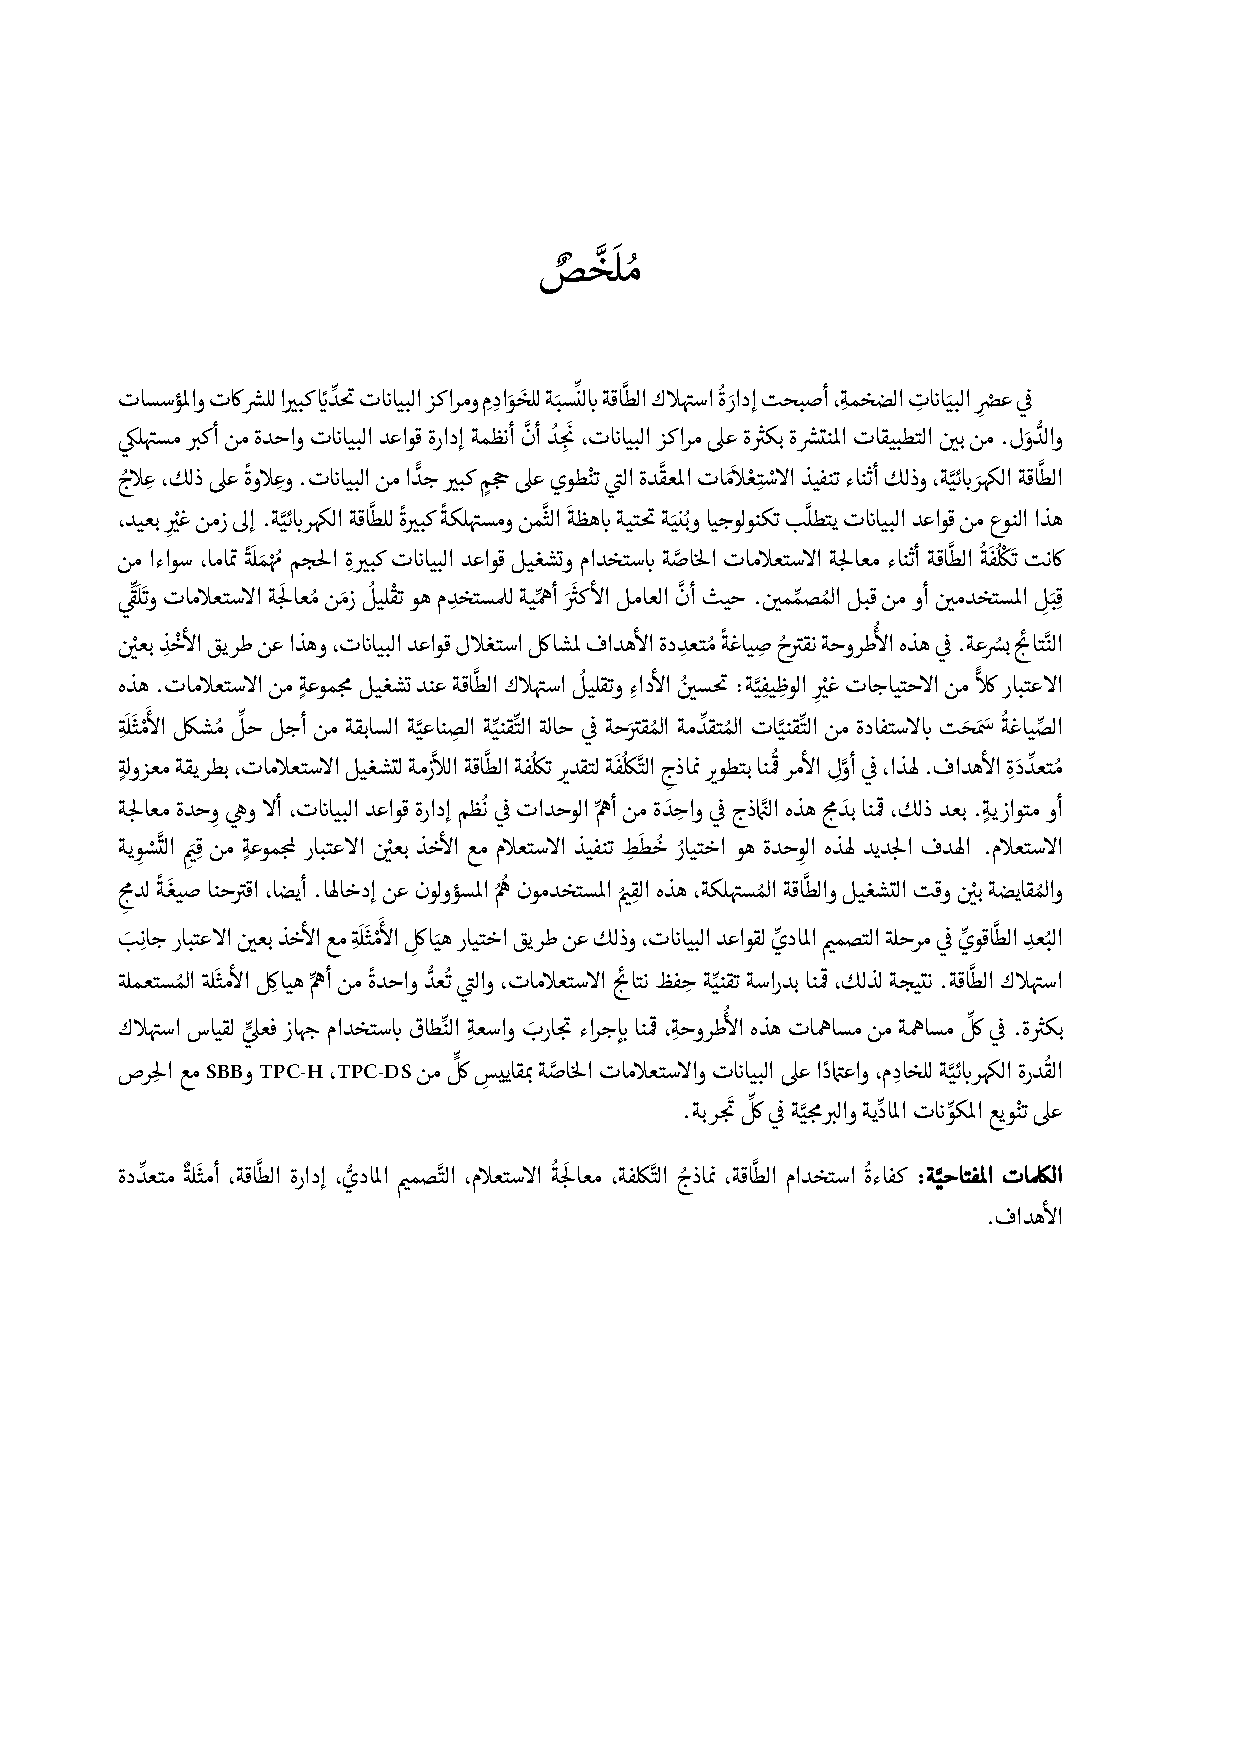
\includepdf[pages=-1]{include/abstract-arabic}
%--------------------------------------------------------
\begin{EnglishAbstract}
%\begin{spacing}{0.95}

In the Big Data Era, the management of energy consumption by servers and data centers has become a challenging issue for companies, institutions, and countries. In data-centric applications, Database Management Systems are one of the major energy consumers when executing complex queries involving very large databases.
Moreover, the processing of this type of data requires costly and energy-intensive computing and hardware infrastructures. Current practices in the use and exploitation of very large databases indicate that the energy cost of query is totally neglected by users and also by designers. Knowing that the most important factor for the user is minimizing the response time of queries. In this thesis we propose a multi-objective formalization of the databases exploitation techniques, taking into account two non-functional requirements: performance and energy consumption during the execution of a queries workload. This formalization allow us to take advantage of the advanced techniques proposed in the state-of-the-art for solving multi-objective optimization problems. For this purpose, we first develop cost models that estimate the energy consumption of queries executed in an isolated or parallel manner. These cost models are then integrated into one of the most important modules in a DBMS, which is the query processing module. The new objective of this module is the selection of execution plans of queries with the trade-off desired by the users between the time and the energy of the queries. Furthermore, we propose an initiative that integrates the energy dimension in the physical design phase of databases, in order to select optimization structures taking into account the energy aspects. We study the case of materialized views, one of the redundant optimization structures that is heavy used by database administrator. In each contribution of our thesis, intensive experiments are conducted using a real device for energy measurements and data of the TPC-H, TPC-DS and SBB benchmarks with various hardware and software configurations.

\KeyWords{Energy efficiency, cost models, query processing, physical design, energy management, multi-objective optimization.}

%\end{spacing}
\end{EnglishAbstract}
\end{ThesisAbstract}


%%-----------------------------------------------------------------
%% Remerciement
%%-----------------------------------------------------------------

\renewcommand{\AcknowledgmentName}{Remerciements}
\begin{ThesisAcknowledgments}

Je mesure la chance qui m'a été donnée d'être encadré par des personnes aussi impliquées, ouvertes et compétentes, qui ont cru en mes capacités pour mener à bien ce travail, et sans qui ce travail n'aurait jamais vu le jour. Qu'ils trouvent ici le témoignage de toute ma gratitude :

Ladjel BELLATRECHE, qui sait faire voler en éclat chaque idée reçue, qui s'est dévoué généreusement à ma thèse et qui m'a donné goût à la recherche. Il m'a fait énormément apprendre tant sur le plan scientifique qu'humain.

Omar BELHAMITI, pour son encadrement minutieux et ses bonnes qualités pédagogiques et scientifiques. Ses conseils avisés sont précieux et sa gentillesse m'est inégalé.

Un grand merci à Karim SEHABA, Djamal BENSLIMANE et Nadjia BENBLIDIA de m'avoir fait l'honneur d'être examinateurs de cette thèse, ainsi qu'à Amir ABDESSAMAD pour avoir accepté d'être membre du jury en tant que président. Je suis très honoré de l'intérêt qu'ils ont porté à mes travaux.

Mes remerciements vont également :

À Fouad HENNI qui a été toujours disponible pour m'apporter son aide. Ses conseils m'ont été très utiles, sa rigueur au travail est un exemple pour moi.
À Houari BENMEKKI qui m'a aidé à effectuer une partie de ma thèse à Poitiers et qui n'a jamais cessé de mettre à ma disposition les moyens qui m'ont permis d'aboutir cette thèse. À Emmanuel GROLLEAU, directeur du laboratoire LIAS/ENSMA pour son accueil et ses qualités humaines hors du commun.

À tous les membres d'Université de Mostaganem et du laboratoire LIAS, en particulier : Mohamed, Saliha, Asma, Djamila, Amel, Walid, Amin, Jalil, Maghnia, Liela, Houria et Sidahemd, ainsi que Ahcène, Selma, Sabrina, Abdelkader, Aymen, Lahcène avec lesquels j'ai
 partagé des moments inoubliables.

À mes amis et collègues sans exception, pour leur présence, leur respect et leur gentillesse.

Je ne saurais finir sans exprimer mes remerciements aux personnes qui me sont les plus proches :
Mon feu Père, à qui j'adresse un retentissant hommage, pour qui entre autres, j’ai spécialement porté cette tenue aujourd’hui, et à ma Mère, pour avoir pu cimenter ma vie dans un douillet cocon familial, fait d’amour, de bravoure et de zèle au travail; Mes deux frères Abdelatif et Sofiane, qui étaient toujours présents pour m'aider et me réconforter.

Et enfin, merci à tous ceux qui ont participé de près ou de loin à l’aboutissement de ce travail.

\end{ThesisAcknowledgments}

 % To-Uncomment

%-------------------------------------------------------------------
%                            dedicace
%-------------------------------------------------------------------
\begin{ThesisDedication}
En Hommage à mon Père, que ton âme repose en paix !\\ 
À tous ceux qui me sont chers :\\
Ma mère,\\
Mes frères.
\end{ThesisDedication}

%%-----------------------------------------------------------------
%% Table des matières avec chapitre encadré
%%-----------------------------------------------------------------

{
\hypersetup{linkcolor=black}
\dominitoc
\WritePartLabelInToc
\WriteChapterLabelInToc
%\FramePartsInToc
\tableofcontents

%%-----------------------------------------------------------------
%% % Inclusion de la liste des figures et des tables
%%-----------------------------------------------------------------

\WriteThisInToc
%\listoffigures
%\listoftables
{\listoffigures \let\cleardoublepage\clearpage \listoftables}
} % end hypersetup 

%%-----------------------------------------------------------------
%% Vocabulaire et notations utilisés
%%-----------------------------------------------------------------

% la numérotation commence à partir d'ici
\mainmatter

%%-----------------------------------------------------------------
%% Inclusion de chaque chapitre de la thèse
%%-----------------------------------------------------------------

\part{Introduction Générale}
\chapter{Introduction Générale}
\label{chap1} 

\epigraph{<< Et au-dessus de tout homme détenant la science, il y a un savant plus docte que lui. >>}{--- \textup{Joseph, v. 76}}
%\epigraph{<< Acquire knowledge, and learn tranquility and dignity. >>}{--- \textup{Omar ibn al-Khattab}}

\NoChapterPrefix \NoChapterNumberInRef {\hypersetup{linkcolor=black} \minitoc}

%% numérotation des figures, des tables et des équations préfixé par le numéro de chapitre
\makeatletter
\renewcommand{\thefigure}{\ifnum \c@section>\z@ \thechapter.\fi
 \@arabic\c@figure}
\@addtoreset{figure}{chapter}
\makeatother

\makeatletter
\renewcommand{\thetable}{\ifnum \c@section>\z@ \thechapter.\fi
 \@arabic\c@table}
\@addtoreset{table}{chapter}
\makeatother

\makeatletter
\renewcommand{\theequation}{\ifnum \c@section>\z@ \thechapter.\fi
 \@arabic\c@equation}
\@addtoreset{equation}{chapter}
\makeatother

\newpage
\section{Contexte et problématique}
Depuis quelques années, la communauté internationale regroupant les états, les gouvernements, les associations, et les usagers s'intéresse de près  aux changements climatiques en proposant des initiatives pour limiter le réchauffement climatique. En 2015, la France a organisé à Paris la Conférence mondiale des parties à la Convention-cadre de l'ONU portant sur cette problématique, appelée aussi << COP 21 >>, où 195 pays étaient représentés. L'un des objectifs primordiaux  de cette convention est de sensibiliser les \textit{pays pollueurs} et proposer des initiatives accompagnées par des solutions durables pour réduire le réchauffement climatique lié aux gaz à effet de serre (émissions de carbone ou $CO_2$). Rester immobiles de la part de la communauté internationale et les usagers  entrainera les conséquences néfastes sur la planète comme :  \textbf{(a)} la multiplication des vagues de chaleur, \textbf{(b)} des sécheresses et des inondations, \textbf{(c)} la fonte accélérée des glaciers. 

Depuis quelques années, un nombre important d'initiatives ont été menées couvrant plusieurs secteurs comme le \textit{bâtiment} (\textit{green house}) \cite{Perez08}, \textit{l'automobile} (l'émergence des voitures électriques) \cite{Tie13}, \textit{l'électronique} \cite{Barbose13}, \textit{les réseaux sans fil} \cite{Rault14}, etc. Les expériences énergétiques menées dans ces secteurs doivent être \textit{généralisées} et \textit{capitalisées} afin de les \textit{reproduire} et les \textit{réutiliser} dans d'autres secteurs dans lesquels l'énergie électrique n'est pas complètement intégrée. Pour illustrer ces avancées, nous prenons l'exemple du secteur du bâtiment qui a connu d'énormes progrès sur la prise en compte de l'énergie. Il est intéressant de noter qu'il est parmi les plus grand consommateurs d'énergie. En France par exemple, il représente 43\% des consommations énergétiques, soit 1,1 tonne équivalent pétrole par an et par habitant\footnote{\url{http://www.logement.gouv.fr/la-politique-energetique-dans-les-batiments-2445}}. D'après les dernières statistiques, le  poste << logement >> représente à lui seul 30\% du budget des ménages. Devant cette situation, plusieurs initiatives ont été prises pour réduire cette consommation que nous proposons de classer en deux catégories principales selon la nature du bâtiment : \textbf{(i)} les initiatives pour les bâtiments \underline{existants} et \textbf{(ii)} les initiatives pour les bâtiments \underline{neufs}. Pour les bâtiments existants, les pouvoirs publics ont beaucoup communiqué afin de sensibiliser et inciter les usagers à réduire leur consommation énergétique afin qu'ils aient un comportement \underline{éco-citoyens}. Des gestes simples pourraient contribuer à cette réduction. Nous pouvons citer par exemple : \textbf{(a)} s'arranger pour que les appareils électriques fonctionnent à pleine charge, \textbf{(b)} penser aux heures creuses pour la mise en route des appareils, \textbf{(c)} acheter des  appareils ménagers en tenant compte leur niveau de consommation électrique, \textbf{(d)} limiter le plus possible le nombre d'appareils en veille, \textbf{(e)} utiliser des ampoules basse énergie. Pour une réduction maximale d'énergie, ces gestes doivent concerner tout composant électrique du bâtiment susceptible de contribuer à la réduction de la consommation énergétique.  

En ce qui concerne les initiatives pour les bâtiments neufs, l'intégration de l'énergie est prise en compte dès la conception de ce dernier. Plusieurs réglementations ont été mises en place concernant l'utilisation des matériaux et équipements plus performants et à l'utilisation des énergies. Afin d'assurer un maximum de réduction énergétique, les deux types d'initiatives doivent être combinées. Sur le plan humain, tous les acteurs de la chaîne de construction de bâtiments : les \textit{concepteurs}, les \textit{producteurs} de matériaux de construction et les \textit{usagers} doivent travailler ensemble pour assurer cet objectif. 

Revenons à notre domaine d'étude qui est l'informatique. Ce secteur avec ses composantes (matérielles et logicielles) et ses usagers participe intensivement au phénomène de réchauffement climatique. L'une des causes principales de cette situation est la demande continuelle de calcul intensif du \textit{déluge de données} générées par les contenus numériques, les applications autour des \textit{données massives} (<< Big Data >>), l'\textit{E-commerce}, et le \textit{trafic Internet}. En conséquence, les centres de données deviennent l'épine dorsale pour toute entreprise, organisme et fournisseur de stockage de données comme \textit{Amazon}, \textit{Facebook}, \textit{Google}, etc. Si nous nous référons au Conseil de Défense des Ressources Naturelles, il a indiqué que les centres de données ont consommé 91 milliards de kilowatt-heures en 2013 \cite{NRDC14b}. Ceci représente environ 3\% de la consommation d'électricité mondiale, avec un coût annuel de 9 milliards de dollars \cite{Koomey11}. Citons l'exemple du centre de données construit par \textit{Interxion}, l'installation consomme 64 mega-watts, soit l'équivalent d'une ville de 50 000 habitants\footnote{\url{http://www.interxion.com/fr/Implantations/france/paris/par7/}}. Avec la chaleur qu'ils dégagent, ils génèrent 200 millions de tonnes de gaz à effet de serre \cite{NRDC14b}; Malheureusement, pour les défenseurs de l'environnement, cette situation ne fait que s'empirer. Les experts du secteur, tels que le SMARTer 2020, rapportent que la consommation des centres de données mondiaux augmenteront de 7\% chaque année jusqu'en 2020 \cite{SMARTer12}, en raison du développement d'Internet et de l'augmentation des besoins de stockage des entreprises.

La consommation énergétique électrique de ces centres est répartie de la manière suivante : \textbf{(i)} le matériel informatique déployé sur ces centres tels que serveurs de traitement, \textbf{(ii)} le stockage et la communication, \textbf{(iii)} des équipements de refroidissement d'infrastructure (pour un kilowatt dépensé par un serveur, un autre kilowatt serait nécessaire pour le refroidir \cite{Emerson07, Tsirogiannis10}) et \textbf{(iv)} leur fonctionnement sans arrêt. \ref{fig:datacenters-energy} illustre la distribution de consommation d'énergie des équipements informatiques dans un centre de données. Nous remarquons que le processeur, la mémoire et le disque consomment la moitié d'énergie totale.

\begin{figure}
    \begin{center}
        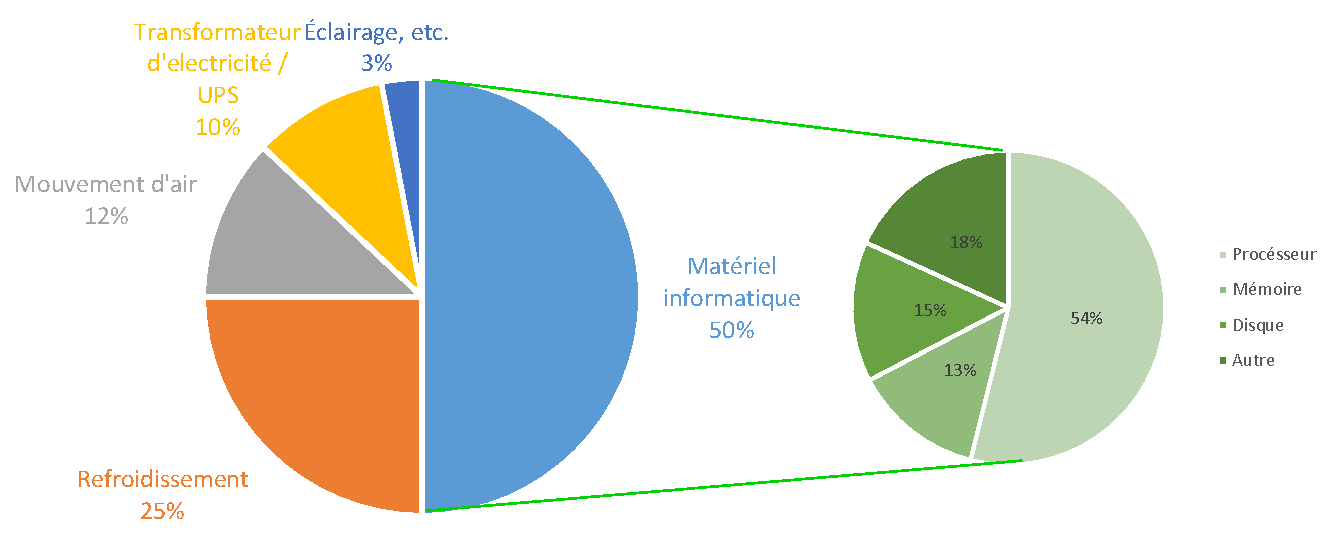
\includegraphics[scale=0.7]{chapitre1/chap1Fig/datacenters-energy.eps}
        \caption{La consommation d'énergie dans un centre de données.}
        \label{fig:datacenters-energy}
    \end{center}
\end{figure}

Face à cette situation, les industriels et les chercheurs de la communauté scientifique ne sont pas restés indifférents, ils ont pris des initiatives accompagnées de solutions réelles couvrant plusieurs actions, à savoir : \textbf{(a)} la conception de matériel avec une consommation énergétique réduite, \textbf{(b)} la restructuration des logiciels pour minimiser la consommation, \textbf{(c)} l'exploitation de divers états d'alimentation disponibles dans les nouveaux matériaux, et \textbf{(d)} une bonne conception, utilisation et contrôle de l'infrastructure des centres de données \cite{Kant09}. Ces actions ressemblent fortement à celles utilisées dans le secteur du bâtiment. Plus précisément: 
\begin{itemize}
	\item En ce qui concerne la conception de matériel avec une consommation énergétique réduite, les producteurs ont mis en place un label, appelé \textit{l'efficacité énergétique} (communément appelée PUE - power usage effectiveness) mesurant la quantité d'énergie totale consommée par un centre de données. Le consortium International Green Grid\footnote{\url{http://www.thegreengrid.org/}}, crée en 2007 et qui regroupe 501 membres et plus de 200 sociétés mondiales, vise au << verdissement >> des centres de données. L'ETSI (European Telecommunications Standards Institute) -- institut de normalisation européen des télécoms -- propose en juin 2014, une nouvelle mesure de l'efficacité énergétique comparable à celle que l'on retrouve déjà dans l'électroménager\footnote{\url{http://www.etsi.org/news-events/news/798-2014-06-press-etsi-releases-the-first-global-kpi-on-energy-efficiency-in-ict}}. Celle-ci comporte 5 niveaux de performance, du A << vert >> au I << noir >>, en passant par le G << rouge >>;
	\item En général, l'efficacité énergétique n'est pas synonyme d'efficacité de calcul \cite{Kant09}. En particulier, des techniques comme le regroupement des calculs et des transferts de données améliorent l'efficacité énergétique des logiciels. Cela est du fait qu'elles allongent les périodes d'inactivité et permettent aux dispositifs d'entrées/sorties dans des états de faible puissance. En outre, certaines opérations consomment moins d'énergie que d'autres pour un travail effectif équivalent. Il est intéressant de noter qu'une progression remarquable est constatée dans le développement de logiciels embarqués économiques. Cependant, il manque encore un travail considérable en terme  méthodologique, conceptuel, et validation pour le développement de logiciels économiques de tout bord \cite{Kant09}.
	\item De nos jours, presque tous les principaux composants d'un serveur offrent des modes de contrôle d'énergie. Ils se matérialisent sous forme d'états de puissance : une collection de modes opérationnels qui compromettent la consommation d'énergie pour la performance. Un état de puissance pour un composant est dit \textit{actif} si celui-ci reste opérationnel dans cet état, sinon l'état est dit \textit{inactif}. L'ACPI (\textit{Advanced Configuration and Power Interface}) fournit une nomenclature standard pour ces états et définit également les interfaces logicielles pour les gérer. L'ACPI est implémentée dans tous les principaux systèmes d'exploitation (\acrshort[hyper=false]{SE}) sous forme de la gestion de l'alimentation dirigée par le SE\footnote{\url{http://www.uefi.org/sites/default/files/resources/ACPI_6_1.pdf}}.
	\item Plusieurs technologies sont actuellement envisagées pour rendre l'infrastructure d'un centre de données plus efficace. Par exemple, la plupart des serveurs fonctionnent à une utilisation relativement faible la plupart du temps. Cependant, une double alimentation redondante (PSU) est souvent utilisée pour la fiabilité, ce qui se traduit par une charge et une efficacité relativement faible. Pour les infrastructures de refroidissement; dans une démonstration de concept d'un centre de données exploité par Intel, le refroidissement ambiant avec un échange d'air jusqu'à 32° a été utilisé. Le résultat obtenu est une économie de 67\% de puissance avec un refroidissement ambiant 91\% du temps \cite{Atwood08}. En descendant la hiérarchie, des solutions de refroidissement plus intelligentes ont émergé au niveau du châssis, des enceintes et du serveur sous la forme de ventilateurs à vitesse variable modulés par des mesures de température \cite{Kant09}.
\end{itemize}

La discussion ci-dessous que nous avons initiée concerne le domaine informatique d'une manière générale. Nous nous focalisons sur un de ses postes importants à savoir les systèmes de gestion de données (\acrshort[hyper=false]{SGBD}), ou les systèmes de stockage de donnée hébergés par les centres de données. Ceci représente le contexte de cette thèse. Les SGBD sont les plus gros consommateurs d'énergie électrique. Cela est dû au fait qu'ils effectuent des opérations (jointure, union, agrégation, etc. ), impliquant des tables ou des structures de données volumineuses qui nécessitent toutes les ressources d'un centre de données (CPU, mémoire, et  réseau). 

Devant cette situation critique, deux articles de vision ont été publiés par des chercheurs de la \textit{communauté de bases de données} provenant à la fois du milieu académique (Stavros Harizopoulos et al. \cite{Harizopoulos09} de MIT) et industriel (Goetz Graefe \cite{Graefe08} de HP). Ils ont mis l'accent sur l'intégration de l'énergie dans la conception et l'exploitation des bases de données. Les recommandations de ces auteurs coïncident avec ce que la communauté scientifique a identifié, à savoir l'utilisation des matériels et logiciels économiques \cite{PoessN08}. Les SGBD peuvent bénéficier des matériels économiques existants (comme les supports de stockage amovible \cite{Schall10}, les cartes graphiques \cite{Hurson16}, etc.).  

\begin{figure}
	\begin{center}
		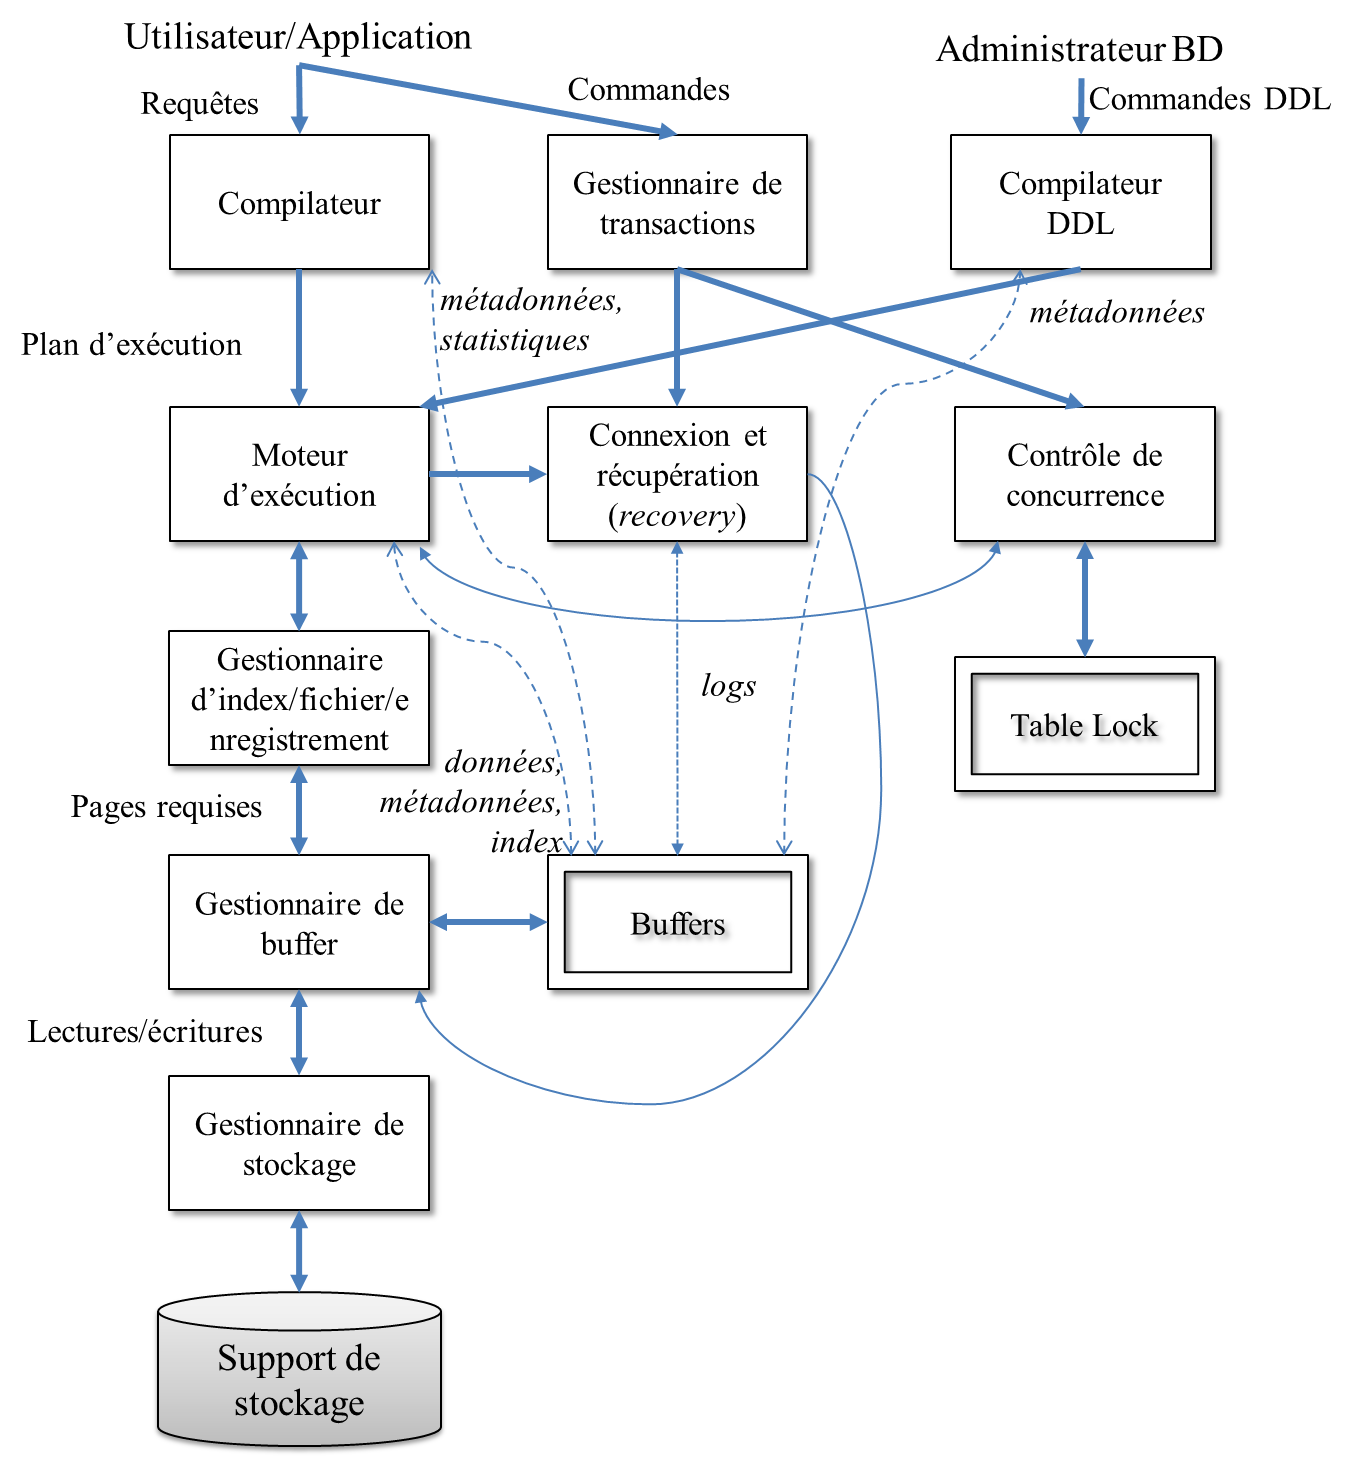
\includegraphics[scale=0.5]{chapitre1/chap1Fig/composantesSGBD.png}
		\caption{Les composantes principales d'un SGBD}
		\label{fig:composantesSGBD}
	\end{center}
\end{figure}

Rappelons que la consommation énergétique d'un SGBD dépend de la base de données qu'il héberge. Plus précisément, elle dépend de son schéma (le nombre de tables et les attributs), sa population (en termes d'instances) et son exploitation via des requêtes. La plus grosse consommation d'un SGBD est due au calcul effectué par ses composantes principales : l'optimiseur de requêtes, le gestionnaire de buffer, le contrôleur de concurrence, le gestionnaire des méthodes d'accès, le gestionnaire de stockage, etc. comme le montre la \ref{fig:composantesSGBD}. Les travaux existants sur l'incorporation de la dimension << énergie >> se focalise sur la partie traitement de requêtes. Ils supposent que la base de données est déjà conçue et déployée sur un SGBD. L'optimisation de requêtes dans les bases de données est une tâche difficile, et souvent modélisée comme un problème d'optimisation à base de contraintes. Ces dernières représentent plusieurs besoins non-fonctionnels comme le temps de réponse, le coût de stockage, le coût de maintenance. Les approches proposées pour résoudre cette problématique font souvent appel au développement de modèles de coût mathématiques estimant le ou les besoins non-fonctionnels utilisés. Les premiers travaux sur l'incorporation de l'énergie dans le monde des bases de données (côté logiciel) étaient le développement de modèles de coût mathématiques estimant la consommation énergétique lors de l'exécution de requêtes. Ces modèles prennent en compte des paramètres couvrant plusieurs entités logicielles et matérielles de la base de données cible tels que son schéma (par ex. la taille des tables, la longueur de tuples, etc.), la charge de requêtes (par ex. le type de requêtes, les facteurs de sélectivité des jointures et des prédicats de sélections, tailles des résultats intermédiaires, etc.), le matériel (par ex. la taille de tampon, la taille de page du disque, etc.) et la plate-forme de déploiement (par ex. RAM, la taille du disque, le nombre de nœuds, etc.).

D'autres efforts ont été effectués dans le développement des bancs d'essai permettant aux chercheurs de tester l'efficacité de leurs modèles économiques dédiés à la gestion de la base. Nous pouvons citer l'exemple du banc d'essai TPC-Energy \cite{TPCE} lancé en 2007. 

L'ensemble de ces travaux suppose que la base de données est déjà déployée et s'intéresse particulièrement à la partie optimisation de requêtes effectuée par le SGBD hébergeant cette base. Or, d'autres phases de cycle de vie de la base de données peuvent être sensibles à l'énergie comme la phase physique -- souvent associée à l'image de la qualité et de performance de toute base de données -- dans la quelle des structures d'optimisation comme les index, les vues matérialisées, le partitionnement doivent être sélectionnées. Ces structures sont souvent utilisées par les optimiseurs de requêtes pour finir des plans efficaces (\ref{fig:cyclehors}).

\begin{figure}
	\begin{center}
		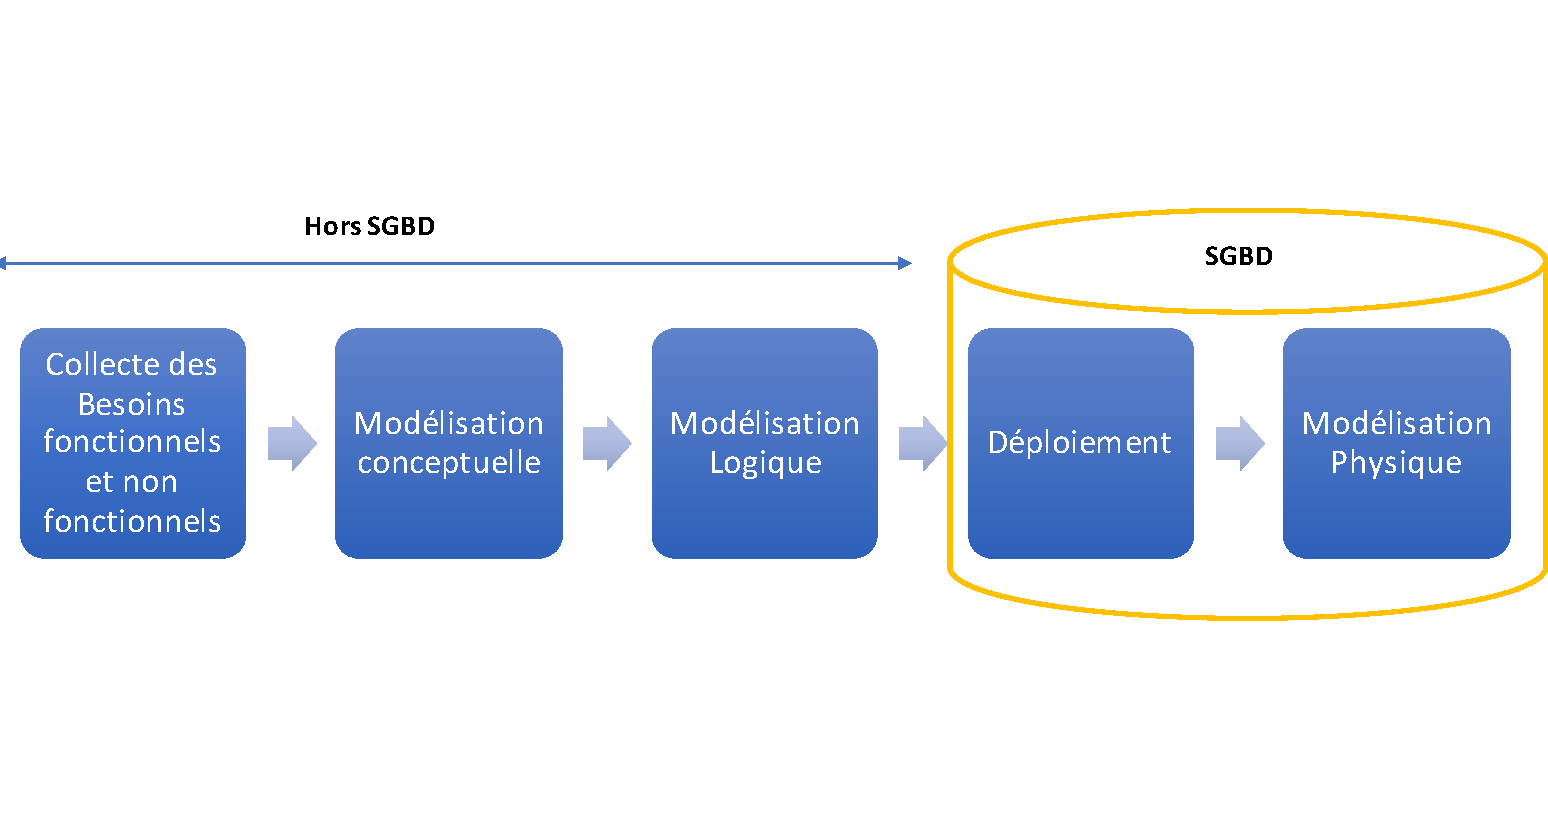
\includegraphics[scale=0.5]{chapitre1/chap1Fig/cyclehors.pdf}
		\caption{L'énergie dans le cycle de vie de conception de base de données}
		\label{fig:cyclehors}
	\end{center}
\end{figure}

Dans cette thèse, nous tenterons à répondre à ces limites en proposant des modèles mathématiques plus robustes pour estimer l'énergie et proposer une démarche de conception physique dirigée par la consommation énergétique. 

Dans les sections suivantes, nous présentons les objectifs de notre thèse et l'ensemble de contributions réalisées.

\section{Objectifs et contributions}
Notre premier objectif est de sensibiliser les usagers et les concepteurs de bases de données de la dimension énergétique, en suivant l'expérience du domaine du bâtiment, en proposant des solutions pour des bases de données déjà existantes. Cela doit passer par la revisite des travaux sur l'optimisation de requêtes, considérée comme un poste gourmand en énergie. L'intégration de l'énergie dans les optimiseurs de requêtes peut se faire en suivant plusieurs scénario : (i) les optimiseurs de requêtes dirigées par seulement l'énergie, (ii) les optimiseurs de requêtes dirigées par plusieurs besoins non-fonctionnels y compris l'énergie. Dans la continuité de la reproduction des efforts du secteur du bâtiment, nous avons déployé nos solutions énergétiques sur un SGBD open source (PostgreSQL) afin de valider nos résultats et surtout pour sensibiliser et motiver les usagers et les concepteurs pour intégrer cette dimension dans leurs solutions. 
Le second objectif est de pousser plus loin notre réflexion sur la conception verte des bases de données, et l'appliquer sur une autre phase de cycle de vie qui est la phase physique. 

Afin de répondre à nos objectifs, nous nous sommes fixées un ensemble d'actions qui sont : 
\begin{enumerate}
	\item \textit{Un audit sur les composants d'un SGBD.} Pour économiser l'énergie, il faut d'abord identifier les postes sensibles. Cela est établi par un audit de l'ensemble de composants d'un SGBD (\ref{fig:composantesSGBD}). Dans un serveur informatique, il y a généralement cinq consommateurs d'énergie, à savoir, le processeur, les disques, la mémoire, les dispositifs d'entrées/sorties (\acrshort[hyper=false]{E/S}) et la carte mère. Il faut étudier le comportement du système lors de l'exécution d'une requête par le SGBD et son impact sur l'énergie. Atteindre une efficacité énergétique nécessite des améliorations dans le profil de la consommation d'énergie de chaque composant du système.
	\item \textit{L'adoption dynamique de composants matériels.} L'adoption de composants matériels dynamiquement pourrait aider à améliorer l'efficacité énergétique. Par exemple, l'exécution du processeur à une fréquence inférieure permet de réduire la tension, résultant d'une économie d'énergie. Cette technique, qui met en œuvre un compromis entre la performance et l'énergie, est connue comme l'ajustement dynamique de la tension et de la fréquence (\acrshort[hyper=false]{DVFS}), la tension et la fréquence sont ajustées à la volée. Une technique similaire existe pour les disques et mémoires vivres \cite{Sjalander14}.
	En outre, en employant des lecteurs de disques \gls{SSD}, des cartes graphiques puissantes pour le traitement, une grande configuration de mémoire, processeurs et mémoires de faible consommation ont pourrait diminuer la consommation d'énergie totale du système.
	Intégrer ces techniques directement dans l'SGBD afin de contrôler son bon fonctionnement est nécessaire, car le SGBD a la connaissance sur la donnée. 
	\item \textit{Le développement des modèles de coût mathématiques}. Toute prise de décision d'un SGBD est souvent orchestrée par un modèle  de coût mathématique estimant un besoin non-fonctionnel. Dans le contexte de l'energie, l'optimiseur de requêtes doit être associé à des modèles de coût robustes qui doivent prendre en compte tous des paramètres pertinents des composantes sensibles à l'énergie électrique. 
	\item \textit{Vers une sélection des structures d'optimisation vertes}. Les structures d'optimisation  (les vues matérialisées, les index, etc.) qui ont émergé avec l'arrivée des entrepôts de données sont souvent sélectionnées avec des algorithmes dirigés par des modèles de coût mathématiques, estimant la performance de requêtes ou le coût de maintenance. Cette sélection doit être revisitée pour intégrer le coût énergétique. 
\end{enumerate}
Dans cette thèse nous considérons les actions (1), (3) et (4). L'action (2) n'est pas considéré dans notre étude pour plusieurs raisons :
\begin{itemize}
	\item Les techniques basées sur le matériel requièrent de nouveaux matériels, car d'une part les nouvelles technologies comme le DVFS ne sont pas disponibles sur tout les processeurs et d'autre part les nouveaux disques SSD sont très cher et ont un problème de durée de vie. 
	\item Il existe diverses gammes pour chaque composant matériel, donc développer des méthodes sur une seule gamme ou marque limite la portabilité de ces méthodes.
	\item Les techniques logicielles sont préférées dans le contexte des bases de données car le SGBD a une connaissance détaillée sur les charges de requêtes, les plans d'exécution, les informations sur les données, etc.
\end{itemize}

Pour répondre aux limitations précédentes, nos principales contributions, décrites dans cette thèse, sont les suivantes :
\begin{description}
	\item[La proposition d'un modèle de coût énergétique pour des requêtes isolées.] Pour exécuter une requête \acrshort[hyper=false]{SQL}, l'optimiseur doit sélectionner son meilleur plan d'exécution qui peut être représenté par un arbre d'opérations algébriques correspondant à cette requête. Une fois identifié, l'optimiseur exécute ce plan étape par étape\footnote{Ce mode d'exécution est appelé le mode itérateur.}. Le mode d'exécution des requêtes influence la puissance électrique consommée et l'énergie totale. Cette observation est complètement ignorée par les travaux de l'état de l'art lors de la définition des modèles de coût. Ce dernier doit prendre en considération la relation entre les paramètres du modèle (linéaire, logarithmique, exponentielle. etc.) pour avoir des résultats fiables. Les travaux existants supposent que cette relation est linéaire. Dans cette thèse, nous avons montré que la relation est non-linéaire. 
	
	\item[Modèle de coût énergétique pour des requêtes concurrentes.] Dans un environnement réel des centres de données, le SGBD exécute un ensemble de requêtes simultanément de façon concurrente. Cette hypothèse n'est pas prise en compte par les travaux existants lors de la définition des modèles de coût. En conséquence, nous avons  étendu notre modèle de coût pour prendre en charge ce scénario. Cela est utile pour plusieurs tâches telles que le contrôle d'admission, l'ordonnancement des requêtes et le contrôle d'exécution des requêtes avec l'objectif d'améliorer l'efficacité énergétique.  
	
	\item[Traitement de requêtes éco-énergétique.] Avec la présence de modèle de coût, nous proposons une  méthodologie qui intègre l'énergie dans le processus de traitement des requêtes pour produire des plans d'exécutions réduisant leur consommation. Cette démarche a été implémentée sous le SGBD PostgreSQL.
	
	\item[Conception physique éco-énergétique.] Nous avons proposé une approche de sélection de structures d'optimisation en prenant en compte plusieurs besoins non-fonctionnels : la performance de requêtes, l'espace de stockage et la consommation énergétique. Nous avons choisi le cas des vues matérialisées; considérées comme des structures redondantes du fait qu'elles exigent une espace de stockage et un coût de maintenance. Nous avons alors formalisé le problème de sélection des vues matérialisées comme un problème multi-objectif et nous avons proposé des algorithmes avancés pour sa résolution.                     
	 \end{description}

\section{Organisation de la thèse}

% TODO: update graph, use Fig1.3 of Beloglazov11 thesis
\begin{figure}
	\begin{center}
		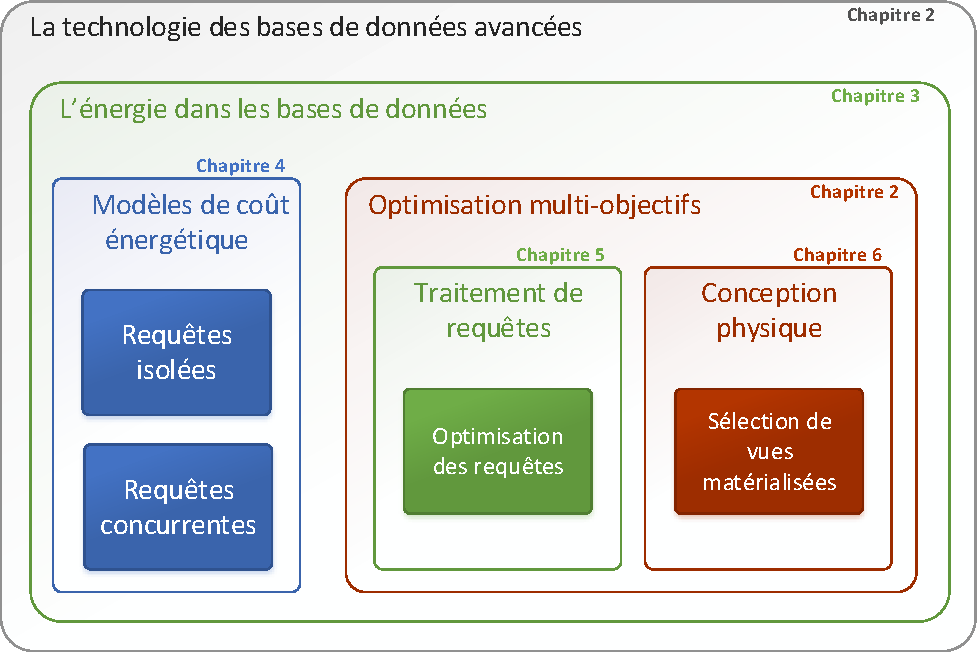
\includegraphics[scale=0.7]{chapitre1/chap1Fig/chapters-org2.pdf}
		\caption{La répartition des chapitres de la thèse.}\label{fig:chapitres}
	\end{center}
\end{figure} 

D'un point de vue organisationnel, le reste de la thèse s'articule autour de six chapitres.

Dans le \ref{chap2}, nous présentons un état de l'art sur le cycle de vie de conception des bases de données avancées, avec une focalisation particulière sur la phase physique. Le chapitre décrit aussi le module de traitement de requêtes dans un SGBD relationnel et propose la conception d'un optimiseur de requêtes éco-énergétique. Le chapitre cite également les techniques d'optimisations multi-objectifs et les solutions proposées dans le contexte des bases de données pour sa résolution.

Dans le \ref{chap3}, nous présentons un état de l'art sur les différentes techniques d'amélioration de l'efficacité énergétique dans les systèmes informatiques en général, et dans les bases de données en particulier, les différents concepts requis pour ce travail ainsi que les notions de bases sur l'énergie et les modèles de coût proposés sont présentés.

Dans le \ref{chap4}, nous étudions le comportement de l'énergie des bases de données sur le matériel informatique. Il s'agit d'identifier les paramètres et ses caractéristiques liées à la consommation énergétique des requêtes. A la base de cette étude empirique, nous proposons un modèle de coût pour estimer la consommation énergétique d'une requête SQL isolée. Ensuite, le cas des requêtes exécutées simultanément de façon concurrente est étudié. Nous étendons le modèle coût pour une seule requête vers une charge de requêtes, et nous adaptons les paramètres et les algorithmes pour avoir une meilleure estimation. Nous validons notre modèle sur une variété de configurations logicielles et matérielles. 

Dans le \ref{chap5}, nous étudions le cas de traitement des requêtes dans un SGBD relationnel, afin de savoir l'impact de chaque phase de ce traitement sur la consommation d'énergie du système. Suivant cette étude, nous proposons une méthodologie qui intègre l'énergie dans le processus de traitement des requêtes pour produire des plans d'exécutions réduisant la dissipation d'énergie.

Le \ref{chap6} aborde le problème d'intégration de l'énergie dans la phase de conception physique des bases de données. L'analyse est effectuée en prenant le cas des vues matérialisées. Une formalisation multi-objectif est proposée, et un algorithme évolutionnaire est utilisé pour résoudre le problème de sélection des vues matérialisées.

En fin, nous concluons la thèse par un bilan général sur nos contributions, et l'évocation des perspectives qui s'offrent à l'issue de notre travail dans le \ref{chap7}.

Ce mémoire comprend également trois annexes. L'\ref{annex:CostModelEstimations} décrit le processus d'estimation des coûts dans la phase d'optimisation des requêtes dans un SGBD. Elle donne les fonctions d'estimation de cardinalité des résultats intermédiaires, et détaille les formules d'estimation du coût d'entrées/sorties des opérateurs physiques. L'\ref{annex:ConfidenceBounds} étudie les bornes de confiance dans les données et les résultats de modèle de coût énergétique afin de confirmer la qualité de la modélisation. L'\ref{annex:TrainQueries} liste les requêtes utilisées pour construire le modèle de coût énergétique lors de la phase d'apprentissage.

Les principales contributions de notre thèse sont réparties dans les Chapitres \ref{chap4}, \ref{chap5} et \ref{chap6}. La \ref{fig:chapitres} schématise les grands axes de ce travail et leur répartition dans chaque chapitre.
Chacun des ces chapitres a donné lieu à un ensemble de communications et de publications dans des conférences internationales :

\textbf{Publications internationales :}

\begin{quote}
	\cite{Roukh17} 
	\textbf{Amine ROUKH}, Ladjel BELLATRECHE, Selma BOUARAR, Ahcène BOUKORCA : Eco-Physic: Eco-Physical Design Initiative for Very Large Databases. Information Systems. Elsevier, 2017. \href{http://dx.doi.org/10.1016/j.is.2017.01.003}{\textsc{[doi]}}.
\end{quote}

\textbf{Communications internationales :}

\begin{quote}
	\cite{Roukh15a} \textbf{Amine ROUKH}, Ladjel BELLATRECHE : Eco-Processing of OLAP Complex Queries. In proceedings of 17th International Conference on Big Data Analytics and Knowledge Discovery (DAWAK). LNCS, Springer, Valencia, Spain, September 1-4, 2015. p. 229-242. \href{http://dx.doi.org/10.1007/978-3-319-22729-0_18}{\textsc{[doi]}}.                                                                                                                                                                                                                                                                               \end{quote} 

\begin{quote}
	\cite{Roukh15b} \textbf{Amine ROUKH} : Estimating Power Consumption of Batch Query Workloads. In proceedings of 5th International Conference Model and Data Engineering. Springer International Publishing (MEDI), Rhodes, Greece, September 26-28, 2015. p. 198-212. \href{http://dx.doi.org/10.1007/978-3-319-23781-7_16}{\textsc{[doi]}}.
\end{quote}

\begin{quote}
	\cite{Roukh15c} 
	\textbf{Amine ROUKH}, Ladjel BELLATRECHE, Ahcène BOUKORCA, Selma BOUARAR : Eco-DMW: Eco-Design Methodology for Data Warehouses.  In proceedings of 15th International Workshop on Data Warehousing and OLAP (DOLAP). ACM, Melbourne, Australia, October 23 - 23, 2015. p. 1-10. \href{http://dx.doi.org/10.1145/2811222.2811230}{\textsc{[doi]}}. 
\end{quote}

\begin{quote}
	\cite{Roukh16a} \textbf{Amine ROUKH}, Ladjel BELLATRECHE, Carlos ORDONEZ : EnerQuery: Energy-Aware Query Processing.  In proceedings of 16th International on Conference on Information and Knowledge Management (CIKM). ACM, Indianapolis, Indiana, USA — October 24 - 28, 2016. p. 2465-2468. \href{http://doi.acm.org/10.1145/2983323.2983334}{\textsc{[doi]}}.
\end{quote}

\begin{quote}
	\cite{Roukh16b} \textbf{Amine ROUKH}, Ladjel BELLATRECHE, Nikos TZIRITAS, Carlos ORDONEZ : Energy-Aware Query Processing on Parallel Database Cluster Nodes. In proceedings of 16th International Conference on Algorithms and Architectures for Parallel Processing (ICA3PP). Springer International Publishing, Granada, Spain, December 14-16, 2016. p. 260-269. \href{http://dx.doi.org/10.1007/978-3-319-49583-5_20}{\textsc{[doi]}}.
\end{quote}

\begin{quote}
	\cite{Ouared16} Abdelkader OUARED, Yassine OUHAMMOU, \textbf{Amine ROUKH} : A Meta-advisor Repository for Database Physical Design. In proceedings of 6th International Conference on Model and Data Engineering (MEDI) Springer International Publishing, Almería, Spain, September 21-23, 2016. p. 72-87. \href{http://dx.doi.org/10.1007/978-3-319-45547-1_6}{\textsc{[doi]}}.
\end{quote}

\begin{quote}
	\cite{Bouarar17} Selma BOUARAR, Ladjel BELLATRECHE, \textbf{Amine ROUKH} : Eco-Data Warehouse Design Through Logical Variability. In proceedings of 43rd International Conference on Current Trends in Theory and Practice of Informatics (SOFSEM). Springer International Publishing, Limerick, Ireland, January 16-20, 2017. p. 436-449. \href{http://dx.doi.org/10.1007/978-3-319-51963-0_34}{\textsc{[doi]}}.
\end{quote}

% La répartition des publications et des communications à travers nos chapitres est la suivante :
% \begin{itemize}
% 	%\item Chapitre 3 : \cite{}.
% 	\item Chapitre 4 : \cite{Roukh15a, Roukh15b}.
% 	\item Chapitre 5 : \cite{Roukh16a, Roukh16b}.
% 	\item Chapitre 6 : \cite{Roukh15c}.
% 	%\item Chapitre 6 : \cite{}.
% \end{itemize}
\part{État de l'art}
\chapter{La technologie des bases de données}
\label{chap2}

\epigraph{<< The beginning of knowledge is the discovery of something we do not understand. >>}{--- \textup{Frank Herbert}}

\NoChapterPrefix \NoChapterNumberInRef {\hypersetup{linkcolor=black} \minitoc}

%% numérotation des figures, des tables et des équations préfixé par le numéro de chapitre
\makeatletter
\renewcommand{\thefigure}{\ifnum \c@section>\z@ \thechapter.\fi
 \@arabic\c@figure}
\@addtoreset{figure}{chapter}
\makeatother

\makeatletter
\renewcommand{\thetable}{\ifnum \c@section>\z@ \thechapter.\fi
 \@arabic\c@table}
\@addtoreset{table}{chapter}
\makeatother

\makeatletter
\renewcommand{\theequation}{\ifnum \c@section>\z@ \thechapter.\fi
 \@arabic\c@equation}
\@addtoreset{equation}{chapter}
\makeatother
%%-----------------------------------------------------------------
%% Résumé
%%-----------------------------------------------------------------

%laisser une page ou deux pages vides, telle est la question !
%\EmptyNewPage
\newpage

%********************************************************************************
%********************************************************************************
\section{Introduction}
Aujourd'hui, la disponibilité des systèmes de gestion de base de données fiables permet aux organisations de toutes tailles de gérer leurs données efficacement, de les stocker, et de déployer des applications exploitant ces données. Ces trois opérations fondamentales sont précieuses pour assurer la sécurité, l'intégrité des données et l’uniformisation des procédures administratives. Les bases de données sont actuellement au cœur des systèmes d’information des entreprises, plus particulièrement dans les tâches de gestion. Au cours des quarante dernières années, des concepts, des méthodes, et des algorithmes ont été développés pour gérer les données sur des mémoires secondaires, ils constituent aujourd’hui l’essentiel de la discipline << Bases de Données >> (\acrshort[hyper=false]{BD}). Cette discipline est utilisée dans de nombreuses applications. De plus, Il existe un grand nombre de Systèmes de Gestion de Bases de Données (SGBD), qui permettent de gérer efficacement des bases de données volumineuses. Dans ce contexte, une théorie fondamentale sur les techniques de modélisation des données, et les algorithmes de traitement a vu le jour. Les bases de données constituent donc une discipline s’appuyant sur une théorie solide et offrant de nombreuses solutions pratiques.

Dans ce chapitre, nous présentons un état de l'art portant sur la technologie des bases de données, son historique, son cycle de vie de conception et d'exploitation. Nous nous focalisons particulièrement sur la phase de conception physique et le traitement des requêtes. Nous allons détailler les différentes techniques utilisées et travaux proposés pour chacune d'entre elles. En second lieu, nous abordons les problèmes d'optimisation multi-objectifs en citant les méthodes de résolution proposées dans le cas général et le cas des bases de données.

\section{Technologie des bases de données}
Une base de données est un ensemble structuré de données enregistrées sur des supports accessibles par ordinateur, représentant des informations du monde réel et pouvant être interrogées et mises à jour par une communauté d’utilisateurs.

La gestion et l’accès à une base de données sont assurés par SGBD. Un Système de Gestion de Bases de Données est un logiciel de haut niveau permettant aux utilisateurs de structurer, d’insérer, de modifier, de rechercher de manière efficace des données spécifiques, au sein d’une grande quantité d’informations, stockées sur mémoires secondaires partagée de manière transparente par plusieurs utilisateurs.

% Evolution des DB et SGBD
% 2. HISTORIQUE DES SGBD (book: Bases de données, page: 42)
% resumé les parags

Suite à la progression de la technologie dans les domaines des processeurs, de la mémoire, du stockage et des réseaux informatiques, les tailles, les capacités et les performances des bases de données et SGBD ont augmenté en ordre de grandeur. Le développement de la technologie de base de données peut être divisé en trois périodes basées sur le modèle ou la structure de données: \textbf{navigationnelle}, \textbf{relationnelle} et \textbf{post-relationnelle} \cite{Chu07}.

% 1er génération
Lorsque les ordinateurs augmentaient en vitesse et en capacité, un certain nombre de systèmes de base de données à usage général ont vu le jour. Au milieu des années 1960, une partie de ces systèmes étaient utilisés commercialement. En 1971, le groupe de travail sur les bases de données au sein de la société CODASYL a livré son standard, qui est généralement connu sous le nom d'approche \textit{CODASYL} ou modèle réseau \cite{Bachman73}. Le produit commercial IDMS développé par Charles Bachman est basé sur cette approche \cite{Warren75}. L'approche CODASYL s'appuie sur des modèles de données organisés autour de types d’articles constituant les nœuds d’un graphe, reliés par des types de pointeurs composant les arcs du graphe.
IBM avait également son propre SGBD en 1966, connu sous le nom de système de gestion de l'information (IMS) \cite{IMS20360}. IMS était un développement de logiciels écrits pour le programme Apollo sur le système/360. IMS était généralement semblable en concept à CODASYL, mais a utilisé un modèle \textit{hiérarchie} stricte pour son modèle de navigation de données au lieu du modèle de réseau de CODASYL \cite{Bachman73}.

% 2eme génération
Le modèle \textit{relationnel}, proposé pour la première fois en 1970 par Edgar F. Codd \cite{Codd70}, s'est écarté de cette tradition en insistant sur le fait que les applications devraient chercher les données par contenu plutôt que par des liens. Le modèle relationnel utilise des ensembles de tables de style grand livre, utilisés chacun pour un type différent d'entité. Il s'agit d'un modèle mathématique défini en termes de logique de prédicat et de théorie des ensembles. IBM System R \cite{Chamberlin81} était un projet novateur, il s'agissait de la première implémentation de SQL, qui est devenu depuis le langage de requête de données relationnelles standard. Il a également été le premier système à démontrer qu'un système de gestion de base de données relationnelle pourrait fournir de bonnes performances de traitement des transactions. Ceci a poussé IBM à développer une véritable version de production de System R, connue sous le nom de SQL DS, et, plus tard, Database 2 (DB2).
Un autre modèle de données, le modèle \textit{entité-association} proposé par Peter Chen est apparu en 1976 \cite{Chen1976}. Ce dernier a gagné en popularité pour la conception des bases de données grâce à sa description des données plus familière que celle du modèle relationnel.

C'est seulement au milieu des années 1980 que le matériel informatique est devenu suffisamment puissant pour permettre un large déploiement de systèmes relationnels. Cependant, depuis le début des années 90, les systèmes relationnels demeurent dominant dans toutes les applications de traitement de données à grande échelle, tel que : IBM DB2, Oracle, MySQL, PostgreSQL et Microsoft SQL Server. Ils supportent en général une architecture répartie, avec des stations clients transmettant leurs requêtes à des serveurs puissants qui gèrent les bases de données. Le langage de base de données dominant le modèle relationnel est le SQL. Ce dernier a largement influencé les langages des autres modèles de données.

Les années 1990, parallèlement à une augmentation d'utilisation de la programmation \textit{orientée objet}, ont connu une croissance dans la façon dont les données dans diverses bases de données ont été traitées. Les programmeurs et les concepteurs ont commencé à traiter les données dans leurs bases de données comme des objets. C'est-à-dire que si les données d'une personne figuraient dans une base de données, les attributs de cette personne, comme son adresse, son numéro de téléphone et son âge, sont désormais considérés comme appartenant à cette personne au lieu d'être des données étrangères. Cela permet aux relations entre les données d'inclure des objets et leurs attributs et non des champs individuels \cite{Maier86}. Des systèmes commerciaux sont apparus, tel que Illustra, Objectivity/DB, Omniscience et UniSQL.

% 3eme génération
Les produits offrant un modèle de données plus général que le modèle relationnel sont classés comme post-relationnels, d'autres termes alternatifs incluent << base de données hybride >>, << base de données améliorée >>. Le modèle de données de ces produits incorpore des relations mais n'est pas limité par la contrainte de E.F. Codd, qui exige que : << \textit{toutes les informations dans la base de données doivent être exprimées explicitement en termes de valeurs dans les relations et d'aucune autre manière} >> \cite{Date99}. Un exemple est les bases de données \textit{XML}, qui sont un type de base de données structurée orientée document permettant d'interroger les attributs de document XML \cite{Chaudhri03}. Les bases de données XML sont principalement utilisées dans la gestion des bases de données d'entreprises, où XML est utilisé comme norme d'interopérabilité de données machine à machine. Les systèmes de gestion de base de données XML incluent les logiciels commerciaux MarkLogic et Oracle Berkeley DB XML, ainsi que les logiciels libres comme Clusterpoint Distributed XML/JSON et BaseX.

Certaines des extensions au modèle relationnel intègrent des concepts issus de technologies antérieures au modèle relationnel. Par exemple, ils permettent la représentation d'un graphe dirigé avec des arbres sur les nœuds, comme GraphDB et Neo4j. Certains produits post-relationnels étendent les systèmes relationnels en systèmes \textit{dimensionnels} utilisés pour représenter les données dans les entrepôts de données de façon à pouvoir facilement résumer les données en utilisant le traitement analytique en ligne ou les requêtes \acrshort[hyper=false]{OLAP}. Dans le modèle dimensionnel, un schéma de base de données se compose d'une seule grande table de faits qui est décrite en utilisant des tables de dimensions et des mesures. Des exemples de produits dans cette tendance est IBM InfoSphere Warehouse, Sybase IQ et Teradata Enterprise Data Warehouse.

Une autre tendance, dès les années 2000, dans la génération de post-relationnels est les bases de données \textit{NoSQL}. Les BDs NoSQL sont souvent très rapides et ne nécessitent pas de schémas de tables fixes. Ils évitent également les opérations de jointure en stockant des données dénormalisées et ils sont conçues pour être redimensionnées horizontalement \cite{Stonebraker10}. Déclenché par les besoins des entreprises comme Facebook, Google et Amazon devant le Web 2.0. La raison principale de l'émergence et de l'adoption des bases de données NoSQL est le développement des clusters de serveurs et la nécessité de posséder un paradigme de bases de données adapté à ce modèle d'infrastructure matérielle. Les bases de données NoSQL sont de plus en plus utilisées dans des applications << Big Data >> et web temps réel. Les structures de données utilisées par les bases de données NoSQL incluent le modèle clé-valeur, la colonne, le graphe et le document. Les systèmes NoSQL les plus populaires incluent MongoDB, Couchbase, Riak, Memcached, Redis, CouchDB, Hazelcast, Apache Cassandra et HBase\footnote{\url{http://db-engines.com/en/ranking}}, qui sont tous des logiciels libres.

\textit{NewSQL} est une classe de bases de données relationnelles modernes qui vise à fournir la même performance évolutive des systèmes NoSQL pour les charges de traitement transactionnel en ligne (lecture-écriture) tout en utilisant SQL et en maintenant les garanties les propriétés ACID (atomicité, cohérence, isolation et durabilité) d'un système de base de données traditionnel \cite{Stonebraker12}. Ces bases de données incluent ScaleBase, Clustrix, EnterpriseDB, MemSQL, NuoDB et VoltDB. Une illustration de l'évolution de la technique des bases de données est donnée dans la \ref{fig:db-timeline}.

Afin d'intégrer l'énergie dans les BDs, nous proposons de les étudier suivant deux dimensions : (1) le cycle de vie de la conception et (2) le traitement des requêtes dans un SGBD relationnel. Nous détaillons chacune de ces dimensions dans les prochaines sections.

\begin{figure}
\begin{center}
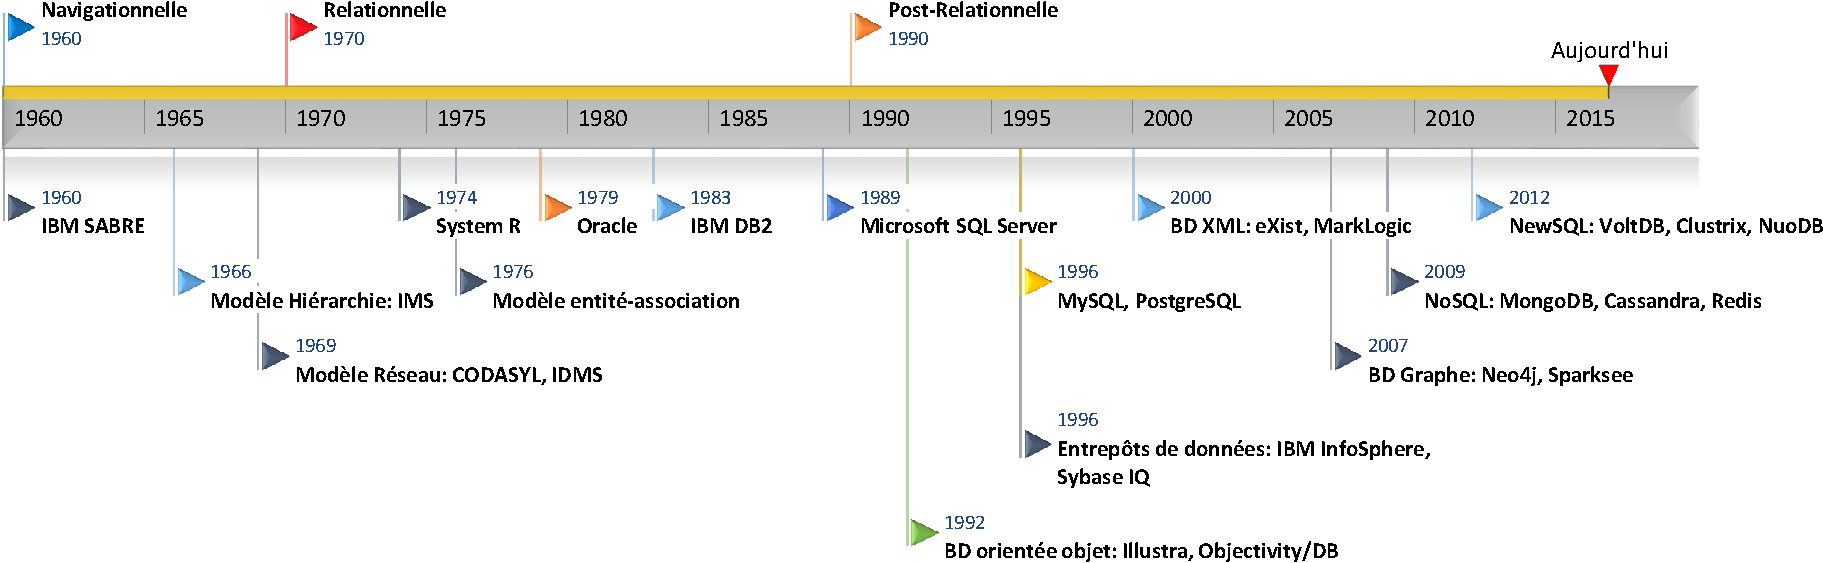
\includegraphics[scale=0.55]{chapitre2/chap2Fig/db-timeline.pdf}
\caption{Une brève évolution de la technologie des bases de données.}
 \label{fig:db-timeline}
\end{center}
\end{figure}

\subsection{Conception et cycle de vie}
% book: Database Systems - Design Implementation
% 1.4 WHY DATABASE DESIGN IS IMPORTANT

Une des tâches essentielles des développeurs de bases de données est la conception de leurs schémas. La conception de base de données est le processus de production d'un modèle de données détaillé de la base de données. Ce modèle de données contient tous les choix de conception logique et physique nécessaires et les paramètres de stockage physique nécessaires pour générer une conception dans un langage de définition de données, qui peut ensuite être utilisé pour créer une base de données. La représentation doit être juste pour éviter les erreurs sémantiques, notamment dans les réponses aux requêtes. Elle doit aussi être complète pour permettre le développement des programmes d’application souhaités. Elle doit enfin être évolutive afin de supporter la prise en compte rapide de nouvelles demandes \cite{Gardarin03}.

Une base de données bien conçue facilite la gestion des données et génère des informations précises et précieuses. Une base de données mal conçue est susceptible de devenir un terrain fertile pour les erreurs difficiles à tracer qui peuvent conduire à une mauvaise prise de décision et à l'échec d'une organisation. Même un bon SGBD fonctionnera mal avec une base de données mal conçue. La conception de base de données est tout simplement trop importante pour être laissée à la chance. L'objectif principal est de créer des modèles conceptuels, logiques et physiques complets, normalisés, non redondants et entièrement intégrés.

La création et l'évolution des bases de données suivent un schéma itératif appelé cycle de vie, un processus continu de création, de maintenance, d'amélioration et de remplacement des BDs. Traditionnellement, la démarche de conception et de cycle de vie d'une base de données s’effectue par des abstractions successives et itératives, en descendant depuis les problèmes de l’utilisateur vers la base de données finale \cite{Coronel09}. Nous proposons de distinguer cinq étapes :

% book: Physical Database Design
% 1.2 Database Life Cycle (p.26)
\begin{figure}
\begin{center}
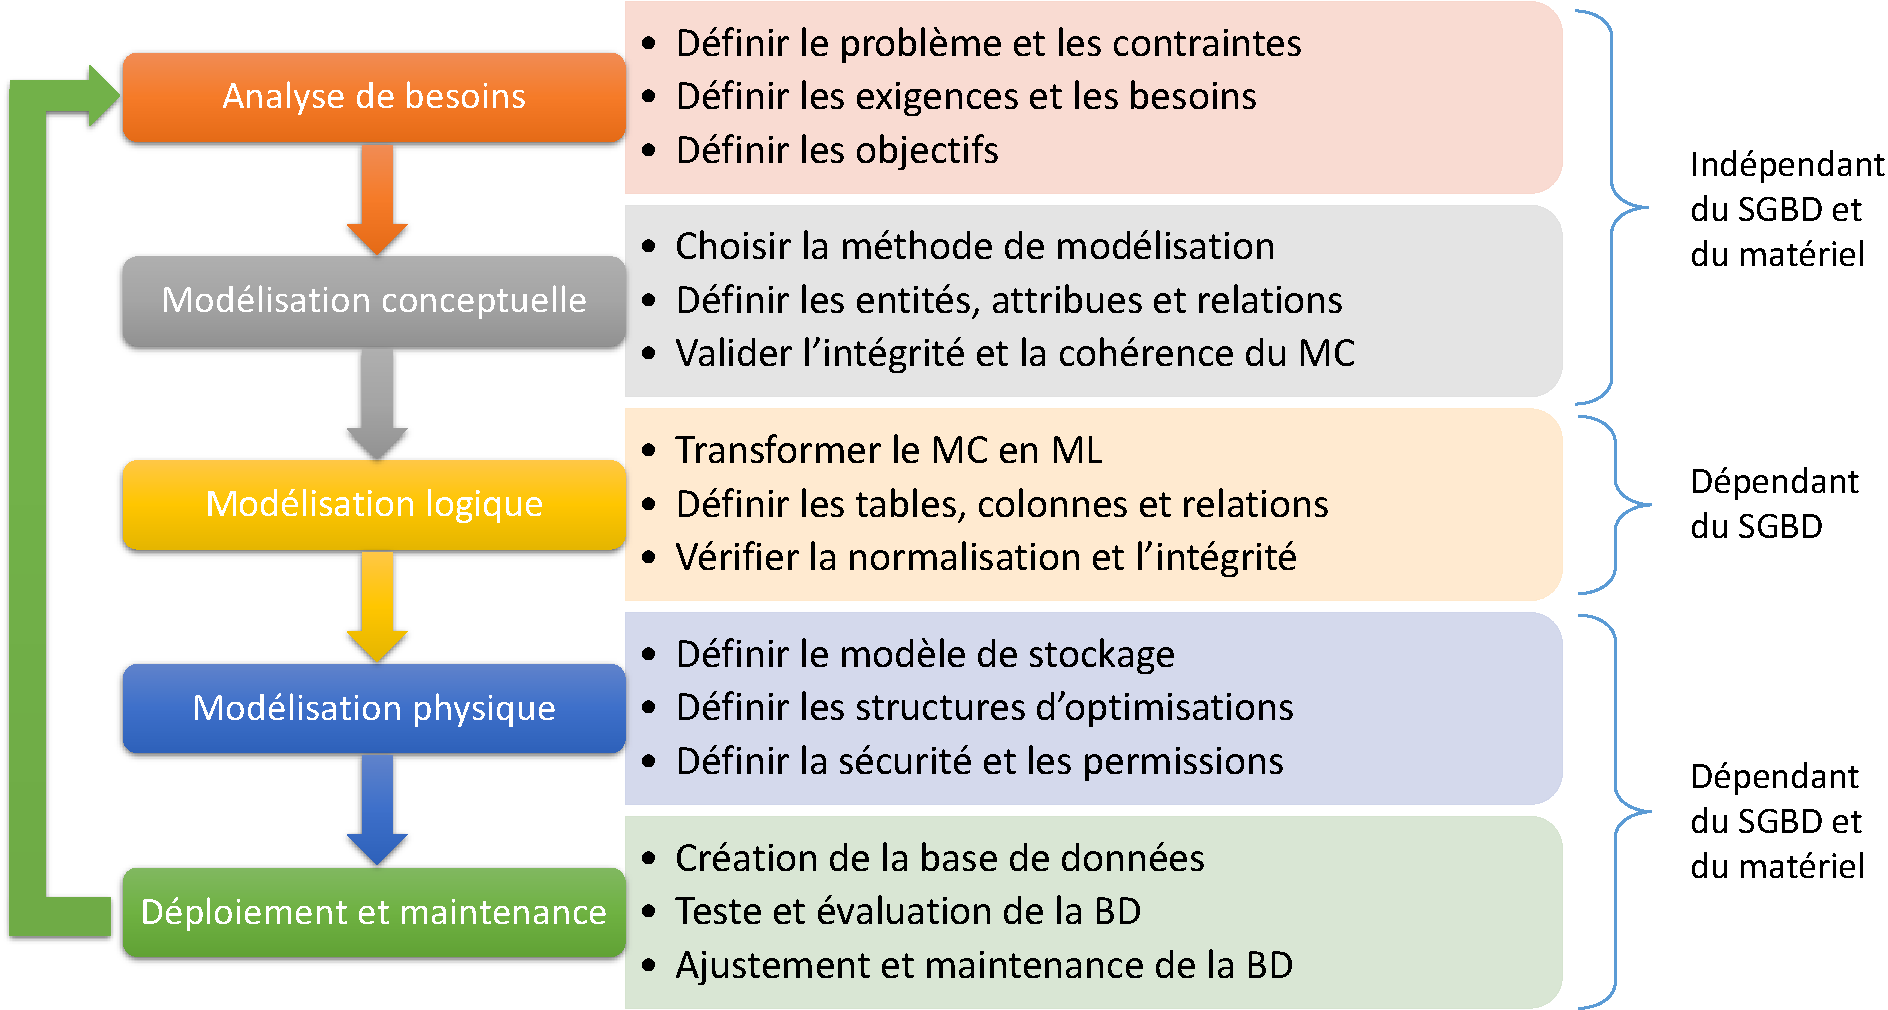
\includegraphics[scale=0.5]{chapitre2/chap2Fig/db-lifecycle.pdf}
\caption{Le cycle de vie des bases de données.}
 \label{fig:db-lifecycle}
\end{center}
\end{figure}

\begin{enumerate}
 \item \textbf{Analyse des besoins}. Consiste à définir et examiner les problèmes, les contraintes et les objectifs de l'entreprise. Une première évaluation des besoins et exigences, logiciels et matériels, relatives au flux d'information doit être effectuée lors de cette étape. La phase d'analyse du cycle de vie est, en fait, une vérification approfondie des besoins des utilisateurs. Le résultat est une spécification textuelle de ces besoins.
 \item \textbf{Modélisation conceptuelle}. L'objectif de cette étape est de concevoir une base de données indépendante du logiciel et des détails physiques de la base de données. La sortie de ce processus est un modèle de données conceptuelles qui décrit les principales entités de données, les attributs, les relations et les contraintes d'un domaine de problème donné. Cette conception est descriptive et narrative en forme. C'est-à-dire qu'elle est généralement composée d'une représentation graphique ainsi que de descriptions textuelles des principaux éléments de données, relations et contraintes. L'objectif est d'intégrer toutes les parties dans un schéma conceptuel global complet, non redondant et cohérent. Ce schéma global est développé en utilisant des techniques telles que la modélisation entité-association ou \gls{UML}.
 \item \textbf{Modélisation logique}. L'objectif de la modélisation logique est de concevoir une base de données à l'échelle de l'entreprise basée sur un modèle de données spécifique, mais indépendante des détails de niveau physique. La conception logique nécessite que tous les objets du modèle conceptuel soient mappés aux structures spécifiques utilisées par le modèle de base de données sélectionné. Par exemple, la conception logique d'un SGBD relationnel comprend les spécifications pour les relations (tables). Avec un SGBD objet, il s’agit de générer des classes et des associations. La conception logique ne doit contenir que des tables correctement normalisées et nécessite également la définition des domaines d'attributs et des contraintes appropriées.
 \item \textbf{Modélisation physique}. La modélisation ou conception physique est le processus de détermination de l'organisation du stockage de données et des caractéristiques d'accès aux données afin d'en assurer l'intégrité, la sécurité et les performances du système. Il s'agit de la dernière étape du processus de conception de base de données. Les caractéristiques de stockage sont déterminées en fonction des types de périphériques pris en charge par le matériel, du type de méthodes d'accès aux données prises en charge par le système et le SGBD. Dans cette étape, il faut choisir les bonnes structures d'optimisations physiques : vues matérialisées ou partitionnement de tables, index, etc. La conception physique pourrait devenir un travail très technique qui affecte non seulement l'accessibilité des données dans le(s) périphérique(s) de stockage, mais aussi la performance du système.
 \item \textbf{Déploiement et maintenance}. Le résultat des phases de conception de base de données est une série d'instructions détaillant la création de tables, d'attributs, d'index, de contraintes de sécurité, de règles de stockage, de performance, d'une architecture centralisée ou distribuée, etc. Dans cette phase, toutes ces spécifications de conception doivent être mises en œuvre. L'administrateur teste, évalue et ajuste la base de données pour s'assurer qu'elle fonctionne comme prévu. L'administrateur doit aussi effectuer des activités de maintenance dans la base de données. Certaines des activités de maintenance périodique comprennent la sauvegarde, la restauration, la modification des attributs et tables, génération de statistiques, audits de sécurité, etc.
\end{enumerate}

Le schéma illustré par la \ref{fig:db-lifecycle}, représente ce cycle de vie avec les tâches principales de chaque étape. Dans les sections suivantes nous détaillons ces différentes étapes en mettant l'accent sur la phase de conception physique.

\subsubsection{Analyse des besoins}
Dans le domaine de l'ingénierie logicielle, l'ingénierie des besoins est la branche du génie logiciel qui se consacre aux objectifs, aux fonctions et aux contraintes réels des systèmes logiciels. Elle s'intéresse également à la relation entre ces facteurs et les spécifications précises du comportement des logiciels, ainsi qu'à leur évolution dans le temps et dans les familles de logiciels \cite{Zave97}. Autrement dit, les besoins et les exigences des utilisateurs sont traduits en un ensemble de besoins qui définissent ce que le système doit faire et comment il doit le faire. Le concepteur de base de données doit s'assurer que les besoins sont compréhensibles, sans ambiguïté, complets et concis.
Les systèmes matériels et logiciels existants sont également étudiés pendant la phase d'analyse. Le résultat de l'analyse devrait être une meilleure compréhension des domaines fonctionnels du système et des problèmes actuels ou potentiels. Les utilisateurs finaux et le concepteur de systèmes doivent travailler ensemble pour identifier les processus et pour découvrir les zones à problèmes potentielles. Cette coopération est essentielle pour définir les objectifs de performance appropriés permettant de juger le nouveau système \cite{Coronel09}. Une bonne analyse des besoins est fondamentale pour une conception réussie de la base de données.
Les besoins se répartissent généralement en deux types: \textit{besoins fonctionnels} ($\mathcal{\acrshort[hyper=false]{BF}}$) et \textit{besoins non-fonctionnels} ($\mathcal{\acrshort[hyper=false]{BNF}}$) \cite{Zave97,Chung12,Ameller12}, tel que représenté dans la \ref{fig:reqs-classification}.

\paragraph{Besoin fonctionnel}
Le $\mathcal{BF}$ est défini comme étant tout besoin qui spécifie \textit{ce que} le système doit faire. En d'autres termes, un $\mathcal{BF}$ décrira un comportement particulier du fonctionnement du système lorsque certaines conditions sont valides, par exemple: << envoyer un courrier électronique lorsqu'un nouveau client s'inscrit >>. Des exemples des BFs dans une base de données incluent : gestion de transactions, authentification, niveaux d'autorisation, exigences de certification, données historiques, exigences légales ou réglementaires, etc.

\paragraph{Besoin non-fonctionnel}
Le $\mathcal{BNF}$ est défini comme étant tout besoin qui spécifie \textit{comment} le système effectue une certaine fonction. En d'autres termes, un $\mathcal{BNF}$ décrira comment un système doit se comporter et quelles limites il y a sur sa fonctionnalité. Les BNFs spécifient généralement les attributs ou caractéristiques de qualité du système, par exemple: << les données modifiées dans une base de données doivent être mises à jour pour tous les utilisateurs qui y accèdent en moins de 2 secondes >>. Par exemple, citons : performance, temps de réponse, consommation d'énergie,  évolutivité, disponibilité, fiabilité, la sécurité, utilisabilité, etc. Les BNFs sont généralement plus difficiles à analyser. En particulier, les BNFs ont tendance à être des propriétés d'un système dans son ensemble et ne peuvent donc pas être vérifiés pour des composants individuels \cite{Nuseibeh00}.

En outre, les BNFs peuvent être classés en deux catégories : $\mathcal{BNF}$ mesurable (BNFM) et $\mathcal{BNF}$ non-mesurable (BNFNM) \cite{Siegmund08}.

\subparagraph{BNFM}
Les BNFM sont des besoins qui peuvent être mesurés sur une échelle métrique définie par l'utilisateur. La métrique est définie par l'utilisateur car pour certains besoins, tel que la performance, il existe plusieurs métriques pour la quantifier. Les mesures peuvent être réalisées automatiquement par un ordinateur comme le temps de réponse, ou manuellement par un dispositif de mesure comme la consommation d'énergie.

\subparagraph{BNFNM}
Cette classe contient des besoins qui ne peuvent être décrits que qualitativement à l'aide d'une échelle ordinaire ou nominale, c'est-à-dire qu'il n'existe aucune métrique à partir de laquelle nous pouvons extraire des mesures quantifiables. Par exemple, considérer l'utilisabilité. Il faut réaliser de grandes études aux niveau des utilisateurs du système pour quantifier l'influence de différentes caractéristiques sur l'utilisabilité du système. L'évaluation d'une telle étude se fait d'habitude manuellement.

\begin{figure}
\footnotesize
\begin{center}
\tikzset{
  basic/.style  = {draw, text width=8em, drop shadow, rectangle},
  root/.style   = {basic, rounded corners=2pt, thin, align=center,
                   fill=green!30},
  level 1/.style = {basic, rounded corners=6pt, thin,align=center, fill=green!60,
                   text width=8em,sibling distance=55mm},
  level 2/.style = {basic, rounded corners=6pt, thin,align=center, fill=green!60,
                   text width=8em,sibling distance=40mm},
  level 3/.style = {basic, thin, align=left, fill=pink!60, text width=6.5em}
}
\begin{tikzpicture}[
  edge from parent/.style={->,draw,black},
  >=latex]

% root of the the initial tree, level 1
\node[root] {Types de besoins}
% The first level, as children of the initial tree
  child {node[level 1] (c1) {Fonctionnel}}
  child {node[level 1] (c2) {Non-fonctionnel}
	child {node[level 2] (c3) {Mesurable}}
	child {node[level 2] (c4) {Non-Mesurable}}
  };
  
\begin{scope}[every node/.style={level 3}]
\node [below of = c1, xshift=5pt] (c11) {Niveaux d'autorisations};
\node [below of = c11] (c12) {$\cdots$};
\node [below of = c3, xshift=5pt] (c31) {Performance};
\node [below of = c31] (c32) {$\cdots$};
\node [below of = c4, xshift=5pt] (c41) {Utilisabilité};
\node [below of = c41] (c42) {$\cdots$};
\end{scope}

\foreach \value in {1,...,2}
  \draw[->] (c1.178) |- (c1\value.west);
  
\foreach \value in {1,...,2}
  \draw[->] (c3.178) |- (c3\value.west);
  
\foreach \value in {1,...,2}
  \draw[->] (c4.178) |- (c4\value.west);

\end{tikzpicture}
\caption{Classification des types de besoins.}
\label{fig:reqs-classification}
\end{center}
\end{figure}

% book: Bases de données
% conception des bd p661
% 2. MODÉLISATION DES DONNÉES p15

% book: Database Systems - Design Implementation
% chapter 9: database design

% eBISS 2016
% 5 Audit of the DW Life Cycle
\subsubsection{Modélisation conceptuelle}
La modélisation conceptuelle consiste à créer un schéma conceptuel pour la base de données, à partir des besoins déjà collectés et analysés, en utilisant un modèle de données conceptuelles de haut niveau, tel que le modèle entité-association ou digramme de classe UML. Ce schéma représente les objets du monde réel de la manière la plus réaliste possible. Le modèle conceptuel doit comprendre une compréhension claire de l'entreprise et de ses $\mathcal{BF}$ et $\mathcal{BNF}$. À ce niveau d'abstraction, le type de matériel et/ou de SGBD à utiliser pourrait ne pas avoir été identifié. Par conséquent, la conception doit être indépendante du logiciel et du matériel afin que le système puisse être installé dans n'importe quelle plate-forme matérielle et logicielle choisie plus tard \cite{Coronel09}.

\begin{example}
 Une société spécialisée dans la vente souhaite dynamiser sa politique de vente en construisant un site web pour la vente de ses produits. Après l'étude des besoins de l'entreprise, le concepteur de BD a créé un schéma conceptuel avec le modèle entité-association. Voici la description de chaque entité :
 \begin{itemize}
  \item \textit{Clients} : Cette table conserve les informations sur les clients.
  \item \textit{Commandes} : Contient la liste des commandes des clients.
  \item \textit{Détail commandes} : Contient les informations détaillées sur les commandes.
  \item \textit{Produits} : Garde la liste des produits avec leur détaille.
  \item \textit{Stock} : Sauvegarde la quantité de chaque produit en stock.
 \end{itemize}
 Un exemple de schéma conceptuel défini en termes d'entités et d'associations entre ces entités est représenté dans la \ref{fig:conceptual-design-ex}.
\end{example}

\begin{figure}
\begin{center}
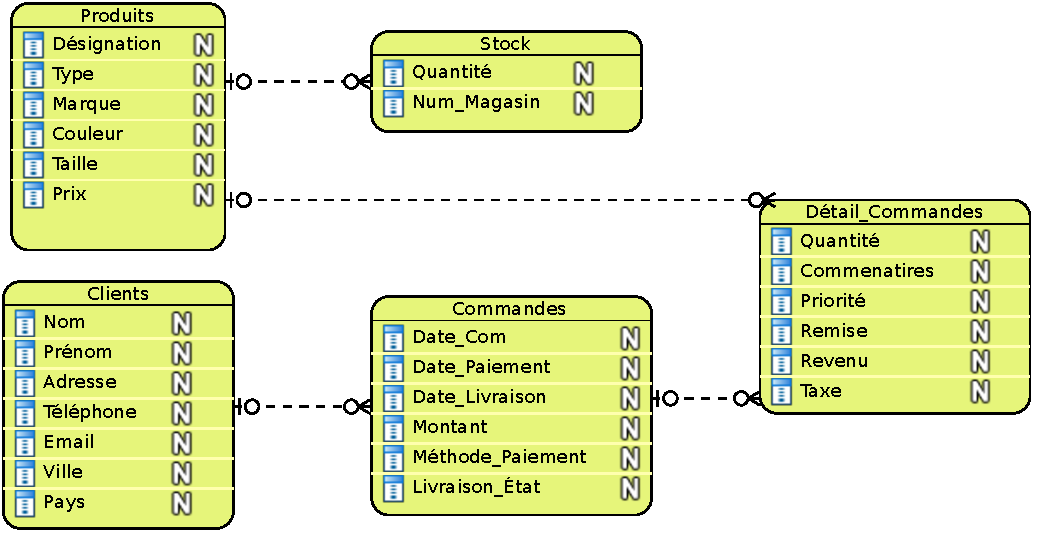
\includegraphics[scale=0.6]{chapitre2/chap2Fig/conceptual-design-ex.pdf}
\caption{Exemple d'un schéma de modélisation conceptuelle.}
\label{fig:conceptual-design-ex}
\end{center}
\end{figure}

\subsubsection{Modélisation logique}
La modélisation logique commence par le choix du SGBD suivant le modèle de données choisi dans l'étape précédente. Ensuite, le schéma conceptuel est transformé du modèle de données de haut niveau en modèle de données de mise en œuvre avec le SGBD \cite{Elmasri08}.
La création schéma logique peut se faire d'une manière automatisée. Il existe des règles sur la façon dont le modèle entité-association ou le diagramme de classe UML est transféré à des relations du schéma logique. Dans cette étape, les clés primaires et les clés étrangères sont définies.
La normalisation est la dernière partie de la conception logique. L'objectif de la normalisation est d'éliminer la redondance et les anomalies potentielles lors de la mise à jour. La redondance signifie que les mêmes données sont enregistrées plus d'une fois dans la base de données. L'anomalie de mise à jour est une conséquence de la redondance. Si une donnée est enregistrée en plusieurs endroits, les mêmes données doivent être mises à jour en plusieurs endroits. La normalisation est une technique par laquelle on peut modifier le schéma relationnel pour réduire la redondance \cite{Elmasri08}.

\begin{figure}
\begin{center}
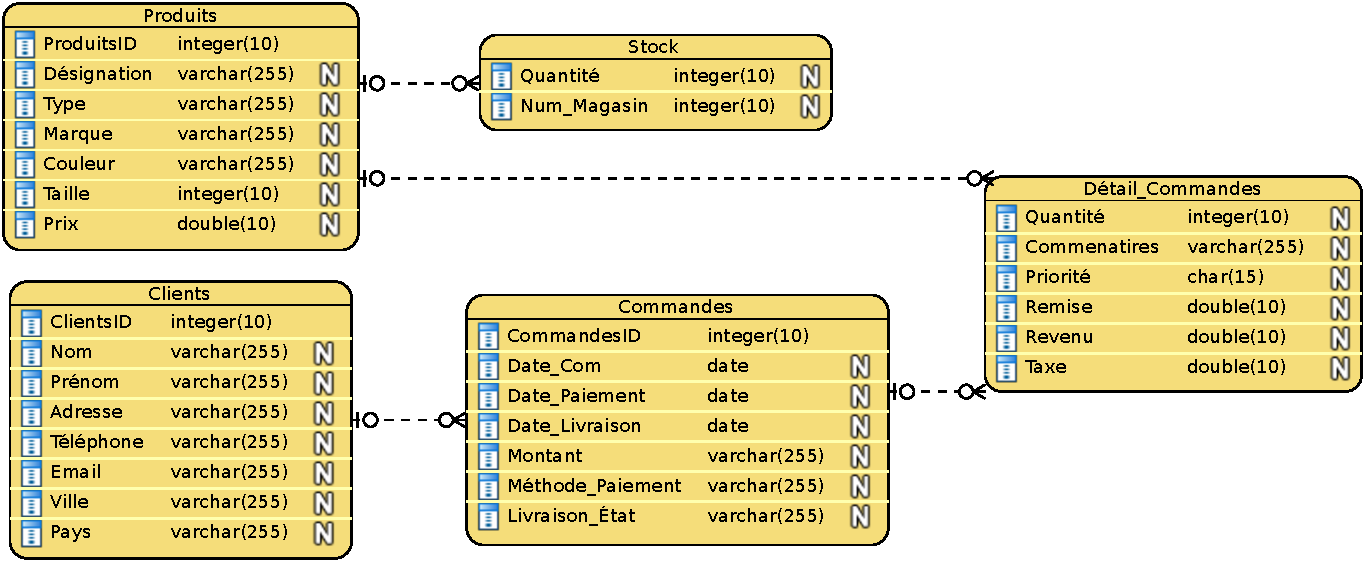
\includegraphics[scale=0.6]{chapitre2/chap2Fig/logical-design-ex.pdf}
\caption{Exemple d'un schéma de modélisation logique.}
\label{fig:logical-design-ex}
\end{center}
\end{figure}

\begin{example}
La \ref{fig:logical-design-ex} représente le schéma logique de notre exemple de gestion de vente. En peut remarquer que la définition des types de données des attributs et les clés primaires ont été établies sur les tables << \textit{Stock} >>, << \textit{Commandes} >> et << \textit{Clients} >>.
\end{example}

\subsubsection{Modélisation physique}
L'étape suivante est la conception physique, au cours de laquelle les structures de stockage internes, les organisations de fichiers, les indexes, les chemins d'accès, les contraintes d'intégrité, les droits d'accès des utilisateurs et les paramètres de conception physique des fichiers de base de données sont spécifiés \cite{Elmasri08}.

Dans cette étape, des structures d'optimisation ($\mathcal{\acrshort[hyper=false]{SO}}$) telles que les vues matérialisées, les indexes, le partitionnement de données, sont sélectionnées pour optimiser un ou plusieurs $\mathcal{BNF}$ tels que la performance des requêtes et l'énergie du système. La conception physique se concentre sur les méthodes de stockage et d'accès aux tables sur le disque qui permettent à la base de données de fonctionner avec une efficacité élevée. L'objectif est de maximiser les performances de la base de données sur l'ensemble du système. Les ressources physiques qui impliquent les performances lors de l'exécution des requêtes comprennent le CPU, les E/S (par exemple, les disques) et les connexions réseaux \cite{Lightstone10}.

\begin{example}
La \ref{fig:physical-design-ex} illustre le schéma physique de l'exemple précédent. Les informations ajoutées sont les clés étrangères sur les tables << \textit{Stock} >>, << \textit{Commandes} >> et << \textit{Détail\_Commandes} >>, et les indexes définis sur les tables << \textit{Clients} >> et << \textit{Produits} >> pour accélérer l'accès aux données de ces tables.\end{example}

\begin{figure}
\begin{center}
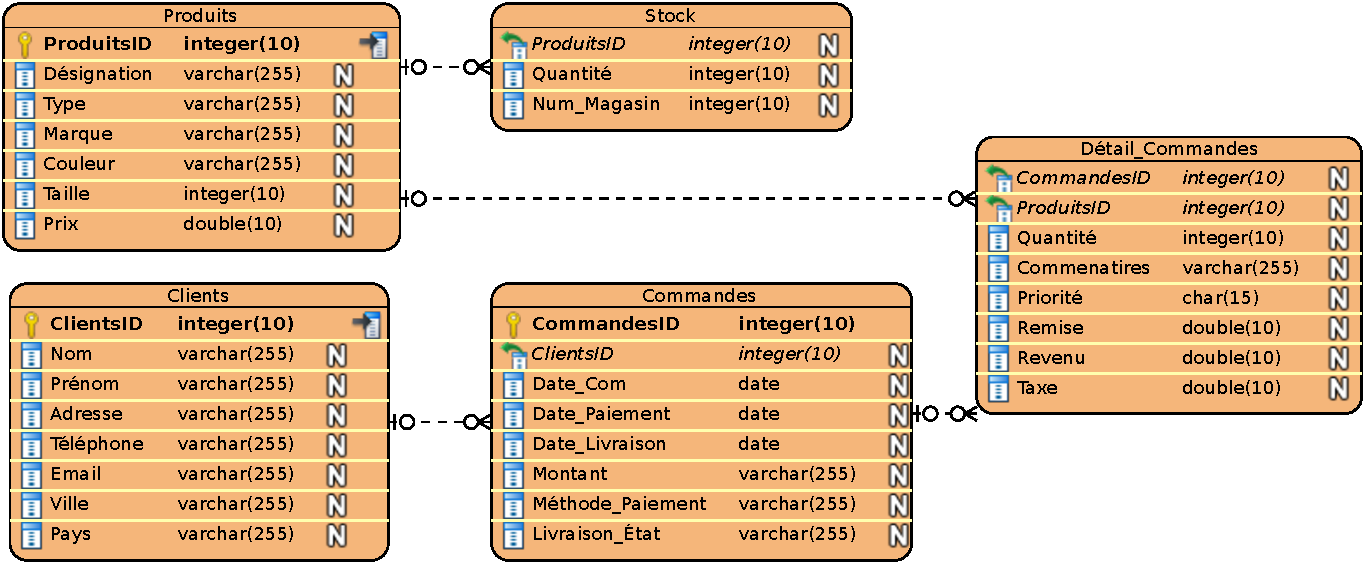
\includegraphics[scale=0.6]{chapitre2/chap2Fig/physical-design-ex.pdf}
\caption{Exemple d'un schéma de modélisation physique.}
\label{fig:physical-design-ex}
\end{center}
\end{figure}

Les optimisations physiques ont été amplifiées par l'explosion du volume des données et la nécessité d'optimiser ses modèles d'accès, ce qui est assuré par les $\mathcal{SO}$ \cite{ChaudhuriN07}. En exploitant les $\mathcal{SO}$, on peut réduire le temps de traitement des opérations dans certains cas de plusieurs ordres de grandeur. Une tâche critique pour l'administrateur de la base de données dans cette phase est le bon choix des $\mathcal{SO}$ pour satisfaire les $\mathcal{BNF}$ des utilisateurs. Cette tâche peut être divisée en quatre sous-tâches \cite{BellatrecheHdr09} :

\begin{enumerate}
 \item Le choix des structures d’optimisation : redondante ou non-redondante;
 \item Le choix du mode de sélection des structures d'optimisation : isolée ou multiple;
 \item Le choix et le développement des algorithmes de résolution;
 \item La validation et le déploiement des solutions d’optimisation.
\end{enumerate}

Dans ce suit, nous considérons le cas des vues matérialisées ($\mathcal{\acrshort[hyper=false]{VM}}$) qui est une $\mathcal{SO}$ redondante très utilisé dans les applications décisionnelles et les requêtes de type OLAP. 
% these kamel boukhelfa, ahcene
%\paragraph{Structure d'optimisation : Définition et classification}
\paragraph{Cas d'étude : Vues matérialisées}\label{sec:psv}
\begin{definition}
 Une vue est une relation logique qui utilise la définition de requête pour extraire les données à partir des tables correspondantes.
\end{definition}

\begin{definition}
 Une vue matérialisée est une table sur disque qui contient les résultats d'une requête. Elle peut s'agir d'une copie locale de données située à distance, ou un sous-ensemble des lignes et/ou colonnes d'un résultat de requête ou de jointure avec ou sans une fonction d'agrégation.
\end{definition}

Les $\mathcal{VM}$ sont de petites tailles par rapport à la table réelle et sont constituées de données importantes. Par conséquent, une exécution plus rapide des requêtes est possible. Lorsque les requêtes sont générées dans le système, les $\mathcal{VM}$ sont accédées en premier. Si les résultats ne sont pas trouvés dans les $\mathcal{VM}$, les tables réelles du système sont recherchées.

\begin{example}
Pour créer une vue matérialisée qui comptabilise la somme des ventes de chaque client par jour de notre base de données de vente, la requête SQL s'écrit comme suit :
	%\begin{verbatim}
	\begin{lstlisting}[language=Sql]
	CREATE MATERIALIZED VIEW resume_ventes AS
	SELECT Nom, Date_Com, SUM(Montant)
	FROM Clients Commandes
	WHERE Clients.ClientsID = Commandes.ClientsID
	GROUP BY Nom, Date_Com
	ORDER BY Nom, Date_Com;
    \end{lstlisting}
	%\end{verbatim}
Si la relation \textit{Commandes} contient des dizaines de millions de tuples, la différence entre le calcul de l'agrégation à partir des données de base et à l'aide de la vue matérialisée peut être de plusieurs ordres de grandeur.
\end{example}


Les défis à relever pour exploiter les vues matérialisées sont : (1) identifier les bonnes vues à matérialiser, (2) exploiter les $\mathcal{VM}$ pour répondre aux requêtes, et (3) mettre à jour efficacement les $\mathcal{VM}$ lors du changement des données de base \cite{Chaudhuri97b}.

\subparagraph{Problème de sélection des $\mathcal{VM}$}

L'administrateur de base de données ne peut pas matérialiser toutes les vues possibles, car il est limité par certaines ressources comme, l'espace disque et le temps de calcul, ceci est connu comme le problème de sélection des vues matérialisées ($\mathcal{\acrshort[hyper=false]{PSV}}$).
Le $\mathcal{PSV}$ consiste à trouver un ensemble approprié de vues satisfaisant un ensemble donné de $\mathcal{BNF}$ tels que la performance des requêtes, la fiabilité, l'utilisabilité, etc. Les $\mathcal{VM}$ sélectionnées doivent répondre à un ensemble de contraintes telles que le coût de stockage, les coûts de maintenance, etc. Le $\mathcal{PSV}$ est connu pour être un problème NP-complet \cite{Gupta99} en raison du fait que l'espace de solution s'accroît de façon exponentielle lorsque la taille du problème augmente. La formalisation générale de $\mathcal{PSV}$ est défini comme suit : Étant donné :

\begin{itemize}
\item un schéma d'une base de données : $DB$; 
\item une charge de requêtes : $\mathcal{W} = \{Q_1, Q_2, \cdots , Q_n\}$; 
\item un ensemble de contraintes : $\mathcal{C} = \{C_1, C_2, \cdots$ $ , C_p\}$; 
\item un ensemble de besoins non-fonctionnelles : $\mathcal{BNF} = \{nfr_1,$ $\cdots, nfr_k\}$. 
\end{itemize}

Le $\mathcal{PSV}$ consiste à sélectionner un ensemble de vues matérialisées : $MV = \{V_1, V_2, \cdots , V_m\}$ satisfaisant des $\mathcal{BNF}$ et en respectant l'ensemble des contraintes $\mathcal{C}$.

\begin{figure}
	\centering
	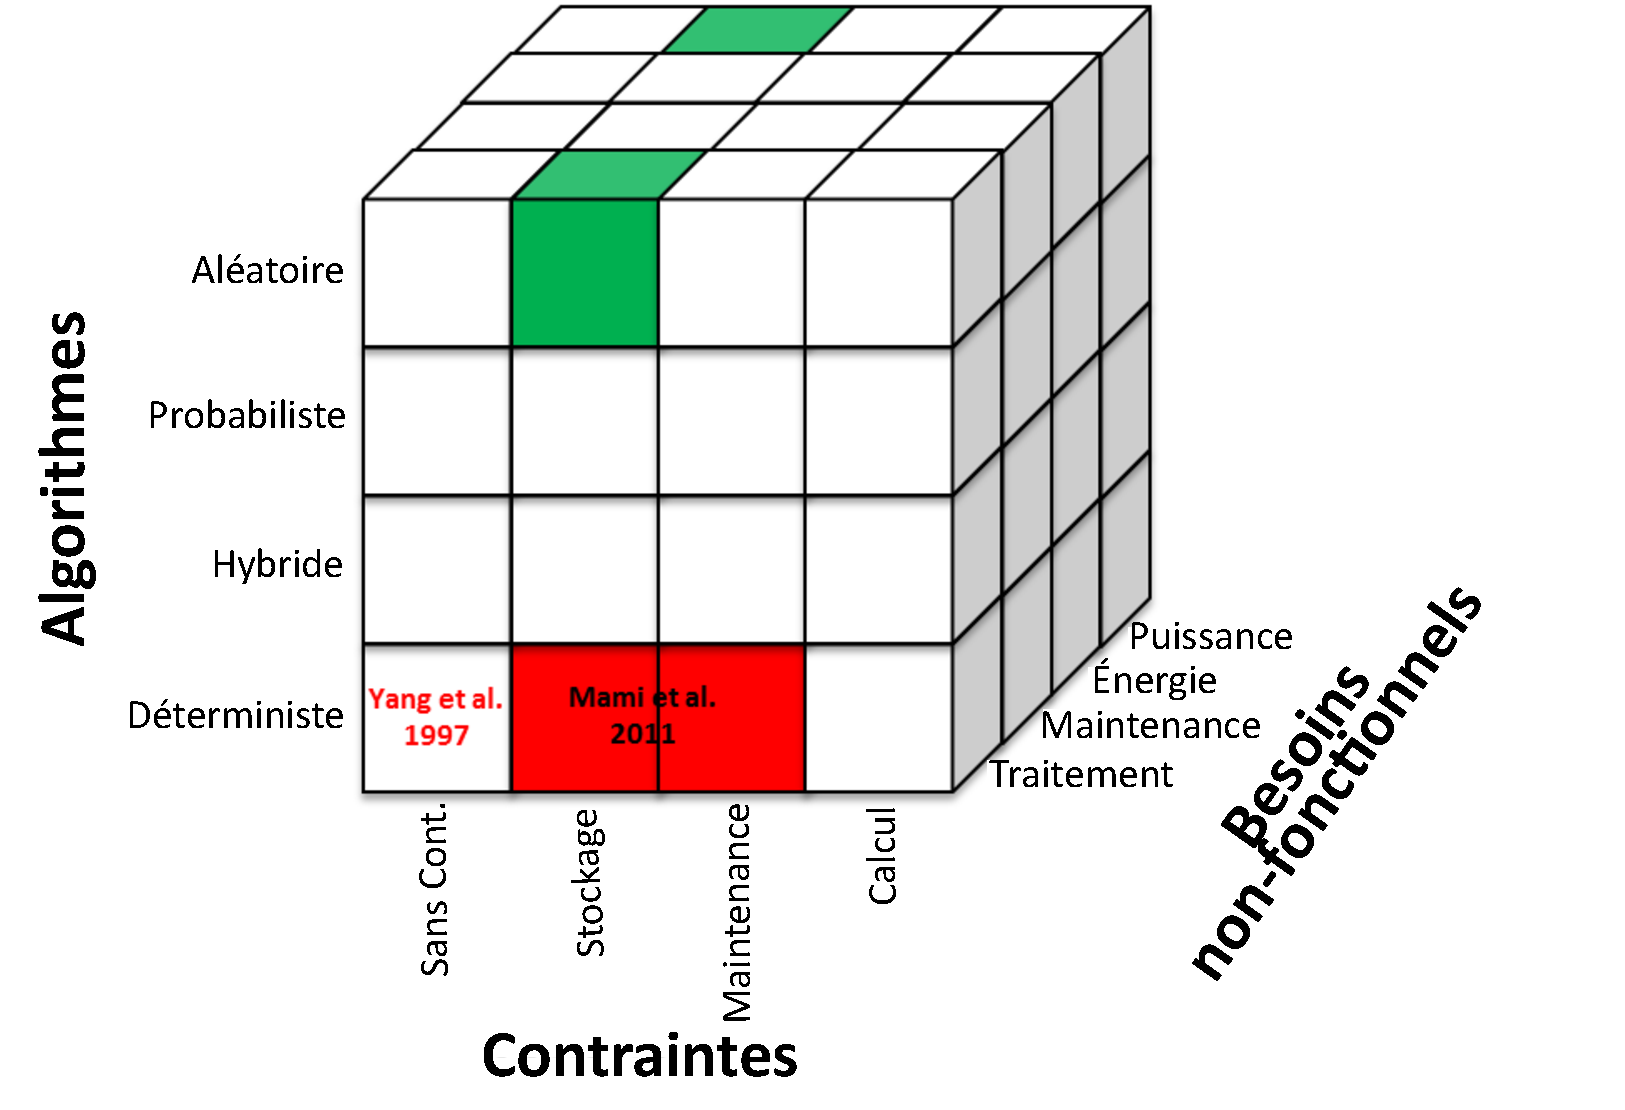
\includegraphics[scale=0.4]{chapitre2/chap2Fig/cubeNFR.pdf}
	\caption{Méthodes de résolutions du $\mathcal{PSV}$ .}
	\label{fig:warehouse-solutions}
\end{figure}

Plusieurs instanciations de cette formalisation existent. Nous proposons de les représenter par un \textit{cube} ayant trois dimensions principales : (i) le $\mathcal{BNF}$, (ii) les contraintes $\mathcal{C}$, et (iii) les algorithmes utilisés pour résoudre le $\mathcal{PSV}$. Ces dimensions permettent de classer les solutions existant dans l'état de l'art. La \ref{fig:warehouse-solutions} illustre notre cube.

\textbf{Les $\mathcal{BNF}$.} En ce qui concerne les $\mathcal{BNF}$ que les $\mathcal{VM}$ sélectionnés doivent satisfaire, elles couvrent plusieurs objectifs, tels que : la minimisation du temps de réponse des requêtes \cite{Ross96}, la minimisation du temps de réponse et du coût de maintenance \cite{Gupta97}. Ces objectifs peuvent être combinés pour donner lieu à une formalisation \textit{multi-objectif} du $\mathcal{PSV}$ comme dans \cite{Lawrence06} où le temps de réponse et le coût de maintenance ont été considérés.

\textbf{Les contraintes.} Les premières études sur le $\mathcal{PSV}$ supposent l'absence de contraintes \cite{Mistry01}. Par la suite et en raison de la grande taille de stockage des $\mathcal{VM}$ sélectionnées, l'espace de stockage devient la principale contrainte que le processus de sélection doit intégrer \cite{Gupta97}. Ensuite, le coût de maintenance devient un paramètre important car les $\mathcal{VM}$ sélectionnées doivent être mises à jour une fois les tables de base modifiées \cite{Gupta99}. Certaines études ont considéré les deux contraintes \cite{Kalnis02}. Récemment, des études traitent le cas du déploiement des $\mathcal{VM}$ dans un environnement distribué avec le coût de communication réseaux comme contrainte \cite{Chaves09,Mami16}, ou encore un environnement cloud sous la contrainte de coût monétaire \cite{Kehua14}. 

\textbf{Algorithmes de résolution.} 
La résolution de $\mathcal{PSV}$ est généralement réalisée soit par des algorithmes simples ou avancés qui couvrent des algorithmes \textit{déterministes} \cite{Gupta99,Gupta97,Boukorca15}, algorithmes \textit{aléatoires} \cite{Kalnis02,Lawrence06}, algorithmes \textit{hybrides} \cite{Zhang01}, et la \textit{programmation par contraintes} \cite{Mami11,Mami16} (pour plus de détails, voir l'étude de \cite{Mami12,Chirkova11}).

\textbf{Type de sélection.} Il existe deux approches pour la sélection des vues : \textit{statique} et \textit{dynamique}. Une approche de sélection de vue statique suppose que la charge de requêtes est fixe, et choisit ensuite l'ensemble de vues à matérialiser \cite{Yang97,Boukorca15}. Alors que, dans une approche de sélection de vue dynamique, la sélection est appliquée lorsqu'une requête arrive. Par conséquent, la charge de requêtes est construite progressivement et change avec le temps \cite{Kehua14,Kotidis99}.

\textbf{Structure de données.} Habituellement, la première étape dans la résolution de $\mathcal{PSV}$ est l'identification des vues candidates qui sont prometteuses pour la matérialisation. De nombreuses techniques de structures de données ont été proposées pour obtenir l'ensemble des vues candidates \cite{Mami12}:
\begin{itemize}
 \item \textbf{\textit{Graphe de vue ET/OU}} : est un graphe orienté acyclique (\acrshort[hyper=false]{DAG}), composé de deux types de nœuds : opération et équivalence. Chaque nœud d'opération correspond à une opération algébrique dans le plan d'une requête (sélection, jointure, projection, etc.). Chaque nœud d'équivalence correspond à un ensemble d'expressions logiques équivalentes. De nombreux algorithmes ont été proposés dans la littérature exploitant cette structure \cite{Gupta99,Gupta97,Mami11}. La \ref{fig:dag-andor-example} donne un exemple de graphe de vue ET/OU.
 \item \textbf{\textit{Traitement de plan multi-vue (\acrshort[hyper=false]{MVPP})}} : Le MVPP défini par Yang \textit{et al} \cite{Yang97} est un DAG dans lequel les nœuds racine sont les requêtes, les nœuds feuilles sont les relations de base et tous les autres nœuds intermédiaires sont des vues de sélection, de projection, de jointure ou d'agrégation qui contribuent à la construction d'une requête donnée \cite{Boukorca15,Zhang01}. Un exemple d'un MVPP est représenté sur la \ref{fig:dag-mvpp-example}.
 \item \textbf{\textit{Données cube treillis}} : est un DAG proposé dans le contexte des entrepôts de données multidimensionnel, dont les nœuds représentent les requêtes ou vues qui sont caractérisées par une opération de regroupement, et les arêtes définissent la relation entre les vues \cite{Kalnis02,Harinarayan96,Yu03}. La \ref{fig:dag-cubelattice-example} donne un exemple du graphe de treillis.
 \item \textbf{\textit{Transformation de requête}} : dans cette technique, le $\mathcal{PSV}$ prend comme entrer les définitions de requête. Le $\mathcal{PSV}$ est modélisé comme un problème de recherche d'espaces d'états en utilisant un ensemble de règles de transformation. Ces règles détectent et exploitent des sous-expressions communes entre les requêtes de la charge et garantissent que toutes les requêtes peuvent être répondu en utilisant exclusivement les $\mathcal{VM}$ \cite{Ligoudistianos98,Theodoratos97}.
 \item \textbf{\textit{Analyse syntaxique}} : cette technique analyse la charge de requêtes et sélectionne un sous-ensemble de relations à partir duquel on peut matérialiser une ou plusieurs vues, à condition de réduire le coût de la charge de requêtes de manière significative \cite{Agrawal00,Chaves09}.
\end{itemize}

\begin{figure}
  \centering
  \subfloat[Exemple d'un graphe de vue ET/OU.\label{fig:dag-andor-example}]{
    \resizebox{.3\textwidth}{!}{% \documentclass{standalone}
% \usepackage{tikz}
% \begin{document}
\begin{tikzpicture}[
every node/.style  = {fill=blue!20,draw=blue!50,thick,
	minimum size=1.5em,inner sep=0pt,font=\small},
circle_node/.style={circle},
rec_node/.style={rectangle},
edge from parent/.style={->,draw},
every label/.append style={font=\scriptsize},
>=latex]
  
    \node[rec_node] (r1) at (0, 0) {$R_1$};
    \node[rec_node] (r2) at (1, 0)  {$R_2$};
    \node[rec_node] (r3) at (2, 0) {$R_3$};
	\node[rec_node] (r4) at (3, 0) {$R_4$};
	\node[rec_node] (r5) at (4, 0) {$R_5$};
	\node[rec_node] (r6) at (5, 0) {$R_6$};
	\node[rec_node] (r7) at (6, 0) {$R_7$};
	
	\node[circle_node] (op1) at (0, 1) {$\sigma$};
	\node[circle_node] (op2) at (4, 1) {$\bowtie$};
	\node[circle_node] (op3) at (6, 1) {$\sigma$};
	
	\node[rec_node] (v3) at (0, 2) {$V_3$};
	\node[rec_node] (v4) at (4, 2) {$V_4$};
	\node[rec_node] (v5) at (6, 2) {$V_5$};
	
	\node[circle_node] (op4) at (1, 3) {$\pi$};
	\node[circle_node] (op5) at (3, 3) {$\pi$};
	\node[circle_node] (op6) at (5, 3) {$\pi$};
	
	\node[rec_node,label={\scriptsize $Q_1$}] (v1) at (2, 4) {$V_1$};
	\node[rec_node,label={\scriptsize $Q_2$}] (v2) at (4, 4) {$V_2$};


    \draw[->] (v1) -- (op4);
	\draw[->] (v1) -- (op5);
	\draw[->] (v2) -- (op5);
	\draw[->] (v2) -- (op6);
	
	\draw[->] (op4) -- (v3);
	\draw[->] (op4) -- (r2);
	\draw[->] (op5) -- (v4);
	\draw[->] (op5) -- (r3);
	\draw[->] (op6) -- (v5);
	\draw[->] (op6) -- (r6);
	
	\draw[->] (v3) -- (op1);
	\draw[->] (v4) -- (op2);
	\draw[->] (v5) -- (op3);
	
	\draw[->] (op1) -- (r1);
	\draw[->] (op2) -- (r4);
	\draw[->] (op2) -- (r5);
	\draw[->] (op3) -- (r7);
	
\end{tikzpicture}
%\end{document}
}
  }
  \quad
  \subfloat[Exemple d'un graphe de données cube treillis.\label{fig:dag-cubelattice-example}]{
    \resizebox{.15\textwidth}{!}{\begin{tikzpicture}[main_node/.style={circle,fill=blue!20,draw=blue!50,thick,
	minimum size=1.5em,inner sep=0pt,font=\small},
edge from parent/.style={->,draw},>=latex]
  
    \node[main_node,label={[shift={(0.5,-0.5)}]{\scriptsize 40}}] (1) at (0, 0) {$V_3$};
    \node[main_node,label={[shift={(0.5,-0.5)}]{\scriptsize 45}}] (2) at (1, 0)  {$V_4$};
    \node[main_node,label={[shift={(0.5,-0.5)}]{\scriptsize 50}}] (3) at (-1, 0) {$V_2$};
	\node[main_node,label={[shift={(0.5,-0.5)}]{\scriptsize 35}}] (4) at (0, -1) {$V_6$};
	\node[main_node,label={[shift={(0.5,-0.5)}]{\scriptsize 30}}] (5) at (1, -1) {$V_7$};
	\node[main_node,label={[shift={(0.5,-0.5)}]{\scriptsize 30}}] (6) at (-1, -1) {$V_5$};
	\node[main_node,label={[shift={(0.5,-0.5)}]{\scriptsize 100}}] (7) at (0, 1) {$V_1$};
	\node[main_node,label={[shift={(0.5,-0.5)}]{\scriptsize 1}}] (8) at (0, -2) {$_{null}$};

    \draw[->] (7) -- (3);
	\draw (7) edge[->] (2);
	\draw (3) edge[->] (4);
	\draw (2) edge[->] (4);
	
	\draw (1) edge[->] (6);
	\draw (1) edge[->] (5);
	\draw (6) edge[->] (8);
	\draw (5) edge[->] (8);
	
	\draw (7) edge[->] (1);
	\draw (3) edge[->] (6);
	\draw (4) edge[->] (8);
	\draw (2) edge[->] (5);
\end{tikzpicture}}
  }
  \quad
  \subfloat[Exemple d'un graphe de traitement de plan multi-vue.\label{fig:dag-mvpp-example}]{
    \resizebox{.35\textwidth}{!}{\begin{tikzpicture}[
every node/.style  = {fill=blue!20,draw=blue!50,thick,
	minimum size=1.5em,inner sep=0pt,font=\small},
circle_node/.style={circle},
rec_node/.style={rectangle},
edge from parent/.style={->,draw},
every label/.append style={font=\scriptsize},
>=latex]
  
    \node[rec_node] (r1) at (0, 0) {$R_1$};
    \node[rec_node] (r2) at (2, 0)  {$R_2$};
    \node[rec_node] (r3) at (4, 0) {$R_3$};
	\node[rec_node] (r4) at (6, 0) {$R_4$};
	
	\node[circle_node] (op1) at (0, 1) {$\sigma$};
	\node[circle_node] (op2) at (2, 1) {$\sigma$};
	\node[circle_node] (op3) at (4, 1) {$\sigma$};
	\node[circle_node] (op4) at (6, 1) {$\sigma$};
	
	\node[circle_node] (op5) at (1, 2) {$\sigma$};
	\node[circle_node] (op6) at (2.5, 1.7) {$\bowtie$};
	\node[circle_node] (op7) at (3.8, 2) {$\bowtie$};
	\node[circle_node] (op8) at (5, 2.2) {$\bowtie$};
	\node[circle_node] (op9) at (7, 2) {$\bowtie$};
	
	\node[circle_node] (op10) at (1, 3) {$\pi$};
	\node[circle_node] (op11) at (2.5, 3) {$\pi$};
	\node[circle_node] (op12) at (3.8, 3) {$\pi$};
	\node[circle_node] (op13) at (5, 3) {$\pi$};
	\node[circle_node] (op14) at (7, 3) {$\pi$};
	
	\node[circle_node] (q1) at (1, 4) {$Q_1$};
	\node[circle_node] (q2) at (2.5, 4) {$Q_2$};
	\node[circle_node] (q3) at (3.8, 4) {$Q_3$};
	\node[circle_node] (q4) at (5, 4) {$Q_4$};
	\node[circle_node] (q5) at (7, 4) {$Q_5$};

    \draw[->] (r1) -- (op1);
	\draw[->] (r2) -- (op2);
	\draw[->] (r3) -- (op3);
	\draw[->] (r4) -- (op4);
	
	\draw[->] (op1) -- (op5);
	\draw[->] (op1) -- (op6);
	\draw[->] (op2) -- (op5);
	\draw[->] (op2) -- (op6);
	\draw[->] (op3) -- (op7);
	\draw[->] (op3) -- (op9);
	\draw[->] (op4) -- (op8);
	\draw[->] (op4) -- (op9);
	
	\draw[->] (op5) -- (op10);
	\draw[->] (op6) -- (op11);
	\draw[->] (op6) -- (op7);
	\draw[->] (op7) -- (op12);
	\draw[->] (op7) -- (op8);
	\draw[->] (op8) -- (op13);
	\draw[->] (op9) -- (op14);
	
	\draw[->] (op10) -- (q1);
	\draw[->] (op11) -- (q2);
	\draw[->] (op12) -- (q3);
	\draw[->] (op13) -- (q4);
	\draw[->] (op14) -- (q5);
	
\end{tikzpicture}}
  }
  \caption{Des exemples de structures de données graphe orienté acyclique.}\label{fig:dag-examples}
\end{figure}

\subparagraph{Problème d'exploitation des $\mathcal{VM}$}
Le problème d'exploitation des $\mathcal{VM}$ est de trouver des méthodes efficaces pour répondre à une requête en utilisant un ensemble de $\mathcal{VM}$ précédemment définies sur la base de données, plutôt que d'accéder aux relations de base de données, afin d'améliorer le temps de traitement des requêtes \cite{Halevy01}. Cela se fait à l'aide de la \textit{réécriture de requête} : l'objectif est de trouver une réécriture équivalente de la requête originale en utilisant une ou plusieurs vues. Ce problème est prouvé NP-complet \cite{Levy95}.

Les approches proposées dans la littérature pour résoudre ce problème se basent sur l'adaptation du modèle de coût de l'optimiseur de requêtes afin de générer le meilleur plan équivalant. Les travaux peuvent être classés en algorithmes de style \textit{System-R} et en algorithmes de \textit{transformation}. Les travaux initiaux ont incorporé des vues dans l'énumération de jointure d'un optimiseur de style System-R \cite{Chaudhuri95,Levy95}. Tandis que les travaux ultérieurs qui traitent un ensemble d'opérateurs SQL plus étendu ont utilisé des règles de transformation \cite{Goldstein01,Zaharioudakis00}.

\subparagraph{Problème de maintenance des $\mathcal{VM}$}
Lorsqu'une relation de base (table) est modifiée, les $\mathcal{VM}$ construites sur celle-ci doivent être mises à jour afin de produire des résultats de requêtes à jour. Le processus de mise à jour d'une vue matérialisée est connu sous le nom de \textit{maintenance de vue}. Les approches de maintenance des vues peuvent être classées en trois catégories : (1) la maintenance de vue basique par le \textit{recalcule} des vues depuis le début \cite{Gupta95}, (2) la maintenance de vue \textit{incrémentale}, où seules les modifications des vues matérialisées sont calculées \cite{Mohania97}, et (3) \textit{l'auto-maintenance} qui est un processus de rafraîchissement de vues progressif sans examiner aucune des relations de base \cite{Gupta95b}.

\begin{figure}
\footnotesize
\begin{center}
% \documentclass{standalone}
% \usepackage[utf8]{inputenc}
% \usepackage[T1]{fontenc}
% \usepackage{tikz}
% \usetikzlibrary{arrows,shapes,positioning,shadows,trees}
% 
% \begin{document}
\begin{tikzpicture}
\tikzset{
	grow cyclic,
text width=2.7cm, align=flush center,
  basic/.style  = {draw, text width=2.7cm, drop shadow, rectangle},
  root/.style   = {basic, rounded corners=2pt, thin, align=center,fill=green!30},
%   level 1/.style = {basic, rounded corners=6pt, thin,align=center, fill=green!60,
%                    text width=6em,font=\footnotesize},
%   level 2/.style = {basic, thin, align=left, fill=pink!60, text width=6em,font=\scriptsize}
level 1/.style={level distance=3.5cm,sibling angle=50,
	basic, rounded corners=6pt, thin,align=center, fill=green!60, font=\footnotesize},
level 2/.style={text width=2cm, font=\footnotesize, level distance=3.5cm,sibling angle=30,
	basic, thin, align=left, fill=pink!60},
edge from parent/.style={->,draw,black},
>=latex
}
[]
\node[root] {Technique de $\mathcal{VM}$}
  child {node[level 1]{$\mathcal{BNF}$}
	child {node[level 2]{Temps de réponse \cite{Ross96}}}
	child {node[level 2]{Maintenance \cite{Gupta97}}}
	child {node[level 2]{Multi-objectif \cite{Lawrence06}}}
  }
  child {node[level 1]{Stratégie de maintenance}
    child {node[level 2, xshift=-10pt,yshift=10pt]{Recalcul \cite{Gupta95}}}
    child {node[level 2, xshift=-20pt]{Incrémentale \cite{Mohania97}}}
    child {node[level 2, xshift=15pt]{Auto-maintenance \cite{Gupta95b}}}
  }
  child {node[level 1, xshift=7pt, yshift=20pt]{Algorithmes de résolution}
	child {node[level 2]{Déterministes \cite{Gupta99,Gupta97,Boukorca15}}}
    child {node[level 2, yshift=18pt]{Aléatoires \cite{Kalnis02,Lawrence06}}}
    child {node[level 2, yshift=8pt]{Hybrides \cite{Zhang01}}}
    child {node[level 2]{Programmation par contraintes \cite{Mami11,Mami16}}}
  }
  child {node[level 1]{Type de sélection}
    child {node[level 2]{Statique \cite{Yang97,Boukorca15}}}
    child {node[level 2]{Dynamique \cite{Kehua14,Kotidis99}}}
  }
  child {node[level 1]{Structures de données}
    child {node[level 2]{Graphe ET/OU \cite{Gupta99,Gupta97,Mami11}}}
    child {node[level 2]{MVPP \cite{Yang97,Boukorca15,Zhang01}}}
    child {node[level 2]{Treillis \cite{Kalnis02,Harinarayan96,Yu03}}}
    child {node[level 2, yshift=10pt]{Transformation de requêtes \cite{Ligoudistianos98,Theodoratos97}}}
    child {node[level 2, yshift=-20pt]{Analyse syntaxique \cite{Agrawal00,Chaves09}}}
  }
  child {node[level 1]{Réécriture de requêtes}
    child {node[level 2, yshift=20pt]{System-R \cite{Chaudhuri95,Levy95}}}
    child {node[level 2]{Transformation \cite{Goldstein01,Zaharioudakis00}}}
  }
  child {node[level 1]{Contraintes}
    child {node[level 2]{Aucune \cite{Mistry01}}}
    child {node[level 2, yshift=-10pt]{Stockage \cite{Gupta97}}}
    child {node[level 2]{Maintenance \cite{Gupta99}}}
    child {node[level 2]{Réseaux \cite{Chaves09,Mami16}}}
    child {node[level 2]{Monétaire \cite{Kehua14}}}
  };
\end{tikzpicture}
% \end{document}
\caption{Classification des travaux pour la technique de $\mathcal{VM}$.}
\label{fig:mv-classification}
\end{center}
\end{figure}

Sur la base des travaux présentés dans cette section, nous proposons une classification qui incluent de nouvelles dimensions telles que les techniques de réécriture de requêtes, la stratégie de maintenance des $\mathcal{VM}$. La \ref{fig:mv-classification} illustre cette classification.

\subsubsection{Déploiement et maintenance}
Une fois la conception logique et physique terminée, la base de données peut être créée et déployée grâce à la mise en œuvre des schémas précédents. Cette phase consiste à choisir la plate-forme adéquate dans laquelle la base de données cible sera déployée. Plusieurs plates-formes peuvent stocker la base de données : machines centralisées, décentralisées, parallèles, cloud, etc. Le choix de la plate-forme de déploiement dépend du budget de l'entreprise et des $\mathcal{BNF}$ fixés \cite{Coronel09}.

Lorsque la base de données est mise en marche, la surveillance indique si les $\mathcal{BF}$ et $\mathcal{BNF}$ sont respectées. Si elles ne sont pas satisfaites, des modifications ou \textit{tuning} doivent être apportées pour améliorer les performances. D'autres modifications peuvent être nécessaires lorsque les besoins changent ou la quantité de données évolue \cite{Lightstone10}. Ainsi, le cycle de vie se poursuit avec la surveillance, le tuning et les modifications.

% TODO: Vers l'intégration de l'énergie dans le cycle de vie de la base de données
\subsubsection{Bilan et discussion}
Dans les sections précédentes, nous avons présenté et étudié le cycle de vie de la conception des bases de données. Cette étude nous permet de comprendre les différentes caractéristiques de chaque phase et les interdépendances qui peuvent exister entre elles. L'étude contribue également à identifier les phases potentielles pour intégrer la dimension de l'énergie. Nous pouvons constaté que l'énergie est influencée par toutes les étapes du cycle : (1) l'énergie est considérée comme un nouveau $\mathcal{BNF}$ dans une entreprise qui veut créer/modifier sa base de données à fin de minimiser la consommation d'énergie du système, (2) le choix du modèle conceptuel (entité-association ou UML par exemple) influence aussi sur les étapes suivantes du cycle et modifie par conséquent le comportement de l'énergie du système, (3) le choix du type du SGBD lors de la modélisation logique a un impact majeur sur la consommation de l'énergie car il est responsable de la gestion des données et sa structure interne diffère d'un SGBD à un autre (par exemple un SGBD orienté colonne améliore la performance et peut influencer sur l'énergie), (4) la conception physique influe largement sur l'énergie, l'organisation physique des données, les méthode d'accès, le choix des $\mathcal{SO}$ ont tous un effet sur l'usage de l'énergie, (4) finalement, le choix de l'environnement de déploiement de la base de données (centralisé, distribué, etc.) rend l'amélioration de l'efficacité énergétique un processus non trivial.

Notez que le choix approprié de la variante d'une technique de conception donnée dans chaque phase est crucial, et peut avoir un effet sur les autres phases et sur l'énergie globale du système. En résumé, nous concluons que chaque phase du cycle de vie de la conception des bases de données devrait être intégrée à la conception de systèmes de bases de données éco-énergétiques.

\subsection{Traitement de requêtes dans un SGBD relationnel}
% Book: Physical Database Design: the database professional's guide to exploiting indexes, views, storage, and more
% 3 Query Optimization and Plan Selection 31
% 11 Query Execution Plans and Physical Design 197

% book: Database Systems - Design Implementation
% 11.2 QUERY PROCESSING

% book: base de données
% chapitre x: optimisation des questions p301

Après la conception et la création de la base de données, les utilisateurs peuvent exploiter les données. Le traitement de requêtes est le groupe de composants d’un SGBD qui transforme les requêtes des utilisateurs et les commandes de modification des données en une séquence d’opérations de base de données et exécute ces opérations \cite{GarciaMolina08}. Notre but est d'examiner le processus de traitement de requêtes dans un SGBD pour des opportunités de minimisation d'énergie.

Dans ce chapitre, nous discuterons des techniques utilisées en interne par un SGBD pour traiter des requêtes de haut niveau. Une requête exprimée dans un langage de requête de haut niveau comme SQL doit d'abord être analysée syntaxiquement. \textit{L'analyseur} identifie les mots clés de la requête (les mots clés SQL, les noms d'attributs et les noms de relations) qui apparaissent dans le texte de la requête, et vérifie la syntaxe de requête pour déterminer si elle est formulée selon les règles de syntaxe (règles de grammaire) du langage de requête. La requête doit également être \textit{validée} en vérifiant que tous les noms d'attributs et de relations sont des noms valides et sémantiquement significatifs dans le schéma de la base de données. En utilisant des règles de \textit{transformation}, une représentation interne de la requête est ensuite créée, habituellement sous la forme d'une structure de données arborescente appelée \textit{arbre algébrique}. Le SGBD doit alors concevoir une stratégie \textit{d'exécution} ou un \textit{plan de requête} pour extraire les résultats de la requête à partir des fichiers de base de données. Une requête a de nombreuses stratégies d'exécution possibles, et le processus de choisir un approprié pour traiter une requête est connu sous le nom \textit{d'optimisation de requête} \cite{Elmasri08}. La \ref{fig:query-processing} donne un aperçu du processus de traitement des requêtes par un SGBD.

% TODO: add more references in each section !!

\begin{figure}
\begin{center}
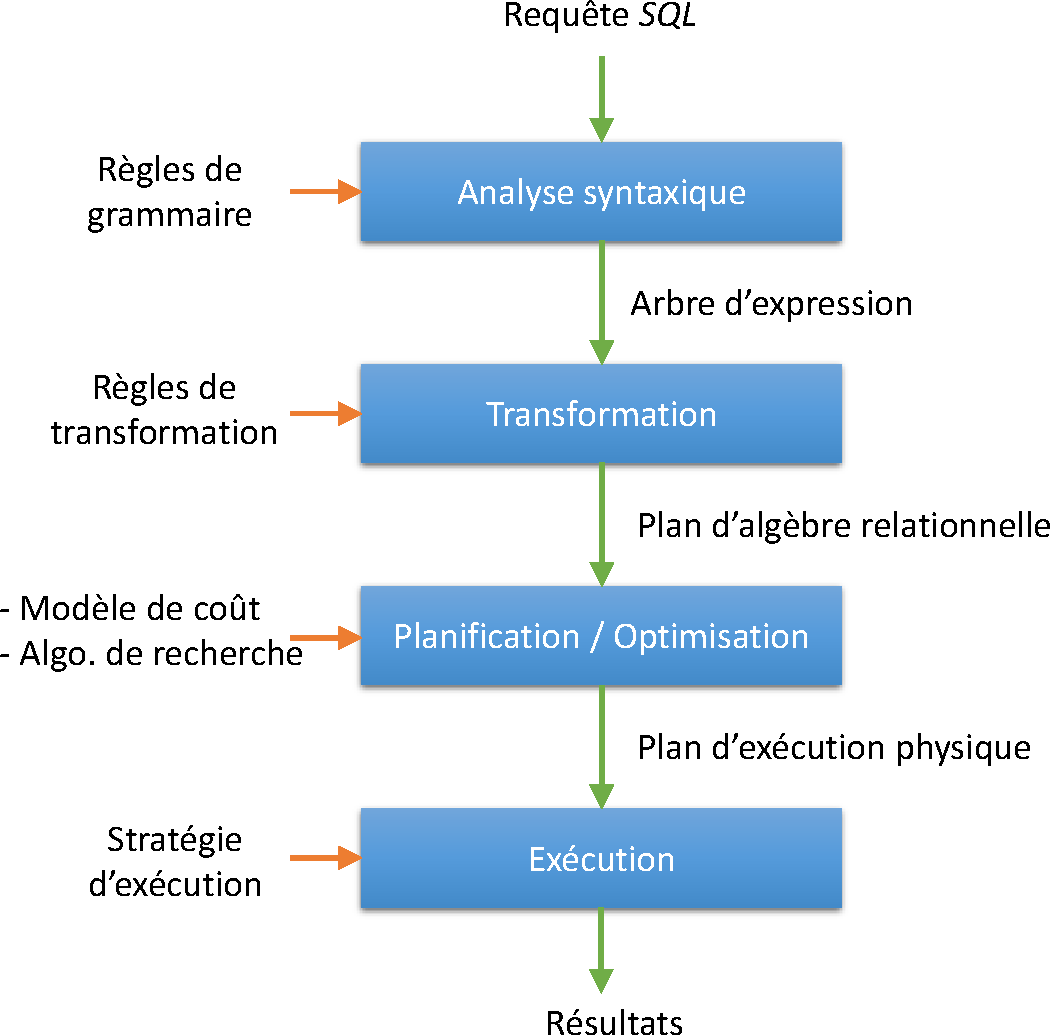
\includegraphics[scale=0.55]{chapitre2/chap2Fig/query-processing.pdf}
\caption{Architecture globale pour le traitement de requêtes dans un SGBD.}
 \label{fig:query-processing}
\end{center}
\end{figure}

\subsubsection{Analyse}
Le travail de l'analyseur est de prendre du texte écrit dans une langue comme SQL et de le convertir en un arbre d'analyse, qui est un arbre dont les nœuds correspondent soit à : (1) \textit{atomes}, qui sont des éléments lexicaux tels que des mots clés (par exemple, \texttt{SELECT}), des noms d'attributs ou de relations, des constantes, des parenthèses, des opérateurs tels que \texttt{+} ou \texttt{<}, et d'autres éléments de schéma, ou (2) des \textit{catégories syntaxiques}, qui sont des noms pour des sous-parties de requête qui ont un rôle similaire. Ils sont représentés par un nom descriptif entre les symboles \texttt{<} et \texttt{>} \cite{GarciaMolina08}. Par exemple, \texttt{<Requête>} est utilisé pour représenter une requête, et \texttt{<Condition>} représentera toute expression qui est une condition. Nous présenterons ces propos par un exemple dans la section suivante.

\paragraph{Une grammaire pour un sous-ensemble simple de SQL}
Nous allons illustrer le processus d'analyse en donnant quelques règles qui décrivent un petit sous-ensemble de requêtes SQL.

\subparagraph{Requête}
La catégorie syntaxique <Requête> est destinée à représenter certaines requêtes SQL. Nous lui donnons la règle :
\begin{verbatim}
<Requête> ::= SELECT <Sélection> FROM <Depuis> WHERE <Condition>
\end{verbatim}

Le symbole \microtypesetup{kerning=false}\texttt{::=}\microtypesetup{kerning=true} signifie << peut-être exprimer comme >>. Les catégories syntaxiques \texttt{<Sélection>}, \texttt{<Depuis>} et \texttt{<Condition>} représentent des listes pouvant suivre \texttt{SELECT}, \texttt{FROM} et \texttt{WHERE}, respectivement. Nous décrirons les formes de ces listes dans les prochaines sections.

\subparagraph{Sélection}
\begin{verbatim}
<Sélection> ::= <Attribut>, <Sélection>
<Sélection> ::= <Attribut>
\end{verbatim} 
Ces deux règles disent qu'une liste de sélection peut être une liste d'attributs séparés par des virgules : soit un attribut unique, soit un attribut, une virgule et toute liste d'un ou plusieurs attributs.

\subparagraph{Depuis}
\begin{verbatim}
<Depuis> ::= <Relation>, <Depuis>
<Depuis> ::= <Relation>
\end{verbatim}
Ici, une liste de type \texttt{Depuis} est définie comme étant une liste de relations séparées par des virgules.

\subparagraph{Condition}
Les règles que nous utiliserons sont :
\begin{verbatim}
<Condition> ::= <Condition> AND <Condition>
<Condition> ::= <Attribut> IN ( <Requête> )
<Condition> ::= <Attribut> = <Attribut>
<Condition> ::= <Attribut> LIKE <Motif>
\end{verbatim}

\subparagraph{Catégories syntaxiques}
Les catégories syntaxiques \texttt{<Attribut>}, \texttt{<Relation>} et \texttt{<Motif>} sont spéciales, puisqu'elles ne sont pas définies par des règles grammaticales, mais par des règles sur les atomes pour lesquels elles peuvent être utilisées. Par exemple, dans un arbre d'analyse, l'un des fils de \texttt{<Attribut>} peut être n'importe quelle chaîne de caractères qui identifie un attribut du schéma de base de données. De même, \texttt{<Relation>} peut être remplacé par n'importe quelle chaîne de caractères qui représente une relation dans le schéma, et \texttt{<Motif>} peut être remplacé par n'importe quelle chaîne entre guillemets qui est un modèle SQL légal.

\begin{example}\label{ex:parser-tree}
Notre étude de l'analyse et de la réécriture de requêtes sera basée sur notre exemple de gestion de vente. Nous voulons répondre à la requête << trouver les noms des clients qui ont payé leurs commandes en espèces >>. Nous identifions les clients qui ont payé des commandes en espèces en demandant si leur méthode de paiement est égale à << espèces >>, en utilisant l'opérateur \texttt{=}.
\end{example}

La requête SQL utilisé pour réponde à cette question est :
% \begin{verbatim}
% SELECT Nom
% FROM Clients, Commandes
% WHERE Clients.ClientsID = Commandes.ClientsID AND
%       Méthode_Paiement = 'espèces';
% \end{verbatim}
\begin{lstlisting}[language=Sql]
SELECT Nom
FROM Clients, Commandes
WHERE Clients.ClientsID = Commandes.ClientsID AND
      Méthode_Paiement = 'espèces';
\end{lstlisting}

L'arbre d'analyse pour notre requête, selon la grammaire que nous avons proposée, est illustré dans la \ref{fig:parser-tree}. A la racine se trouve la catégorie syntaxique \texttt{<Requête>}. En parcourant l'arbre, nous voyons que cette requête a une forme de \texttt{select-from-where}, la liste de \texttt{<Sélection>} se compose uniquement de l'attribut \texttt{Nom} et la liste de \texttt{<Depuis>} contient plus d'une relation et deux conditions connectées par \texttt{AND}.

\begin{figure}
\scriptsize
\begin{center}
\tikzset{>=latex}

\begin{forest} for tree={align=center}
[<Requête>
    [\texttt{SELECT}]
    [<Sélection>
        [<Attribut>
            [\texttt{Nom}]
        ]
    ]
    [\texttt{FROM}]
    [<Depuis>
		[<Relation>
			[\texttt{Clients}]
		]
		[\texttt{,}]
		[<Depuis>
			[<Relation>
				[\texttt{Commandes}]
			]
		]
    ]
    [\texttt{WHERE}]
    [<Condition>
		[<Condition>
			[<Attribut>
				[\texttt{ClientsID}]
			]
			[\texttt{=}]
			[<Attribut>
				[\texttt{ClientsID}]
			]
		]
		[\texttt{AND}]
		[<Condition>
			[<Attribut>
				[\texttt{Méthode\_Paiement}]
			]
			[\texttt{=}]
			[<Attribut>
				[\texttt{'espèces'}]
			]
		]
	]
]
\end{forest}
\caption{Exemple d'un arbre d'analyse.}
\label{fig:parser-tree}
\end{center}
\end{figure}

L'analyseur vérifie si une relation dans la requête est en réalité une vue virtuelle, chaque utilisation de cette relation dans la requête doit être remplacée par un arbre d'analyse qui décrit la vue \cite{GarciaMolina08}.
L'analyseur est aussi responsable de la vérification sémantique. Même si la requête est valable syntaxiquement, elle peut en fait violer une ou plusieurs règles sémantiques sur l'utilisation des noms. Par exemple, l'analyseur doit :

\begin{itemize}
 \item \textit{Vérifiez les relations} : Chaque relation mentionnée dans une clause \texttt{FROM} doit être une relation ou une vue dans le schéma de la base de données courante.
 \item \textit{Vérifiez et résoudre les attributs} : Chaque attribut mentionné dans la clause \texttt{SELECT} ou \texttt{WHERE} doit être un attribut d'une certaine relation dans la requête. Par exemple, l'attribut \texttt{Nom} est un attribut de \texttt{Clients}, donc l'analyseur valide cette utilisation. Il vérifie également l'ambiguïté, signalant une erreur si un attribut est dans la portée de deux ou plusieurs relations.
 \item \textit{Vérifiez les types} : Tous les attributs doivent être d'un type approprié à leurs utilisations. Par exemple, \texttt{Méthode\_Paiement} est utilisé dans une comparaison \texttt{=}, ce qui nécessite que cet attribut soit une chaîne ou un type qui peut être contraint à une chaîne. De même, les opérateurs sont vérifiés pour voir qu'ils s'appliquent aux valeurs des types appropriés et compatibles.
\end{itemize}

\subsubsection{Transformation}\label{sec:transformation}
Dans cette étape, l'arbre d'analyse résultant de l'étape précédente est transformé en une expression de l'algèbre relationnelle étendue.
L'objectif de la transformation des requêtes est : (1) la construction d'un arbre standardisé pour l'optimisation des requêtes (\textit{standardisation}), (2) l'élimination de la redondance (\textit{simplification}), et (3) la construction d'une expression améliorée (\textit{amélioration}) \cite{Jarke84}.
Nous verrons dans cette section comment appliquer des heuristiques qui améliorent l'expression algébrique de la requête, en utilisant certaines des nombreuses règles algébriques issues de l'algèbre relationnelle \cite{Elmasri08}. À titre préliminaire, cette section répertorie les règles algébriques qui transforment un arbre d'expression en un arbre d'expression équivalent qui peut avoir un plan de requête physique plus efficace. Le résultat de l'application de ces transformations algébriques est le plan de requête logique qui est la sortie de cette phase.

\paragraph{Règles algébriques pour améliorer les plans de requête}
Une règle est dite \textit{commutative} sur un opérateur si le résultat reste invariable si l'on intervertit les arguments de l'opérateur. Par exemple, $+$ et $\times$ sont des opérateurs commutatifs d'arithmétique. Plus précisément, $x + y = y + x$ et $x \times y = y \times x$ pour tout nombre $x$ et $y$. D'autre part, $-$ n'est pas un opérateur arithmétique commutatif : $x - y \neq y - x$.

Une règle est dite \textit{associative} sur un opérateur si nous pouvons regrouper deux utilisations de l'opérateur soit de la gauche ou de la droite. Par exemple, $+$ et $\times$ sont des opérateurs arithmétiques associatifs, ce qui signifie que $(x + y) + z = x + (y + z)$ et $(x \times y) \times z = x \times (y \times z)$. D'autre part, $-$ n'est pas associatif : $(x - y) - z \neq x - (y - z)$.

Nous allons présenter quelques règles de transformation de certain opérateurs SQL \cite{Freytag87, Elmasri08, GarciaMolina08}:

\begin{enumerate}
 \item \textbf{Décomposition de $\sigma$}. Une condition de sélection conjonctive peut être décomposée en une cascade (c'est-à-dire une séquence) d'opérations $\sigma$ individuelles :
 
 $\sigma_{c_1 \; \text{\texttt{AND}} \; c_2 \; \text{\texttt{AND}} \; \cdots \; \text{\texttt{AND}} \; c_n} (R) \equiv \sigma_{c_1} (\sigma_{c_2} (\cdots(\sigma_{c_n} (R))\cdots))$
 
 \item \textbf{Commutativité de $\sigma$}. L'opération de sélection $\sigma$ est commutative :
 
 $\sigma_{c_1} (\sigma_{c_2} (R)) \equiv \sigma_{c_2} (\sigma_{c_1} (R))$
 
 \item \textbf{Décomposition de $\pi$}. Dans une décomposition (séquence) d'opérations de projection $\pi$, tous sauf le dernier peuvent être ignorés :
 
 $\pi_{Liste_1}  (\pi_{Liste_2}  (\cdots(\pi_{Liste_n} (R))\cdots)) \equiv \pi_{Liste_1}(R)$
 
 \item \textbf{Commuter $\sigma$ avec $\pi$}. Si la condition de sélection $c$ ne concerne que les attributs $A_1, \cdots, A_n$ dans la liste de projection, les deux opérations peuvent être commutées :
 
 $\pi_{A_1, A_2, \cdots, A_n} (\sigma_c (R)) \equiv \sigma_c (\pi_{A_1, A_2, \cdots, A_n} (R))$
 
 \item \textbf{Commutativité de $\bowtie$ (et $\times$)}. L'opération de jointure est commutative, de même que l'opération de produit cartésien $\times$ :
 
 $R \bowtie_c S \equiv S \bowtie_c R$\\
 $R \times S \equiv S \times R$
 
 \item \textbf{Commuter $\sigma$ avec $\bowtie$ (ou $\times$)}. Si tous les attributs de la condition de sélection $c$ ne comportent que les attributs d'une des relations jointes, par exemple $R$, les deux opérations peuvent être commutées comme suit :
 
 $\sigma_c (R \bowtie S) \equiv (\sigma_c (R)) \bowtie S$
 
 \item \textbf{Commuter $\pi$ avec $\bowtie$ (ou $\times$)}. Supposons que la liste de projection est $L = {A_1, \cdots, A_n, B_1, \cdots, B_m}$, où $A_1, \cdots, A_n$ sont des attributs de $R$ et $B_1, \cdots, B_m$ sont des attributs de $S$. Si la condition de jointure $c$ implique seulement les attributs en $L$, les deux opérations peuvent être commutées comme suit :
 
 $\pi_L (R \bowtie_c S) \equiv (\pi_{A_1, \cdots, A_n} (R)) \bowtie_c (\pi_{B_1, \cdots ,B_m}(S))$
 
 \item \textbf{Commutativité des opérations ensemblistes}. Les opérations ensemblistes $\cup$ et $\cap$ sont commutatives, mais $-$ ne l'est pas.
 
 \item \textbf{Associativité de $\bowtie$, $\times$, $\cup$ et $\cap$}. Ces quatre opérations sont individuellement associatives; C'est-à-dire si les occurrences de $\theta$ représentent la même opération qui est l'une de ces quatre opérations, on a :
 
 $(R \; \theta \; S) \; \theta \; T \equiv R \; \theta \; (S \; \theta \; T)$
 
 \item \textbf{Commuter $\sigma$ avec des opérations ensemblistes}. L'opération $\sigma$ commute avec $\cup$, $\cap$ et $-$. Si $\theta$ représente l'une de ces trois opérations dans une expression, on a :
 
 $\sigma_c (R \; \theta \; S) \equiv (\sigma_c (R)) \; \theta \; (\sigma_c (S))$
 
 \item \textbf{L'opération $\pi$ commute avec $\cup$}.
 
 $\pi_L (R \cup S) \equiv (\pi_L (R)) \cup (\pi_L (S))$
 
 \item \textbf{Conversion d'une séquence ($\sigma$, $\times$) en $\bowtie$}. Si la condition $c$ d'une $\sigma$ qui suit un $\times$ correspond à une condition de jointure, convertissez la séquence ($\sigma$, $\times$) en une $\bowtie$ comme suit :
 
 $(\sigma_c (R \times S)) \equiv (R \bowtie_c S)$
 
 \item \textbf{Descendre $\sigma$ en bas en conjonction avec la différence ensembliste}.
 
 $\sigma_c (R - S) = \sigma_c (R) - \sigma_c ( S)$
 
 \item \textbf{Descendre $\sigma$ à un seul argument dans $\cap$}. Si dans la condition $\sigma_c$ tous les attributs sont de la relation $R$, alors :
 
 $\sigma_c (R \cap S) = \sigma_c (R) \cap \sigma_c (S)$
 
 \item \textbf{Élimination des doubles}. L'opérateur $\delta$ élimine les doublons d'un ensemble. Si $\theta$ représente l'une de ces trois opérations : $\bowtie$, $\bowtie_c$ ou $\times$, dans une expression, alors :
 
 $\delta(R \; \theta \; S ) \equiv \delta(R) \; \theta \; \delta(S)$\\
 $\delta(\sigma_c (R)) \equiv \sigma_c (\delta(R)).$
 
 \item \textbf{Règles de groupement et d’agrégation}. L'opérateur $\gamma$ a plusieurs règles, par exemple, il absorbe $\delta$. Nous pouvons projeter des attributs inutiles avant d'appliquer l'opération $\delta$. Nous pouvons également supprimer les doublons dans le cas d'agrégation de type \texttt{MIN} et \texttt{MAX} :
 
 $\delta (\gamma_L(R)) \equiv \gamma_L(R)$\\
 $\gamma_L (R) \equiv \gamma_L (\pi_M(R))$; Si $M$ est une liste contenant tous les attributs mentionnés dans $L$\\
 $\gamma_L (R) \equiv \gamma_L (\delta(R))$; $L$ est \texttt{MIN} et/ou \texttt{MAX}
 
 \item \textbf{Quelques transformations triviales}.\\
 Si $S$ est vide, alors $R \cup S = R$\\
 Si la condition $c$ dans $\sigma_c$ est vraie pour tout $R$, alors $\sigma_c (R) = R$
\end{enumerate}

\begin{example}\label{ex:transformation-query}
 Sur notre exemple de gestion de vente, supposons que nous voulons savoir pour chaque client la date de commande la plus récente. Nous pouvons exprimer cette requête comme :
\end{example}

% \begin{verbatim}
% SELECT Nom, MAX(Date_Com)
% FROM Clients, Commandes
% WHERE Clients.ClientsID = Commandes.ClientsID
% GROUP BY Nom;
% \end{verbatim}
\begin{lstlisting}[language=Sql]
SELECT Nom, MAX(Date_Com)
FROM Clients, Commandes
WHERE Clients.ClientsID = Commandes.ClientsID
GROUP BY Nom;
\end{lstlisting}

Un plan de requête logique initial construit directement à partir de la requête est représenté dans la \ref{fig:transformation1-tree}. La liste \texttt{FROM} est exprimée par un produit cartésien et la clause \texttt{WHERE} par une sélection. Le groupement et l'agrégation sont exprimés par l'opérateur $\gamma$. Nous pouvons appliquer les transformations suivantes :
\begin{enumerate}
 \item Combiner la sélection et le produit dans une jointure (règle 12).
 \item Générer un $\delta$ en dessous du $\gamma$ (règle 16).
 \item Générer un $\pi$ entre le $\gamma$ et le $\delta$ généré pour projeter sur \texttt{Nom} et \texttt{Date\_Com} (règle 16).
\end{enumerate}
Le plan résultant est représenté à la \ref{fig:transformation2-tree}. Nous pouvons maintenant pousser le $\delta$ sous la $\bowtie$ et introduire $\pi$ (règle 15). Ce nouveau plan de requête est représenté à la \ref{fig:transformation3-tree}. 

\begin{figure}
  \centering
  \small
  \subfloat[Plan de requête logique initial.\label{fig:transformation1-tree}]{
    %\resizebox{.28\textwidth}{!}
    {\tikzset{>=latex}

\begin{forest} for tree={align=center}
[$\gamma_{_{Nom, MAX(Date\_Com)}}$
    [$\sigma_{_{ClientsID = ClientsID}}$
		[$\times$
			[\texttt{Clients}]
			[\texttt{Commandes}]
		]
    ]
]
\end{forest}}
  }
  \quad
  \subfloat[Plan de requête après la première transformation.\label{fig:transformation2-tree}]{
    %\resizebox{.28\textwidth}{!}
    {\tikzset{>=latex}

\begin{forest} for tree={align=center}
[$\gamma_{_{Nom, MAX(Date\_Com)}}$
	[$\pi_{_{Nom, Date\_Com}}$
		[$\delta$
			[$\bowtie$\\$_{_{ClientsID = ClientsID}}$
				[\texttt{Clients}]
				[\texttt{Commandes}]
			]
		]
    ]
]
\end{forest}
}
  }
  \quad
  \subfloat[Plan de requête après la deuxième transformation.\label{fig:transformation3-tree}]{
    %\resizebox{.34\textwidth}{!}
    {\tikzset{>=latex}

\begin{forest} for tree={align=center}
[$\gamma_{_{Nom, MAX(Date\_Com)}}$
	[$\pi_{_{Nom, Date\_Com}}$
		[$\bowtie$\\$_{_{ClientsID = ClientsID}}$
			[$\delta$
				[$\pi_{_{Nom, ClientsID}}$
					[\texttt{Clients}]
				]
			]
			[$\delta$
				[$\pi_{_{Date\_Com, ClientsID}}$
					[\texttt{Commandes}]
				]
			]
		]
    ]
]
\end{forest}
}
  }
  \caption{Étape de transformation du plan de requête logique pour l'\ref{ex:transformation-query}.}\label{fig:transformation-tree}
\end{figure}

\paragraph{Amélioration du plan de requête logique}
Il existe un certain nombre de règles algébriques qui améliorent les plans de requêtes logiques. Les règles suivantes sont les plus couramment utilisées par les optimiseurs \cite{GarciaMolina08, Elmasri08}:
\begin{itemize}
 \item Les sélections peuvent être poussées vers le bas dans l'arborescence d'expression dans la mesure du possible. Si une condition de sélection est composée de \texttt{AND} de plusieurs conditions, nous pouvons diviser la condition et pousser chaque partie vers le bas de l'arbre séparément. Cette stratégie est probablement la technique d'amélioration la plus efficace.
 \item De même, les projections peuvent être poussées vers le bas de l'arbre, ou de nouvelles projections peuvent être ajoutées.
 \item Les opérations d'éliminations des doubles peuvent parfois être supprimées ou déplacées vers une position plus pratique dans l'arborescence.
 \item Certaines sélections peuvent être combinées avec un produit ci-dessous pour transformer la paire d'opérations en une jointure, ce qui est généralement beaucoup plus efficace à évaluer que les deux opérations séparément.
\end{itemize}

\begin{example}\label{ex:transformation-query2}
 Considérons l'arbre d'analyse de la \ref{fig:parser-tree}. L'expression d'algèbre relationnelle résultante après la transformation de cet arbre est illustrée dans la \ref{fig:transformation1-tree2}. Maintenant, nous voulons appliquer les nouvelles règles de transformation. Tout d'abord, nous pouvons diviser les deux parties de la sélection en \texttt{ClientsID = ClientsID} et \texttt{Méthode\_Paiement = 'espèces'}. Ce dernier peut être poussé vers le bas de l'arbre, puisque le seul attribut impliqué, \texttt{Méthode\_Paiement}, est de la relation \texttt{Commandes}. Ensuite, la sélection et le produit peuvent être combiné dans une seule jointure. L'effet de ces transformations est démontré sur la \ref{fig:transformation2-tree2}.
\end{example}

\begin{figure}
  \centering
  \footnotesize
  \subfloat[Plan de requête logique initial.\label{fig:transformation1-tree2}]{
    %\resizebox{.28\textwidth}{!}
    {\tikzset{>=latex}

\begin{forest} for tree={align=center}
[$\pi_{_{Nom}}$
	[$\sigma_{{ClientsID = ClientsID \; AND \; Méthode\_Paiement = 'espèces'}}$
		[$\times$
			[\texttt{Clients}]
			[\texttt{Commandes}]
		]
	]
]
\end{forest}
}
  }
  \quad
  \subfloat[Plan de requête après la transformation.\label{fig:transformation2-tree2}]{
    %\resizebox{.28\textwidth}{!}
    {\tikzset{>=latex}

\begin{forest} for tree={align=center}
[$\pi_{_{Nom}}$
	[$\bowtie$\\$_{{ClientsID = ClientsID}}$
		[\texttt{Clients}]
		[$\sigma_{{Méthode\_Paiement = 'espèces'}}$
			[\texttt{Commandes}]
		]
	]
]
\end{forest}
}
  }
  \caption{Transformation du plan de requête logique pour l'\ref{ex:parser-tree}.}\label{fig:transformation-tree2}
\end{figure}

\subsubsection{Génération des plans et optimisation}\label{sec:planningOptimisation}
Après avoir analysé et transformé une requête en un plan de requête logique, la prochaine étape consiste à transformer le plan logique en un plan physique. Cela se fait normalement en considérant plusieurs plans physiques qui sont dérivés du plan logique, et en évaluant ou en estimant le coût de chacun. Après cette évaluation, souvent appelée génération de plans basée sur le \textit{modèle coût} \cite{Selinger79}, le plan de requête physique avec le coût le moins estimé est choisi. Ce plan est passé au moteur d'exécution de requêtes \cite{GarciaMolina08}. La \ref{fig:query-optimization} donne un aperçu du processus d'optimisation des requêtes.

Le premier problème est de savoir comment estimer les coûts des plans avec précision. Ces estimations sont basées sur (1) des statistiques sur données de la base, et (2) des statistiques de système. Compte tenu des valeurs de ces paramètres, nous pouvons faire un certain nombre d'estimations raisonnables de la taille des relations qui peuvent être utilisés pour prédire le coût d'un plan physique complet.

\paragraph{Statistiques sur les données}
Étant donné un arbre d'opérateur d'une requête, il est d'une importance fondamentale d'être en mesure d'évaluer avec \textit{précision} et \textit{efficacité} son coût. L'estimation des coûts doit être précise parce que l'optimisation est seulement aussi bonne que ses estimations de coûts. L'estimation des coûts doit être efficace car elle est dans la boucle interne de l'optimisation des requêtes et est invoquée à plusieurs reprises \cite{Chaudhuri98}.
Un SGBD moderne permet généralement à l'utilisateur ou à l'administrateur de demander explicitement la collecte de statistiques telles que $T(R)$, le nombre de tuples dans une relation $R$, et $V(R, a)$, le nombre de valeurs différentes dans la colonne de relation $R$ pour l'attribut $a$. Ces statistiques sont ensuite utilisées dans l'optimisation des requêtes, inchangées jusqu'à la prochaine commande de collecte de statistiques \cite{GarciaMolina08}. Généralement, les statistiques sont sauvegardées dans la base de données comme relations appelées \textit{catalogue} ou \textit{dictionnaire de données} \cite{Elmasri08}.

\begin{figure}
\begin{center}
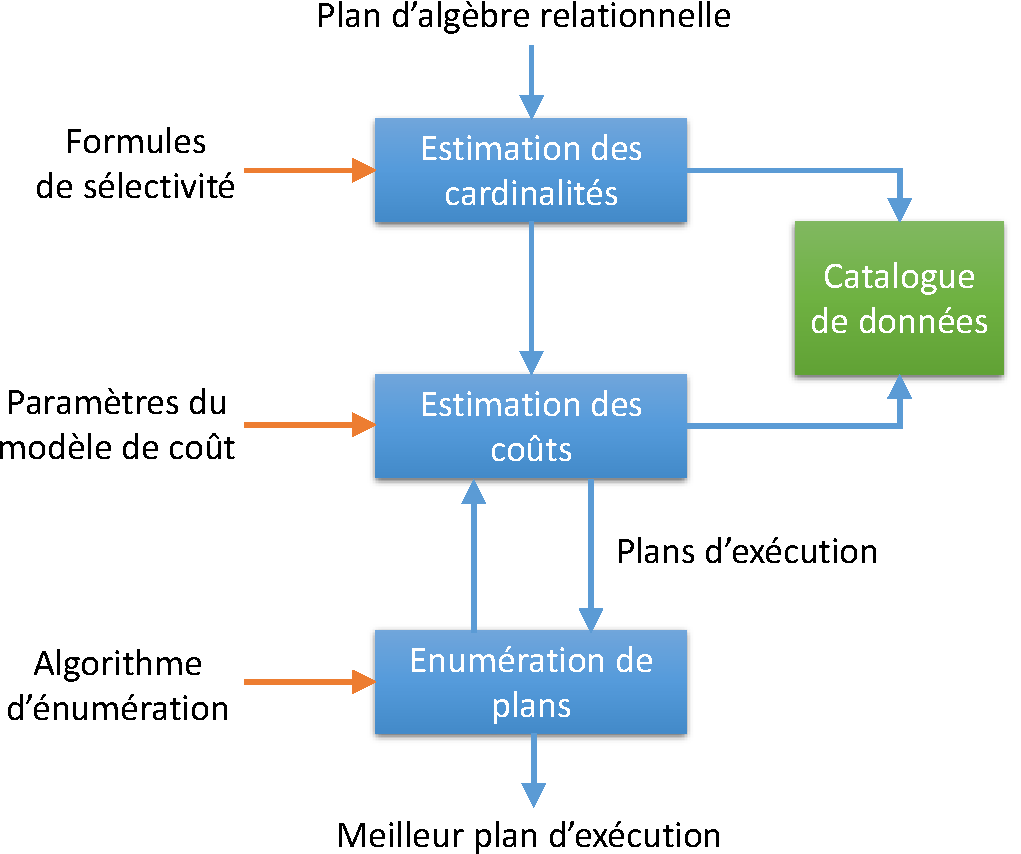
\includegraphics[scale=0.55]{chapitre2/chap2Fig/query-optimization.pdf}
\caption{Une architecture globale pour l'étape d'optimisation de requêtes.}
 \label{fig:query-optimization}
\end{center}
\end{figure}

En balayant entièrement la relation $R$, il est facile de compter le nombre de tuples $T(R)$ et aussi de découvrir le nombre de valeurs $V(R, a)$ différentes pour chaque attribut $a$. De plus, un SGBD peut calculer un \textit{histogramme} de distribution des valeurs d'un attribut donné. Si $V(R, A)$ n'est pas trop grand, l'histogramme peut être constitué du nombre (ou fraction) des tuples ayant chacune des valeurs de l'attribut $a$. Les histogrammes les plus courants sont \cite{Poosala96} :
\begin{itemize}
 \item \textbf{Largeur égale.} Divise l'intervalle de valeurs en intervalles de taille égale. On choisit une largeur $w$, avec une constante $v_0$. On fournit des comptages du nombre de tuples avec des valeurs $v$ dans les intervalles $v_0 \leq v < v_0 + w$, $v_0 + w \leq v < v_0 + 2 w$, etc. La valeur $v_0$ peut être la valeur la plus petite ou une borne inférieure sur les valeurs vues jusqu'ici.
 \item \textbf{Hauteur égale.} Ajuste les limites des intervalles de sorte que chaque intervalle ait le même nombre de valeurs. Ce sont les << centile\footnote{Un centile est chacune des 99 valeurs qui divisent les données triées en 100 parts égales, de sorte que chaque partie représente 1/100 de l'échantillon de population.} >> courants. On choisit une fraction $p$, et on énumère la valeur la plus petite, la valeur qui est la fraction $p$ du plus bas, la fraction $2p$ du plus bas, et ainsi de suite, jusqu'à la valeur la plus grande.
 \item \textbf{Valeurs les plus fréquentes.} Nous pouvons énumérer les valeurs les plus communes et leur nombre d'occurrences.
\end{itemize}

Les SGBD modernes comme IBM DB2, Informix, Microsoft SQL Server, Oracle et Sybase ASE utilisent la technique d'histogramme pour générer les statistiques sur les données \cite{Ramakrishnan03}.

\begin{figure}
  \centering
  \subfloat[Histogramme hauteur égale.\label{fig:histo-equidepth}]{
    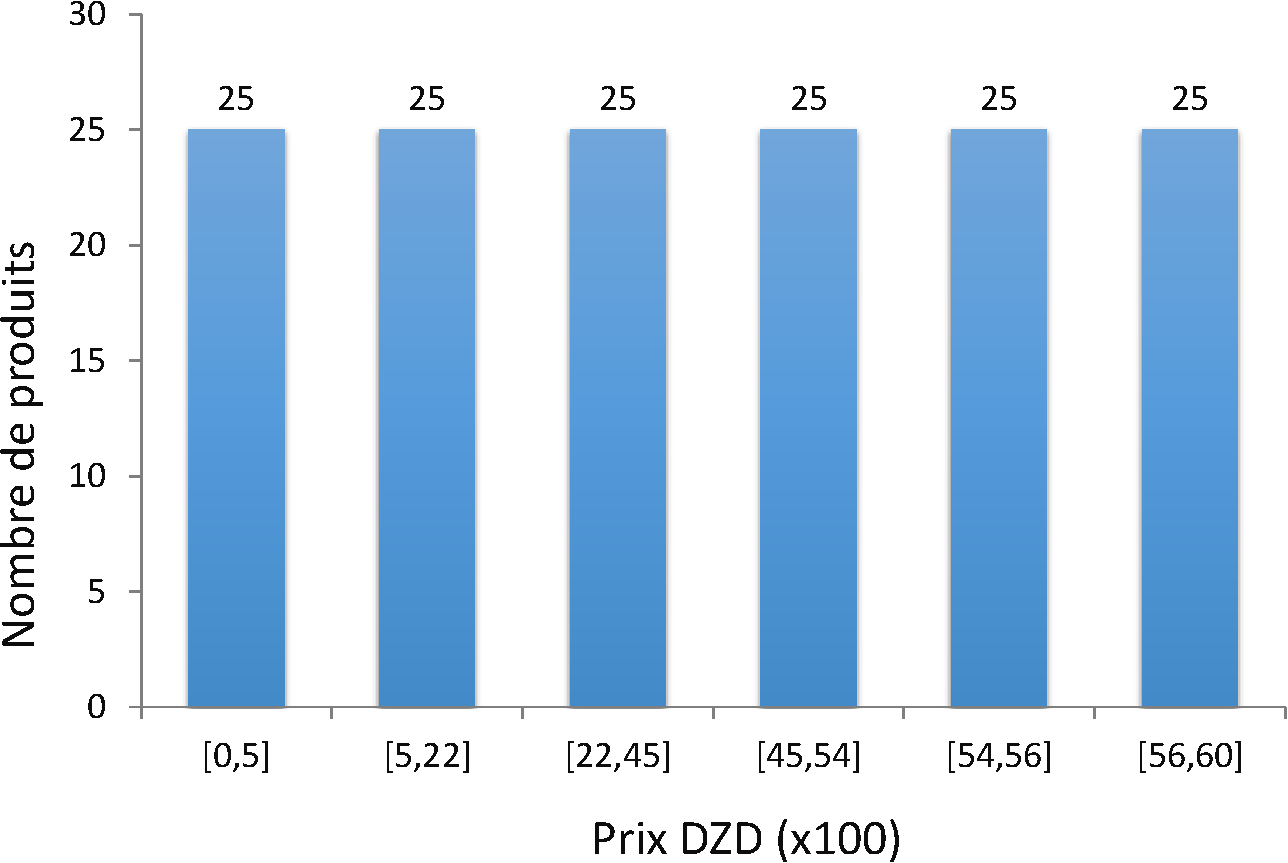
\includegraphics[scale=0.33]{chapitre2/chap2Fig/histo-equidepth.pdf}
  }
  \quad
  \subfloat[Histogramme largeur égale.\label{fig:histo-equiwidth}]{
    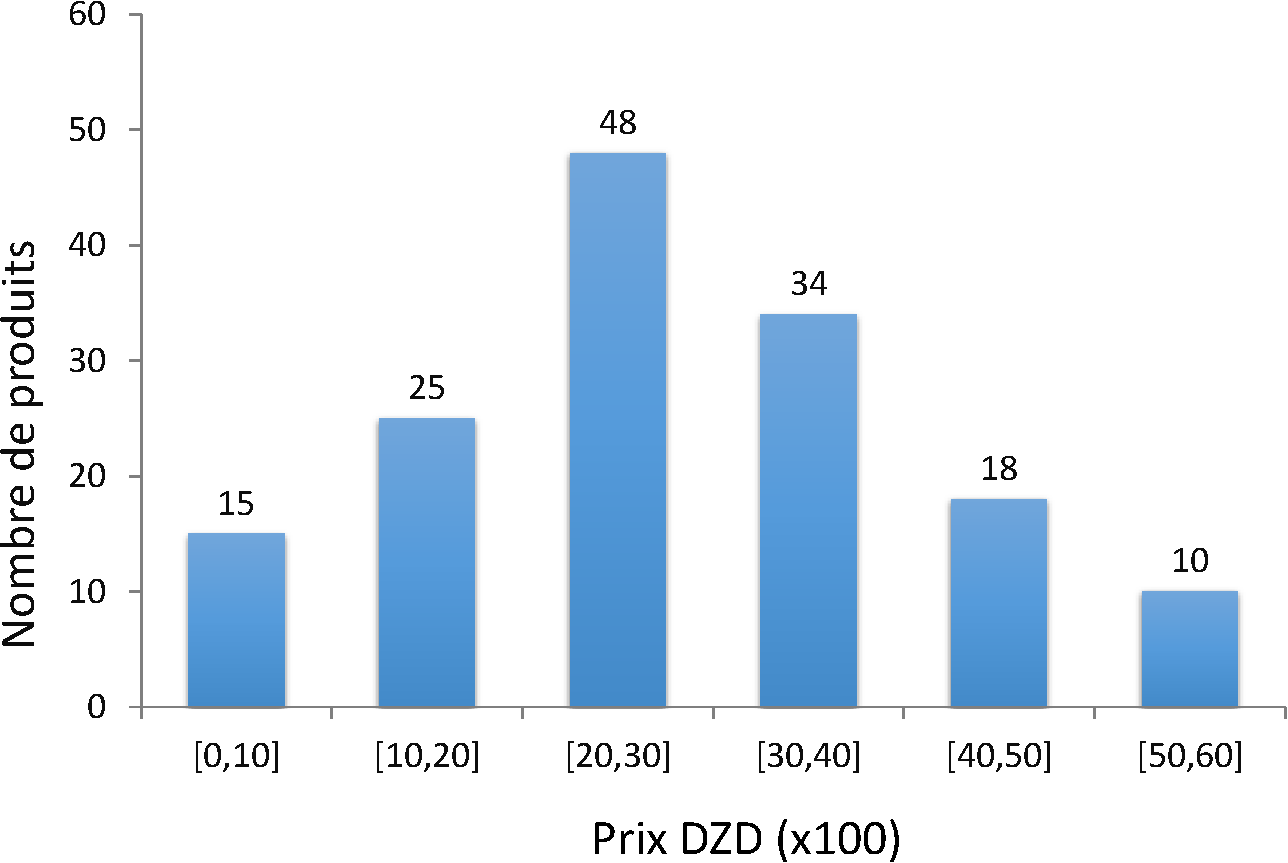
\includegraphics[scale=0.33]{chapitre2/chap2Fig/histo-equiwidth.pdf}
  }
  \caption{Exemples des histogrammes de distribution des valeurs d'attribut \textit{Prix} de la table \textit{Produit}.}\label{fig:histo-types}
\end{figure}

%\paragraph{Estimation de la taille des résultats intermédiaires}

\paragraph{Statistiques de système}\label{sec:costModelPram}
Le coût de l'évaluation des requêtes peut être mesuré en fonction d'un certain nombre de ressources système différentes. Les ressources ou paramètres les plus importants sont les suivants :

\begin{itemize}
 \item \textbf{Coût d'accès au stockage secondaire.} C'est le coût du transfert (lecture et écriture) des blocs de données entre le stockage de disque secondaire et les tampons de mémoire principale. Cela est également connu sous le nom de coût d'E/S (entrée/sortie) ou $\mathcal{C_{E/S}}$. Le coût de la recherche d'enregistrements dans un fichier disque dépend du type de structures d'accès sur ce fichier et la nature d'allocation des blocs de fichiers.
 \item \textbf{Coût de stockage sur disque.} C'est le coût de stockage sur disque de tous les fichiers intermédiaires générés par une stratégie d'exécution de la requête.
 \item \textbf{Coût de calcul.} C'est le coût d'exécution des opérations sur les enregistrements en mémoire tampon pendant l'exécution de la requête. Ces opérations comprennent la recherche, le tri, la fusion d'enregistrements pour une opération de jointure ou de tri et l'exécution de calculs sur les valeurs. Cela est également connu comme le coût de CPU (unité centrale de traitement) ou $\mathcal{C_{CPU}}$.
 \item \textbf{Coût d'utilisation de la mémoire.} C'est le coût correspondant au nombre de tampons mémoire nécessaires pendant l'exécution de la requête.
 \item \textbf{Coût de la communication.} Il s'agit du coût d'expédition de la requête et de ses résultats à partir du site de base de données vers le site ou le terminal d'où provient la requête. Dans les bases de données distribuées, il inclut également le coût du transfert des tables et des résultats entre différents ordinateurs au cours de l'évaluation des requêtes. Le coût de communication est abrégé $\mathcal{C_{COM}}$.
\end{itemize}

\subparagraph{Obtention des paramètres et leurs relations}
Les paramètres du modèle de coût, tels que le coût d'E/S et de CPU, doivent être calculés. Trois méthodes existent dans la littérature pour obtenir ces paramètres : \textit{analytique}, \textit{empirique} et \textit{dynamique} \cite{Ozsu11}.

\begin{enumerate}
 \item \textbf{Méthode analytique.} C'est l'approche classique employée par les premiers travaux sur les modèles de coût. Elle utilise des connaissances \textit{détaillées} sur le SGBD, l'implémentation des opérateurs algébriques, ainsi que les caractéristiques externes du matériel, pour déterminer analytiquement les informations sur les coûts \cite{Selinger79,Graefe93,Haas97}. Cette approche est adaptée par le SGBD open-source PostgreSQL \cite{Wu13b}.
 \item \textbf{Méthode empirique.} Cette approche traite le SGBD comme une \textit{boîte noire}. Elle consiste à identifier d'abord un ensemble de caractéristiques de requête et de données qui déterminent potentiellement les coûts des opérateurs. Puis, exécuter ces requêtes d'apprentissages sur le système. Ensuite, appliquer des modèles \textit{statistiques} ou \textit{d'apprentissage automatique} aux données collectées, et à partir de ceux-ci déterminer les paramètres finaux du modèle de coût et la relation entre eux \cite{Wu13,Ganapathi09,Li12a}. Cette approche est également utilisée par les SGBD commerciaux comme Oracle \cite{Chakkappen08}.
 \item \textbf{Méthode dynamique.} Les méthodes précédentes supposent que l'environnement d'exécution est toujours stable. Cependant, dans la plupart des cas, les facteurs d'environnement d'exécution changent fréquemment, tels que la charge et la vitesse du CPU, le débit d'E/S, la disponibilité de mémoire, le schéma et les données de la BD, etc. Cette troisième approche se base sur la méthode empirique, et de plus, elle surveille le comportement d'exécution du SGBD et collecte et ajuste dynamiquement les informations sur les coûts pour faire face au changement d'environnement \cite{Duan09,Sheikh11,Khattab13}.
\end{enumerate}

% TODO: 
% Weighted sum of costs
% C_Q = $\mathcal{C_{e/s}$ + $\mathcal{C_{cpu}$ + $\mathcal{C_{com}$

%\paragraph{Modèles de coût des opérateurs}
Compte tenu d'un plan d'exécution, nous pouvons maintenant estimer son coût en utilisant l'estimation de la cardinalité des résultats intermédiaires faite par les techniques de \ref{sec:cardinalityEstimation} de l'\ref{annex:CostModelEstimations}, couplées aux estimations de coûts pour divers algorithmes et méthodes d'accès décrits au \ref{sec:operatorsCostModel} de l'\ref{annex:CostModelEstimations}.

\paragraph{Approches pour l'énumération des plans physiques} % 16.5.4 Approaches to Enum erating Physical Plans (db complete book)
Maintenant, considérons l'utilisation des estimations de coûts dans la conversion d'un plan de requête logique en un plan de requête physique. L'approche de référence, appelée \textit{exhaustive}, consiste à considérer toutes les combinaisons de choix possible. Chaque plan physique est affecté à un coût estimé, et celui avec le plus petit coût est sélectionné \cite{Elmasri08}. Cependant, il existe d'autres approches pour sélectionner un plan physique. En terme d'exploration de l'espace des plans physiques possibles, il existe deux approches principales : (1) \textit{descendante} et (2) \textit{ascendante}. Dans la première approche, l'estimation se fait à partir de la racine de l'arbre du plan de requête logique vers le bas en choisissant le meilleur choix à chaque étape. Cette approche est adoptée par Volcano, Cascades, Tandem et Microsoft SQL Server \cite{Lohman07}. Tandis que dans la deuxième approche, l'estimation se fait à partir des feuilles vers la racine. Cette approche est utilisée dans System R, DB2, Oracle et Informix \cite{Lohman07}. Nous décrirons ensuite les différentes techniques proposées dans la littérature pour l'énumération des plans physiques \cite{GarciaMolina08, Elmasri08}.

\begin{itemize}
 \item \textbf{Sélection heuristique.} Une option est d'utiliser la même approche pour sélectionner un plan physique qui est généralement utilisé pour sélectionner un plan logique : faire une séquence de choix basée sur l'heuristique (\ref{sec:transformation}). Il existe d'autres heuristiques qui peuvent être appliquées. Par exemple, si le plan logique appelle une sélection $\sigma_{A=c}(R)$, et la relation stockée $R$ a un index sur l'attribut $A$, effectuer un balayage d'index pour obtenir seulement les tuples de $R$ avec une valeur de $A$ égale à $c$.
 \item \textbf{Séparation et évaluation (\textit{Branch-and-Bound}).} Cette approche, souvent utilisée en pratique, commence par utiliser des heuristiques pour trouver un bon plan physique pour l'ensemble du plan de requête logique. Soit $\mathcal{C}$ le coût de ce plan. Alors, lorsque nous considérons d'autres plans pour les sous-requêtes, nous pouvons éliminer tout plan qui a un coût supérieur à $\mathcal{C}$, puisque ce plan ne pourrait pas participer à un plan complet meilleur que celui que nous avons déjà. De même, si nous trouvons un plan qui a un coût moins que $\mathcal{C}$, nous remplaçons $\mathcal{C}$ par le coût de ce meilleur plan dans l'exploration ultérieure de l'espace des plans de requêtes physiques.
 \item \textbf{Escalade (\textit{Hill climbing}).} Cette approche, dans laquelle nous cherchons une << vallée >> dans l'espace des plans physiques et de leurs coûts, commence avec un plan physique heuristiquement choisi. Nous pouvons alors apporter de petits changements au plan, par exemple en remplaçant une méthode pour exécuter un opérateur par une autre, ou en réordonnant des jointures en utilisant les lois associatives et/ou commutatives, pour trouver des plans << proches >> qui ont un coût inférieur. Lorsque nous trouvons un plan tel qu'aucune modification ne permet pas de donner un plan de coût inférieur, nous choisissons ce plan comme un plan physique.
 \item \textbf{Programmation dynamique.} Dans cette variante de la stratégie ascendante, nous gardons pour chaque sous-expression seulement le plan de moindre coût. Au fur et à mesure que nous traversons l'arbre, nous considérons les implémentations possibles de chaque nœud, en supposant que le meilleur plan pour chaque sous-expression est également utilisé.
 \item \textbf{System-R.} Cette approche améliore l'approche de programmation dynamique en gardant pour chaque sous-expression non seulement le plan de moindre coût, mais certains autres plans qui ont un coût plus élevé, alors qu'ils produisent un résultat trié dans un ordre qui peut être utile plus haut dans l'expression de l'arbre. Car les attributs déjà triés dans une opération tel que la sélection, le groupement ou la jointure peuvent être utilisés dans un algorithme de tri d'une manière efficace \cite{Selinger79}.
\end{itemize}

\begin{figure}
  \centering
  %\small
  \subfloat[Arbre de jointure linéaire gauche.\label{fig:left-deep-join-tree}]{
    {\tikzset{>=latex}

\begin{forest} for tree={align=center}
[$\bowtie$
    [$\bowtie$
		[$\bowtie$
			[$R$]
			[$S$]
		]
		[$T$]
    ]
    [$U$]
]
\end{forest}
}
  }
  \quad
  \subfloat[Arbre de jointure ramifié.\label{fig:bushy-join-tree}]{
    {\begin{forest} for tree={align=center}
[$\bowtie$
	[$\bowtie$
		[$R$]
		[$S$]
	]
    [$\bowtie$
		[$T$]
		[$U$]
    ]
]
\end{forest}
}
  }
  \quad
  \subfloat[Arbre de jointure linéaire droit.\label{fig:right-deep-join-tree}]{
    {\begin{forest} for tree={align=center}
[$\bowtie$
	[$R$]
    [$\bowtie$
		[$S$]
		[$\bowtie$
			[$T$]
			[$U$]
		]
    ]
]
\end{forest}
}
  }
  \caption{Exemple des méthodes pour la jointure de quatre relations.}\label{fig:join-tree-examples}
\end{figure}

\subparagraph{Problème d'ordre de jointure} % 19.5.3 Multirelation Queries and JOIN Ordering Choices
Les règles de transformation algébriques pour l'opération de jointure peuvent produire de nombreuses expressions de jointure équivalentes. En conséquence, le nombre d'arborescences de requêtes alternatives croît très rapidement avec l'augmentation du nombre de jointures dans une requête. En général, pour un bloc de requête comportant $n$ relations, il existe $n!$ ordres de jointure \cite{Elmasri08}.
Un arbre d'une requête ayant plus de deux jointures peut être exprimé en trois structures : 
\begin{enumerate}
 \item \textbf{Arbre de jointure linéaire gauche.} Est un arbre binaire où l'enfant gauche de chaque nœud de feuille est une relation de base (\ref{fig:left-deep-join-tree}).
 \item \textbf{Arbre de jointure linéaire droit.} Est un arbre binaire dans lequel l'enfant droit de chaque nœud non-feuille est toujours une relation de base. Un exemple est illustré dans la \ref{fig:right-deep-join-tree}.
 \item \textbf{Arbre de jointure ramifié.} Est un arbre binaire où l'enfant gauche ou droit d'un nœud interne peut être un nœud de jointure (\ref{fig:bushy-join-tree}). 
\end{enumerate}

La plupart des optimiseurs de requêtes considèrent les arbres de jointure linéaire gauche comme arbre de jointure préféré, puis choisi un parmi les $n!$ ordres de jointure possibles. Le problème d'ordre de jointure peut être résolu par trois classes d'algorithme : déterministe, aléatoire ou génétique (pour plus de détails, voir l'étude de \cite{Vellev09}).

\begin{itemize}
 \item \textbf{Algorithmes déterministes.} Également connu sous le nom d'algorithme de programmation dynamique de recherche exhaustive. Les algorithmes de cette classe effectuent une certaine recherche déterministe de l'espace de solution, soit par traverse complète, soit par l'application de certaines heuristiques d'élagage de l'espace \cite{Selinger79,Steinbrunn97}.
 \item \textbf{Algorithmes aléatoires.} Ces algorithmes effectuent une marche aléatoire dans l'espace de la solution, se déplaçant d'un point à un autre. Un déplacement est possible si la solution du premier point peut être transformée en solution du second point en lui appliquant une seule règle de transformation. L'exécution de l'algorithme se termine soit quand aucun déplacement valide ne peut être effectué ou quand un temps d'exécution prédéfini s'est écoulé. La meilleure solution trouvée pendant la marche aléatoire est le résultat de l'optimisation \cite{Ioannidis87,Ioannidis90}.
 \item \textbf{Algorithmes génétiques.} Les algorithmes génétiques imitent l'évolution biologique pour rechercher la solution optimale. L'idée principale est, à partir d'un ensemble initial (population) de solutions, génère des descendants par des opérations de croisement aléatoire et mutation. Les meilleurs individus de la population survivent à chaque génération et forment la nouvelle population. L'algorithme s'arrête soit après un certain nombre de générations, soit lorsque la population devient homogène au-dessus d'un certain seuil suivant de la fonction de coût \cite{Bennett91,Stillger96}.
\end{itemize}

\subsubsection{Exécution}
La dernière étape du processus est l'exécution de la requête. Dans cette étape, toutes les opérations d'E/S et de CPU indiquées dans le plan physique sont exécutées.
Un opérateur physique d'une requête peut être exécuté en mode \textit{matérialisé} ou \textit{pipeline} et/ou \textit{parallèle}.

\paragraph{Matérialisée}
Avec une exécution matérialisée, le résultat d'une opération est stocké comme une relation temporaire. Chaque résultat est physiquement matérialisé sur le dispositif de stockage et s'ajoute au coût global du traitement des requêtes. Par exemple, le résultat de l'opération $\bowtie$ peut être calculée et stocké comme une relation temporaire. Ce résultat est considéré comme entrée par l'algorithme qui calcule l'opération $\pi$ pour produire le résultat final de la requête. La génération et le stockage de gros fichiers temporaires sur le disque prend beaucoup de temps et peuvent être inutile dans de nombreux cas, car ces fichiers seront immédiatement utilisés comme entrée pour la prochaine opération \cite{Elmasri08}.

\paragraph{Pipeline}
D'autre part, avec l'exécution en pipeline, lorsque les tuples résultants d'une opération sont produits, ils sont envoyés directement à l'opération suivante dans la séquence de requête. Par exemple, les tuples sélectionnés d'une relation sont produits par l'opération $\sigma$, et placés dans un tampon mémoire. L'opération $\bowtie$ consomme alors les tuples de la mémoire tampon, et les tuples qui résultent sont pipelinés à l'opération $\pi$. L'avantage du pipelining est les économies de coût d'écriture des résultats intermédiaires sur le disque et la relecture pour l'opération suivante. Il permet également de produire des résultats rapidement avec certaines opérations algébriques.

\begin{figure}
\begin{center}
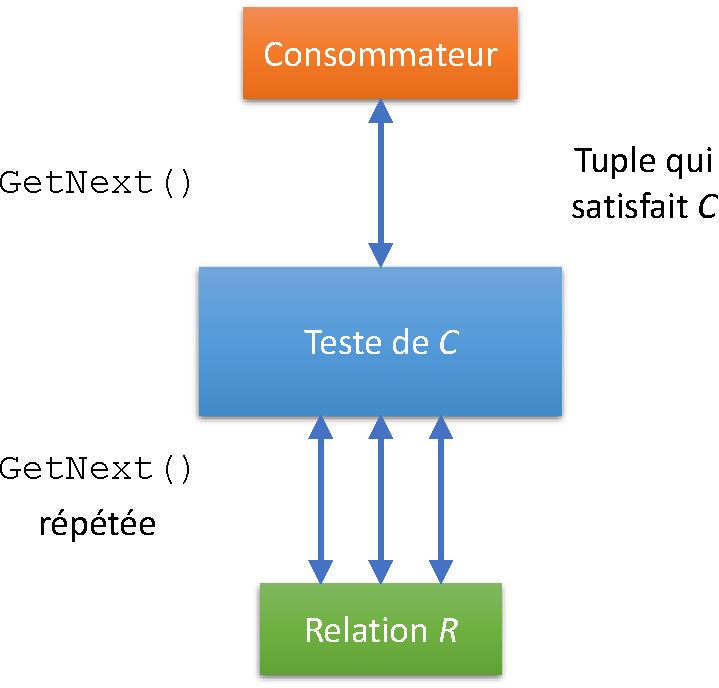
\includegraphics[scale=0.55]{chapitre2/chap2Fig/pipeline-example.pdf}
\caption{Exécution d'une sélection en mode pipeline à l'aide d'itérateurs.}
 \label{fig:pipeline-example}
\end{center}
\end{figure}

Différents algorithmes pour des opérations algébriques impliquent la lecture d'un ou plusieurs fichiers comme entrée, le traité, et ensuite la génération d'un fichier de résultat comme sortie. Si l'opération est mise en œuvre de telle sorte qu'elle produit qu'un tuple à la fois, elle peut être considérée comme un \textit{itérateur}. Par exemple, une implémentation pour la jointure à boucle imbriquée génère un tuple à la fois comme sortie après chaque jointure. L'interface itérateur comprend généralement les méthodes suivantes \cite{chaudhuri04} :

\begin{enumerate}
 \item \textbf{\texttt{Open()}} : Cette méthode initialise l'opérateur en allouant des tampons pour son entrée et sa sortie et en initialisant toutes les structures de données nécessaires à l'opérateur. Il est également utilisé pour transmettre des arguments tels que les conditions de sélection nécessaires pour effectuer l'opération. Il appelle à son tour \texttt{Open()} pour obtenir les arguments dont il a besoin.
 \item \textbf{\texttt{GetNext()}} : Cette méthode appelle le \texttt{GetNext()} sur chacun de ses arguments d'entrée et appelle le code spécifique à l'opération exécutée sur les entrées. Le prochain tuple de sortie généré est renvoyé, et l'état de l'itérateur est mis à jour suivant la quantité d'entrée traitée. Lorsque aucun tuple ne peut être renvoyé, il place une valeur spéciale dans le tampon de sortie.
 \item \textbf{\texttt{Close()}} : Cette méthode met fin à l'itération après la génération de tous les tuples possible ou si le nombre requis/demandé de tuples a été retourné. Elle appelle également \texttt{Close()} sur les arguments de l'itérateur.
\end{enumerate}

Cependant, certains opérateurs physiques ne supportent pas le concept d'interface itérateur et ne peuvent donc pas prendre en charge le pipeline. Comme par exemple l'opérateur de tri et de groupement, car ils ne produisent aucune sortie tant qu'ils n'ont pas consommé leurs entrées complètement \cite{luo04}.

\begin{example}
 Le consommateur du résultat du pipeline appelle \texttt{GetNext()} chaque fois qu'un tuple est nécessaire. Dans le cas d'une projection, il suffit d'appeler \texttt{GetNext()} une fois sur la source des tuples, ensuite projeter ce tuple de manière appropriée et retourner le résultat au consommateur. Pour une sélection $\sigma_c$, il peut être nécessaire d'appeler \texttt{GetNext()} plusieurs fois à la source, jusqu'à ce qu'un tuple qui satisfait la condition $C$ est trouvé. La \ref{fig:pipeline-example} illustre ce processus.
\end{example}

\paragraph{Parallèle}
Les opérations de base de données, qui prennent souvent beaucoup de temps et impliquent beaucoup de données, peuvent généralement bénéficier d'un traitement parallèle. Trois approches principales ont été proposées pour les bases de données parallèles. Ils correspondent à trois configurations matérielles différentes de processeurs et de périphériques de stockage secondaires (disques) pour supporter le parallélisme. Dans une \textit{architecture à mémoire partagée}, plusieurs processeurs sont connectés à un réseau d'interconnexion et peuvent accéder à une région de mémoire principale commune. Le deuxième type d'architecture est connu sous le nom \textit{d'architecture à disque partagé}. Dans cette architecture, chaque processeur a sa propre mémoire, qui n'est pas accessible à partir d'autres processeurs. Cependant, chaque machine a accès à tous les disques à travers le réseau d'interconnexion. Le troisième type est \textit{l'architecture sans partage}. Dans cette architecture, chaque processeur accède à sa propre mémoire principale et à son stockage disque \cite{Taniar08}.

L'architecture sans partage offre la possibilité d'atteindre le parallélisme dans le traitement des requêtes à quatre niveaux, y compris (1) le parallélisme inter-requêtes, (2) le parallélisme intra-requêtes, (3) le parallélisme inter-opérations et (4) le parallélisme intra-opérations \cite{Ozsu11}.

\begin{enumerate}
 \item \textbf{Parallélisme inter-requêtes.} Le parallélisme inter-requêtes est le << parallélisme entre les requêtes >>, c'est-à-dire que des requêtes ou des transactions différentes sont exécutées en parallèle les unes avec les autres d'une façon concurrente. L'utilisation principale du parallélisme entre les requêtes consiste à mettre à l'échelle les systèmes de traitement des transactions pour supporter un grand nombre de transactions par seconde.
 \item \textbf{Parallélisme intra-requêtes.} Une requête est divisée en plusieurs opérations. Le parallélisme intra-requête est une exécution d'une seule requête en parallèle sur plusieurs processeurs et disques. Dans ce cas, les opérations multiples dans une requête sont exécutées en parallèle. Par conséquent, le parallélisme intra-requête est le << parallélisme au sein d'une requête >>.
 \item \textbf{Parallélisme inter-opérations.} Puisque les opérations de base de données fonctionnent sur des tables contenant de grands ensembles de données, nous pouvons paralléliser les opérations en les exécutant en parallèle sur différents sous-ensembles de la table. Par conséquent, le parallélisme inter-opérations est souvent appelé parallélisme partitionné, c'est-à-dire parallélisme dû à la partition des données. Comme le nombre d'enregistrements dans une table peut être important, le degré de parallélisme est potentiellement énorme. Par conséquent, le parallélisme inter-opérations est naturel dans les systèmes de base de données.
 \item \textbf{Parallélisme intra-opérations.} Le parallélisme intra-opérations est là où le parallélisme est créé en exécutant simultanément différentes opérations au sein d'une même requête. Par exemple, la séquence d'opérations $R \bowtie S \bowtie T \bowtie U$. Dans ce cas, on peut traiter le $R \bowtie S$ en parallèle avec le $T \bowtie U$.
\end{enumerate}

% TODO: Vers l'intégration de l'énergie dans la phase de traitement de requêtes
\subsubsection{Bilan et discussion}
Comme nous avons vu au cours de cette section, le principal objectif lors du traitement de requête par un SGBD est la minimisation du temps de réponse des requêtes, à l'aide de techniques sophistiquées, qui comprennent des algorithmes pour sélectionner et exécuter un plan optimal pour une requête. Cependant, nous proposons une nouvelle façon de penser sur le traitement et l'optimisation des requêtes. L'idée est de reformuler le problème d'optimisation des requêtes en : \textit{trouvant et exécutant le plan le plus éco-énergétique qui répond à un certain objectif de temps de réponse}. Cela peut être achevé (1) en étendant l'optimiseur de requêtes existant avec un modèle de coût de consommation d'énergie, en plus du modèle de temps de réponse traditionnel, et (2) avec un modèle d'évaluation des coûts des plans d'exécution. Le modèle d'évaluation des coûts est utilisé pour sélectionner les plans d'exécution avec la capacité d'ajuster dynamiquement sa préférence entre l'énergie et la performance dans la sélection du plan de requête.

\section{Compromis entre la performance et l'énergie : Optimisation multi-objectifs}
La proposition des techniques, comme les vues matérialisées ou le traitement de requêtes, pour minimiser l'énergie dans les base de données est une seule partie du problème, car ces techniques ne garantissent pas un temps de réponse acceptable des traitements du SGBD. La deuxième partie du problème consiste à développer des techniques qui offrent le meilleur compromis entre la minimisation du temps de réponse aux requêtes et la minimisation de la consommation d'énergie du système. Ceci est considéré comme un problème \textit{multi-objectif} parce que le problème consiste à optimiser plus d'un problème simultanément.
Alors que dans l'optimisation mono-objectif la solution optimale est généralement clairement définie, cela n'est pas valable pour les problèmes d'optimisation multi-objectifs. Au lieu d'un seul optimum, il existe plutôt un ensemble de compromis alternatives, généralement connues sous le nom de solutions \textit{Pareto-optimales}. Ces solutions sont optimales dans le sens qu'aucune autre solution dans l'espace de recherche est meilleure lorsque tous les objectifs sont pris en compte.
Dans cette section, les principes de l'optimisation multi-objectifs sont décrits et les concepts de base sont formellement définis. Ceci est suivi d'une discussion sur les approches classiques et les algorithmes évolutionnaires utilisés pour approcher l'ensemble des solutions Pareto-optimales. Ensuite, nous exposons l'état de l'art sur l'optimisation multi-objectifs dans le contexte des bases de données, et plus particulièrement, le problème de sélection de vues matérialisées et le traitement de requêtes.

\subsection{Problème d'optimisation multi-objectifs}
Généralement, un problème d'optimisation multi-objectifs ($\mathcal{\acrshort[hyper=false]{PMO}}$) comprend un ensemble de $n$ paramètres (variables de décision), un ensemble de $k$ fonctions objectifs et un ensemble de $m$ contraintes. L'objectif d'optimisation est de minimiser ou maximiser les $k$ fonctions objectifs en respectant les contraintes $m$. Plus formellement, le $\mathcal{PMO}$ est défini comme suit \cite{Zhou2011} :
\begin{alignat}{2}
& \text{minimiser} \quad && y = f(x) = (f_1(x), f_2(x), \cdots, f_k (x)) \nonumber \\
& \text{avec}      \quad && e(x) = (e_1(x), e_2(x), \cdots, e_m(x)) \leq 0 \nonumber\\
& \text{et}        \quad && x = (x_1, x_2, \cdots , x_n ) \in X \nonumber \\
&                  \quad && y = (y_1, y_2, \cdots , y_k ) \in Y
\end{alignat}
Où $x$ est le vecteur de décision, $y$ est le vecteur objectif, $X$ est désigné comme l'espace de décision, et $Y$ est appelé l'espace objectif. Les contraintes $e(x) \leqslant 0$ déterminent l'ensemble des \textit{solutions réalisables}. L'ensemble des solutions réalisable $X_f$ est défini comme l'ensemble des vecteurs de décision $x$ qui satisfont les contraintes $e(x)$ :
\begin{equation}
 X_f = \{x \in X | e(x) \leqslant 0\}
\end{equation} 
L'image de $X_f$, c'est-à-dire la région réalisable dans l'espace objectif, est désignée par :
\begin{equation}
 Y_f = f(X_f) = \bigcup_{x \in X_f} \{f(x)\}
\end{equation} 
Dans le reste de la section, nous supposons un problème de minimisation. Pour les problèmes de maximisation ou de maximisation/minimisation mixtes, les définitions présentées ici sont similaires.

\begin{figure}
  \centering
  \subfloat[Exemple de front d'optimum de Pareto.\label{fig:pareto-optimality}]{
    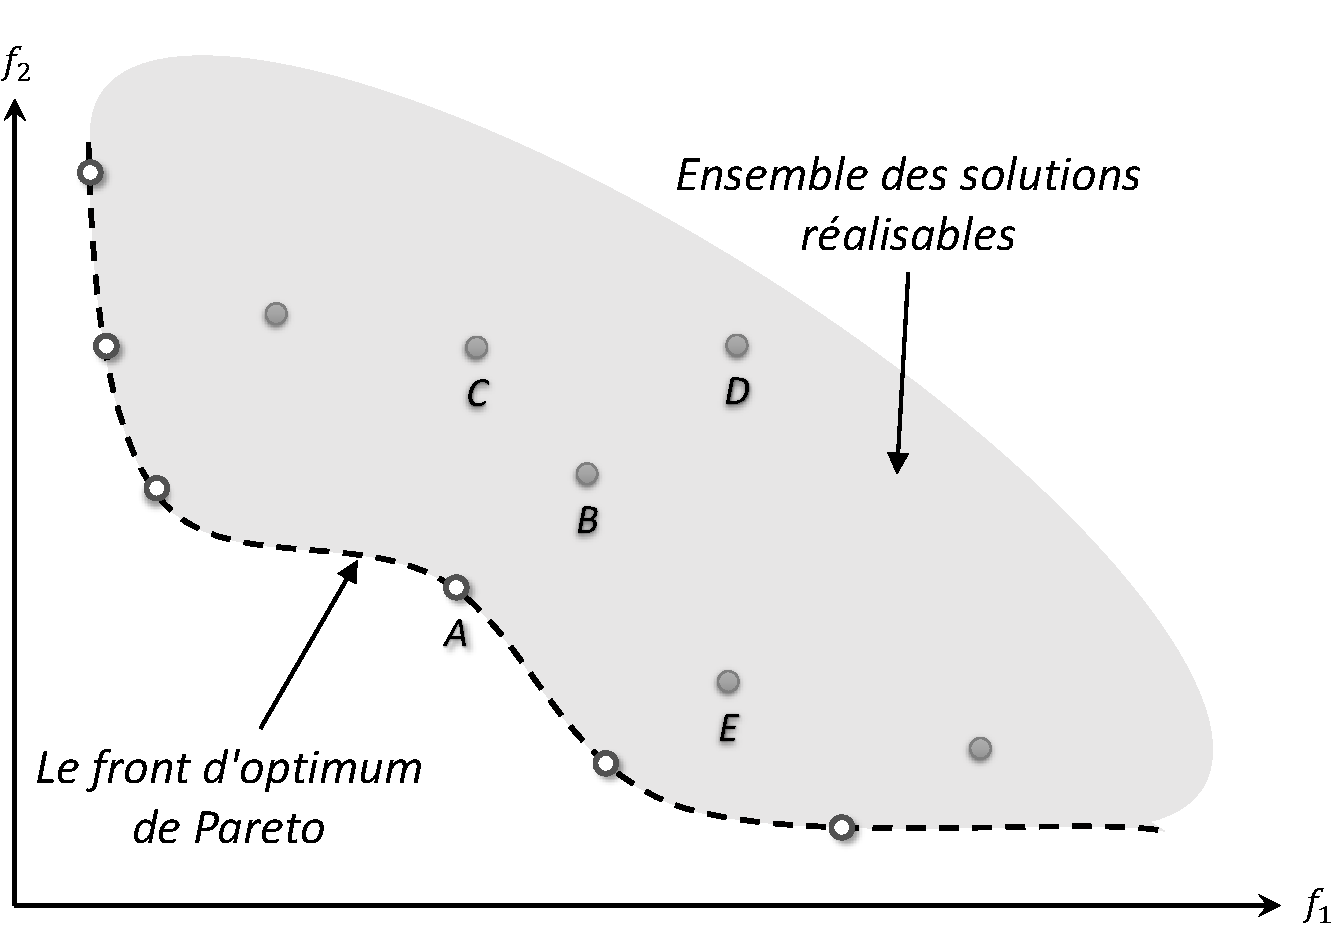
\includegraphics[scale=0.33]{chapitre2/chap2Fig/pareto-optimality.pdf}
  }
  \quad
  \subfloat[Exemple des relations entre les solutions.\label{fig:pareto-solutions}]{
    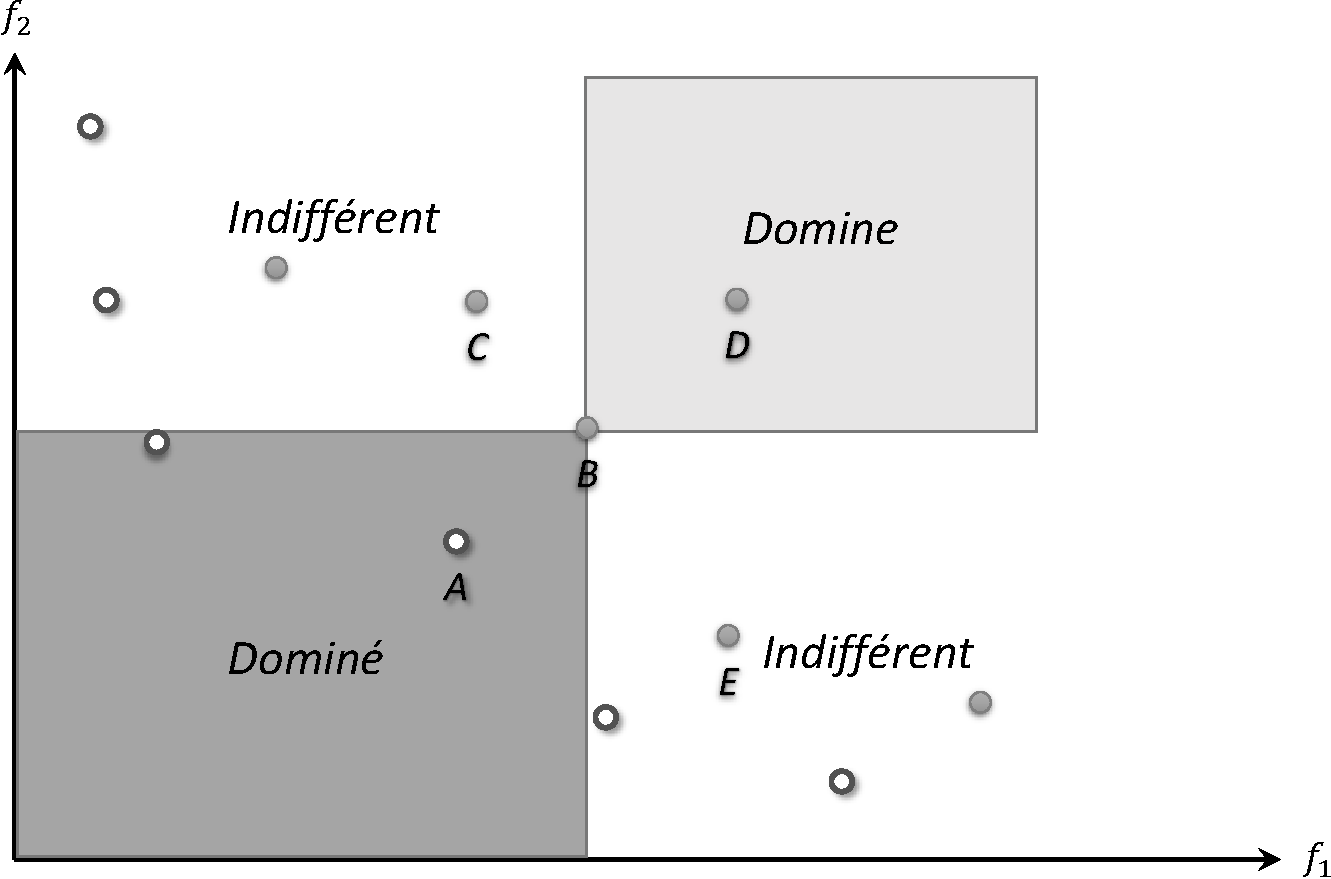
\includegraphics[scale=0.33]{chapitre2/chap2Fig/pareto-solutions.pdf}
  }
  \caption{Exemples de la notion de dominance de Pareto dans l'espace objectif.}\label{fig:pareto-optimality-example}
\end{figure}

Dans l'optimisation mono-objectif ($\mathcal{\acrshort[hyper=false]{OMO}}$), l'ensemble réalisable est totalement ordonné selon la fonction objectif $f$ : pour deux solutions $a$, $b \in X_f$ soit $f(a) \leqslant f(b)$ ou $f(b) \leqslant f(a)$. Le but est de trouver la ou les solutions qui donnent la valeur minimale de $f$ \cite{Deb01}. Cependant, lorsque plusieurs objectifs sont impliqués, la situation change : $X_f$ en général n'est pas totalement ordonné, mais partiellement ordonné. Ceci est illustré à la \ref{fig:pareto-optimality}. La solution représentée par le point $B$ est meilleure que la solution représentée par le point $D$. Elle serait préférable si c'est un problème $\mathcal{OMO}$. En effet, dans le cas entre les points $C$ et $D$ : malgré que les $f_2$ sont égaux, $C$ obtient de meilleures valeurs dans $f_1$ que $D$. Pour exprimer mathématiquement cette situation, les relations $=$, $\leqslant$ et $<$ sont étendues aux vecteurs objectifs par analogie avec le cas $\mathcal{OMO}$. Pour deux vecteurs objectifs quelconques $u$ et $v$ :
\begin{alignat}{2}
& u = v         \quad && \Leftrightarrow \quad \forall i \in \{1,\cdots,k\} : u_i = v_i \nonumber \\
& u \leqslant v \quad && \Leftrightarrow \quad \forall i \in \{1,\cdots,k\} : u_i \leqslant v_i \nonumber \\
& u < v         \quad && \Leftrightarrow \quad u \leqslant v \wedge u \neq v 
\end{alignat}
En utilisant cette notion, on considère que $A < B$, $B < D$, et par conséquent, $A < D$. Cependant, en comparant $B$ et $E$ dans les deux fonctions objectives, aucune des solutions ne peut être considérée comme meilleure, puisque $B \nleqslant E$ et $E \nleqslant B$. Par conséquent, deux vecteurs de décision $a$, $b$ peuvent avoir trois possibilités avec $\mathcal{PMO}$ en ce qui concerne la relation $\leqslant$ (contrairement à deux possibilités avec $\mathcal{OMO}$) : $f(a) \leqslant f(b)$, $f(b) \leqslant f(a)$ ou $f(a) \nleqslant f(b) \wedge f(b) \nleqslant f(a)$. Les notions suivantes sont utilisées pour classer les différentes situations.
\begin{definition}
 (\textit{Dominance de Pareto}) Pour deux vecteurs de décision quelconques $a$ et $b$,
 \begin{alignat}{2}
  & a \prec b        \; \text{($a$ domine $b$)}          \quad && \Leftrightarrow \quad f(a) < f(b) \nonumber \\
  & a \preccurlyeq b \; \text{($a$ domine faiblement $b$)} \quad && \Leftrightarrow \quad f(a) \leqslant f(b) \nonumber \\
  & a \sim b         \; \text{($a$ est indifférent à $b$)} \quad && \Leftrightarrow \quad f(a) \nleqslant f(b) \wedge f(b) \nleqslant f(a) 
  \end{alignat}
\end{definition}

Dans la \ref{fig:pareto-solutions}, le rectangle gris clair encapsule la région dans l'espace objectif qui est \textit{dominée} par le vecteur de décision représenté par $B$. Le rectangle gris foncé contient les vecteurs objectifs dont les vecteurs de décision correspondant \textit{dominent} la solution associée à $B$. Toutes les solutions pour lesquelles le vecteur objectif résultant n'est dans aucun rectangle sont \textit{indifférentes} à la solution représentée par $B$.

Sur la base du concept de dominance de Pareto, le \textit{critère d'optimalité} pour les $\mathcal{PMO}$ peut être introduit. Toujours en référence à la \ref{fig:pareto-solutions}, $A$ est unique parmi $B$, $C$, $D$ et $E$ : son vecteur de décision $a$ correspondant n'est pas dominé par aucun autre vecteur de décision. Cela signifie que $a$ est optimal dans le sens où il ne peut pas être amélioré dans une objective sans causer une dégradation dans au moins une autre objective. Ces solutions sont appelées \textit{optimum de Pareto} \cite{Branke08}.

\begin{definition}
(\textit{Optimalité de Pareto}) On dit qu'un vecteur de décision $x \in X_f$ est non-dominé pour un ensemble $A \subseteq X_f$ si et seulement si :
\begin{equation}
\nexists \; a \in A: a \prec x
\end{equation} 
En outre, $x$ est dit \textit{optimum de Pareto} si et seulement si $x$ est non-dominé pour $X_f$.
\end{definition}
Dans la \ref{fig:pareto-solutions}, les points blancs représentent des solutions optimales de Pareto. Ils sont indifférents les uns aux autres. Cela rend la principale différence à la $\mathcal{OMO}$ clair : il n'existe pas de solution optimale unique, mais plutôt un ensemble de compromis optimaux. Aucune solution d'entre elles ne peut être identifiée comme meilleure que les autres à moins que l'information de préférence soit incluse (par exemple, un classement des objectifs).

L'ensemble de toutes les solutions optimales de Pareto est appelé \textit{ensemble d'optimum de Pareto}; Les vecteurs objectifs correspondants forment \textit{le front ou la surface d'optimum de Pareto} \cite{Deb01}.

\begin{figure}
\begin{center}
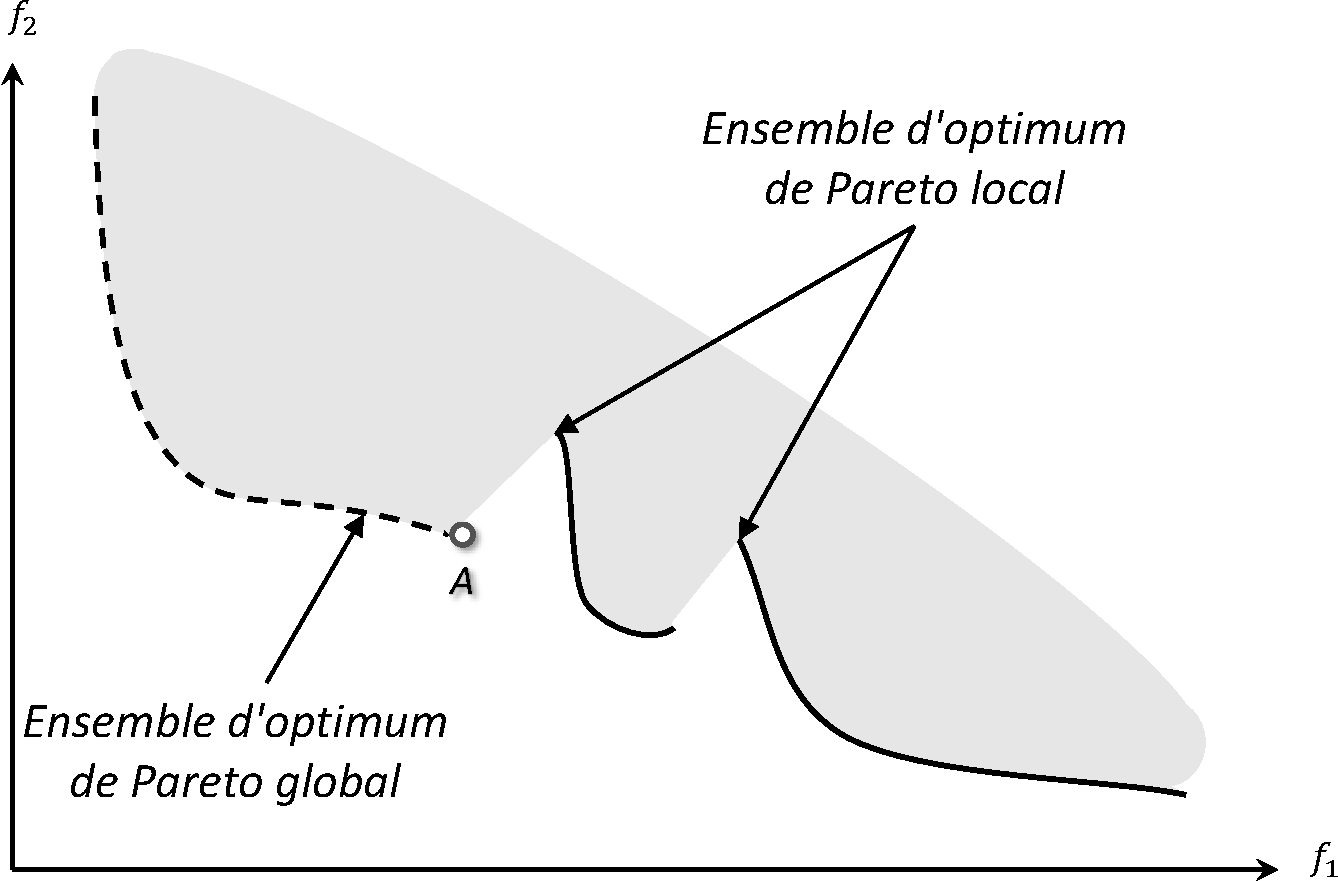
\includegraphics[scale=0.4]{chapitre2/chap2Fig/pareto-global-local.pdf}
\caption{Exemple d'ensembles de solutions localement optimales et de solutions globalement optimales dans l'espace objectif.}
 \label{fig:pareto-global-local}
\end{center}
\end{figure}

\begin{definition}
 (\textit{Ensembles et fronts non dominés}) Soit $A \subseteq X_f$. La fonction $p(A)$ donne l'ensemble des vecteurs de décision non dominés en $A$ :
 \begin{equation}
  P(A) = \{a \in A | a \text{ est non-dominé sur } A\}
 \end{equation}
 $p(A)$ est l'ensemble non-dominé sur $A$, l'ensemble correspondant de vecteurs objectifs $f(p(A))$ est le front non-dominé de $A$. En outre, $X_p = p(X_f)$ est nommé l'ensemble d'optimum de Pareto et $Y_p = f (X_p)$ est désigné comme le front d'optimum de Pareto.
\end{definition}

L'ensemble d'optimum de Pareto comprend les solutions globalement optimales. Cependant, il peut y avoir des optima locaux qui constituent un ensemble non-dominé dans un certain voisinage. Ceci correspond aux concepts des ensembles d'optimum de Pareto globaux et locaux \cite{Deb01} :

\begin{definition}
 Considérons un ensemble de vecteurs de décision $A \subseteq X_f$.
 L'ensemble $A$ est nommé comme un ensemble d'optimum de Pareto local si et seulement si :
 \begin{equation}
  \forall a \in A: \nexists x \in X_f : x \prec a \wedge ||x - a|| < \epsilon \wedge ||f(x) - f(a) || < \delta
 \end{equation}
 Où $|| . ||$ est une métrique de distance correspondante et $ \epsilon > 0$, $ \delta > 0$.
 L'ensemble $A$ est appelé ensemble d'optimum de Pareto global si et seulement si :
 \begin{equation}
  \forall a \in A: \nexists x \in X_f : x \prec a
 \end{equation}
\end{definition}
La différence entre optimum local et global est visualisée dans la \ref{fig:pareto-global-local}. La ligne pointillée constitue un front d'optimum de Pareto global, alors que la ligne continue représente un front d'optimum de Pareto local. Enfin, notez qu'un ensemble d'optimum de Pareto global ne contient pas nécessairement toutes les solutions d'optimum de Pareto et que tout ensemble d'optimum de Pareto global est aussi un ensemble d'optimum de Pareto local.

\subsection{Méthodes de résolution}
En résolvant un $\mathcal{PMO}$, deux types de problèmes peuvent être identifiés \cite{Branke08} : (1) la \textit{recherche} et (1) la \textit{prise de décision}. Le premier aspect concerne le processus d'optimisation dans lequel l'ensemble des solutions réalisable est échantillonné pour trouver les solutions d'optimum de Pareto. Le second aspect traite le problème de sélection d'une solution de compromis appropriée à partir de l'ensemble d'optimum de Pareto. Un décideur humain est nécessaire pour faire le compromis, souvent difficile, entre les objectifs contradictoires.

Suivant la combinaison du processus d'optimisation et la prise de décision, les méthodes d'optimisation multi-objectifs peuvent être classées en trois catégories \cite{Hwang79,Marler04,Collette13} :
\begin{itemize}
 \item \textbf{Méthodes a priori.} Prise de décision \textit{avant} la recherche : Les fonctions objectifs du $\mathcal{PMO}$ sont regroupées en une seule objectif qui inclut implicitement les informations de compromis fournies par le décideur.
 \item \textbf{Méthodes interactives.} Prise de décision \textit{durant} la recherche : Le décideur peut donner ses préférences de compromis au cours du processus d'optimisation d'une manière interactive. Après chaque étape d'optimisation, un certain nombre de compromis alternatifs sont présentés aux décideur, sur la base desquels il spécifie une autre information de préférence, qui guide respectivement la recherche.
 \item \textbf{Méthodes a posteriori.} Prise de décision \textit{après} la recherche : L'optimisation est effectuée sans aucune préférence donnée. Le résultat du processus de recherche est un ensemble de solutions candidates (d'optimum de Pareto) dont le choix final de la meilleure solution est fait par le décideur.
\end{itemize}

Les méthodes de différentes classes ont leurs avantages et inconvénients et, pour cette raison, différentes approches sont nécessaires pour résoudre un $\mathcal{PMO}$. Signalons que la classification donnée ici n'est pas complète ou absolue. Le chevauchement et les combinaisons d'approches sont possibles et certaines méthodes peuvent appartenir à plusieurs classes en fonction de différentes interprétations \cite{Branke08}. Cependant, nous allons utiliser la classification proposée par \textit{Deb} \cite{Deb01}, où les méthodes sont classées en deux catégories : (1) méthodes \textit{classiques} et (2) méthodes \textit{évolutionnaires}. Dans ce qui suite, nous présentons chacune des catégories.

\subsubsection{Méthodes classiques}
Les méthodes classiques pour résoudre le $\mathcal{PMO}$ regroupent les objectifs en une seule fonction objectif paramétrée. Il existe une panoplie de méthodes appartenant à cette classe, nous citons parmi elles : la méthode de pondération, la méthode $\epsilon$-contrainte, la méthode programmation par but, etc \cite{Collette13,Branke08,Deb01}.

\paragraph{Méthode de pondération}
Dans la méthode de pondération ou somme pondérée, le $\mathcal{PMO}$ original est convertie en un problème $\mathcal{OMO}$ en formant une combinaison linéaire des objectifs \cite{Gass55,Zadeh63} :
\begin{alignat}{2}
& \text{minimiser} \quad && y = f(x) = \sum_{i=1}^{k}\omega_i \cdot f_i(x) \nonumber \\
& \text{avec}   \quad && x \in X_f
\end{alignat}
Les $\omega_i$ sont appelés poids et sont normalisés tels que $\sum \omega_i = 1$. Résoudre le problème d'optimisation ci-dessus pour un certain nombre de combinaisons de poids différentes donne un ensemble de solutions. A condition que tous les poids soient positifs, cette méthode produira uniquement des solutions d'optimum de Pareto.
La méthode de pondération peut être utilisée comme une méthode a posteriori de sorte que différents poids sont utilisés pour générer différentes solutions d'optimum de Pareto, et ensuite le décideur est invité à sélectionner la plus satisfaisante d'entre elles. Alternativement, le décideur peut être invité à spécifier les poids, dans ce cas la méthode est utilisée comme une méthode a priori.

\begin{example}
 La \ref{fig:weighted-sum-ex} illustre le fonctionnement de la méthode de pondération. Nous considérons le problème à deux objectifs. Avec deux objectifs, il existe deux poids $\omega_1$ et $\omega_2$, mais un seul est indépendant. Connaissant un, l'autre peut être calculé par une simple soustraction. Connaissant les poids, nous pouvons également calculer la fonction composite $f(x)$. Ses surfaces d'hyperplan (une droite) peuvent alors être visualisées dans l'espace objectif, comme le montrent les lignes << \textit{a} >>, << \textit{b} >>, << \textit{c} >> et << \textit{d} >> dans la \ref{fig:weighted-sum-ex}. Puisque notre problème nécessite une minimisation de $f(x)$, la tâche consiste à trouver l’hyperplan avec la valeur $f(x)$ minimale. Cela se produit avec l'hyperplan qui est tangent à l'espace de recherche et se trouve également dans le coin inférieur gauche de cet espace. Sur la figure, cette ligne est marquée comme << \textit{d} >>. Le point tangent $A$ est la solution minimale de $f(x)$ et est par conséquent la solution d'optimum de Pareto.
\end{example}

\begin{figure}
\begin{center}
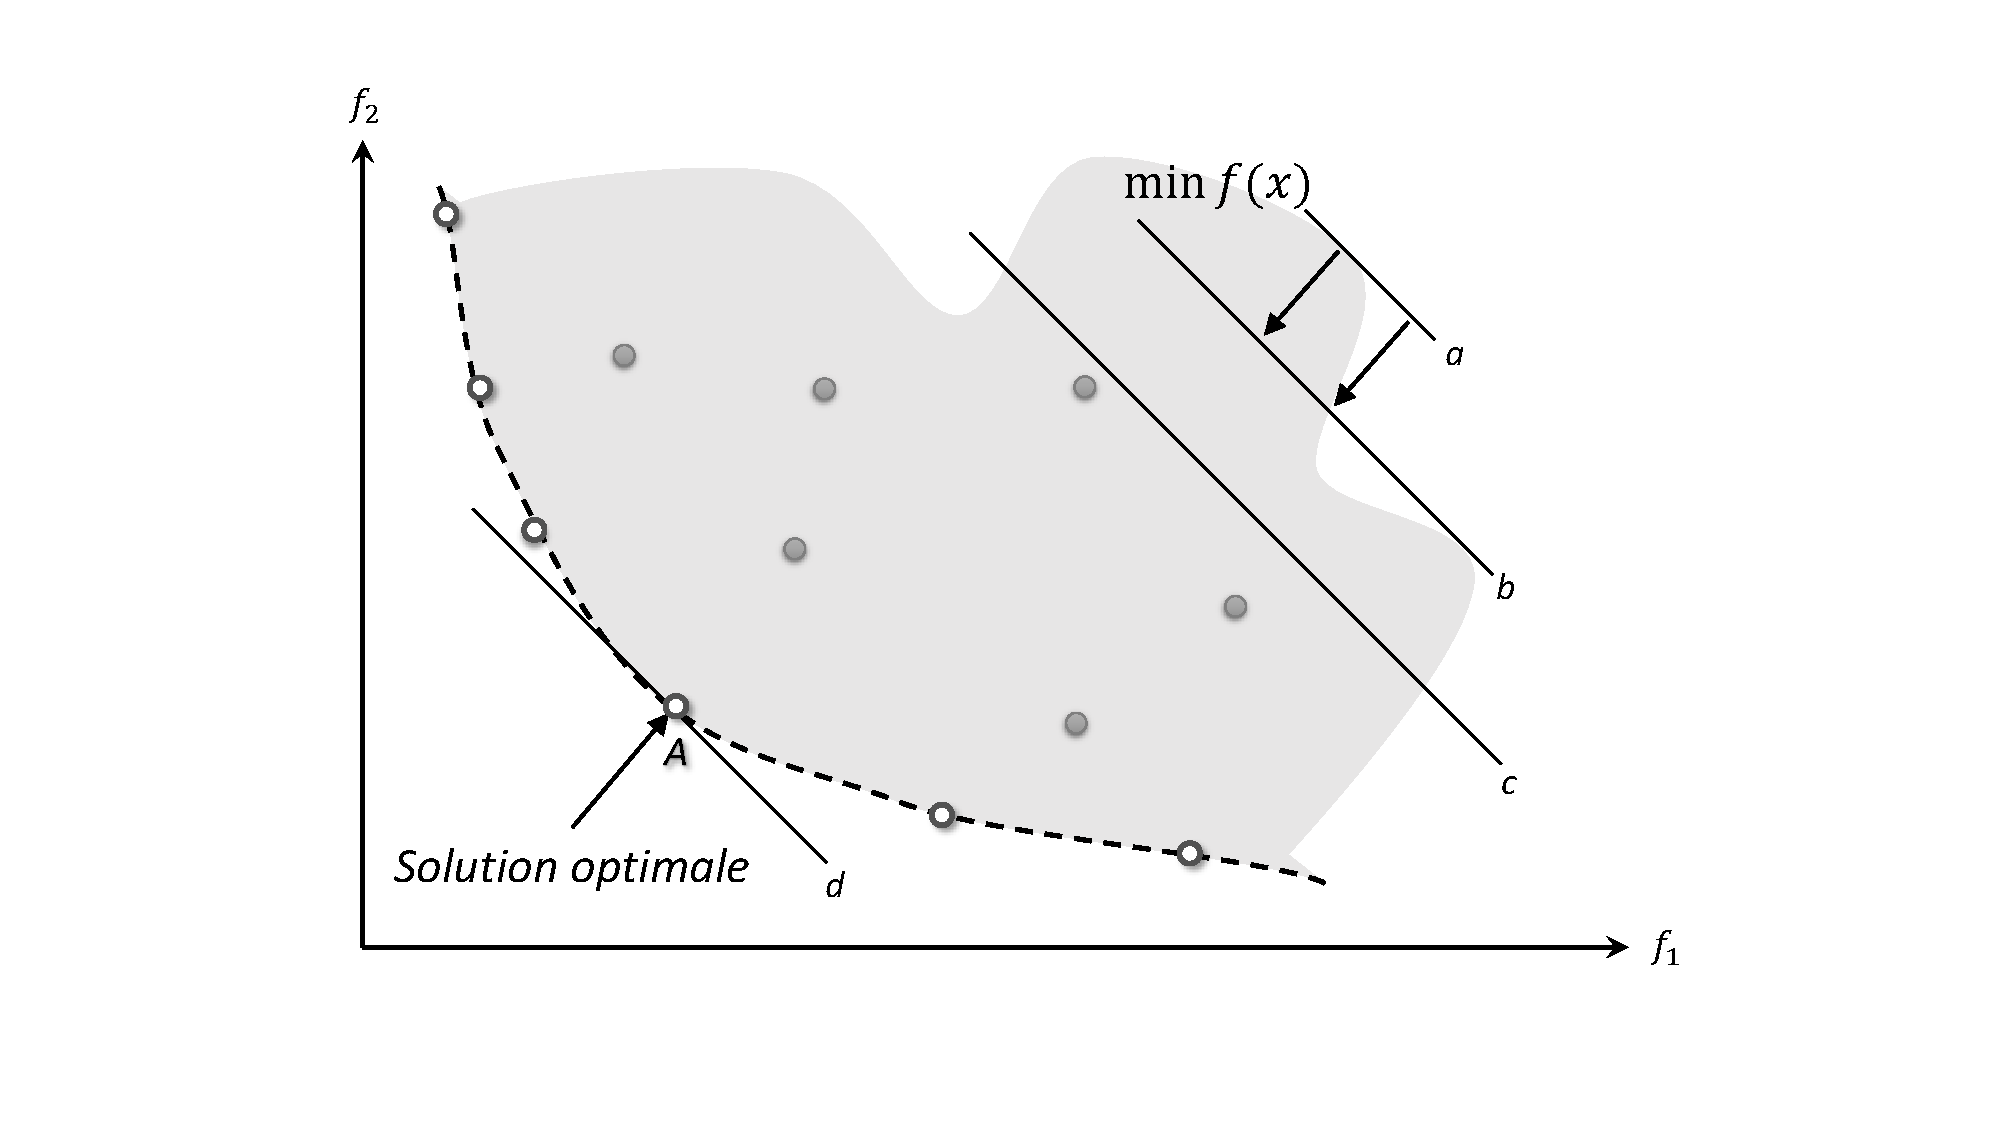
\includegraphics[scale=0.4]{chapitre2/chap2Fig/weighted-sum-ex.pdf}
\caption{Exemple de la méthode de pondération.}
 \label{fig:weighted-sum-ex}
\end{center}
\end{figure}

L’avantage de cette méthode est sa facilité d’implémentation et le fait qu’elle puisse être utilisée avec les méthodes et techniques définis pour $\mathcal{OMO}$. Cependant, comme mentionné précédemment, il est important dans $\mathcal{PMO}$ que les solutions d'optimum de Pareto soient générées et que toute solution puisse être trouvée. À cet égard, la méthode de pondération présente un sérieux défaut. La solution d'optimum de Pareto peut être trouvée en modifiant les poids seulement si le problème est convexe. Ainsi, il peut arriver que certaines solutions d'optimum de Pareto pour des problèmes non convexes ne puissent être trouvées, peu importe la façon dont les poids sont sélectionnés \cite{Branke08}. C'est le cas du point $A$ dans la \ref{fig:pareto-optimality}.


\paragraph{Méthode $\epsilon$-contrainte}
Afin d'atténuer les difficultés rencontrées par la méthode de somme pondérée dans la résolution de problèmes ayant des espaces objectifs non convexes, la méthode de $\epsilon$-contrainte est utilisée. L'idée de cette méthode est la transformation des $k-1$ fonctions objectives en contraintes. La fonction objective restante, qui peut être choisi arbitrairement, est la fonction objective du $\mathcal{OMO}$ résultant \cite{Haimes71,Vira83} :
\begin{alignat}{2}
& \text{minimiser} \quad && y = f(x) = f_h(x) \nonumber \\
& \text{avec}   \quad && e_i(x) = f_i(x) \leqslant \epsilon_i \quad (1 \leqslant i \leqslant k, i \neq h)  \nonumber \\
& \text{et}   \quad && x \in X_f
\end{alignat}
Les limites supérieures, $\epsilon_i$, sont les paramètres à varier afin de trouver des solutions d'optimum de Pareto. En pratique, il peut être difficile de spécifier les limites supérieures pour avoir des solutions aux problème $\mathcal{OMO}$, c'est-à-dire que la région réalisable ne soit pas vide. Cette difficulté est soulignée lorsque le nombre de fonctions objectives augmente \cite{Branke08}. Cependant, il est possible d'utiliser la méthode de manière a priori et demander au décideur de spécifier la fonction à optimiser et les limites supérieures.

\paragraph{Méthode programmation par but}
L'idée principale de la programmation par but est de trouver des solutions qui atteignent une cible prédéfinie pour une ou plusieurs fonctions objectives \cite{Charnes55}. Dans cette méthode, le décideur est invité à spécifier les niveaux cibles $z_i (i = 1, \cdots, k)$ pour les fonctions objectives. Ensuite, les écarts par rapport à ces niveaux cibles sont minimisés. Une fonction objective conjointement avec un niveau de cible est appelée un \textit{but}. Pour les problèmes de minimisation, les buts sont de la forme $f_i(x) \leqslant z_i$ et les niveaux de cibles sont supposés être sélectionnés. Après la formations des buts, les \textit{écarts} $\delta_i = max[0, f_i(x) - z_i]$ des valeurs de la fonction objective sont minimisés.

La méthode comporte plusieurs variantes. Dans l'approche de \textit{programmation par but pondérés} \cite{Charnes77}, la somme pondérée des écarts est minimisée. Cela signifie qu'en plus des niveaux de cibles, le décideur doit spécifier des poids positifs. Puis nous résolvons le problème :
\begin{alignat}{2}
& \text{minimiser} \quad && \sum_{i=1}^{k}\omega_i \delta_i \nonumber \\
& \text{avec}      \quad && f_i(x) - \delta_i \leqslant z_i \text{ et } \delta_i \geqslant 0  \nonumber \\
& \text{et}   \quad && x \in X_f
\end{alignat}

D'autre part, dans l'approche de \textit{programmation par but lexicographiques}, le décideur doit spécifier un ordre lexicographique pour les buts en plus des niveaux de cible. Après l'ordonnancement lexicographique, le problème des déviations en tant que fonctions objectives est résolu lexicographiquement \cite{Collette13}. Mentionnons également une approche de \textit{programmation par but min-max} où le maximum d'écarts est minimisé \cite{Deb01}.

\subsubsection{Méthodes évolutionnaires}
Les algorithmes évolutionnaires (\acrshort[hyper=false]{AE}) sont des méthodes de recherche inspirées de la nature pour résoudre des problèmes complexes avec un grand espace de recherche. Certaines caractéristiques de cette technique, tel que la possibilité de trouver des solutions optimales multiples dans une seule simulation, les rendent populaires et motivent les chercheurs à les utiliser dans divers domaines d'applications comme alternative aux méthodes classiques décrites précédemment.

Il existe plusieurs familles historiques d'algorithme évolutionnaires qui se sont développées de façon indépendante : la programmation évolutionnaire, les algorithmes génétiques, les stratégies d’évolutions et la programmation génétique.
Aujourd'hui, ces terminologies sont considérées comme sous-domaines des AE \cite{Branke08}.

Cette section vise à fournir un aperçu d'un certain nombre d'AE bien connus, conçus pour traiter des problèmes d'optimisation multi-objectifs, par la présentation du vocabulaire et le principe général de leurs fonctionnements.

\paragraph{Principe de fonctionnement}
En général, un AE se caractérise par trois faits :
\begin{enumerate}
 \item un ensemble de solutions candidates est maintenu, ce qui
 \item subit un processus de sélection, et qui
 \item est manipulé par les opérateurs génétiques, généralement le croisement et la mutation.
\end{enumerate}

Par analogie avec l'évolution naturelle, les solutions candidates sont appelées \textit{individus} et l'ensemble des solutions candidates s'appelle la \textit{population}. Chaque individu représente une solution possible, et il est codé sur la base d'une structure appropriée. Sans perte de généralité, on suppose que cette structure est un vecteur, par exemple un vecteur de bits ou un vecteur de valeur réelle. L'ensemble de tous les vecteurs possibles constitue \textit{l'espace des individus} $I$. Dans cette terminologie, la population est un ensemble de vecteurs $i \in I$.

Dans le processus de \textit{sélection}, qui peut être stochastique ou complètement déterministe, les individus de faible qualité sont retirés de la population, tandis que les individus de haute qualité sont reproduits. L'objectif est de concentrer la recherche sur des portions particulières de l'espace de recherche et d'augmenter la qualité moyenne au sein de la population. La qualité d'un individu par rapport à la tâche d'optimisation est représentée par une valeur scalaire, qui est le \textit{fitness}.

Le \textit{croisement} et la \textit{mutation} visent à générer de nouvelles solutions dans l'espace de recherche par la variation de celles existantes. L'opérateur de croisement prend un certain nombre de parents et crée un certain nombre d'enfants en recombinant les parents. Pour simuler la nature stochastique de l'évolution, une probabilité de croisement est associée à cet opérateur. En revanche, l'opérateur de mutation modifie les individus en changeant de petites parties dans les vecteurs associés selon un taux de mutation donné. L'opérateur de \textit{l'élitisme} assure que la nouvelle population garde que les meilleures solutions de la population actuelle.

Sur la base des concepts ci-dessus, l'évolution naturelle est simulée par un processus itératif de calcul. Premièrement, une population initiale est créée au hasard ou suivant un schéma. Ensuite, une boucle (\textit{génération}) comprenant les étapes : évaluation (affectation de fitness), sélection, croisement et/ou mutation est exécutée un certain nombre de fois fixé. À la fin, le meilleur individu(s) dans la population finale, ou trouvé pendant tout le processus d'évolution, est le résultat de l'AE.

\begin{algorithm}
\caption{Algorithme général d'AE}
\label{algo:ae-algo}
\begin{algorithmic}[1]
\Require  $T$ \Comment{nombre maximal de générations}
\Ensure $A$ \Comment{ensemble non-dominé}
\State
$t = 0$;
\State
$Initialisation(P_t)$;
\Repeat
    \State $Evaluation(P_t)$;
    \State $P_t^\prime = Selection(P_t)$;
    \State $P_t^{\prime\prime} = Croisement(P_t^\prime)$;
    \State $P_{t+1} = Mutation(P_t^{\prime\prime})$;
	\State $t = t+1$;
\Until{$Termination(P_t, P_{t+1})$;}
\State
\Return $A$;
\end{algorithmic}
\end{algorithm}

Dans l'\ref{algo:ae-algo}, la procédure de base d'un AE est donnée. La population $P$ à une certaine génération $t$ est représentée par le symbole $P_t$.

%Cependant, nous discutons la deuxième catégorie des algorithmes qui sont supposés être plus rapides et meilleurs que les algorithmes non élitistes \cite{Deb01}.
Les AE multi-objectifs (\acrshort[hyper=false]{AEMO}) peuvent être classés généralement en trois approches basées sur : \textit{la dominance}, \textit{la décomposition} et \textit{les indicateurs} \cite{Wagner07}. Dans les sections suivantes, nous les détaillons et nous présentons un algorithme représentatif de chaque approche.

% 3.3.1 EMO Principles book: Introduction to Multiobjective Optimization: Interactive Approaches
% Figure 1.1 Basic Evolutionary Algorithm’s Flowchart
\paragraph{Approches basées sur la dominance}
Les méthodes de cette catégorie se base sur le concept de la dominance de Pareto déjà introduit. Ils sont les approches les plus populaires dans la littérature, et ils existent depuis les deux dernières décennies. Les AEMO de cette catégorie peuvent être classés en deux groupes principaux : des algorithmes \textit{non-élitistes} et des algorithmes \textit{élitistes}. Comme décrit précédemment, l'élitisme est un mécanisme pour préserver les bons individus de la génération actuelle en les sauvant et en les transmettant à la génération suivante, ce qui accélère la convergence de la population vers le front de Pareto. Le premier groupe inclue : \textit{Non-Dominated Sorting Genetic Algorithm} (NSGA) \cite{Srinivas94},
\textit{Niched-Pareto Genetic Algorithm} (NPGA) \cite{Horn94}, \textit{Multi-Objective Genetic Algorithm} (MOGA) \cite{Fonseca93}, etc. Le deuxième groupe comprend : \textit{Elitist Non-Dominated Sorting Genetic Algorithm} (\acrshort[hyper=false]{NSGA-II}) \cite{Deb02}, \textit{Strength Pareto Evolutionary Algorithm} (SPEA-II) \cite{Zitzler01} et \textit{Pareto Envelope-based Selection Algorithm} (PESA-II) \cite{Corne01}, et plusieurs autres algorithmes.

\subparagraph{NSGA-II}
Un exemple classique de cette catégorie est NSGA-II par Deb \textit{et al} \cite{Deb02}. Cet algorithme génétique utilise une méthode de \textit{ranking} qui attribue aux solutions non-dominées de la population courante le meilleur score. Par la suite, les solutions qui ne sont dominées que par les solutions potentiellement efficaces, reçoivent le second meilleur score et ainsi de suite. De cette manière, la population est organisée en couches où chaque couche contient des solutions non comparables entre elles. Le ranking d’une population est illustré dans la \ref{fig:nsgaii-rank}. Dans cet exemple, les solutions $A$, $B$, $C$, $D$ reçoivent le rang 1 car elles ne sont dominées par aucune solution. Les solutions $E$, $F$ et $G$ ont le rang 2 car elles ne sont dominées que par des solutions de rang 1. Enfin, $H$ et $I$ sont affectées au rang 3. NSGA-II utilise aussi une seconde mesure, la distance de \textit{crowding}, visant à améliorer la diversité de la population du premier rang de l’espace des objectifs. La distance de crowding est une mesure permettant de déterminer le surpeuplement des individus du même front. Il s'agit d'une estimation de la densité de solutions qui entourent un individu. Comme le montre la \ref{fig:nsgaii-crowd}, la distance de crowding $d_i$ pour l'individu $C$ est définie comme un demi-périmètre de cuboïde formé par les individus voisins les plus proches de $C$ dans l'espace objectif (les points $B$ et $D$).

\begin{figure}
  \centering
  \subfloat[La méthode de \textit{ranking}.\label{fig:nsgaii-rank}]{
    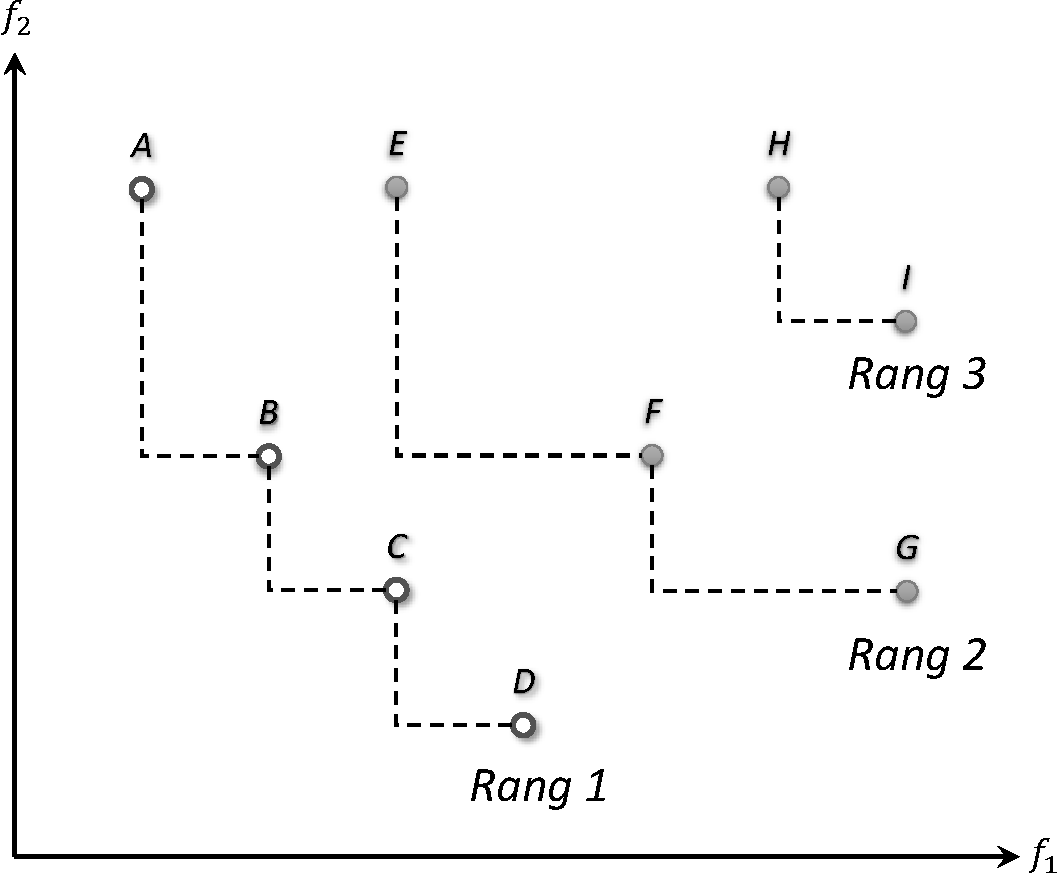
\includegraphics[scale=0.37]{chapitre2/chap2Fig/nsgaii-rank.pdf}
  }
  \quad
  \quad
  \subfloat[La méthode de la distance de \textit{crowding}.\label{fig:nsgaii-crowd}]{
    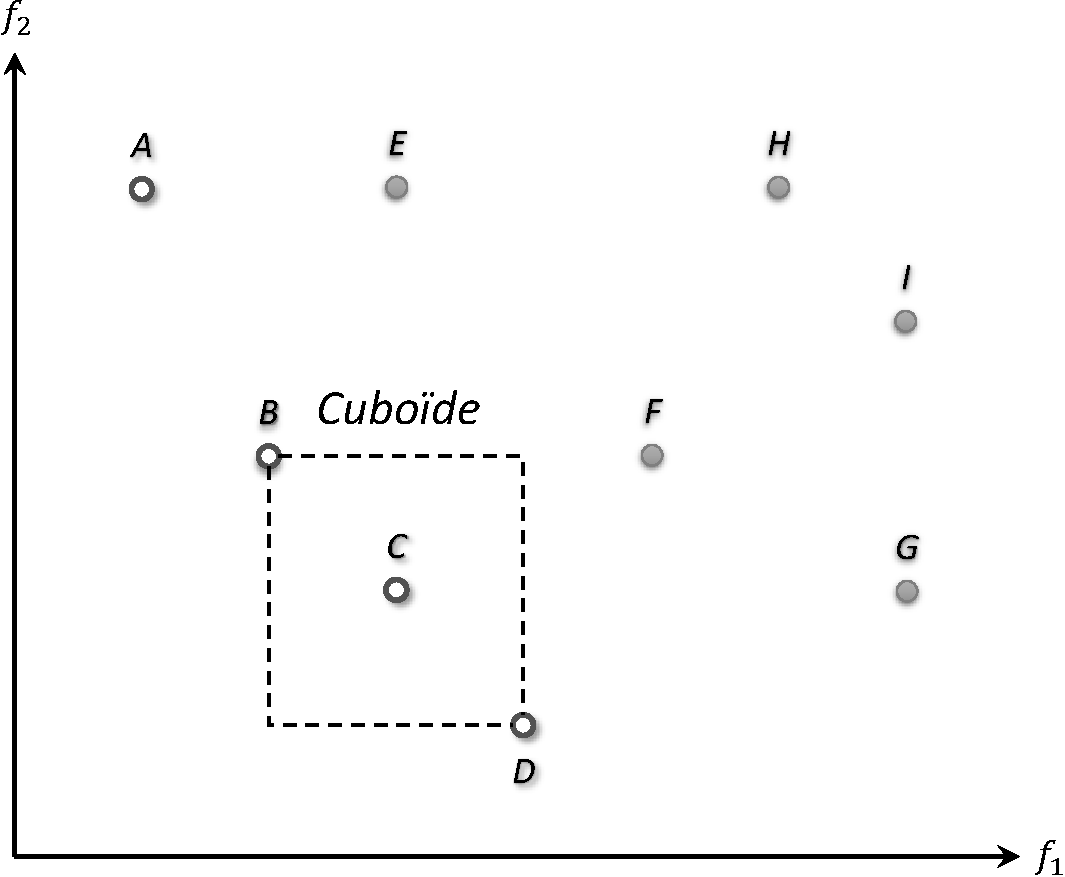
\includegraphics[scale=0.37]{chapitre2/chap2Fig/nsgaii-crowd.pdf}
  }
  \caption{Exemples des méthodes de NSGA-II.}\label{fig:nsgaii-example}
\end{figure}

\paragraph{Approches basées sur la décomposition}
Les méthodes basées sur la décomposition, connues aussi sous le nom d'approches d'agrégation pondérée, où un $\mathcal{PMO}$ est décomposé en un certain nombre de problèmes d'optimisation objectifs simples en utilisant un certain nombre de combinaisons de poids. Ces poids sont générés  soit de façon aléatoire \cite{Ishibuchi98}, soit dynamiquement et continuellement modifiées \cite{Jin01}, soit prédéfinies et uniformément réparties \cite{Murata01}. Parmi les algorithmes les plus courant : \textit{Multiple Single Objective Pareto Sampling} (MSOPS) \cite{Hughes03}, \textit{Multiobjective Evolutionary Algorithm based on Decomposition} (MOEA/D) \cite{Zhang07} et \textit{Repeated Single Objective} (RSO) \cite{Hughes05}.

\subparagraph{MOEA/D}
Cette variante récente d'algorithmes de décomposition a reçu une attention croissante en raison de sa simplicité de calcul et sa performance dans la recherche des solutions.
Le principe de cet algorithme est le suivant : Premièrement, il faut définir un $P$ vecteurs de poids uniformément distribués dans l’espace objectif. Ces vecteurs définissent des directions pour chercher les solutions. En effet, chaque vecteur de poids est utilisé pour définir un sous-problème mono-objectif en utilisant des fonctions scalaires comme la méthode de pondération ou la méthode de Tchebycheff. L’algorithme maintient également une population de solutions de taille $P$. Une solution est alors attachée à chaque fonction scalaire.

Le but de MOEA/D est de trouver les meilleures solutions par rapport à chacun des vecteurs de direction à l'aide de \textit{la notion de voisinage}. Étant donné un vecteur de direction $\lambda_i$ et le sous-problème scalaire sous-jacent pour tout $i \in \{1, \cdots, P\}$. L'algorithme définit l’ensemble $B(i)$ des voisins de $i$ comme étant les sous-problèmes correspondant aux vecteurs de direction les plus proches de $\lambda$. L’algorithme parcourt les sous-problèmes de façon itérative, et pour chacun, deux solutions parmi les voisins sont sélectionnées. Ces solutions permettent alors de produire une nouvelle solution, notée $y^\prime$, en utilisant des opérateurs de variations (mutation, croisement). La nouvelle solution $y^\prime$ est comparée aux solutions des voisins. Si $y^\prime$ permet d’améliorer la solution d’un voisin alors elle remplace cette solution et ainsi de suite pour tous les voisins. Ce mécanisme est répété pour toutes les directions jusqu’à ce qu’une condition d’arrêt soit satisfaite. A la fin, l’ensemble des solutions calculées par rapport à toutes ces directions est alors retourné en sortie.

\paragraph{Approches basées sur les indicateurs}
Une idée différente est d'attribuer un fitness aux individus basé sur un indicateur de performance pour évaluer la qualité, la convergence et la diversité des individus de la population. L'indicateur de \textit{l'hypervolume} \cite{Zitzler99b}, qui mesure le volume de la portion faiblement dominée par un ensemble de point dans l’espace objectif, a été largement adopté par les différents AEMO basés sur les indicateurs de performance. Cela est dû à sa précision et la diversité des ensembles de solutions non-dominées produits \cite{Wagner07}. Parmi les algorithmes proposés dans cette catégorie : \textit{Indicator-based Evolutionary Algorithm} (IBEA) \cite{Zitzler04} qui utilise une métrique de performance binaire comme indicateur, \textit{S-metric Selection-EMOA} (SMS-EMOA) \cite{Beume07} qui utilise l'indicateur d'hypervolume et plus récemment le \textit{Hypervolume Estimation Algorithm for Multiobjective Optimization} (HypE) \cite{Bader11} qui adopte la simulation Monte Carlo pour approximer la valeur exacte de l'hypervolume. Le principal défi de cette classe d'AEMO est la complexité élevée pour calculer l'indicateur de performance, en particulier lorsque le nombre d'objectifs est élevé \cite{Beume09}.

\subparagraph{IBEA}
L’idée principale de IBEA \cite{Zitzler04} est de formaliser les préférences entre individus en utilisant un indicateur de performance binaire de qualité $I$ arbitrairement choisi. Ensuite, chaque individu $x^1$ est attribué une valeur de fitness $F(x^1)$ correspondant à la mesure de la << perte en qualité >> si cet individu avait été retiré de la population $P$.
\begin{equation}
 F^\prime(x^1) = \sum_{x^2 \in P\setminus \{x^1\}} I(\{x^1\},\{x^2\})
\end{equation} 
Les auteurs proposent une autre formule modifiée qui amplifie l’influence des solutions non-dominées sur les solutions dominées. En d'autre terme, donner le plus grand score possible à une solution selon sa contribution par rapport aux autres solutions de la population.
\begin{equation}
 F(x^1) = \sum_{x^2 \in P\setminus \{x^1\}} - e^{-I(\{x^1\},\{x^2\})/k}
\end{equation}
Où $k > 0$ est un facteur d'échelle qui dépend de l’indicateur $I$ utilisé (par exemple, l'hypervolume ou epsilon) et du problème à optimiser.

\begin{figure}
\footnotesize
\begin{center}
\tikzset{
  basic/.style  = {draw, text width=4cm, drop shadow, rectangle},
  root/.style   = {basic, rounded corners=2pt, thin, align=center,
                   fill=green!30},
  level 2/.style = {basic, rounded corners=6pt, thin,align=center, fill=green!60,
                   text width=8em},
  level 3/.style = {basic, thin, align=left, fill=pink!60, text width=8.5em}
}

\begin{tikzpicture}[
  level 1/.style={basic,rounded corners=6pt, thin,align=center, fill=green!60,
                   text width=8em,sibling distance=97mm},
  level 2/.style = {basic, rounded corners=6pt, thin,align=center, fill=green!60,
                   text width=8em,sibling distance=50mm},
  level 3/.style = {basic, thin, align=left, fill=pink!60, text width=6.5em,sibling distance=40mm},
  edge from parent/.style={->,draw,black},
  >=latex]

% root of the the initial tree, level 1
\node[root] {Méthodes de résolution des $\mathcal{PMO}$}
% The first level, as children of the initial tree
  child {node[level 1] (c1) {Classiques}}
  child {node[level 1] (c2) {AEMO basés sur}
	  child {node[level 2,xshift=5pt] (c21) {La dominance}
		child {node[level 2,xshift=10pt] (c211) {Non-élitistes}}
		child {node[level 2,xshift=-10pt] (c212) {Élitistes}}
	  }
	  child {node[level 2] (c22) {La décomposition}}
	  child {node[level 2,xshift=-50pt] (c23) {Les indicateurs}}
  };

% The second level, relatively positioned nodes
\begin{scope}[every node/.style={level 3}]
\node [below of = c1, xshift=10pt, yshift=-5pt] (c11) {Pondération \cite{Gass55,Zadeh63}};
\node [below of = c11, yshift=-5pt] (c12) {$\epsilon$-contrainte \cite{Haimes71,Vira83}};
\node [below of = c12, yshift=-5pt] (c13) {Program. par but \cite{Charnes55,Charnes77}};

\node [below of = c211, xshift=10pt] (c2111) {NSGA \cite{Srinivas94}};
\node [below of = c2111] (c2112) {NPGA \cite{Horn94}};
\node [below of = c2112] (c2113) {MOGA \cite{Fonseca93}};

\node [below of = c212, xshift=10pt] (c2121) {NSGA-II \cite{Deb02}};
\node [below of = c2121] (c2122) {SPEA-II \cite{Zitzler01}};
\node [below of = c2122] (c2123) {PESA-II \cite{Corne01}};

\node [below of = c22, xshift=10pt] (c221) {MSOPS \cite{Hughes03}};
\node [below of = c221] (c222) {MOEA/D \cite{Zhang07}};
\node [below of = c222] (c223) {RSO \cite{Hughes05}};

\node [below of = c23, xshift=10pt] (c231) {IBEA \cite{Zitzler04}};
\node [below of = c231] (c232) {SMS-EMOA \cite{Beume07}};
\node [below of = c232] (c233) {HypE \cite{Bader11}};

\end{scope}

% lines from each level 1 node to every one of its "children"
\foreach \value in {1,...,3}
  \draw[->] (c1.178) |- (c1\value.west);

\foreach \value in {1,...,3}
  \draw[->] (c211.178) |- (c211\value.west);
  
\foreach \value in {1,...,3}
  \draw[->] (c212.178) |- (c212\value.west);
  
\foreach \value in {1,...,3}
  \draw[->] (c22.178) |- (c22\value.west);
  
\foreach \value in {1,...,3}
  \draw[->] (c23.178) |- (c23\value.west);
\end{tikzpicture}
\caption{Classification des méthodes de résolutions d'un $\mathcal{PMO}$.}
\label{fig:pmo-classification}
\end{center}
\end{figure}

La \ref{fig:pmo-classification} montre les différentes méthodes de résolution d'un $\mathcal{PMO}$ discutées dans cette section.

\subsection{Optimisation multi-objectifs dans les bases de données}
Nous passons maintenant sur l'application des techniques d'optimisation multi-objectifs décrites dans la section précédente dans le contexte des bases de données. En étudiant les travaux de littérature, nous trouvons que les techniques d'optimisation multi-objectifs ont été largement employées pour résoudre des problèmes diverses dans les base de données sur plusieurs niveaux : le Cloud Computing (ex: minimisation des coûts monétaire) \cite{Kong12,Dokeroglu14,Helff16}, les bases de données temps réel (ex: ordonnancement de requêtes) \cite{Thiele09,Zhao16}, la conception physique des bases de données (ex: le problème de sélection d'index \cite{Bruno11b,Bruno08}, la fragmentation \cite{Bellatreche13b,Bellatreche13c,Barr13}, les vues matérialisées \cite{Lawrence06,Talebian13,Goswami13}), le traitement de requête \cite{Papadimitriou01,Trummer14,Borzsony01}, etc.

Cependant, nous allons focaliser notre étude sur les vues matérialisées et la phase de traitement des requêtes par un SGBD.

\subsubsection{$\mathcal{PSV}$ multi-objectifs}
% 2.15 Multi-Objective View Selection Problem
% 3 papers: A Lexicographic Ordering Genetic Algorithm for Solving Multi-objective View Selection Problem
% Multiobjective Genetic Algorithms for Materialized View Selection in OLAP Data Warehouses
% Multiobjective Differential Evolution Algorithm Using Binary Encoded Data in Selecting Views for Materializing in Data Warehouse
Le $\mathcal{PSV}$ discuté dans le \ref{sec:psv} (ou une autre structure d'optimisation en général) peut être reformulé pour sélectionner un ensemble de vues avec plusieurs objectifs à optimiser en même temps. En effet, dans les travaux qui se basent sur l'optimisation mono-objectif, seul le coût de traitement de requête est considéré comme fonction objectif. Cependant, le coût de stockage ou de maintenance ont été considérés comme des contraintes à satisfaire.

En analysant les travaux de littérature, la première formalisation de $\mathcal{PSV}$ multi-objectif a été proposée dans \cite{Lawrence06}, dans lequel le temps de réponse de requête et le temps de maintenance doivent être minimisés simultanément sous la contrainte d'espace de stockage. La structure de représentation de données employée est la technique de cube treillis. Dans ce but, deux AEMO non-élitistes, MOGA et NPGA ont été adoptés pour résoudre le problème de sélection de vue. Pour faire face aux contraintes, l'auteur a proposé deux méthodes. La première méthode intègre la contrainte dans l'objectif et définit la notation de dominance de telle sorte qu'un individu infaisable est toujours dominé par un individu réalisable. La seconde permet à un individu infaisable d'être crée et d'utiliser une fonction de réparation pour le convertir en un faisable. Les résultats d'expérimentations sur des ensembles de données réelles et synthétiques montrent que les AEMO sont très compétitifs par rapport aux algorithmes de glouton classique.

Les auteurs de \cite{Talebian13} ont proposé un algorithme génétique basé sur le poids (WBGA) pour résoudre le problème de sélection de vue. L'objectif est de minimiser la somme pondérée du temps de réponse de requêtes et du temps de maintenance en fonction de la contrainte d'espace de stockage. Le cube treillis été utilisé comme structure de données. Le WBGA multiplie chaque objectif $i$ à un facteur de poids correspondant $w_i$ pour calculer une valeur de fitness. Contrairement à l'approche de la somme pondérée classique avec des poids fixes, la WBGA utilise le mécanisme d'optimisation génétique pour rechercher des solutions avec des poids différents en parallèle. Par conséquent, la population converge vers un ensemble de solutions optimales avec différents vecteurs de poids en un seul passage.

Dans \cite{Goswami13}, les auteurs ont mis en œuvre un algorithme à évolution différentielle (ED) multi-objectifs pour résoudre le $\mathcal{PSV}$ dans un entrepôt de données. Le temps de réponse et le coût de maintenance sont considérés comme fonctions objectifs, tandis que l'espace de stockage comme contrainte. Les solutions candidates sont représentées par la structure de MVPP. L'algorithme ED est une méthode méta-heuristiques stochastiques d'optimisation des espaces continus. La technique s'avère appropriée pour sélectionner des solutions représentatives à partir d'un grand nombre de solutions non-dominantes du $\mathcal{PSV}$.

% Approximation Schemes for Many-Objective Query Optimization
\subsubsection{Traitement de requêtes multi-objectifs}
Il existe souvent d'autres indicateurs de coûts en plus du temps d'exécution qui sont pertinents pour comparer les plans de requêtes, tel que le coût d'argent dans un scénario de Cloud Computing par exemple.
Les travaux qui implémentent les techniques d'optimisation multi-objectifs dans le contexte du traitement de requêtes peuvent être divisés en deux catégories. La première catégorie considère le niveau d'optimisation de requêtes, afin de produire des plans d'exécutions respectant les objectifs prédéfinis. D'autre part, la deuxième catégorie considère le niveaux données ou requêtage, en cherchant dans les données et produisant des résultats suivant les objectifs. Nous citons les travaux de chaque catégorie dans les sections suivantes.

\paragraph{Optimisation de requêtes}
L'optimisation de requêtes multi-objectifs modélise le coût d'un plan de requête comme un vecteur de coût où chaque composante vectorielle représente le coût selon une métrique de coût différente. L'optimisation classique des requêtes peut être considérée comme un cas particulier d'optimisation de requête multi-objectif où la dimension de l'espace de coût est égale à un (c'est-à-dire le nombre de composantes de vecteur de coût).

Différentes métriques de coût peuvent entrer en conflit. Par conséquent, l'objectif de l'optimisation est de trouver un plan de requête qui réalise le meilleur compromis entre les différentes métriques de coûts. Le meilleur compromis dépend des préférences de l'utilisateur fournies en entrée à l'optimiseur (par exemple, un utilisateur peut définir des pondérations entre différentes métriques de coûts pour exprimer une importance relative ou définir des bornes supérieurs/inférieurs de coût).

Le travail de \cite{Papadimitriou01} présente un algorithme d'approximation multi-objectifs pour exécuter des opérateurs d'une requête vers des sites dans le cas d'une base de données distribuée. Il suppose que chaque site soumet une << offre >> pour la requête, en spécifiant un délai pour la délivrance du résultat et un coût monétaire associé. L'optimiseur de requêtes compare alors ces offres à un compris entre le coût/délai fourni par l'utilisateur (une fonction $u(d)$, qui spécifie pour chaque valeur $d$ du délai, le montant d'argent que l'utilisateur est prêt à payer afin de recevoir les résultats de la requête dans le temps $d$) et tente de déterminer la combinaison des exécutions de la sous-requête qui maximise les préférences de l'utilisateur. Les auteurs proposent un algorithme glouton et une preuve mathématique pour résoudre ce problème.

Les auteurs de \cite{Fan06} ont proposé un framework de traitement des requêtes pour l'intégration des données. Ils considèrent la couverture, la densité et la latence des sources de donnée comme des fonctions objectives, et ils ont développé un modèle de coût pour estimer chacun d'entre eux.
Dans la phase d'optimisation, ils ont utilisé une méthode de pondération pour combiner les fonctions objectives en une seule fonction agrégée, en utilisant des paramètres de poids permettant à l'utilisateur de changer l'importance relative associée aux différents objectifs. Les expérimentations montrent que le modèle de coût est capable d'estimer efficacement chaque type d'objectif, et la procédure d'optimisation est capable de faire des compromis flexibles entre les objectifs lors du traitement des requêtes.

Les travaux récents de Trummer et Koch traitent le problème d'optimisation de requêtes ayant plusieurs objectifs (\textit{many-objective}). Grâce à l'avancement de la technologie de matériel informatique, les auteurs ont proposé de revisiter les suppositions faites par les chercheurs lors du développement des méthode d'optimisation de requêtes les premiers jours, afin d'exploiter les capacités logicielles et matérielles actuelles. Ils ont présenté le problème d'optimisation de requête multi-objectif où les plans de requêtes sont comparés selon plusieurs métriques de coût, comme par exemple le temps d'exécution, les frais monétaires, les mesures de consommation de ressources système (le nombre de noyaux utilisés, la quantité d'espace mémoire consommée). Les techniques utilisées pour résoudre ce problème inclues : des schémas d'approximation qui permettent de relaxer progressivement l'optimalité d'un plan pour accélérer le processus d'optimisation \cite{Trummer14b}, un algorithme incrémental qui divise l'optimisation en plusieurs petites étapes progressives, permettant aux utilisateurs de guider l'algorithme après chaque étape, ce qui rend de l'optimisation des requêtes un processus interactif \cite{Trummer15}, une optimisation de requêtes paramétrée, avec l'introduction d'une étape de pré-traitement si les requêtes correspondent à des modèles de requêtes connus à l'avance \cite{Trummer14}, une approche de décomposition qui permet de paralléliser l'optimisation de requêtes classique sur des clusters de grande taille avec des centaines de nœuds \cite{Trummer16}, l'utilisation d'un algorithme aléatoire (un Hill Climbing modifié) pour l'optimisation de requêtes multi-objectif qui est capable de traiter des requêtes avec des centaines de jointures \cite{Trummer16b}, la transformation du problème d'optimisation de requêtes en un programme linéaire en nombres entiers mixtes qui permet d'appliquer des solveurs de la programmation en nombres entiers pour traiter des espaces de recherche plus grands \cite{Trummer15b}, et enfin, ils ont présenté des résultats d'expérimentations pour résoudre le problème d'optimisation de requêtes sur l'ordinateur quantique D-Wave 2X avec plus de 1000 qubits (100 millions de fois plus rapide qu'un ordinateur classique) \cite{Trummer16c}.

\paragraph{L'opérateur Skyline}
L'opérateur Skyline est utilisé dans une requête et effectue un filtrage des résultats à partir d'une base de données afin qu'il ne conserve que les objets qui ne sont pas dominés par les autres.

Cet opérateur est une extension de SQL proposée par Börzsönyi \textit{et al.} \cite{Borzsony01}. Un exemple classique d'application de l'opérateur Skyline implique de choisir un hôtel pour des vacances. L'utilisateur veut que l'hôtel soit à la fois bon marché et proche de la plage. Cependant, les hôtels qui sont près de la plage peuvent également être coûteux. Dans ce cas, l'opérateur Skyline ne présenterait que les hôtels qui ne sont pas pires que tout autre hôtel à la fois dans le prix et la distance.
Dans le cas d'un ensemble de données composé d'objets multidimensionnels, un objet domine un autre objet s'il est aussi bon dans toutes les dimensions et mieux dans au moins une dimension \cite{Tiakas15}.

\begin{example}
 Börzsönyi \textit{et al.} ont proposé la syntaxe suivante pour l'opérateur Skyline \cite{Borzsony01} :
 %\begin{verbatim}
 \begin{lstlisting}[language=Sql]
  SELECT ... FROM ... WHERE ...
  GROUP BY ... HAVING ...
  SKYLINE OF [DISTINCT] d1 [MIN | MAX | DIFF],
                 ..., dm [MIN | MAX | DIFF]
  ORDER BY ...
 \end{lstlisting}
 %\end{verbatim}
 Où $d_1, \cdots d_m$ désignent les dimensions de Skyline et \texttt{MIN}, \texttt{MAX} et \texttt{DIFF} spécifient si la valeur de cette dimension doit être minimisée, maximisée ou simplement la différence.
\end{example}

L'opérateur Skyline peut être implémenté directement dans SQL en utilisant des instructions SQL courantes, mais cela s'est avéré être très lent \cite{Borzsony01}. D'autres algorithmes qui utilisent la méthode diviser pour régner, les indexes \cite{Borzsony01}, MapReduce \cite{Mullesgaard14} et calcul généraliste sur les cartes graphiques \cite{Bogh13} ont été proposés. Les requêtes Skyline sur les flux de données ont été étudiées dans le contexte du traitement parallèle des requêtes sur des systèmes multi-cœurs, en raison de leur large utilisation dans les problèmes de prise de décision en temps réel et les analyses de flux de données \cite{De16}.
Une étude récente et détaillée sur les différentes techniques d'implémentation du l'opérateur Skyline peut être trouvée dans \cite{Tiakas15}.

\subsection{Bilan et discussion}
Nous avons présenté dans cette section le problème de d'optimisation multi-objectifs, sa formulation et ses méthodes de résolution. Nous avons détaillé en particulier la méthode de la somme pondérée et les algorithmes NSGA-II, MOEA/D et IBEA car ils sont les plus populaires. De plus, nous avons cité les principaux travaux qui appliquent ce concept dans les bases de données, en particulier sur le problème de sélection de vues et le traitement de requêtes.

Dans notre étude, l'intégration du nouveau besoin non-fonctionnel qui est l'énergie dans la base de données, est considéré comme une fonction objective à optimiser. De ce fait, nous proposons de reformuler le problème de sélection des structures d'optimisations et le traitement de requête en un problème multi-objectifs, où il faut optimiser deux objectifs : le temps d'exécution de la charge de requêtes et la consommation d’énergie, avec la prise en compte des contraintes telles que le coût de maintenance et l'espace de stockage. Pour résoudre ce nouveau problème, il faut (1) proposer un modèle de coût qui permet de calculer la fonction objectif d'énergie, (2) adopter une méthode de prise de décision pour avoir un compromis entre la performance et l'énergie (une méthode a priori, interactive ou a posteriori), et (3) choisir la bonne configuration d'algorithme et des paramètres pour résoudre le $\mathcal{PMO}$.

\section{Conclusion}\label{sec:Conclusion}
Afin d'intégrer l'énergie dans une base de données, il faut, en premier lieu, l'étudier pour identifier ses composantes qui peuvent avoir un impact sur la consommation énergétique du système. Dans ce chapitre nous avons décrit l'ensemble des phases traditionnelles de cycle de vie de conception d’une base de données : l’analyse de besoins, la modélisation conceptuelle, logique, physique et le déploiement. Nous avons identifié l’opportunité d'intégrer l'énergie dans la phase de conception physique, plus précisément, dans le choix d'une structure d'optimisation. Nous nous sommes focalisés sur la technique redondante qui est les vues matérialisées, et nous avons proposé de reformuler le problème de sélection de vues en un problème multi-objectifs ou il faut minimiser le temps de réponse et la consommation d'énergie en respectant certaines contraintes. Nous avons également cité les travaux d'état de l'art qui traitement le $\mathcal{PSV}$ en version mono et multi-objectifs.

En seconde lieu, nous avons étudier la phase de traitement de requêtes dans un SGBD relationnel, qui inclue : la phase d'analyse, la transformation, la génération de plans et optimisation et enfin l'exécution. Cette étude nous a permis d'identifier les paramètres clés qu'il faut prendre en considération lors de conception d'un optimiseur de requêtes éco-énergétique. Ces paramètres incluent un modèle de coût pour estimer la consommation d'énergie d'une requête SQL et une technique d'intégration de ce modèle de coût dans la phase de génération de plans. En parallèle à la description des composantes d'un moteur de traitement de requête, nous avons passé en revue les principaux techniques et travaux proposés dans l'état de l'art.

En troisième lieu, nous avons focalisé notre attention sur les problèmes d'optimisation multi-objectifs. Car notre nouveau problème d'incorporation de l'énergie nécessite une reformulation multi-objectifs, afin de proposer aux utilisateurs et administrateurs de base de données un ensemble de solutions avec des compromis variés. Nous avons présenté la formulation des $\mathcal{PMO}$, ses principales méthodes de résolutions : classiques et évolutionnaires, et la démarche à suivre pour intégrer ces méthodes par rapport à l'utilisateur (méthode a priori, interactive ou a posteriori).

Dans le prochain chapitre, nous allons présenter le concept d'énergie, ses propriétés, et un état de l'art sur les travaux de minimisation d'énergie dans les systèmes informatiques.

\chapter{L'énergie dans les systèmes informatiques}
\label{chap3}

\epigraph{<< With out passion you don't have energy, with out energy you have nothing. >>}{--- \textup{Donald Trump}}

\NoChapterPrefix \NoChapterNumberInRef {\hypersetup{linkcolor=black} \minitoc}

%% numérotation des figures, des tables et des équations préfixé par le numéro de chapitre
\makeatletter
\renewcommand{\thefigure}{\ifnum \c@section>\z@ \thechapter.\fi
 \@arabic\c@figure}
\@addtoreset{figure}{chapter}
\makeatother

\makeatletter
\renewcommand{\thetable}{\ifnum \c@section>\z@ \thechapter.\fi
 \@arabic\c@table}
\@addtoreset{table}{chapter}
\makeatother

\makeatletter
\renewcommand{\theequation}{\ifnum \c@section>\z@ \thechapter.\fi
 \@arabic\c@equation}
\@addtoreset{equation}{chapter}
\makeatother
%%-----------------------------------------------------------------
%% Résumé
%%-----------------------------------------------------------------


%laisser une page ou deux pages vides, telle est la question !
%\EmptyNewPage
\newpage

%********************************************************************************
%********************************************************************************
\section{Introduction}
% \section{Conception des modèles de coût}
% \subsection{Définition et évolution}
% \subsection{Conception des modèles de coût}
% \subsubsection{Identification des paramètres et des formules}
% \subsubsection{Calibration et apprentissage automatique}
% \subsubsection{Évaluation (mesure d'énergie : niveau système, niveau composant)}
La demande croissante de traitement de l'information a entraîné la demande de systèmes de gestion de données plus économiques, plus rapides et plus vastes. En le même temps, une part importante et croissante du coût total de propriété de ces systèmes sont l'énergie et le refroidissement. Ces dernières années, l'augmentation des coûts de l'énergie est devenue l'une des questions cruciales dans les centres de données. La nouvelle approche qui s'oriente vers les technologies de préservation de l'énergie a vu l'apparition et l'émergence des concepts tels que les systèmes éco-énergétiques. Par conséquent, l'objectif des concepteurs du système informatique est allé vers la puissance électrique et l'efficacité énergétique. 

Toutefois, pour résoudre à la fois le problème énergétique des centres de données tout en continuant à alimenter la demande des ressources en matière de gestion des données, nous devrons passer de l'optimisation des systèmes de gestion des données aux performances pures à l'optimisation de l'efficacité énergétique.
Les bases de données constituent une grande partie des ressources dans un centre de données, et consomment ainsi une large partie d'énergie. Traditionnellement, les recherches antérieures se sont uniquement concentrées sur l'amélioration des caractéristiques de performance des bases de données au cours des phases de conception et d’exploitation. Le \textit{modèle standard} a pour but de maximiser les performances du SGBD ou, en d'autres termes, de minimiser les temps de réponse lors de l'exécution des requêtes. Cependant, les BDs n'ont pas la capacité de gérer la consommation d'énergie lors de son fonctionnement. Contrairement à l'approche traditionnelle, le \textit{modèle éco-énergétique}, introduit dans ce chapitre, utilise l'\textit{efficacité énergétique} comme étant un aspect supplémentaire qui devrait être considéré dans le processus interne du SGBD.

Pour identifier les défis ouverts dans ce domaine et faciliter des futurs progrès, il est essentiel de synthétiser et classer les recherches sur la conception éco-énergétique réalisées à ce jour. Ce chapitre traite le problème de la consommation de l'énergie et présente ainsi une taxonomie des travaux sur la conception économe en énergie des systèmes informatiques couvrant les niveaux : matériels, systèmes d'exploitations, applications et bases de données.

% Le reste de ce chapitre est organisé comme suit. Dans la section suivante, les modèles de puissance et d'énergie sont présentés. La section 2.3 traite des problèmes causés par la consommation élevée d'énergie et d'énergie. Les sections 2.4.1-2.4.4 présentent la taxonomie et l'enquête de la recherche sur la conception éconergétique des systèmes informatiques. Le chapitre se termine avec le positionnement de la thèse actuelle dans le domaine de la recherche à la section 2.5, suivi d'un résumé et des orientations pour les travaux futurs de la section 2.6.

\section{L'énergie dans la technologie de l'information}
Dans cette section, nous mettons en avant le problème de l'efficacité énergétique et nous décrivons certaines façons possibles permettant de l'aborder.

\subsection{Le concept de l'énergie}
Pour faciliter la compréhension du reste de notre thèse, certains concepts et définitions préliminaires sont donnés. Le mot << énergie >> vient du grec \textbf{energeia} signifiant << \textit{\textbf{force en action}} >> \cite{Bowers00}, cette terminologie vient d'une approche physique du problème, décrivant l'énergie comme \cite{Ronneau04}:
\begin{definition}
L'énergie est une mesure de la capacité d'un système à modifier un état, à produire un travail entraînant un mouvement, un rayonnement électromagnétique ou de la chaleur.
\end{definition}
L'énergie peut exister sous diverses formes telles que l'énergie mécanique, l'énergie thermique, l'énergie de la lumière, l'énergie sonore, l'énergie magnétique, l'énergie électrique, l'énergie chimique et l'énergie nucléaire. Nous focalisons sur l'énergie électrique.
Le transfert d’énergie en une seconde est défini comme la puissance électrique. Plus précisément :
\begin{definition}
La puissance est la quantité d'énergie d'un système par unité de temps, ou le rythme de faire un travail.
\end{definition}
L'énergie est généralement mesurée en \textit{Joules} tandis que la puissance est mesurée en \textit{Watts}. Formellement, l'énergie et la puissance peuvent être définies comme suit:
\begin{equation}\label{eq:power}
 P = \frac{W}{t}
\end{equation}
\begin{equation}\label{eq:energy}
 E = P \times t
\end{equation}
où $P$, $t$, $W$ et $E$ représentent respectivement, une puissance, une période de temps, le travail total effectué dans ce laps de temps, et de l'énergie. Ces concepts de puissance, travail et énergie sont utilisés différemment dans divers contextes. Dans le contexte de la technologie d'information, le travail implique des activités associées à l'exécution de programmes (par exemple : addition, soustraction ou opération dans la mémoire), la puissance est le taux pour lequel l'ordinateur consomme de l'énergie électrique (ou la dissipe sous forme de chaleur) et l'énergie est l'énergie électrique totale que consomme l'ordinateur (ou se dissipe en chaleur) au fil du temps \cite{Venkatachalam05}.

Cependant, l'énergie peut être réduite soit par la minimisation du laps du temps ou de la puissance consommée.
En général, la consommation de la puissance électrique d'un système donné peut-être divisée en deux parties :
\begin{enumerate}
\item \textit{Puissance de base}: La consommation de la puissance lorsque le système est inactif. Cela inclut la consommation des ventilateurs, processeur, mémoire, périphériques d'E/S et les autres composants de la carte mère dans un état d'inactivité.
\item \textit{Puissance active}: La consommation de la puissance lors de l'exécution d'une charge de travail. Les composants qui influencent sur la puissance active sont déterminés par le type de charge de travail qui s'exécute sur la machine, et la façon avec laquelle elle utilise le processeur, la mémoire et les dispositifs d'E/S.
\end{enumerate}
Deux concepts de puissance électrique doivent être pris en considération lors de l'évaluation de l'utilisation d'énergie dans un système : \textit{la puissance moyenne} représentant la puissance moyenne consommée au cours d'exécution de la charge de requête, et \textit{le pic} représentant la puissance maximale (\textit{peak power}). Dans cette thèse, nous traitons la puissance moyenne.

Lorsqu'on évoque des économies de l'énergie, on utilise les terme << \textit{efficacité} >> ou << \textit{efficience} >>. L'efficacité énergétique (ou efficience énergétique) est définie comme :
\begin{definition}
La consommation d'énergie d'un système par rapport au service rendu.
\end{definition}
En d'autres termes, l'efficacité énergétique (\acrshort[hyper=false]{EE}) est équivalente au rapport de la performance, mesurée comme le taux de travail effectué (TE), à la puissance utilisée \cite{Harizopoulos09,Tsirogiannis10} :
\begin{equation}
 EE = \frac{TE}{E} = \frac{TE}{P \times t} = \frac{t}{P}
\end{equation}
Pour une quantité de travail fixe, maximiser l'efficacité énergétique est la même que minimiser l'énergie. Ainsi, contrairement à l'optimisation des performances, nous pouvons améliorer l'efficacité énergétique en réduisant la puissance, le temps ou les deux à la fois.

\subsection{Méthodes d'évaluation de l'EE}
La comparaison entre les différentes méthodes éco-énergétique et l'évaluation des méthodes développées quel que soit leur correspondance ou pas à la réalité, constitue une importante question.
Les utilisateurs intéressés par l'énergie, les fabricants d'ordinateurs ainsi que les chercheurs, doivent être en mesure d'évaluer et de comparer l'EE des systèmes informatiques afin de prendre des décisions d'achat ou d'identifier des technologies prometteuses. Des règles bien définies sont primordiales pour fournir des comparaisons normalisées et justes de l'EE des ordinateurs \cite{Rivoire07}.
Des efforts considérables ont été fournis dans le domaine d'académie et d'industrie concernant les mesures d'évaluation et les techniques de modélisation de l'énergie. Elles peuvent être regroupés en deux catégories : modèles de coût et benchmarks \cite{Wang11}.

\subsubsection{Modèles et métriques de coût}
La consommation d'énergie réelle d'un système spécifique dépend de nombreux facteurs, tels que la charge de travail, l'équilibre du système et les paramètres environnementaux. La mesure de la consommation d'énergie nécessite des modèles énergétiques et thermiques précis pour les composants individuels (processeur, mémoire, disque, carte graphique, réseau, etc.), les systèmes, les centres de calcul et les applications.
Deux types d'approches de modélisation existent dans la littérature, y compris les approches basées sur l'analyses détaillées (analytiques) et les approches boîtes noires (ou expérimentales) \cite{Rivoire08}.

\paragraph{Modèles analytiques}
Cette approche est généralement utilisée par les concepteurs des systèmes qui l'ont déjà écrit et possèdent les détails sur le fonctionnant interne, et souhaitent comprendre les caractéristiques de leur consommation d'énergie. Ces modèles varient dans le détail et la précision à partir des modèles avec des connaissances de circuit détaillées aux autres qui utilisent une combinaison d'informations architecturales et de paramètres de circuit, tels que les compteurs de performance de processeur (des registres matériels qui comptent différents types d'événements sur le processeur et la mémoire). Ils peuvent-être très précis sans la nécessité d'utiliser des équipements de mesurage coûteux, mais ils ne parviennent généralement pas à offrir une portabilité et une généralité car ils dépendent des systèmes spécifiques. De plus, ils sont très difficiles à être implémenter. Des exemples des systèmes de cette approche incluent : Wattch \cite{Brooks00}, Tempo \cite{Shafi03}, SoftWatt \cite{Gurumurthi02} et les travaux basés sur les compteurs de performance : \cite{Contreras05,Joseph01,Li03}.

\paragraph{Modèles expérimentaux}
La deuxième approche de la modélisation d'énergie, et celle la plus utilisée dans la littérature, est de construire un modèle d'énergie basé uniquement sur l'ajustement d'un modèle mathématique qui prend en entrer des mesures collectées en temps réel sur les données et des mesures sur l'énergie consommée. La procédure générale consiste à calibrer le modèle en exécutant une suite des charges de travail synthétiques conçus pour générer une plage de valeurs pour chaque métrique; par exemple, si le nombre d'instructions à virgule flottante est l'une des métriques à collecter, les charges de travail devraient mettre l'unité à virgule flottante sous tension à différents niveaux d'intensités.

Une approche générale pour gérer la consommation d'énergie des systèmes informatiques consiste en quatre étapes principales (voir la \ref{fig:model-building}) : extraction des paramètres, construction des modèles, validation des modèles et application du modèle à une tâche telle que la prédiction \cite{Dayarathna16}.

\begin{enumerate}
 \item \textbf{Extraction des paramètres.} Afin de réduire la consommation d'énergie d'un système, nous devons d'abord mesurer la consommation d'énergie de ses composants et identifier où la majeure partie de l'énergie est dépensée. C'est la tâche de la phase d'extraction des paramètres.
 \item \textbf{Construction des modèles.} Deuxièmement, les paramètres d'entrée sélectionnées sont utilisés pour construire un modèle de consommation d'énergie en utilisant des techniques d'analyse telles que la régression et l'apprentissage automatique. L'un des principaux problèmes auxquels nous sommes confrontés dans cette étape est que certains paramètres importants du système, à l'image de la consommation d'énergie d'un composant particulier ne peuvent pas être mesurés directement. Les méthodes d'analyse classiques ne pourront pas produire des résultats précis dans de telles situations, tandis que les techniques d'apprentissage automatique peuvent mieux fonctionner. Le résultat de cette étape est un modèle d'énergie.
 \item \textbf{Validation du modèle.} Ensuite, le modèle doit-être validé pour son adéquation aux fins prévues.
 \item \textbf{Utilisation du modèle.} Enfin, le modèle construit peut être utilisé pour prédire la consommation d'énergie des composants ou du système. De telles prédictions peuvent alors être utilisées pour (1) améliorer l'EE, par exemple en incorporant le modèle dans des techniques comme l'ordonnancement des tâches, l'optimisation des algorithmes existants, la commutation des composants à des états de faible puissance, etc, (2) la conception des composants et des systèmes éco-énergétique et (3) la prévision des tendances en matière d'EE des systèmes.
\end{enumerate}

\begin{figure}
 \centering
 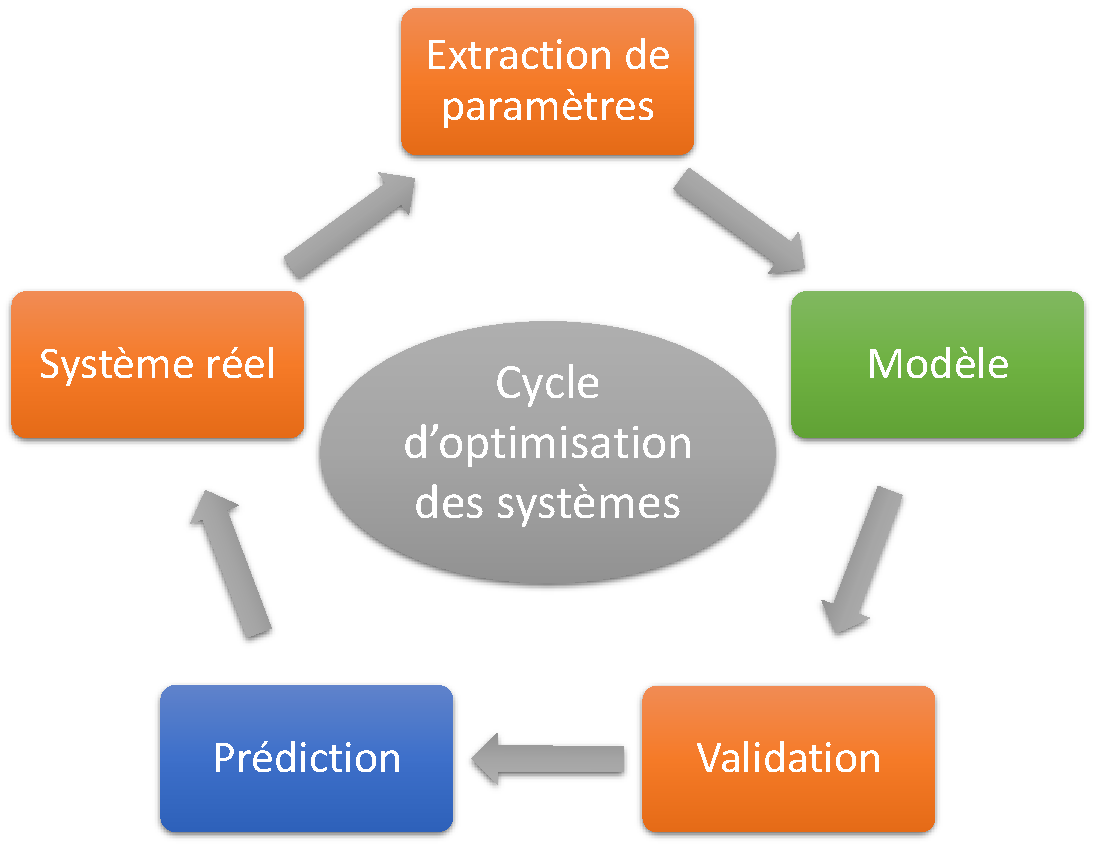
\includegraphics[scale=0.5]{chapitre3/chap3Fig/model-building.pdf}
 \caption{Le cycle d'optimisation éco-énergétique des systèmes informatiques.}
 \label{fig:model-building}
\end{figure}

La modélisation de l'énergie est un domaine de recherche actif. Il existe une panoplie des travaux dans la littérature, des revues comme \cite{Beloglazov11,Reda12,Ge13,Orgerie14,Dayarathna16} donne un aperçu global sur ces travaux sur plusieurs niveaux (architecture, système, composants, circuit, système d'exploitation, application, etc.) et avec une classification détaillée. Cependant, un modèle de coût énergétique de base peut être formuler comme suit :
\begin{equation}
 E = \alpha \; I_{cpu} + \beta \; I_{mem} + \gamma \; I_{es} + \delta \; I_{com} + \epsilon 
\end{equation} 
Où $I_{cpu}$, $I_{mem}$, $I_{es}$ et $I_{com}$ représentent le nombre d'instructions du processeur, l'utilisation de la mémoire, le débit d'E/S de disque et le nombre de transfert réseau respectivement. $\epsilon$ est une valeur d'erreur ou perturbation, qui représente les erreurs dans les mesures. Les poids $\alpha$, $\beta$, $\gamma$ et $\delta$ sont obtenus par une phase d'extraction de paramètres et l'étude du comportement des composants matériels sur la consommation d'énergie. Souvent, cette phase s'appuie sur les techniques d'apprentissage automatique \cite{Michalski13}.

% 4.2 Benchmarks: A Survey on Energy-Efficient Data Management
\subsubsection{Benchmarking}
Dans la deuxième catégorie des méthodes d’évaluation de l'énergie on trouve les benchmarks. Un indice de référence, ou benchmark, est un instrument d’analyse, de sensibilisation et de motivation des chercheurs. Il s’agit de définir des références pour se comparer aux meilleurs techniques de la branche d'EE, dans le but d’exploiter les potentiels d’amélioration en matière de gestion énergétique et de réaliser des économies \cite{Rivoire08phd}.

Les chercheurs, les agences gouvernementales et les consortiums standard de l'industrie pour les mesures de la performance, y compris \textit{Transaction Processing Performance Council} (\acrshort[hyper=false]{TPC}), \textit{Standard Performance Evaluation Corporation} (\acrshort[hyper=false]{SPEC}) et \textit{Storage Performance Council} (\acrshort[hyper=false]{SPC}) ont développé des benchmarks pour mesurer la consommation d'énergie des systèmes informatiques. Poess \textit{et al.} ont donné un aperçu très complet des benchmarks énergétiques actuellement disponibles. Il ont analysé leurs points communs et leurs différences selon diverses dimensions, y compris les composantes matérielles, la charge de requêtes et le type d'application, ainsi que les métriques et les exigences de précision et de calibration \cite{Poess10,PoessN08}.

\paragraph{TPC}
Le TPC a développé la norme \textit{TPC-Energy} \cite{Young10,TPCE} conçue pour augmenter les benchmarks de TPC existants avec des mesures d'énergie, afin que les utilisateurs finaux puissent comprendre les coûts d'énergie associés à un résultat d'un benchmark spécifique. Le nouvel benchmark répond à la demande émergente des mesures liées à l'énergie. Alors que TPC-C, TPC-E et TPC-CH ne fournissent que des mesures de performances, TPC-Energy introduit des mesures pour la consommation d'énergie pendant le traitement des requêtes. TPC-Energy régule en outre comment les mesures de puissance doivent être effectuées. Par exemple, quels sont les dispositifs de mesure à utiliser et quelle précision de mesure doit être maintenue. Les mesures définies par TPC-Energy sont la \textit{consommation d'énergie} par rapport au \textit{travail effectué} exprimée en \textit{Joule} par \textit{transaction} \cite{Schall11}.

\paragraph{SPEC}
SPEC a introduit le benchmark \textit{SPECpower\_ssj2008} \cite{SPECpowerssj2008} pour mesurer les performances et la consommation d'énergie d'un système exécutant des charges de travail basées sur Java. Le benchmark exerce les CPU, les caches, la hiérarchie de mémoire et l'évolutivité des processeurs de mémoire partagée sur plusieurs niveaux de charge. Le benchmark fonctionne sur une grande variété des systèmes d'exploitation et d'architectures matérielles avec la prise en charge des multi-nœuds. Contrairement à TPC-Energy, le benchmark SPEC mesure la consommation électrique de 0\% de charge à 100\% de charge et agrège les mesures par la moyenne géométrique pour former un seul résultat. En outre, les nouvelles versions du benchmark SPEC comme \textit{SPECweb\_2009} et \textit{SPECvirt\_sc2010} intègrent les méthodes de mesure de puissance de SPECpower.

\paragraph{SPC}
De plus, le SPC, dont les benchmarks sont focalisés sur l'évaluation des composants de stockage, a défini des extensions liées à l'énergie pour leurs benchmarks \cite{SPCBenchmark}. Ces extensions ne suivent pas la puissance maximale consommée à la charge, mais la mesurent à 80\% (notée intense) et 50\% (notée modérée) des performances maximales ainsi qu'en mode veille. En outre, ils introduisent la consommation d'énergie moyenne pondérée basée sur trois modes d'utilisation différents (faible, moyen et élevé).

\paragraph{Green500}
Le projet \textit{Green500} \cite{Green500} vise à la sensibilisation sur l'impact environnemental et à la durabilité à long terme des supercalculateurs haut de gamme en fournissant un classement des supercalculateurs les plus éco-énergétiques au monde. La liste de Green500 utilise << Performance par Watt >> comme métrique pour classer l'EE des supercalculateurs. La performance est définie comme la performance maximale obtenue, GFLOPS (Giga opération en virgule flottante par seconde), par le benchmark Linpack \footnote{\url{https://www.top500.org/project/linpack/}} sur l'ensemble du système. La puissance est définie comme la consommation d'énergie moyenne du système pendant l'exécution de Linpack.

\paragraph{JouleSort}
À part les benchmarks proposés par les organismes spécialisés, la communauté des bases de données elle-même a proposé un benchmark en matière d'énergie pour évaluer l'EE des systèmes informatiques. Le benchmark \textit{JouleSort} \cite{Rivoire07} est un benchmark de tri, dont l'idée est de mesurer l'énergie consommée pour trier une taille de données. Il mesure l'EE des systèmes à leur maximum d'utilisation (100\% de la charge). Il s'agit d'une extension du \textit{Sort Benchmark}\footnote{\url{http://sortbenchmark.org/}}, qui est utilisé pour mesurer la performance et le coût-performance des systèmes informatiques. JouleSort mesure le coût d'une certaine quantité de travail, avec une certaine mesure de consommation de puissance, par exemple : la puissance moyenne, la puissance de pic et l'énergie totale.

\subsection{Approches d'EE dans les systèmes informatiques}
Aujourd'hui, les enjeux de l'informatique éco-énergétique sont de plus en plus étudiés à tous les niveaux dans les infrastructures informatiques. Compte tenu d'une brève description des méthodes d'évaluation d'énergie dans les systèmes, nous présentons dans cette section un état de l'art des travaux d'EE des systèmes informatiques sur trois niveaux : (1) matériel, (2) système d'exploitation et (3) application. La \ref{fig:ee-it} illustre l'interdépendance des différents niveaux qui ont un impact sur la consommation d'énergie des systèmes informatiques.

\begin{figure}
 \centering
 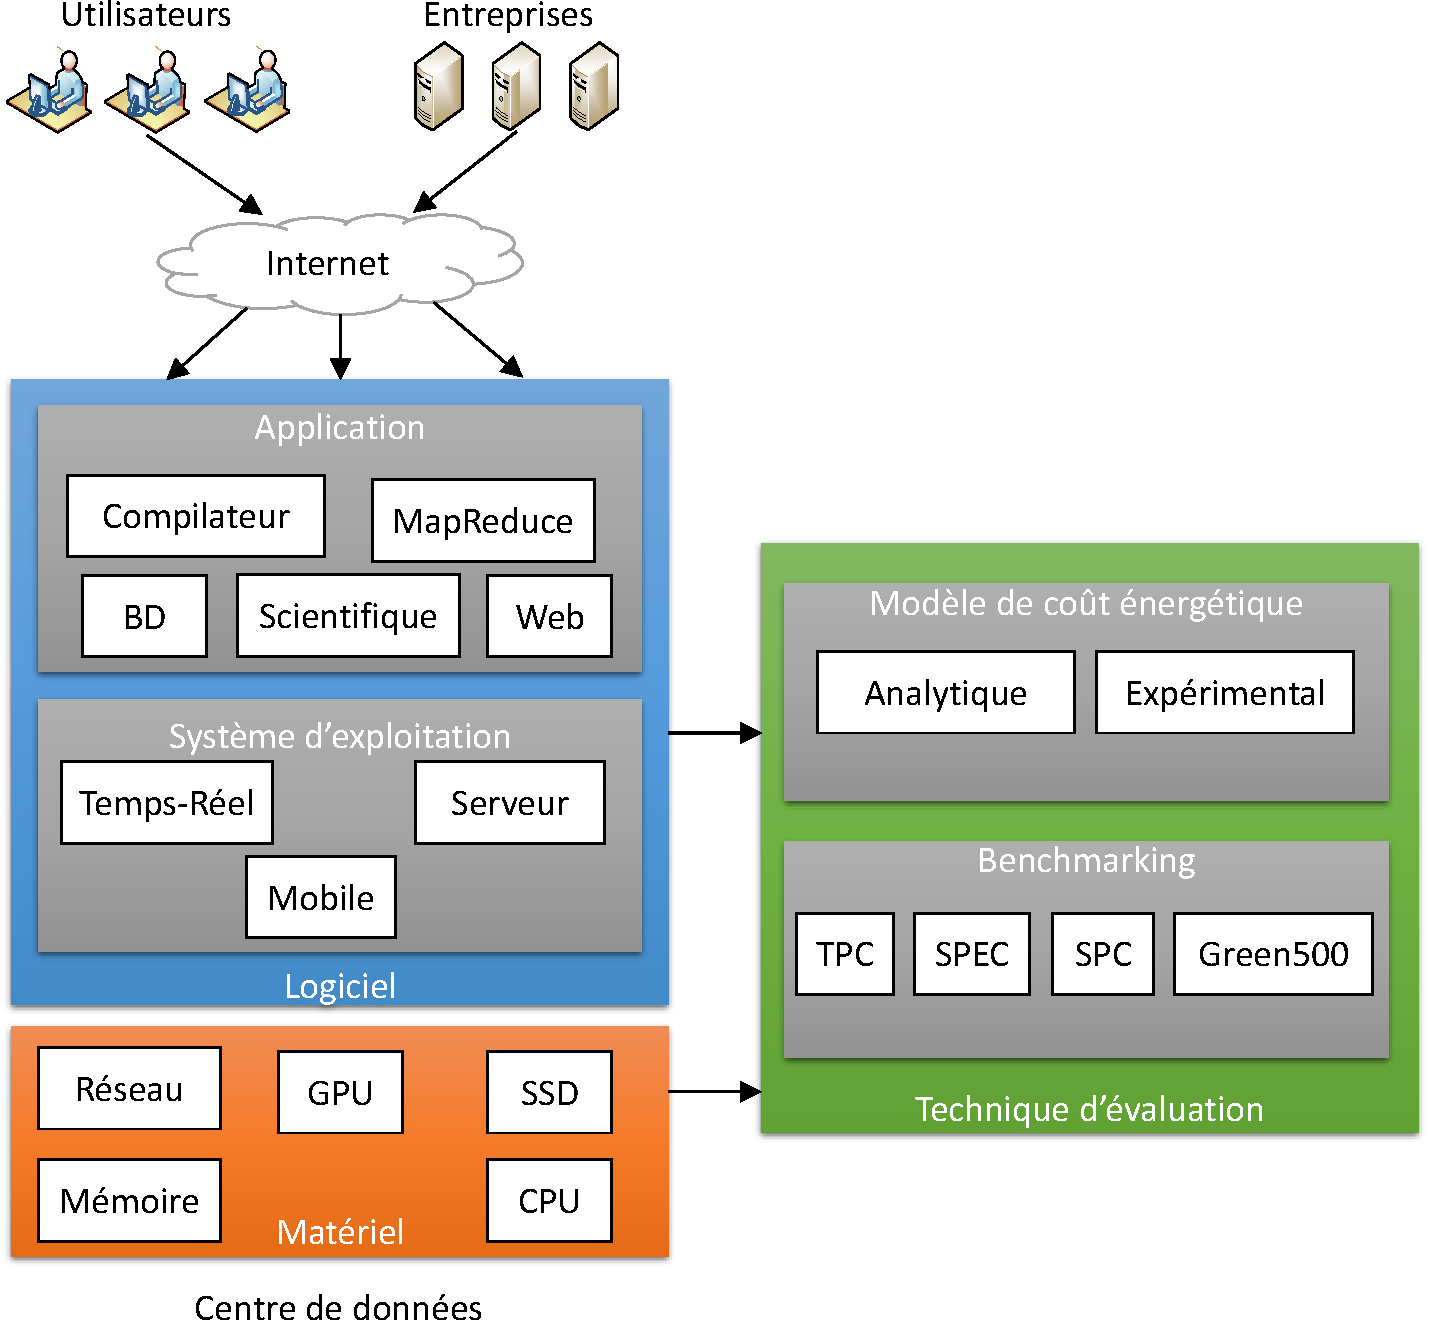
\includegraphics[scale=0.45]{chapitre3/chap3Fig/ee-it.pdf}
 \caption{La consommation d'énergie dans les systèmes informatiques sur les trois niveaux.}
 \label{fig:ee-it}
\end{figure}

\subsubsection{Approches d'EE au niveau matériel}
Un ordinateur de calcul comprend plusieurs composants, chacun pouvant être optimisé pour économiser l'énergie. Nous allons évoquer brièvement les techniques importantes proposées pour chaque composant.

Afin de réduire la consommation d'énergie du CPU, les auteurs de \cite{Weiser94} ont proposé un travail original. L'idée de base est le contrôle dynamique de la vitesse d'horloge pour réduire la consommation d'énergie pour un travail particulier. L'avantage provient de la réduction dans la tension électrique qui suit le ralentissement de l'horloge. Comme un inconvénient pour appliquer cette technique, le temps d'exécution augmente. Ce travail a largement inspiré le développement de la technique d'ajustement dynamique de la tension (DVS), et également la communauté des chercheurs. Encouragés par ces avantages, les chercheurs dans \cite{Yao95} ont construit un modèle théorique sur la base de travail précédent. L'objectif est de trouver le moyen le plus économe en énergie pour ordonnancer les tâches tout en respectant les délais d'exécution. L'ordonnancement heuristique en ligne des tâches apériodiques tout en conservant la faisabilité des ensembles de tâches périodiques est présenté dans \cite{Hong98}. Un algorithme éco-énergétique pour l'ordonnancement sans préemption est proposée dans \cite{Hong99}. Une autre méthode tente de ralentir le CPU à chaque fois qu'il y a une seule tâche éligible pour l'exécution, a été développée dans \cite{Shin99}. Une approche plus agressive est présentée dans \cite{Aydin01}, où deux algorithmes hors et en ligne sont considérés en respectant les délais, tout en réduisant la vitesse du cycle CPU autant que possible. Une comparaison systématique des différents algorithmes d'ordonnancement sur le rapport temps/performance est démontrée dans \cite{Govil95}. Dans \cite{Pillai01}, les informations de la date limite sont adoptées dans le système d'exploitation en temps réel avec la technique DVS. La norme ACPI  (\textit{Advanced Configuration and Power Interface}), disponible sur la plupart des systèmes d'exploitation, fournit une interface standard pour gérer les états de puissance du processeur \cite{Bergamaschi12}. Pour résumer, la plupart de ces algorithmes d'ordonnancement proposés tentent de tirer parti de l'EE et des contraintes temporelles d'un système en temps réel, à fin d'adapter le meilleur compromis raisonnable entre la tension électrique et les performances.

Par rapport à l'intérêt de la recherche dans l'utilisation du processeur, il y avait d'autres voix disant que le DVS peut-être également appliquée sur d'autres composantes, telle que la gestion de la mémoire. Les auteures de \cite{Fan03} illustrent par simulation que ni la gestion d'alimentation de mémoire ni encore la technique DVS sur le processeur, peuvent économiser l'énergie de façon spectaculaire. Mais en combinant les deux techniques ensemble, 89\% d'économie d'énergie, par rapport au cas de base, peut être achevé. Les techniques d'optimisation et les algorithmes proposés \cite{Lebeck00,Park11,Wu12} se sont concentrés sur les opportunités de basculer la mémoire entière ou une partie d'elle en mode faible consommation, soit pendant ou au moment de l'exécution des processus. D'autres technologies émergentes telles que la mémoire à changement de phase (PCM) \cite{Zhou09}, transfert de spin \cite{Wang08} et memristor \cite{Niu10} ont également été proposées comme des alternatives de la mémoire principale économe en énergie.

Les unités de traitement graphique (\acrshortpl[hyper=false]{GPU}) sont également devenues une partie essentielle des centres de données hébergeant des applications scientifiques à cause de leur efficacité dans les fonctions à virgule flottante. De plus, les GPUs sont très efficaces sur le plan énergétique par rapport aux processeurs. Les deux principales machines supercalculateur à haut rendement énergétique sont basées sur GPU \cite{Green500}. Les GPUs fournissent près de 85 fois moins de consommation d'énergie pour un calcul en virgule flottante que les processeurs x86 \cite{Keckler11}.

Il existe deux techniques de base pour atteindre l'EE dans les équipements de stockage : (1) rendre le matériel de stockage économes en énergie, et (2) réduire la redondance des données \cite{Yoder10}. Le principal objectif du matériel de stockage éco-énergétique est constitué par les disques SSDs (Solid-State Drive). Les disques SSD utilisent une mémoire Flash, c'est-à-dire une mémoire non volatile ayant des caractéristiques similaires à la mémoire morte effaçable électriquement et programmable (EEPROM). Les SSDs ont des propriétés proportionnelles à l'énergie, du fait que l'énergie utilisée est proportionnelle aux opérations d'E/S par seconde \cite{Shuja16}. D'autre part, les disques durs (HDDs) consomment 85\% d'énergie lorsqu'ils sont inactifs \cite{Narayanan09}. Les SSDs deviennent l'avenir du stockage primaire économe en énergie dans les systèmes.

Les périphériques réseau constituent une autre ressource énergétique dans les centres de données \cite{Orgerie14}. La consommation d'énergie dans les périphériques réseau peut être gérée par des techniques de taux de liaison adaptatif (ALR) \cite{Bilal13,Bilal14}. Les techniques d'ALR atteignent l'EE par : (1) des débits de données réduits, ou (2) des transitions d'état de puissance inférieure/inactive qui sont gérées en fonction des charges de données \cite{Bilal13b}. Les protocoles de routage efficaces jouent un rôle important dans l'utilisation de la capacité réseau. Shang \textit{et al.} \cite{Shang10} ont avancé l'idée du routage énergétique où peu de périphériques réseau fournissent le routage de base et le débit en fonction d'un seuil de performance tandis que le reste des périphériques sont hors tension.

\subsubsection{Approches d'EE au niveau système d'exploitation}
La communauté de la recherche a rapidement réalisé l'impact significatif de la couche système sur la consommation d'énergie. Le travail de \cite{Benini00} classe les composants du système consommant la majeure partie de l'énergie en trois catégories : unités de calcul, unités de communication et unités de stockage. Les auteurs présentent également un état de l'art des techniques éco-énergétique autour de trois phases principales d'une conception de système : la conceptualisation et la modélisation, la conception et la mise en œuvre, et la gestion d'exécution. Les recherches montrent ainsi que les systèmes d'exploitation (SE) ont une consommation d'énergie hétérogène et peuvent-être optimisés pour consommer moins d'énergie. La consommation varie même entre les versions du même SE. Par exemple, la consommation d'un ordinateur sous différentes versions de Windows et des noyaux Linux, suivent des méthodologies de mesures similaires, présente des variations non négligeables \cite{Orgerie14}. Les auteurs de \cite{Pallipadi06} ont développé un gestionnaire d'alimentation en temps réel dans le noyau pour le système d'exploitation Linux appelé le gouverneur à la demande (LGD). Le gestionnaire surveille en permanence l'utilisation du processeur et définit une fréquence d'horloge qui correspond aux exigences de performances actuelles, ce qui minimise la consommation d'énergie. Le travail de \cite{Zeng02} a proposé et développé \textit{ECOsystem}, un framework pour la gestion de l'énergie en tant que ressource de première classe dans un SE destinée aux dispositifs alimentés à l'aide de batterie tels que les mobiles. ECOsystem fournit une interface pour définir une durée de vie de la batterie cible et des priorités d'application utilisées pour déterminer la quantité d'énergie qui sera allouée aux applications à chaque période. Des techniques similaires ont été proposées pour les mobiles comme : \textit{Nemesis OS} \cite{Neugebauer01}, \textit{GRACE} \cite{Sachs04,Vardhan09} et \textit{Coda/Odyssey} \cite{Flinn04}, et pour les serveurs : \textit{Linux/RK} \cite{Rajkumar97}, \textit{PowerNap} \cite{Meisner09} et \textit{Barely Alive} \cite{Anagnostopoulou12}.

\subsubsection{Approches d'EE au niveau application}
L'EE au niveau application est devenu un domaine de recherche actif pour les raisons suivantes : (1) les techniques d'optimisation de bas niveau (matériel et SE) dépend fortement de l'estimation précise des profils de puissance des applications. Cependant, beaucoup d'informations et de statistiques nécessaires pour ces estimations ne sont disponibles que dans le niveau application. (2) De nombreuses applications peuvent être exécutées de différentes manières pour accomplir la même tâche de calcul. Les applications éco-énergétique, qui adaptent leurs comportements en fonction des états liés à l'alimentation des systèmes sous-jacents, peuvent offrir des possibilités supplémentaires d'économie d'énergie. De nombreux projets de recherche dans ce domaine sont consacrés aux services Web \cite{Bohrer02,Sharma03,Chase01,Chen05}, les compilateurs \cite{Hsu03,Huang07,Kadayif05} et les environnements de développement (EDI) \cite{Capra12}. Dans \cite{Xian07}, un framework de programmation à usage général a été développé pour permettre aux applications d'être exécutées avec des plans différents en fonction de leurs coûts d'énergie. \textit{SEEDS} est un framework pour aider les ingénieurs des logiciels à développer des applications éco-énergétiques de haut niveau \cite{Manotas14}. SEEDS fournit une analyse automatisée, une prise de décision et une mise en œuvre visant à optimiser la consommation d'énergie d'une application donnée. Une application récente des techniques éco-énergétique inclut \textit{MapReduce} \cite{Chen12,Lang10,Leverich10}.

Et encore plus récemment, la consommation d'énergie dans les bases de données commence à attirer l'attention de la communauté des chercheurs. L'objectif principal de ces efforts est de concevoir des SGBDs avec la consommation optimisée d'énergie. Notre étude s'inscrit dans cette catégorie, et nous allons détailler dans une section séparée les différents travaux de littérature sur l'EE dans les bases de données. La \ref{fig:energy-approaches-classification} représente une classification des travaux d'EE dans les systèmes informatiques sur les trois niveaux discutés.

\begin{figure}
\footnotesize
\begin{center}
\tikzset{
  basic/.style  = {draw, text width=4cm, drop shadow, rectangle},
  root/.style   = {basic, rounded corners=2pt, thin, align=center,
                   fill=green!30},
  level 2/.style = {basic, rounded corners=6pt, thin,align=center, fill=green!60,
                   text width=8em},
  level 3/.style = {basic, thin, align=left, fill=pink!60, text width=8.5em}
}
\begin{tikzpicture}[
  level 1/.style={sibling distance=50mm},
  edge from parent/.style={->,draw},
  >=latex]

% root of the the initial tree, level 1
\node[root] {Approches d'EE dans les systèmes informatiques}
% The first level, as children of the initial tree
  child {node[level 2] (c1) {Niveau matériels}}
  child {node[level 2] (c2) {Niveau SE}}
  child {node[level 2] (c3) {Niveau application}};

% The second level, relatively positioned nodes
\begin{scope}[every node/.style={level 3}]
\node [below of = c1, xshift=15pt] (c11) {CPU \cite{Weiser94,Yao95,Hong98,Hong99,Shin99,Aydin01,Pillai01,Bergamaschi12}};
\node [below of = c11] (c12) {Mémoire \cite{Fan03,Lebeck00,Park11,Wu12,Zhou09,Wang08,Niu10}};
\node [below of = c12] (c13) {GPU \cite{Keckler11,Green500}};
\node [below of = c13] (c14) {Stockage \cite{Yoder10,Shuja16,Narayanan09}};
\node [below of = c14] (c15) {Réseau \cite{Orgerie14,Bilal13,Bilal14,Bilal13b,Shang10}};

\node [below of = c2, xshift=15pt] (c21) {LGD \cite{Pallipadi06}};
\node [below of = c21] (c22) {Mobiles \cite{Zeng02,Neugebauer01,Sachs04,Vardhan09,Flinn04}};
\node [below of = c22] (c23) {Serveurs \cite{Rajkumar97,Meisner09,Anagnostopoulou12}};

\node [below of = c3, xshift=15pt] (c31) {Services Web \cite{Bohrer02,Sharma03,Chase01,Chen05}};
\node [below of = c31] (c32) {Compilateurs \cite{Hsu03,Huang07,Kadayif05}};
\node [below of = c32] (c33) {EDI \cite{Capra12,Manotas14}};
\node [below of = c33] (c34) {MapReduce \cite{Chen12,Lang10,Leverich10}};
\node [below of = c34] (c35) {Base de données};
\end{scope}

% lines from each level 1 node to every one of its "children"
\foreach \value in {1,...,5}
  \draw[->] (c1.178) |- (c1\value.west);

\foreach \value in {1,...,3}
  \draw[->] (c2.178) |- (c2\value.west);
  
\foreach \value in {1,...,5}
  \draw[->] (c3.178) |- (c3\value.west);
\end{tikzpicture}
\caption{Classification des approches d’EE dans les systèmes informatiques.}
\label{fig:energy-approaches-classification}
\end{center}
\end{figure}

\section{Approches d'EE dans les BD}
%La gestion de l'énergie des systèmes de bases de données est devenue un sujet de recherche important au cours des dernières années. Les travaux de recherche proposés comprennent à la fois les dimensions matérielles et logicielles.
%Deux hypothèses principales ont été retenues pour ces initiatives: (i) applications de base de données déjà déployées ($\mathcal{BDDD}$) et (ii) applications de base de données non déployées ($\mathcal{BDND}$). Dans la première hypothèse, nous considérons que l'application de base de données est déjà conçue et déployée sur une plate-forme donnée. En ce qui concerne les initiatives avec l'hypothèse de $\mathcal{BDND}$, la majorité des études couvrent la partie matériel. Dans cet thèse, nous nous concentrons uniquement sur une initiative concernant les techniques logicielles avec l'hypothèse $\mathcal{BDDD}$.

La gestion de l'énergie des systèmes de bases de données est devenue un sujet de recherche important au cours des dernières années. Il y a eu une pléthore d'études et d'initiatives de la communauté des chercheurs. Lors de l'étude de la littérature des travaux, on distingue principalement deux approches principales : \textit{Approches Orientées Matériels} ($\mathcal{\acrshort[hyper=false]{AOM}}$) et \textit{Approches Orientées Logicielles} ($\mathcal{\acrshort[hyper=false]{AOL}}$). Dans les sections suivantes, nous détaillons les travaux de chaque approche.
%comme le montre la Figure . %Dans cette section, nous proposons une enquête et une classification de ces approches, comme le montre la \ref{fig:energy-approaches-classification}.

\subsection{$\mathcal{AOM}$}
Les approches matérielles utilisent des solutions << naïves >> comme la désactivation de composants électroniques pendant les périodes d'inactivité, et des solutions avancées telles que la modification dynamique de la performance des composants matériels pour une meilleure EE, qui peut être illustrer par la technique DVFS offerte par les CPU d'aujourd'hui \cite{Beloglazov11}. Par ailleurs, les techniques appliquées au niveau du matériel peuvent être divisées en deux catégories: (i) dispositif de traitement et (ii) la gestion du stockage.

\subsubsection{Dispositif de traitement}
Les techniques appartenant à cette catégorie utilisent de nouvelles approches pour minimiser la consommation d'énergie des appareils informatiques.
Lang \textit{et al.} ont proposé le mécanisme PVC (Processor Voltage/Frequency Control) pour équilibrer la consommation d'énergie et la performance \cite{Lang09}. Il vise à exécuter des instructions à une tension et une fréquence de processeur basse en tirant parti de la capacité des processeurs modernes. Une technique similaire est utilisée dans \cite{Tu14}, les auteurs rapportent 51,3\% des économies d'énergie. La technique proposée ajuste dynamiquement le niveau DVFS du processeur en fonction des performances du SGBD ou le plan de requête choisi pour l'exécution. Xu \textit{et al.} \cite{Xu13b} aussi utilisent la technique DVFS avec un mécanisme de contrôle de rétroaction pour les charges de requêtes d'une base de données. Afin d'économiser l'énergie, ils gèrent le niveau DVFS en fonction du débit de travail (\textit{throughput}) et des caractéristiques de la charge de requêtes (par exemple, en basant sur le nombre d'E/S ou de CPU). Dans une autre étude, une co-ingénierie entre Oracle et Intel tente de réduire les coûts d'exploitation et de répondre efficacement aux objectifs d'informatique durable (\textit{green computing}) a donné lieu à une nouvelle version de \textit{Oracle Exadata Database Machine} \cite{IntelOracle14}. La solution proposée met dynamiquement le processeur Intel Xeon et la mémoire dans l'état de puissance disponible le plus bas convenable pour répondre aux exigences de la charge de requêtes. Cependant, les techniques mentionnées ci-dessus souffrent des frais additionnels pour la transition vers des états de faible puissance, qui conduisent généralement à une consommation d'énergie supplémentaire et des délais d'exécution causés par la réinitialisation des composants \cite{Beloglazov11}.

Pour accélérer les applications de données intensives, les Field-Programmable Gate Array (FPGA) sont utilisés à la place des processeurs classiques, principalement parce qu'ils permettent la construction de matériel personnalisé à des coûts de développement relativement faibles. De plus, il a déjà été montré dans \cite{Woods14} que les solutions à base de FPGA ont le potentiel d'améliorer la performance et en même temps de réduire la consommation d'énergie. Les auteurs rapportent que l'utilisation de ces propositions pour certaines requêtes, permet au système de consommer que 216 \textit{Joules}, alors que les techniques traditionnelles consomment 3888 \textit{Joules}.

Les unités de traitement graphique (GPU) ont été considérées comme une excellente alternative aux processeurs pour leur haute performance, leur haut débit de traitement ainsi que leur économie d'énergie. Une étude a rapporté que l'utilisation d'un GPU est plus économe en énergie lorsque l'amélioration de la performance est supérieure à une certaine borne, par rapport à une solution CPU classique \cite{Rofouei08}. Le CPU-GPU co-traitement est une autre tendance intéressante dans la technologie de base de données, qui consiste à exploiter les avancées matérielles ainsi que la conception d'algorithmes optimisés pour améliorer les performances de traitement des requêtes et l'EE. Les résultats de comparaison entre une architecture CPU-GPU discrète et une architecture CPU-GPU couplée montrent que la consommation moyenne d'énergie de l'architecture discrète est entre 36\% et 44\% supérieurs à celle de l'architecture couplée \cite{Hurson16}.

D'autre part, des études récentes telles que \cite{Do13} affirment que l'utilisation de disques Smart Solid State (SSSDs) pour traiter les données peuvent-être plus avantageux à la fois en terme de performance et de consommation d'énergie. Les SSSDs se sont des dispositifs de stockage flash qui intègrent une mémoire et un processeur à l'intérieur du dispositif de SSD, et pourrait être utilisé pour exécuter des programmes généraux définis par l'utilisateur. Les auteurs de \cite{Do13} améliorent l'EE du traitement des requêtes en réduisant son temps d'exécution et/ou en exécutant le traitement sur le processeur de faible puissance qui vient avec les SSSDs. Les premiers résultats de l'exécution d'un sous-ensemble de requêtes SQL (simples requêtes de sélection et d'agrégation) sur un SSSD fournissent jusqu'à 3x de réduction de la consommation d'énergie. Les SSSD ont beaucoup de potentiel, mais les capacités de calcul des appareils embarqués dans les SSSD actuels sont trop limitées pour gérer le volume de données énormes.

\subsubsection{Gestion du stockage}
Les dispositifs de traitement ont été considérés comme les principaux contributeurs à la consommation d'énergie dans un serveur. Cela dit, la consommation d'énergie des dispositifs de stockage secondaire et de la mémoire ont également attiré une forte attention des chercheurs en raison de leurs capacités de croissance significative au cours des dernières années.
Les approches de gestion de stockage tentent de trouver un bon niveau de consolidation de la charge, l'amélioration des techniques de mise en cache et de préchargement et l'optimisation des modes d'alimentation dans les matrices de disques afin de minimiser la dissipation d'énergie \cite{Tu14}. Dans \cite{Harizopoulos09}, les auteurs fournissent des expériences pour montrer que les choix effectués par les systèmes de base de données peuvent améliorer l'EE. Plus précisément, repartitionner la base de données sur 66 disques propose une augmentation de 14\% de l'efficacité contre la dégradation de 45\% de la performance. Les auteurs de \cite{Tu14} ont proposé un modèle d'optimisation intégrée pour la migration des données et l'ajustement de l'état du disque, dans lequel ils placent dynamiquement les enregistrements dans un fragment selon la fréquence des enregistrements de données d'accès. Les résultats présentés montrent que près de 50\% de l'énergie peut être économisé en utilisant les techniques proposées. Dans la même direction, le travail de \cite{Behzadnia16} propose un modèle de gestion de puissance dynamique qui prend des décisions en temps réel sur le passage des disques à des modes de faible puissance. Le modèle est intégré dans le SGBD et utilisé pour obtenir le compromis optimal entre la consommation d'énergie et le temps de réponse des requêtes. Le rapport montre 60\% des économies d'énergie.

L'utilisation de disques SSD comme un périphérique de stockage des bases de données pour améliorer l'EE est une autre direction qui a été étudiée par des travaux récents. Dans \cite{Schall10}, les auteurs ont étudié le comportement de la performance et la consommation d'énergie des SSD pour des schémas d'accès typiques pour les applications de base de données à forte intensité d'E/S. Ils montrent, en outre, que la technologie SSD offre un nouveau niveau de performance et d'EE, et suggèrent l'exploitation de leurs nouvelles caractéristiques par les serveurs de base de données. De même, le travail de \cite {Cheong12} analyse et évalue les performances de traitement des données et l'EE des SSD et système de stockage. Comme son prédécesseur, les auteurs montrent l'amélioration de la performance et l'EE.

\begin{figure}
\footnotesize
\begin{center}
\tikzset{
  basic/.style  = {draw, text width=4cm, drop shadow, rectangle},
  root/.style   = {basic, rounded corners=2pt, thin, align=center,
                   fill=green!30},
  level 2/.style = {basic, rounded corners=6pt, thin,align=center, fill=green!60,
                   text width=8em},
  level 3/.style = {basic, thin, align=left, fill=pink!60, text width=8.5em}
}
\begin{tikzpicture}[
  level 1/.style={sibling distance=50mm},
  edge from parent/.style={->,draw},
  >=latex]

% root of the the initial tree, level 1
\node[root] {Approches orientées matériels}
% The first level, as children of the initial tree
  child {node[level 2] (c1) {Dispositif de traitement}}
  child {node[level 2] (c2) {Gestion du stockage}};

% The second level, relatively positioned nodes
\begin{scope}[every node/.style={level 3}]
\node [below of = c1, xshift=15pt] (c11) {CPU \cite{Lang09,Tu14,Xu13b,IntelOracle14,Beloglazov11}};
\node [below of = c11] (c12) {GPU \cite{Rofouei08}};
\node [below of = c12] (c13) {FPGA \cite{Woods14}};
\node [below of = c13] (c14) {Co-Traitement \cite{Hurson16,Do13}};

\node [below of = c2, xshift=15pt] (c21) {HDD \cite{Tu14,Harizopoulos09,Behzadnia16}};
\node [below of = c21] (c22) {SSD \cite{Schall10,Cheong12}};
\node [below of = c22] (c23) {Mémoire \cite{Appuswamy15,Korkmaz15,Xu10b}};
\end{scope}

% lines from each level 1 node to every one of its "children"
\foreach \value in {1,...,4}
  \draw[->] (c1.178) |- (c1\value.west);

\foreach \value in {1,...,3}
  \draw[->] (c2.178) |- (c2\value.west);
\end{tikzpicture}
\caption{Classification des approches d’EE orientées matériels.}
\label{fig:hardware-approaches-classification}
\end{center}
\end{figure}

La mémoire est un autre consommateur d'énergie important dans les systèmes informatiques, en particulier avec l'utilisation croissante des bases de données orientée colonnes où le stockage des données se fait directement dans la mémoire. De nombreux travaux de recherche récents commencent à étudier l'impact du dispositif de mémoire sur la consommation d'énergie. L'enquête faite dans \cite{Appuswamy15} souligne que l'utilisation croissante des bases de données en mémoire va bientôt émerger la mémoire en tant que consommateur de puissance électrique dominante au lieu de CPU. Comme pour les composants précédents, la mémoire principale a également des différents états de puissance et de la fréquence à modifier en fonction de son utilisation. Sur cette base, les auteurs ont utilisé la fréquence mise à l'échelle et des modes de mise hors tension des DRAM pour améliorer la consommation d'énergie sans sacrifier les performances. Dans \cite{Korkmaz15}, les auteurs rapportent un résultat préliminaire sur une technique d'allocation de mémoire basée sur les rangs pour économiser l'énergie des systèmes de base de données. La technique permet au SGBD de déplacer les rangs inutiles de la mémoire aux états de faible puissance et réduire ainsi la consommation d'énergie globale. L'évaluation indique que la méthode proposée atteint 40\% de diminution de la puissance lorsque la taille de la base de données est plus petite que la quantité de la mémoire déjà provisionnée sur le serveur. Le travail de \cite{Hassan15} propose une architecture de mémoire hybride comprenant à la fois Dynamic Random Access Memory (DRAM) et de la mémoire non volatile (NVM) pour réduire la consommation d'énergie de base de données, grâce à une politique de gestion des données au niveau de l'application qui décide de placer des données sur la DRAM ou la NVM. Ils analysent d'abord l'exécution d'applications et de collectent des statistiques d'accès mémoire pour des objets individuels. Ceux-ci sont évalués en utilisant un modèle d'analyse de la performance et de l'énergie pour identifier la technologie de mémoire la plus adaptée pour stocker ces données. Les résultats présentés indiquent que l'utilisation de la mémoire hybride peut réduire l'énergie du système de mémoire d'environ 80\%.

\subsection{Bilan et discussion}\label{sec:bilanAOM}
Dans les sections précédentes, nous avons classé les techniques appliquées au niveau du matériel en deux catégories, dispositif de traitement et la gestion du stockage. Les études précitées dans pour chaque catégorie ont en effet apporté une contribution importante à la conservation de l'énergie (voir \ref{fig:hardware-approaches-classification}). Cependant, les $\mathcal{AOM}$ ne sont pas simple à appliquer et ont plusieurs inconvénients en particulier dans le domaine des bases de données. Tout d'abord, ils ont besoin d'utiliser du nouveau matériel, puisque les nouvelles technologies tels que DVFS ne sont pas disponibles sur tous les processeurs ou mémoires actuels. Deuxièmement, les SSD émergents sont très chers et ont un problème de durée de vie. Dernier point, mais non des moindres, il existe différentes marques/versions pour chaque composant matériel, ce qui rend ces méthodes peu pratiques en raison de leurs problèmes de portabilité.
Par conséquent, les $\mathcal{AOL}$ sont beaucoup préférés dans le cadre des bases de données, car ils sont indépendants du matériel sous-jacent. En outre, le SGBD a une connaissance détaillée des éléments internes du système, tels que la charge de requêtes, les plans d'exécution, les statistiques de base de données, etc. \cite{Korkmaz15}. Dans \cite{Harizopoulos09}, Harizopoulos \textit{et al.} de laboratoire de HP confirment que << les approches matérielles ne sont qu'une partie de la solution, et les approches logicielles seront la clé dans l'optimisation de l'efficacité énergétique >>.

\subsection{$\mathcal{AOL}$}
Les approches matérielles ne sont qu'une partie de la solution pour réduire les valeurs de puissance; les approches logicielles sont l'autre élément clé dans les mécanismes d'optimisation de l'EE. A ce niveau, les papiers de vision sur l'énergie \cite{Graefe08, Harizopoulos09} recommandent de revoir les techniques d'optimisation des requêtes, les algorithmes d’ordonnancement, la conception physique et les techniques de mise à jour de base de données en tenant compte de l'énergie. La plupart des importantes études concernent deux aspects principaux : (i) la définition des modèles de coûts pour prédire l'énergie et (ii) la proposition des techniques basées sur les modèles de coûts pour réduire l'énergie. Cette situation est tout à fait semblable à celle vécue dans les approches de conception traditionnelles axées sur l'amélioration de la performance, où la plupart des optimiseurs de requêtes des SGBD open source \footnote{\url{http://www.postgresql.org/docs/current/static/planner-optimizer.html}} et commerciale \footnote{\url{http://docs.oracle.com/cd/B10500_01/server.920/a96533/optimops.htm\#51003}} utilisent des approches fondées sur les modèles de coûts. Dans ces approches, un optimiseur basé sur les coûts estime le coût de chaque plan d'exécution possible en appliquant des formules heuristiques utilisant un ensemble de statistiques relatives à la base de données (taille des tables, des indexes, longueur de tuples, les facteurs de sélectivité de jointure et prédicats de sélection, la taille des résultats intermédiaires, etc.) et au matériel (taille du tampon mémoire, la taille de page, etc.).

\subsubsection{Définition des modèles de coûts}
Dans \cite{Xu13, Xu10b}, les auteurs proposent une extension du modèle de coût de PostgreSQL pour prédire la consommation d'énergie d'une seule requête exécutée d'une façon isolée (pas de parallélisme inter-requêtes). Un profil de puissance statique pour chaque opération de base de données basique est défini dans la phase du traitement des requêtes. Le coût de l'énergie d'un plan peut être calculé à partir des opérations de base de données SQL, comme le coût de la puissance du processeur pour accéder à un tuple, coût du disque pour la lecture/écriture d'une page et ainsi de suite, et par l'intermédiaire de différentes méthodes d'accès et d'opérations de jointure, en utilisant une technique de régression linéaire simple. La formule générale pour calculer l'énergie d'un opérateur $x$ est :
\begin{equation}
\hat{E}_x = W_{cpu} \times N_{tuples}^{m} \times N_{tuples} + \bar{W}_{E/S} \times N_{pages}
\end{equation}
Où $W_{cpu}$ et $\bar{W}_{E/S}$ sont le coefficient de consommation d'énergie d'un tuple traité par le CPU ($N_{tuples}$), et le coefficient statique d'une page traitée en E/S ($N_{pages}$), et $m$ est un coefficient de modèle pour la consommation d'énergie du CPU ($m = 0,5$ après la régression).
Les auteurs adaptent leur modèle statique pour des charges de requêtes dynamiques à l'aide d'un mécanisme de contrôle de rétroaction pour mettre à jour périodiquement les paramètres du modèle à travers des mesures d'énergie en temps réel.

Dans \cite{Kunjir12}, une recherche profonde dans la modélisation de la puissance de pic des opérations de requête est donnée. Un modèle de plans d'exécution sur la base de pipeline a été développé pour identifier les sources de consommation d'énergie de pic pour une requête isolée et de recommander des plans avec une faible puissance de pic. Pour chacun de ces pipelines, une fonction mathématique est appliquée, qui prend en entrée les taux et les tailles des données circulant à travers les opérations de pipelines. En tant que sortie, une estimation de la consommation d'énergie de pic est donné. Les auteurs ont utilisé la technique de régression multiple affine par morceaux pour construire leurs modèles de coût. Pour un nœud de base $B$ (par exemple : un accès séquentiel), le débit est calculé comme :
\begin{equation}
 Taux_B = \frac{Entrée_B}{TempsDisque_B}
\end{equation}
Où $Entrée_B$ indique la taille des données extraites du disque par $B$ et $TempsDisque$ est le temps de transfert du disque.
\begin{alignat}{2}
& \text{soit}  \quad && Base_N = SousArbre^{PL}_{N} \cap Base^{PL} \nonumber \\
& \text{alors} \quad && Taux_N = \frac{\sum_{i \in Source^{PL}_{N}} Sortie_i}{max_{x \in Base_N} TempsDisque_x}
\end{alignat}
$N$ est un nœud générique en aval dans le pipeline, $SousArbre^{PL}_{N}$ est le sous-arbre du pipeline $PL$ avec la rince $N$, $Base^{PL}$ est l'ensemble des nœuds de bases dans le pipeline $PL$, $Source^{PL}_{N}$ est l'ensemble des nœuds dans le pipeline $PL$ qui fournissent directement des entrées au nœud $N$, et $Sortie_i$ désigne la taille de la donnée en sortie par le nœud $i$. Les tailles des données sont estimées à partir de catalogue de la base de données.

Dans le même sens, le travail de \cite{Lang11} propose un framework pour un traitement éco-énergétique des requêtes dans les bases de données. Il étend les plans de requêtes produites par l'optimiseur de requête traditionnelle avec une prédiction de la consommation d'énergie pour certains opérateurs de bases de données spécifiques comme la sélection, projection et la jointure en utilisant la technique de régression linéaire. L'\ref{eq:lang11} montre le modèle le plus précis proposé pour estimer la puissance moyenne du système pendant l'exécution d'une requête isolée. Le modèle est défini par trois types de variables :
\begin{enumerate}
 \item Temps $T$
 \item Paramètres de requête $Q$ : nombre d'instructions de processeur ($I_Q$), lecture de page disque ($R_Q$), écriture de page disque ($W_Q$) et nombre d'accès au mémoire ($M_Q$)
 \item Paramètres du système : CPU ($C_{cpu}$), lecture disque ($C_R$), écriture disque ($C_W$), accès mémoire ($C_{mm}$), reste du système ($C_{autres}$). Ces paramètres quantifient la puissance des composants matériels et sont obtenus par une régression.
\end{enumerate}

\begin{equation}\label{eq:lang11}
 P_{moy} = C_{cpu} \times \frac{I_Q}{T} + C_R \times \frac{R_Q}{T} + C_W \times \frac{W_Q}{T} + C_{mm} \times \frac{M_Q}{T} + C_{autres}
\end{equation}

L'intuition derrière ce modèle est de calculer la sommation de la puissance moyenne du processeur ($C_{cpu} \times \frac{I_Q}{T}$), du lecture disque ($C_R \times \frac{R_Q}{T}$), d'écriture disque ($C_W \times \frac{W_Q}{T}$), du mémoire ($C_{mm} \times \frac{M_Q}{T}$) et du reste du système ($C_{autres}$) pendant l'exécution de la requête $Q$.

L'étude de \cite{Rodriguez11} tente de modéliser l'énergie et la puissance de pic des requêtes de sélection simples sur les relations individuelles en utilisant une régression linéaire. Le modèle développé pour la consommation d'énergie d'une requête $Q$ avec une relation $R$ est le suivant :
\begin{equation}
 E_Q = \beta_0 + \beta_1 \; S + \beta_2 \; SF_p(R) \; S + \beta_3 \; |R| \; SF_p(R) + \beta_4 \; |R| <R> SF_p(R)
\end{equation}

Où $\beta_i$ sont des coefficients de régression et $|R|$, $<R>$, $SF_p(R)$ et $S$ sont respectivement : la cardinalité de la relation $R$, le nombre de colonnes de $R$, la sélectivité du prédicat $p$ dans $R$ et le nombre de serveurs utilisés. Les requêtes sont supposées exécuter d'une façon isolée.

Alors que les travaux cités considèrent seulement une architecture de base de données centralisée, l'étude de Lang \textit{et al.} \cite{Lang12} a proposé un modèle de coût pour une architecture de base de données en grappe de serveurs. Le modèle prend en compte les configurations de serveur (par exemple, le CPU, les disques et la bande passante du réseau) et les paramètres de traitement de données (par exemple, la sélectivité des prédicats, la taille de la table de hachage), et prédit les performances de traitement des données et l'EE pour un opérateur de jointure par hachage. L'erreur maximale rapportée est inférieure à 10\%.

\subsubsection{Techniques basées sur des modèles de coûts}
Les modèles de coûts proposés pour prédire l'énergie sont ensuite utilisés dans diverses techniques pour optimiser la consommation d'énergie de base de données. Les auteurs de \cite{Lang09} ont proposé un mécanisme pour améliorer l'EE des requêtes en introduisant des retards explicites, en utilisant l'agrégation des requêtes pour tirer parti des composants de requêtes communs dans la charge. Le retard explicite permet de grouper les requêtes dans une file d'attente en mémoire tampon, ce qui conduit alors à une évaluation plus efficace de l'ensemble du lot par des techniques d'optimisation multi-requêtes. Pour la comparaison de l'énergie et du temps, la métrique utilisée est le Produit Énergétique/Délai (\acrshort[hyper=false]{EDP}) \cite{Laros13}, qui est le produit de l'énergie et du délai : 
\begin{equation}\label{eq:edp}
 EDP = \text{énergie} (Joules) \times \text{temps} (sec)
\end{equation}
Après la substitution, la formule finale de comparaison est :
\begin{equation}
 EDP = V^2 / F
\end{equation}
Où $V$ est le voltage et $F$ est la fréquence du processeur. Les résultats d'expérimentations pour les requêtes de sélection simples montrent que cette technique peut être utilisé pour trouver un compromis entre la performance et l'énergie, ce qui réduit la consommation d'énergie de 54\% contre 43\% d'augmentation dans le temps de réponse moyen.

Le travail de \cite{Psaroudakis14} indique que l'ordonnancement éco-énergétique de plusieurs requêtes peut améliorer l'EE de certains opérateurs SQL basique qui peuvent être exécutées en parallèles, tels que les agrégations et les algorithmes d'accès aux données. La métrique utilisée pour choisir le meilleur compromis entre le temps et l'énergie est EDP (\ref{eq:edp}). Les résultats expérimentaux montrent que l'application des méthodes proposées, l'EE est augmenté jusqu'à 4x. Dans le même sens, les auteurs de \cite{Kang08} proposent un système de gestion de la mémoire cache éco-énergétique pour les bases de données en temps réel sur la mémoire flash. La technique introduite crée une partition logique du pool global de la mémoire tampon dans des pools de mémoire tampon de lecture et d'écriture, et le contrôle de rétroaction dynamique ajuste la taille des pools pour satisfaire les objectifs de performance et de consommation d'énergie.

Le travail de \cite{Lang11} a montré que le traitement d'une requête aussi vite que possible ne s'avère pas toujours être la façon la plus économe en énergie dans un SGBD. Sur la base de leurs modèles de coût proposé pour prédire l'énergie, ils choisissent des plans de requêtes qui réduisent la consommation d'énergie et répondent aux objectifs de performance traditionnels. Ce choix est fait manuellement. Les résultats montrent que les économies d'énergie peuvent atteindre jusqu'à 23\% pour une augmentation de 5\% du temps de réponse en ce qui concerne les requêtes équi-jointure.

Dans une tendance similaire, les auteurs de \cite{Xu10b} intègrent leurs modèles de coût dans les paramètres du PostgreSQL pour choisir les plans de requêtes ayant des valeurs de faible puissance au cours de la phase d'optimisation. La méthode d’évaluation des plans pour les deux nouveaux objectifs, l'énergie $E$ et le temps $T$, est une variation de la méthode EDP. Plus formellement, le coût $C$ d'un plan est :
\begin{equation}
 C = PT^n = ET^{n-1}
\end{equation}
Où $n$ est un coefficient qui reflète l'importance relative de $P$ et $T$ et $E = PT$ est le coût énergétique total d'un plan. Ils considèrent trois scénarios, lorsque $n = \infty$, seul le coût du temps est considéré; pour $n = 0$, l'optimisation est pour la consommation d'énergie; et lorsque $n = 1$, le temps et la puissance sont prises en compte.
Les auteurs fournissent une analyse approfondie du profil de puissance pour les requêtes typiques de benchmarks TPC à fin d'identifier les caractéristiques de la consommation de ressources pendant le traitement des requêtes. Les résultats expérimentaux montrent que les économies d'énergie de l'ordre de 11\% à 22\% peuvent être obtenus en équipant le SGBD avec un optimiseur de requête qui sélectionne les plans de requêtes basées sur les besoins de temps de traitement et de la puissance estimés.

Dans \cite{Kunjir12}, en utilisant leurs modèles de coût déjà mis en place, les auteurs ont montré des possibilités dans la création de plans de requêtes avec des compromis intéressants entre la puissance pic et le temps d'exécution. La création des plans est réalisée manuellement dans leur travail. Les résultats préliminaires indiquent que pour certaine requête dans les benchmarks TPC, la puissance de pic peut être réduite de 35 \textit{Watts}, avec une pénalité de 80\% en performance. En outre, les auteurs discutent des extensions de leur framework pour exploiter des techniques telles que les charges multi-requêtes.

Le travail de \cite{Tsirogiannis10} mène une étude en profondeur dans l'analyse de l'EE d'un serveur de base de données sous différents paramètres de configuration, en faisant valoir que les avantages obtenus dans les systèmes de base de données sont de petite taille. Cependant, dans leur environnement, ils donnent de l'importance à la puissance du processeur plutôt que la puissance active globale du système. Néanmoins, dans la pratique, il existe des requêtes qui sont intensive en E/S. Considérant que le CPU à la place de l'ensemble des composants peut réduire considérablement la marge d'amélioration d'EE \cite{Wang11}.
Dans une autre ligne de recherche, les auteurs de \cite{Lang12, Schall14} ont abordé le cas des bases de données parallèles et distribués sur un cluster de nœuds pour économiser l'énergie et concevoir des SGBDs avec une énergie proportionnelle\footnote{La proportionnalité est la possibilité de restreindre la consommation d'énergie du matériel et du logiciel à la charge de travail réelle.}. À cette fin, les auteurs ont exposé les décisions de conception qui doivent-être pris en considération, tels que la taille de cluster, l'allocation de stockage et le traitement de données dynamique sur les nœuds, et l'augmentation/réduction des nœuds du cluster en fonction des changements de la charge de travail. Des résultats expérimentaux sont présentés pour motiver leurs propositions, dans \cite{Lang12}, la métrique de comparaison entre l'énergie et le temps utilisé est EDP.

\subsubsection{Base de données en tant que référentiel pour le stockage et la gestion des données de l'énergie}
Une autre approche vers les centres de données intelligents et verts est la gestion des données énergétiques. Les données temporelles de la demande d'énergie provenant de multiples sources hétérogènes (par exemple, les systèmes de contrôle et d'acquisition de données de surveillance, les compteurs intelligents, les systèmes de production d'énergie renouvelable, etc.) sont appelées \textit{séries chronologiques} \cite{Fusco16}. Par conséquent, la prévision, l'agrégation, la planification et la désagrégation des données énergétiques en séries chronologiques est essentielle pour optimiser le flux d'énergie dans un réseau intelligent et produit généralement une valeur commerciale ajoutée à l'entreprise \cite{Silipo13}. Par exemple, un rapport de recherche montre qu'une augmentation de 1\% de la précision de prévision pourrait donner une conservation des coûts d'exploitation estimés d'environ 14,14 millions de dollars \cite{Silipo13}.

\begin{figure}
\footnotesize
\begin{center}
\tikzset{
  basic/.style  = {draw, text width=4cm, drop shadow, rectangle},
  root/.style   = {basic, rounded corners=2pt, thin, align=center,
                   fill=green!30},
  level 2/.style = {basic, rounded corners=6pt, thin,align=center, fill=green!60,
                   text width=8em},
  level 3/.style = {basic, thin, align=left, fill=pink!60, text width=8.5em}
}
\begin{tikzpicture}[
  level 1/.style={sibling distance=60mm},
  level 2/.style = {basic, rounded corners=6pt, thin,align=center, fill=green!60,
                   text width=8em,sibling distance=40mm},
  level 3/.style = {basic, thin, align=left, fill=pink!60, text width=8.5em,sibling distance=40mm},
  edge from parent/.style={->,draw,black},
  >=latex]

% root of the the initial tree, level 1
\node[root] {Approches orientées logicielles}
% The first level, as children of the initial tree
  child {node[level 2] (c1) {Définition des modèles de coûts}
	  child {node[level 2] (c11) {Niveau de modélisation}}
	  child {node[level 2] (c12) {Technique de régression}}
  }
  child {node[level 2] (c2) {Tech. basées sur des MC}}
  child {node[level 2,xshift=-35pt] (c3) {Gestion de données énergétique}};

% The second level, relatively positioned nodes
\begin{scope}[every node/.style={level 3}]
\node [below of = c11, xshift=15pt] (c111) {Requête \cite{Rodriguez11,Lang12}};
\node [below of = c111] (c112) {Pipeline \cite{Kunjir12}};
\node [below of = c112] (c113) {Opérateur \cite{Xu13,Xu10b,Lang11}};

\node [below of = c12, xshift=15pt] (c121) {Linéaire \cite{Xu13,Xu10b,Kunjir12,Lang11,Rodriguez11}};
\node [below of = c121] (c122) {Non-Linéaire \cite{Lang12}};

\node [below of = c2, xshift=15pt,yshift=-42pt] (c21) {Gestion du buffer \cite{Lang09,Psaroudakis14,Kang08}};
\node [below of = c21] (c22) {Traitement de requêtes \cite{Lang11,Xu10b,Kunjir12}};
\node [below of = c22] (c23) {BD parallèle \cite{Lang12,Schall14}};

\node [below of = c3, xshift=15pt,yshift=-42pt] (c31) {Séries chronologiques \cite{Fusco16,Silipo13}};
\node [below of = c31] (c32) {Prévisions \cite{Siksnys12,Khalefa12,Fischer13}};
\end{scope}

% lines from each level 1 node to every one of its "children"
\foreach \value in {1,...,3}
  \draw[->] (c11.178) |- (c11\value.west);
  
\foreach \value in {1,2}
  \draw[->] (c12.178) |- (c12\value.west);

\foreach \value in {1,...,3}
  \draw[->] (c2.178) |- (c2\value.west);
  
\foreach \value in {1,2}
  \draw[->] (c3.178) |- (c3\value.west);
\end{tikzpicture}
\caption{Classification des approches d’EE orientées logicielles.}
\label{fig:software-approaches-classification}
\end{center}
\end{figure}

Des projets comme MIRABEL vise à développer une approche sur un niveau conceptuel et infrastructure qui permet aux entreprises de distribution d'énergie d'équilibrer les sources d'énergie renouvelables disponibles et la demande actuelle \cite{Siksnys12}. Le défi est que la production d'énergie dépend de facteurs externes (vitesse et direction du vent, la quantité de lumière du soleil, etc.). Par conséquent, la puissance disponible ne peut qu'être prédit, mais non pas planifier, ce qui le rend assez difficile pour les distributeurs d'énergie à inclure efficacement les sources d'énergie renouvelables dans leur planification quotidienne. Le projet prévoit que l'utilisation de ses techniques de prévision, se traduira par des réductions de demande de pointe d'environ 8-9\% pour la totalité de la grille \cite{Siksnys12}. Dans le même projet, les technologies de base de données sont utilisées pour le stockage et l'interrogation des valeurs anciennes et (la prévision) futures des séries chronologiques \cite{Khalefa12, Fischer13}. L'utilisation des technologies de base de données permet des optimisations qui améliorent l'efficacité, la cohérence et la transparence du processus global de prévision. L'idée principale est de représenter de façon compacte des séries chronologiques en tant que modèles et les intégrer dans un SGBD comme un nouveau modèle de données. De plus, ils proposent des requêtes de prévisions pour l'accès aux données de séries chronologiques, ce qui améliore considérablement les performances.

\subsection{Bilan et discussion}
Dans cette section, nous avons présenté les travaux d'EE dans les base de données. Ces travaux peuvent être divisés en deux catégories : approches matérielles set approches logicielles (voir \ref{fig:software-approaches-classification}). Nous avons décri les problèmes majeurs de la première catégorie dans la \ref{sec:bilanAOM}. Pour la deuxième catégorie, les travaux se focalise soit sur la création des modèles de coût, soit sur la proposition des techniques basées sur les modèles de coûts pour minimiser l'énergie. Nous avons constaté que les modèles de coût ont plusieurs problèmes :
\begin{itemize}
 \item Le niveau de modélisation : Comme nous l'avons mentionné, chaque travail choisi son propre niveau de modélisation (requête, pipeline ou opérateur), nous proposons de revoir la décision sur ce niveau pour concevoir un modèle coût ayant les meilleurs résultats d'estimation d'énergie.
 \item La portabilité de modèle : Les paramètres de modèles dans les travaux précédents sont basés sur le type et l'implémentation des opérateurs (par exemple, l'accès \textit{séquentiel} ou jointure par \textit{hachage}). Ceci limite la portabilité du modèle sur un nouveau SGBD ou un nouvel opérateur. Nous proposons de choisir des paramètres qui ne dépendent pas du SGBD.
 \item La technique de modélisation : La plupart des travaux utilisent une régression linéaire simple pour la partie modélisation. Nous proposons de revoir ce choix à fin d'adapter la meilleure technique qui décrit le comportement de l'énergie pendant l'exécution d'une requête.
 \item Requêtes isolées : La façon d'exécution des requêtes supposée dans les travaux précédents est \textit{isolée}, une seule requête en encours d’exécution dans un SGBD à un moment donné. Nous proposons de prendre en considération le cas le plus général où un ensemble de requêtes en train de s'exécuter d'une façon \textit{concurrente}.
\end{itemize}
Pour les méthodes de minimisation d'énergie, la plupart des travaux se basent sur le traitement de requêtes. Cette technique est très importante dans un SGBD et peut avoir des effets considérables sur l'énergie. Par contre, il existe plusieurs d'autres composantes dans la base de données qui peuvent contribuer pour l'amélioration de l'EE. Nous proposons de les investiguer et exploiter. D'autres part, la méthode de comparaison et le choix des compromis entre le temps et l'énergie utilisée dans les travaux précédents se font manuellement par de le \acrshort[hyper=false]{DBA} ou à travers la méthode EDP. C'est deux méthodes sont très simples et ne permettent pas d'exploiter l'espace de recherche des solutions (par exemple, l'ensemble des plans d'exécutions d'une requête) pour offrir une variété de choix aux DBA. Cependant, nous proposons d'utilisé les AEMO décrits dans le chapitre précédent pour faire ce choix.

\section{Vers des bases de données vert}
% eBISS 2016
% 5.8 Summary
Ces dernières années, l'EE est devenue l'une des exigences de conception les plus importantes pour les systèmes informatiques modernes, allant des serveurs uniques aux centres de données et aux Cloud, car ces équipements continuent de consommer une énorme quantité d'énergie électrique. Outre les coûts d'exploitation élevés supportés par les ressources informatiques, des émissions importantes de $CO_2$ sont générées dans l'environnement. Par exemple, les infrastructures informatiques représentent actuellement environ 2\% de l'empreinte carbone totale \cite{Beloglazov11}. Sans avoir développer des techniques et des algorithmes économisant l'énergie des ressources informatiques, la contribution des systèmes informatiques à la consommation mondiale d'énergie et aux émissions de $CO_2$ devrait augmenter rapidement. Cela est évidemment inacceptable à l'ère du changement climatique et du réchauffement planétaire. Pour faciliter l'amélioration des situations dans ce domaine, il est essentiel d'examiner et d'étudier l'ensemble des connaissances existantes. Ce chapitre a présenté une taxonomie et une étude sur les différentes techniques d'amélioration de l'EE dans les systèmes informatiques. Les approches récentes ont été discutées et classées au niveau matériel, système d'exploitation et application. Nous avons soutenu que ces approches n'étaient qu'une partie de la solution pour contrôler et réduire l'augmentation des coûts énergétiques dans les grands centres de données. Les bases de données joueront finalement un rôle important dans l'optimisation de l'EE.

Les bases de données représentent aujourd'hui l'un des principaux défis en matière d'EE. La réduction d'énergie dans les BD est d'une grande importance économique, car ils sont utilisés par la plupart des environnements informatiques des entreprises. Dans un centre de données typique, la majorité des ressources informatiques sont dédiées aux serveurs de bases de données, ce qui en fait le plus grand consommateur d'énergie parmi toutes les applications logicielles déployées. Nous avons détaillé dans ce chapitre les techniques proposé pour l'EE des BDs et nous avons identifié les lacunes de chacun et proposé des méthodes pour les améliorer.

Sur la base de la discussion dans ce chapitre et le chapitre précédent, nous concluions que l'énergie est influencée par toutes les phases de conception et d'exploitation des bases de données. Dans ce contexte, nous avons identifié trois dimensions principales qui doivent être prises en compte lors de l'intégration de l'énergie dans les bases de données :
\begin{itemize}
 \item Un modèle de coût précis, potable et robuste est une dimension essentielle pour bien estimer la consommation d'énergie dans une BD.
 \item Les structures d'optimisation offertes par le SGBD qui doivent être exploitées par DBA pour assurer la performance de la charge de requêtes. Ces structures incluent l'optimisation de requêtes, la sélection de vue, la fragmentation, etc. L'objectif est de choisir les bons algorithmes et paramètres pour améliorer l'EE.
 \item La plate-forme de déploiement utilisée, y compris le type de SGBD et le matériel. La possibilité de changer les états d'activité des composantes matériels directement à travers les SGBD peut donner aux DBA et aux utilisateurs une grande opportunité pour minimiser la consommation énergétique des systèmes.
\end{itemize}

Dans la suite de notre thèse, nous mettons en avant nos trois propositions citées ci-dessus : la modélisation de l'énergie dans les bases de données, l'intégration de ce modèle dans la phase de traitement de requêtes et la sélection des techniques d'optimisation dans la phase de conception physique. Dans chaque proposition, nous modélisons ces problématiques comme étant des problèmes multi-objectifs à résoudre.

\part{Contributions}
\chapter{Modèle de coût énergétique pour des requêtes isolées et concurrentes}
\label{chap4}

\epigraph{<< Passion is energy. Feel the power that comes from focusing on what excites you. >>}{--- \textup{Oprah Winfrey}}

\NoChapterPrefix \NoChapterNumberInRef {\hypersetup{linkcolor=black} \minitoc}

%% numérotation des figures, des tables et des équations préfixé par le numéro de chapitre
\makeatletter
\renewcommand{\thefigure}{\ifnum \c@section>\z@ \thechapter.\fi
 \@arabic\c@figure}
\@addtoreset{figure}{chapter}
\makeatother

\makeatletter
\renewcommand{\thetable}{\ifnum \c@section>\z@ \thechapter.\fi
 \@arabic\c@table}
\@addtoreset{table}{chapter}
\makeatother

\makeatletter
\renewcommand{\theequation}{\ifnum \c@section>\z@ \thechapter.\fi
 \@arabic\c@equation}
\@addtoreset{equation}{chapter}
\makeatother
%%-----------------------------------------------------------------
%% Résumé
%%-----------------------------------------------------------------


%laisser une page ou deux pages vides, telle est la question !
%\EmptyNewPage
\newpage

%********************************************************************************
%********************************************************************************
\section{Introduction}
% DONE add glossary for BD, SGBD, 

La consommation d'énergie dans les BD est devenue un vrai problème pour la communauté d'informatique verte ainsi que pour les scientifiques et les administrateurs de BD. L'énergie doit être optimisée à plusieurs niveaux : matériel, système d'exploitation et SGBD. Toutefois, l'estimation du coût énergétique dans les opérations de BD a une importance majeure dans la conception de BD minimisant l'énergie. En effet, c'est la première étape à réaliser dans la plupart des techniques d'optimisation logicielles. Les solutions existantes (voir \ref{chap3}) proposent des approches limitées pour la mesure de l'énergie d'une manière efficace et précise. Celles-ci s'avèrent simples, ne considérant pas les requêtes complexes, ou ne sont pas portables dans différentes configurations n'ayant pas de modèle mathématiques robuste.

Nous présentons dans ce chapitre le modèle de coût que nous avons proposé pour estimer l'énergie consommée par une requête donnée. Nous commençons par présenter les motivations d'utilisation d'un modèle de coût énergétique dans notre approche. Nous présentons ensuite les hypothèses que nous avons considérées pour établir ce modèle de coût. Nous donnons la démarche de construction de notre modèle, à savoir l'identification des paramètres, le niveau de modélisation et la technique de régression. Nous proposons deux types de modèles de coûts : (1) un modèle de coût pour les requêtes exécutées d'une manière isolée et (2) un pour le cas des requêtes concurrentes ou parallélisées. Enfin, nous évaluons notre modèle contre des benchmarks réels avec différentes configurations physiques pour montrer l'utilité et l'efficacité de notre approche.

\section{Pourquoi un modèle de coût ?}\label{sec:PourquoiModelCout}

Les modèles de consommation d'énergie sont très importants pour de nombreux systèmes où l'on exige une efficacité énergétique \cite{Rivoire08phd}. La conception du matériel informatique utilisé par les centres de données nécessite un modèle de coût, car il est impossible de construire des systèmes physiques afin d'évaluer tous les effets des choix de conception sur la consommation d'énergie. Dans l'utilisation quotidienne des systèmes informatiques, les utilisateurs et les opérateurs de centres de données doivent savoir et comprendre comment leurs modes d'utilisation affectent la consommation d'énergie de la machine afin de maximiser son efficacité énergétique, que ce soit dans un seul système ou sur un ensemble de systèmes. L'utilisation d'un matériel de mesure n'est pas une solution, car il ne peut pas prédire l'énergie, et il est généralement coûteux et inflexible face au changement des systèmes. Finalement, les modèles de coût permettent de développer des techniques d'optimisation de la consommation d'énergie.

Une modélisation d'énergie idéale adaptée à une utilisation dans les BD devrait répondre à plusieurs critères de conception. La modélisation basée seulement sur le matériel ne peut pas répondre à ces critères, car elle ne peut pas prédire la consommation d'énergie des futures requêtes, et elle ne décrit pas le lien entre l'utilisation des ressources et la consommation d'énergie, qui est nécessaire pour l'optimisation d'efficacité énergétique des BD. Les principaux critères sont :

\begin{itemize}
 \item \textbf{La précision.} Le modèle doit être suffisamment précis lors des estimations d'énergie. Une erreur importante dans les résultats risque de générer de mauvaises décisions lors de la phase d'utilisation du modèle.
 \item \textbf{La portabilité et la robustesse.} Le modèle doit maintenir une grande précision indépendamment des variations des systèmes matériels ou logiciels, et les caractéristiques de la charge de requête. La génération du modèle pour un nouveau système doit être facile et ne requiert pas une re-conception.
 \item \textbf{La rapidité.} Le modèle doit générer des prédictions assez rapidement pour être exploitées dans les optimisations en temps réel.
 \item \textbf{La simplicité.} Le modèle doit être simple en terme de nombre de paramètres d'entrée et en complexité algorithmique. Il ne doit pas impliquer des paramètres autres que ceux utilisés par les SGBD traditionnels. 
 \item \textbf{La faible surcharge.} Le processus de modélisation ne doit ni interférer avec les activités normales du SGBD, ni impliquer des modifications importantes sur le matériel. Il ne devrait pas générer une surcharge du système.
 %DONE modifications importantes sur le matériel?? je dirai faire de multiples appels au matériel?
\end{itemize}

\subsection{Approches de modélisation}
Dans la littérature, il existe deux approches pour modéliser l'énergie d'un système : (1) une approche \textit{analytique} (boite blanche) ou (2) une approche \textit{expérimentale} (boite noire) \cite{Rivoire08}. Chaque approche a ses avantages et ses inconvénients. L'approche analytique modélise un système dont on peut prévoir le fonctionnement interne car on connaît les caractéristiques de fonctionnement de l'ensemble des éléments qui le composent. La connaissance détaillée des éléments du système rend le modèle plus précis. Par contre, cette approche est complexe à réaliser, puisqu'elle implique un grand nombre de paramètres et requiert un temps de calcul important et une grande capacité de calcul et de maintenance face à l'évolution du système.

Une approche expérimentale fournit quant à elle la représentation d'un système sans considérer ni son fonctionnement interne, ni son architecture. Elle se base seulement sur les données des expérimentations et les techniques d'identification. La mise en œuvre de ce types d'approches est simple et rapide puisqu'elle ne requiert pas une connaissance approfondie du système. En revanche, la non-connaissance des composantes du système et leur comportement influence sur la qualité des résultats du modèle final. Le modèle peut avoir besoin d'une nouvelle adaptation si le système change.

Nous proposons de combiner les deux approches afin de profiter des avantages de chacune, en traitant le système comme une \textit{boite grise}. Cette approche prend en compte une partie du fonctionnement interne du système d'un côté et se base sur des données expérimentales de l'autre côté. Dans la pratique, nous allons lancer des expérimentations pour mesurer l'énergie du système et étudier sa variation suivant les caractéristiques de la charge de requêtes, afin de trouver les paramètres et les fonctions mathématiques clés qui décrivent la consommation d'énergie du système. La \ref{fig:modelling-approaches} résume les trois approches de modélisation citées ci-dessus.

\begin{figure}
 \centering
 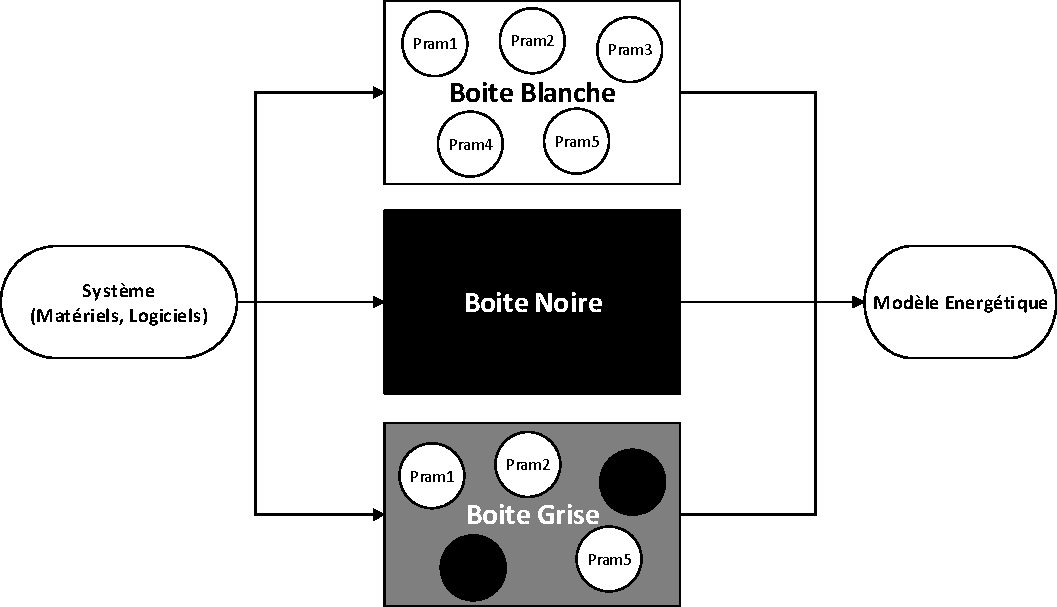
\includegraphics[scale=0.60]{chapitre4/chap4Fig/modelling-approaches.pdf}
 \caption{Les approches de modélisation d'énergie.}
 \label{fig:modelling-approaches}
\end{figure}

\subsection{Niveau de modélisation}
Lorsqu'une requête SQL est soumise à un SGBD, elle sera traduite en un arbre d'opérateurs algébriques puis en plan d'exécution. L'optimiseur de requêtes applique des fonctions analytiques pour trouver le meilleur plan d'exécution. Ensuite, la requête sera exécutée suivant un mode itératif (pipeline), où un ensemble d'opérateurs algébriques s'exécutent en même temps lorsqu'il y a des données à traiter.
Intuitivement, la modélisation d'énergie d'une requête,  peut se faire à trois niveaux :

\begin{enumerate}
 \item \textbf{Niveau requête.} Considérer les caractéristiques de la requête elle-même, telles que le nombre d'entrées/sorties requises pour exécuter la requête. Ce niveau est facile à mettre en œuvre mais ne garantis pas la précision désirée.
 \item \textbf{Niveau pipeline.} Considérer les caractéristiques de l'ensemble d'opérateurs qui s'exécutent simultanément. Le défi dans ce niveau est la détermination de ces opérateurs.
 \item \textbf{Niveau opérateur.} Considérer les caractéristiques de l'opérateur individuellement. La modélisation à ce niveau exige des détails sur les opérateurs et leurs implémentations, ce qui rend le processus complexe.
\end{enumerate}

Le bon choix du niveau de modélisation est crucial pour la qualité du modèle final. Ce choix peut se faire à l'aide d'une étude expérimentale comme décrit dans la section précédente. %DONE no comprendo la derniere phrase

\subsection{Mode d'exécution des requêtes}
La plupart des SGBDs modernes sont des systèmes multi-utilisateurs où plusieurs utilisateurs peuvent se connecter à la BD et exécuter des requêtes de façon concurrente. Il incombe au SGBD de gérer la concurrence d'accès aux données, et de garantir la fiabilité des résultats des requêtes. Comme nous allons montrer, la consommation énergétique pour une seule requête n'est pas forcément la même pour un ensemble de requêtes qui s'exécutent en même temps en parallèle. Par conséquent, il existe deux modes d'exécution de requêtes à considérer dans la phase de conception d'un modèle de coût énergétique : (1) le mode isolé et (2) le mode concurrent.

\begin{enumerate}
 \item \textbf{Mode isolé.} Une seule requête est en train d'être exécutée de façon isolée par le SGBD dans une instance donnée. Ce mode est la base de toute conception d'un modèle de coût énergétique due à sa complexité réduite.
 \item \textbf{Mode concurrent.} Plusieurs requêtes sont en train d'être exécutées de façon concurrentes par le SGBD dans une instance donnée. Ce mode est plus générique que le premier et plus utile pour de nombreuses tâches de gestion de BD, à l'exemple du contrôle d'admission, l'ordonnancement des requêtes et de contrôle d'exécution. Cependant, la conception de ce mode est plus complexe.
\end{enumerate}

\section{Démarche pour la construction d'un modèle de coût énergétique}\label{DemarcheConstruction}
Dans cette section, nous présentons notre méthodologie pour créer un modèle de coût qui estime la consommation d'énergie d'une seule requête SQL.
Nous adoptons une approche logicielle basée sur une étude empirique pour trouver les paramètres clés ayant un impact sur l'énergie, et pour identifier le niveau adéquat pour modéliser l'énergie des requêtes. L'étude empirique permet aussi de sélectionner l'algorithme mathématique qui modélise mieux le comportement de l'énergie des requêtes SQL. Les principales étapes pour développer notre modèle de coût sont (cf. \ref{fig:costmodel-methodology}) :

\begin{itemize}
 \item \textbf{Identification des paramètres.} Afin de réduire la consommation d'énergie d'un système, nous devons d'abord mesurer la consommation d'énergie de ses composantes et identifier là où la plupart de l'énergie est dépensée. Ceci est la tâche de la phase d'extraction des paramètres du modèle. Elle prend comme entrée le matériel utilisé, le SGBD et la charge de requêtes.
 \item \textbf{Construction du modèle.} Les paramètres d'entrée sélectionnés précédemment sont utilisés pour construire le modèle de consommation d'énergie en utilisant des techniques \textit{analytiques} ou \textit{statistiques} telles que la régression, l'apprentissage automatique, etc. L'un des principales difficultés de cette étape est que certains paramètres importants du système tels que la consommation d'énergie d'un composant particulier, ne peuvent pas être mesurés directement. Les méthodes analytiques classiques peuvent ne pas produire des résultats précis dans de telles situations, les techniques d'apprentissage automatique peuvent donner de meilleurs résultats.
 \item \textbf{Validation et utilisation.} Le modèle doit être validé selon différents scénarios pour son adaptation à ses fins prévues. Il peut être utilisé a postériori comme une base pour prédire la consommation d'énergie des requêtes. Ces estimations peuvent ensuite être utilisées pour améliorer l'efficacité énergétique des SGBD, par exemple en incorporant le modèle dans des techniques d'optimisation telles que la conception physique, l'ordonnancement des requêtes, l'ajustement dynamique de la fréquence de la tension (DVFS), l'amélioration des algorithmes et ainsi de suite.
\end{itemize}

\begin{figure}
 \centering
 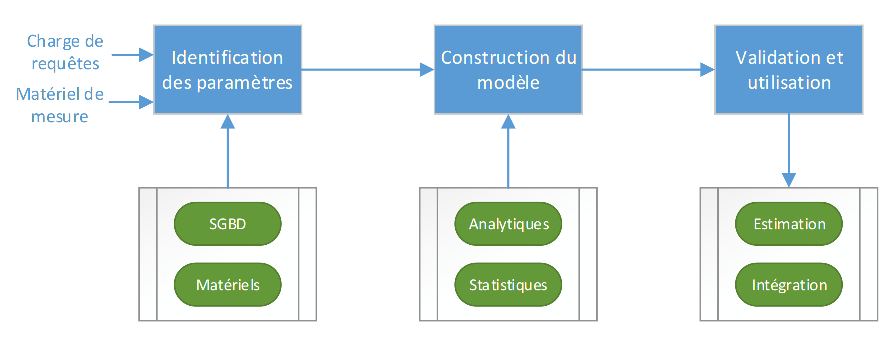
\includegraphics[scale=0.8]{chapitre4/chap4Fig/costmodel-methodology.eps}
 \caption{Les étapes de développement de notre modèle de coût énergétique.}
 \label{fig:costmodel-methodology}
\end{figure}

\subsection{Nos hypothèses}
% DONE Stéphane "le méticuleux" m'a déconseillé l'utilisation des abrévéations p. ex./c-a-d .. a toi de voir
Dans notre étude, et à cause de la complexité du problème traité, nous limitons les possibilités liées à l'environnement. La multitude des environnements (p. ex. centralisé, distribué et parallèle), des SGBD (p. ex. relationnel, NoSQL ou NewSQL) ou encore des requêtes (p. ex. sélection et mise à jour) rend la démarche plus complexe. Dans notre travail, nous considérons les hypothèses suivantes :
%DONE remplir les points de suspension. A moin avis ne pas justifier car c'est evident, dire simplement, Nous présentons, ci-dessous, les hypothèses que nous avons considérées pour établir ces MdC.
\begin{enumerate}
 \item L'environnement de travail est centralisé, la BD est déployée dans une seule station de travail. Par conséquent, le coût de communication est ignoré.
 \item Nous ne considérons pas des requêtes de définition de données (p. ex. \texttt{CREATE}, \texttt{DROP}, \texttt{ALTER}) ou encore de requêtes de manipulation de données (p. ex. \texttt{INSERT}, \texttt{DELETE}, \texttt{UPDATE}). Les requêtes considérées sont de type transactionnel et analytique, ayant la forme suivante :
 %\begin{lstlisting}[caption=An OCL structural rule, label=lst:listingocl]
 \begin{lstlisting}[language=Sql]
SELECT [DISTINCT ou ALL] colonnes
FROM tables
[WHERE predicats]
[GROUP BY expression]
[HAVING condition]
[ORDER BY colonnes]
\end{lstlisting}
 \item Les requêtes sont exécutées de façon isolée et concurrente (c-à-d parallélisme inter-requêtes).
 \item Le cache est vidé entre l'exécution des requêtes.
\end{enumerate}

\subsection{Identification des paramètres}
La première étape de notre approche est l'identification des paramètres clés de notre modèle qui influencent sur la consommation d'énergie des requêtes. L'identification est réalisée suivant une approche d'apprentissage automatique. Cette stratégie expérimentale est utilisée lorsque les paramètres du $\mathcal{BNF}$ sont inconnus au préalable. Dans cette stratégie, nous testons l'exécution de plusieurs requêtes simples et complexes, isolées et concurrentes, dans différentes BD et de tailles différentes, puis nous observons les paramètres liés à la stratégie d'exécution des requêtes, les caractéristiques de la BD et le matériel utilisé.

\subsubsection{Effet de stratégie d'exécution des requêtes}
Pour étudier l'effet de la stratégie d'exécution des requêtes sur la consommation d'énergie, nous commençons par montrer un exemple de la requête \textit{Q9} du benchmark TPC-H \cite{TPCH}. La \ref{fig:tpch-q9-sql} montre la syntaxe de cette requête qui détermine le bénéfice de la vente d'une ligne de pièces, groupé par la nation et l'année des fournisseurs.

Les ensembles de données et la configuration du système que nous avons utilisés dans nos expérimentations peuvent être trouvés dans la \ref{sec:experiment}.
La \ref{fig:tpch10-set1-q9-power} montre la consommation d'énergie active pendant l'exécution de la requête qui a débuté à la 10\textsuperscript{ème} seconde et a fini à la 143{ème} seconde. Nous pouvons y distinguer trois segments différents qui s'avèrent correspondre à la segmentation en \textit{pipelines}. Ces derniers permettent l'exécution simultanée d'une séquence contiguë d'opérateurs SQL souvent implémentés selon un modèle itératif \cite{Connolly05}.

La segmentation en pipelines du plan d'exécution de la requête \textit{Q9} est montrée dans la \ref{fig:tpch10-set1-q9-tree}. Il y a 7 pipelines dont l'ordre d'exécution est déterminé par leurs opérateurs \textit{bloquant} (p. ex. $PL6$ ne peut pas commencer avant que $PL5$ soit terminé). Bien que la requête a sept pipelines différents, seulement quatre sont importants dans notre discussion (les autres terminent très rapidement).
La détermination des segments énergie-pipelines est effectuée à l'aide du \textit{module de surveillance SQL temps réel} intégré dans le SGBD \cite{Sergey09}, qui nous donne en temps réel les statistiques à chaque étape du plan d'exécution avec le temps écoulé. Sur la base de ces informations, nous avons segmenté l'intervalle de l'énergie en pipelines correspondants.

\begin{figure}
\begin{lstlisting}[language=sql]
select nation, o_year, sum(amount) as sum_profit
from
	(
		select
			n_name as nation, extract(year from o_orderdate) as o_year,
			l_extendedprice * (1 - l_discount) - ps_supplycost * l_quantity as amount
		from
			part, supplier, lineitem,
			partsupp, orders, nation
		where
			s_suppkey = l_suppkey and ps_suppkey = l_suppkey
			and ps_partkey = l_partkey and p_partkey = l_partkey
			and o_orderkey = l_orderkey and s_nationkey = n_nationkey
			and p_name like '%sandy%'
	) as profit
group by nation, o_year
order by nation, o_year desc;
\end{lstlisting}
  \caption{La requête \textit{Q9} issue du benchmark TPC-H.}\label{fig:tpch-q9-sql}
\end{figure}

Si l'on compare les intervalles de changement de la consommation d'énergie avec le changement des pipelines dans la \ref{fig:tpch10-set1-q9}, nous pouvons voir que \textit{lorsqu'une requête passe d'un pipeline à l'autre, sa consommation d'énergie également change}. Au cours de l'exécution d'un pipeline, la consommation d'énergie a généralement tendance à être stable.
L'hypothèse faite par Xu \textit{et al.} stipulant que lors de l'exécution d'une seule requête dans un système, le coût de l'énergie est stable (steady state) \cite{Xu12} s'avère donc être fausse. En effet, de nombreuses requêtes ont différents segments de consommation d'énergie au cours de leur exécution. Ceci est dû au fait que l'estimation de Xu \textit{et al.} a été réalisée au niveau de la requête. Pour avoir des modèles de coûts d'énergie plus précis, l'estimation doit être effectuée au niveau plus fin qui constitue les pipelines.

\begin{figure}[!ht]
  \centering
  \subfloat[La segmentation de la consommation d'énergie suivant les pipelines\label{fig:tpch10-set1-q9-power}]{
    \centering
    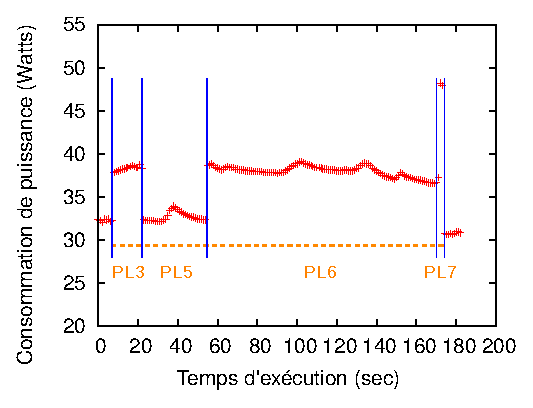
\includegraphics[width=0.5\textwidth]{chapitre4/chap4Fig/tpch10-set1-q9-5.eps}
  }
  \quad
  \subfloat[La segmentation du plan d'exécution suivant les pipelines\label{fig:tpch10-set1-q9-tree}]{
    \centering
    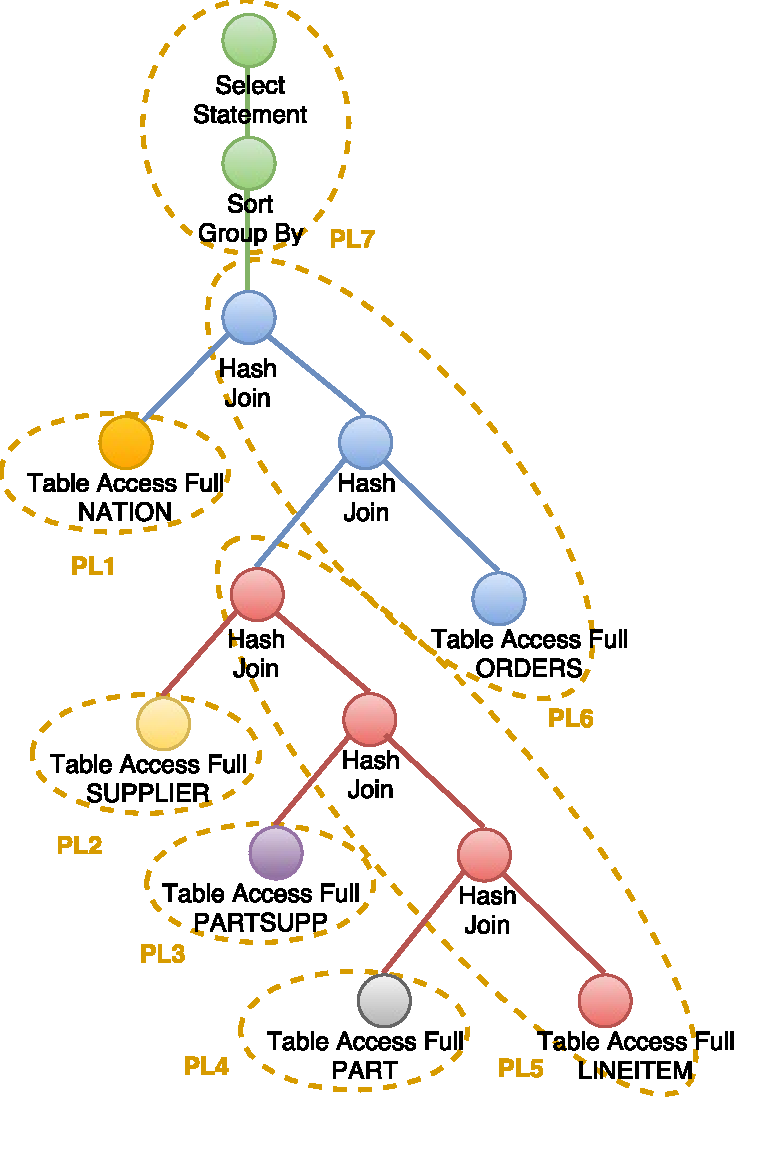
\includegraphics[width=0.4\textwidth]{chapitre4/chap4Fig/tpch-10go-q9-plan.pdf}
  }
  \caption{La consommation d'énergie et le plan d'exécution de la requête \textit{Q9} issue du benchmark TPC-H avec l'annotation des pipelines correspondante.}\label{fig:tpch10-set1-q9}
\end{figure}

\subsubsection{Effet de la taille de BD}
Habituellement, nous admettons le fait suivant : \textit{<< grande taille, plus d'énergie >>}. Pour vérifier ce fait, nous menons des expérimentations, en termes de consommation de puissance active, en tenant compte des requêtes du benchmark TPC-DS \cite{TPCDS} avec deux ensembles de données. Le premier ensemble est de taille 10 Go et le second de 100 Go.
Nous voyons clairement dans le \ref{tab:query-comp}, que les requêtes interrogeant une petite taille de données peuvent  \textit{parfois} consommer plus de puissance que des requêtes interrogeant une grande taille de données. Nous avons créé un autre jeu de données du benchmark TPC-H avec des requêtes modifiées et nous avons trouvé le même comportement (les résultats ne sont pas présentés car ils sont très semblables). Nous notons ici que le plan d'exécution généré par le SGBD pour chaque requête est le même dans les deux ensembles de données.

\begin{table}[]
\centering
\caption {Comparaison de la consommation de puissance active des requêtes du benchmark TPC-DS avec différentes tailles de BD.} \label{tab:query-comp}
%\rowcolors{0}{}{lightgray}
\begin{tabular}{ccc}
%\begin{tabular}{@{}ccc@{}}
\toprule
\multirow{2}{*}{\textbf{Requête}} & \multicolumn{2}{c}{\textbf{Puissance d'électricité (W)}} \\ \cmidrule(l){2-3} 
                                & \textbf{10 Go}                  & \textbf{100 Go}                 \\ \midrule
	$Q4$           & 44,6       & 40,6        \\ 
    $Q9$           & 42,7       & 37,4        \\ 
    $Q11$          & 43,9       & 40,9        \\ 
    $Q39$          & 42,9       & 38,5        \\ 
    $Q48$          & 47,0       & 37,9        \\     
    $Q72$          & 36,4       & 34,1        \\ 
    $Q88$          & 43,3       & 37,6        \\ \bottomrule
\end{tabular}
\end{table}

Nous expliquons ce constat par le fait que pour certaines requêtes, la lecture de gros fichiers de données a besoin de plus de tâches d'E/S. Ainsi, lorsque les résultats intermédiaires ne peuvent pas être stockés dans la mémoire, ils seront écrits sur le disque et lus plus tard. Cette manœuvre se traduit par plus de temps d'attente de CPU, car la requête passe son temps dans la lecture/écriture de ses données plus que dans le traitement de ses tuples. Ainsi, les requêtes dominées par des coûts d'E/S ont moins de consommation d'énergie. De l'autre côté, lorsque les données sont de petite taille, la lecture de données termine rapidement et dans son temps restant, l'exécution de la requête est dominée par le traitement du processeur, ce qui peut se traduire par une forte consommation d'énergie.

Cette observation nie la prémisse faite par Xu \textit{et al.} stipulant que la consommation d'énergie marginale (énergie active) d'une requête est positivement liée à la taille de données interrogées \cite{Xu13}. En effet, nous avons trouvé beaucoup de contre-exemples où des requêtes ont une consommation différente indépendamment de la taille de données, comme indiqué précédemment dans le \ref{tab:query-comp}.

Le coût du CPU et le coût des E/S fournis par le SGBD sont candidats pour être les paramètres du modèle pour les raisons suivantes :
\begin{itemize}
 \item ils sont déjà calculés et disponibles à partir du SGBD optimiseur,
 \item ils couvrent un large éventail d'opérateurs SQL mises en œuvre par les SGBD.
\end{itemize}
Nous avons décidé d'utiliser les coûts CPU et E/S en tant que paramètres dans notre modèle, contrairement à Kunjir \textit{et al.} \cite{Kunjir12} qui utilisent le débit et la taille de données comme paramètres pour modéliser la consommation de puissance maximale (peak power).%DONE compléter la ref

\subsubsection{Effet du mode d'exécution des requêtes}
Nous étudions l'effet du mode d'exécution des requêtes (isolé ou concurrent) sur la consommation d'énergie du système. Pour cela, nous utilisons les données et les charges de requêtes issues du benchmark TPC-H. Nous avons créé de nouvelles charges de requêtes pour chaque mode d'exécution à partir des 22 requêtes d'origine en se basant sur un taux de multiprogrammation donné. 
%DONE vérifier cette derniere phrase

\begin{definition}
Un taux de multiprogrammation (\gls{MPL}) est défini comme le nombre de requêtes exécutées en même temps à un instant donné.
\end{definition}
La charge de requêtes contient les mêmes requêtes, mais avec différentes instances. Nous avons exécuté les charges de requêtes et enregistré leurs consommation d'énergie. Ensuite, nous avons calculé la puissance minimale, maximale et moyenne pour chaque MPL. Les résultats sont présentés dans la \ref{fig:mpls-power}. Nous notons que le taux de multiprogrammation \textit{x} signifie que \textit{x} requêtes s'exécutent simultanément.

\begin{figure}
 \centering
 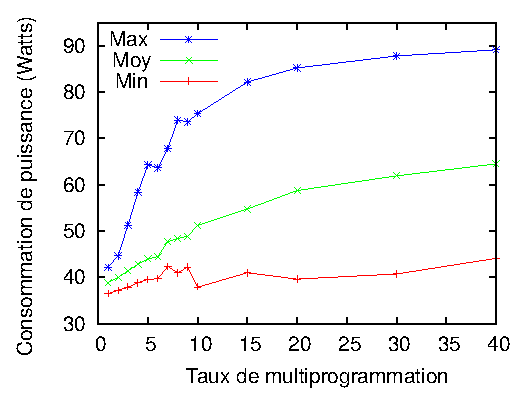
\includegraphics[scale=0.9]{chapitre4/chap4Fig/mpls-power.eps}
 \caption{Variation de la consommation d'énergie de la charge de requêtes suivant les différents taux de multiprogrammation (MPLs).}
 \label{fig:mpls-power}
\end{figure}

Comme prévu, la consommation d'énergie augmente à mesure que l'on augmente le degré de concurrence, car le système devient plus chargé. En fait, le système atteint son débit maximal à \textit{MPL = 40} et consomme sa puissance maximale (95 Watts) tel que mentionné par le fabriquant du matériel. De plus, on observe une grande différence entre le minimum, le maximum, et la moyenne de consommation d'énergie du même MPL. Ainsi, la modélisation pour des requêtes s'exécutant en mode concurrent est largement plus difficile que pour une seule requête autonome. Par conséquent, la considération du mode d'exécution dans la modélisation est cruciale pour une prédiction avec précision de la puissance d'une charge de requête.

Inspiré par les constats des sections précédentes, nous avons conçu et mis en œuvre un modèle d'énergie à base de coût. %L'idée de base de ce modèle est de
La \ref{fig:power-model-building} montre le flux de travaux de notre processus de modélisation d'énergie.
Les caractéristiques de notre modèle comprennent : (1) la segmentation d'un plan d'exécution en un ensemble de segments d'énergie/pipelines suivant les opérateurs bloquants et semi-bloquants, (2) l'utilisation du coût CPU et E/S des pipelines et de l'énergie mesurée on mode \textit{hors ligne} pour construire le modèle et (3) l'estimation de l'énergie des futures requêtes en mode \textit{en ligne} basée sur le modèle de coût final. Ainsi, nous bénéficions des avantages suivants :
\begin{itemize}
 \item nous ne nous appuyons pas sur type d'opérateur SQL ou sur son implémentation physique, car la modélisation de chaque opérateur algébrique est complexe et diffère d'un SGBD à un autre.
 \item notre modèle peut être facilement intégré dans l'optimiseur des SGBD existants.
\end{itemize}

\begin{figure}
 \centering
 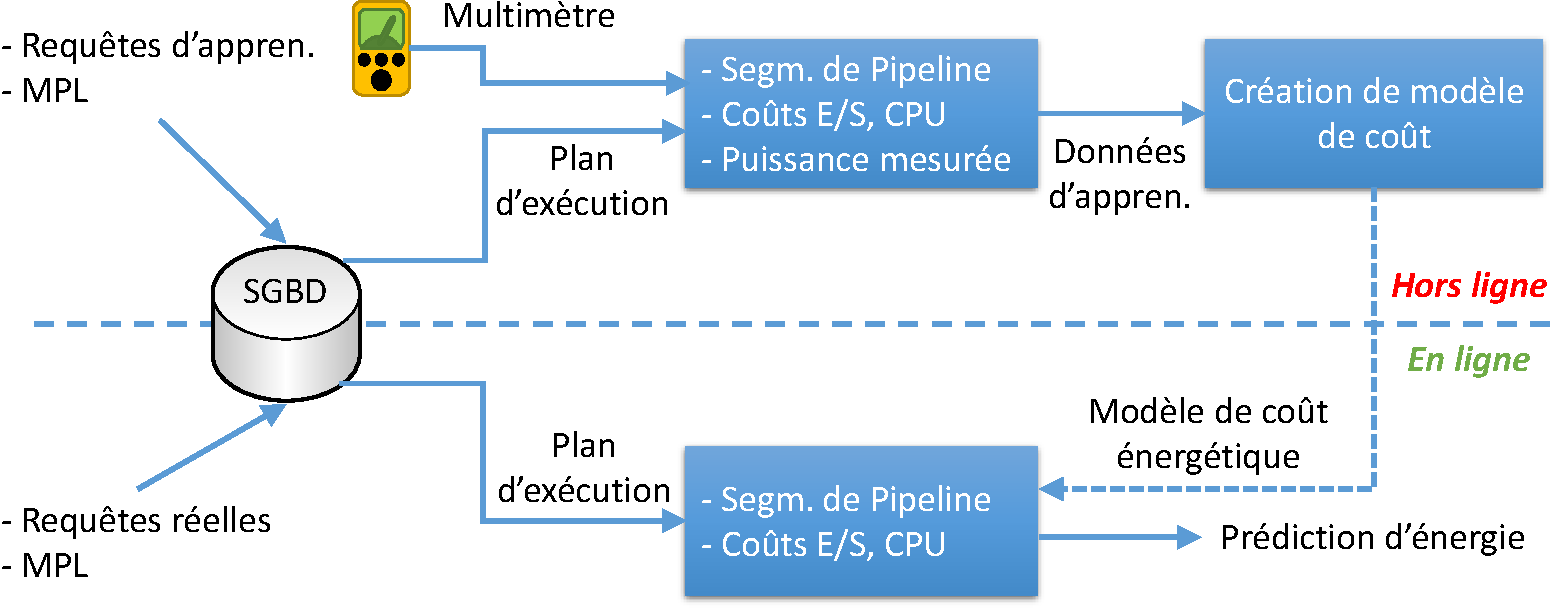
\includegraphics[scale=0.55]{chapitre4/chap4Fig/power-model-building.pdf}
 \caption{Le processus de conception du modèle de coût énergétique.}
 \label{fig:power-model-building}
\end{figure}

Dans les sections suivantes, nous détaillons chaque étape de notre processus de modélisation.

\subsection{Segmentation en pipelines}
La deuxième étape de notre approche est la segmentation en pipelines. Quand une requête est soumise à un SGBD, l'optimiseur de requêtes choisit un plan d'exécution. Un plan est un arbre composé d'un ensemble d'opérateurs physiques, tel que la lecture, la jointure ou le tri. La \ref{fig:tpch10-set1-q9-tree} présente un exemple de plan d'exécution renvoyée par l'optimiseur de requêtes. Un opérateur physique peut être \textit{bloquant} ou \textit{non bloquant}.
\begin{definition}
Un opérateur est bloquant s'il ne peut produire aucun tuple sans lire au moins une de ses entrées (p. ex. l'opérateur de tri).
\end{definition}
Basé sur la notion des opérateurs bloquant/non bloquant, nous décomposons le plan d'exécution en un ensemble de pipelines délimités par les opérateurs bloquants. Ainsi, un pipeline est défini comme suit.
\begin{definition}
Un pipeline est un ensemble d'opérateurs s'exécutant simultanément \cite{li12}.
\end{definition}
Comme dans les travaux précédents \cite{chaudhuri04, luo04}, les pipelines sont créés de manière inductive, à partir des opérateurs feuilles du plan à l'instar de l'accès séquentiel et l'accès par index. Chaque fois que nous rencontrons un opérateur bloquant, comme le tri et le groupage, le pipeline en cours se termine et un nouveau commence. Pour une jointure de hachage, l'opérateur de jointure est inclus dans le pipeline du nœud de calcul de jointure (\textit{probe phase} en anglais), et le nœud de la construction de la table de hachage (\textit{build phase}) est la racine d'un autre pipeline. Pour une opération de jointure par tri-fusion, les pipelines contenant ses nœuds d'entrée et l'opérateur de jointure sont réunis pour créer un seul pipeline. Pour une jointure par boucles imbriquées ou boucles imbriquées avec index, les nœuds externes, l'opérateur de jointure et toute sa sous-arborescence des nœuds intérieurs font partie d'un même pipeline.
La définition donnée ci-dessus peut être étendue à d'autres opérateurs physiques. L'\ref{algo:pl-segmentation-algo} illustre un pseudo code de ce principe avec quelques opérateurs, une implémentation en C++ est mentionnée dans le \ref{chap5}. 
Par conséquence, le plan d'exécution d'origine peut être considéré comme un arbre de pipelines. La \ref{fig:tpch10-set1-q9-tree} montre le plan d'une requête ayant 7 pipelines :
\begin{enumerate}
 \item Les pipelines $PL1$, $PL2$, $PL3$, $PL4$ font la lecture séquentielle des tables de données et construisent leur table de hachage en même temps. Ce sont des opérateurs bloquants.
 \item Le pipeline $PL5$ fait la jointure par hachage (opérateurs non-bloquant) entre la table \texttt{LINEITEM} et le $PL1$ puis le résultat avec les autres pipelines. À la fin, le pipeline construit la table de hachage du résultat final.
 \item Le pipeline $PL6$ fait la jointure par hachage entre $PL5$ et la table \texttt{ORDERS} puis le résultat avec le $PL1$.
 \item Le pipeline $PL7$ calcule l'opérateur bloquant qui est le tri de $PL6$ et affiche le résultat final de la requête.
\end{enumerate}

\begin{algorithm}
\caption{Algorithme de segmentation des pipelines}
\label{algo:pl-segmentation-algo}
\begin{algorithmic}[1]
\Require  $Plan$ \Comment{un plan d'exécution d'une requête SQL contenant des opérateurs $OP$}
\Ensure $PL$ \Comment{une liste contenant la segmentation des pipelines}
\State $PLActuel \leftarrow \emptyset$;
\ForAll {opérateur $OP_i \in Plan$}
    \If{$estFeuille(OP_i)$}
        \State $j \leftarrow i$;
		\While{$j \in Plan$ et $OP_j \neq \text{<< Tri >>}$ et $OP_j \neq \text{<< Agrégation >>}$ et $OP_j \neq \text{<< Matérialisation >>} \cdots$}
			\State $PLActuel \leftarrow PLActuel + OP_j$;
			\State $j \leftarrow j+1$;
		\EndWhile
		\State $PL \leftarrow PLActuel + PL$;
		\State $PLActuel \leftarrow \emptyset$;
	\EndIf
\EndFor
\State
\Return $PL$;
\end{algorithmic}
\end{algorithm}

En outre, sur la base de notre analyse, nous avons constaté que le SGBD exécute les pipelines dans un ordre séquentiel, donc il n'y a pas de pipeline en concurrence.
Comme nous l'avons mentionné auparavant, nous décomposons le plan en un ensemble de pipelines, et nous les ordonnons sur la base des informations fournies par le module de surveillance SQL temps réel du SGBD. Ce module affiche des statistiques en temps réel afin d'identifier les problèmes de performance d'exécution des requêtes avec longue durée. Cela permet aux administrateurs de BD d'analyser l'exécution des requêtes et de décider des stratégies d'optimisation les plus appropriées \cite{Sergey09}. La \ref{fig:tpch-q9-sqlmonitor} montre une partie de ce module, les informations les plus importantes sont :

\begin{itemize}
 \item La colonne \texttt{Operation} indique le type d'opération SQL dans le plan d'exécution, le nom associé à cette opération est affiché dans la colonne \texttt{Name}. Par exemple, le nom de la table \texttt{LINEITEM} est associé à l'opération de lecture \texttt{TABLE ACCESS FULL}.
 \item La colonne \texttt{Estimated Rows} affiche les cardinalités estimées pour chaque opération lors de la génération des plans d'exécutions. Idem pour \texttt{Cost} qui affiche le coût estimé des opérations en terme de CPU et d'E/S, les valeurs sont cumulées de bas vers le haut et son unité de mesure n'est pas spécifié par Oracle.
 \item La colonne \texttt{Actual Rows} affiche les cardinalités réelles de chaque opération après l'exécution de la requête.
 \item La colonne \texttt{Timeline} est la plus importante dans notre travail. Elle affiche le temps de début d'exécution de l'opérateur pour la première fois et sa durée totale, ce qui permet d'identifier et de segmenter les pipelines. La colonne \texttt{Execution} indique le nombre de fois que l'opérateur a été exécuté.
 \item Les colonnes \texttt{Memory (Max)} et \texttt{Temp (Max)} affichent la taille mémoire et l'espace temporaire maximaux qui ont été consommés durant l'exécution de l'opérateur.
 \item La colonne \texttt{IO Requests} indique le nombre de demandes de lecture et d'écriture sur un support de stockage externe. Selon la figure, des demandes de lecture ont été effectués par les opérateurs de lecture, et des demandes de lecture et écriture par l'opérateur \texttt{HASH JOIN}. Les demandes par l'opérateur de jointure sont dues à la saturation de l'espace mémoire alloué pour le SGBD.
 \item La colonne \texttt{CPU Activity (\%)} affiche la portion d'utilisation de la ressource CPU par chaque opérateur. Dans notre exemple, le CPU a été utilisé par les opérateurs de jointure et l'opérateur de tri \texttt{SORT GROUP BY}.
\end{itemize}

Cette fonctionnalité de surveillance des requêtes est aussi disponible dans d'autres SGBD, à l'exemple de SQL Server \cite{Agarwal09}, PostgreSQL\footnote{http://www.postgresql.org/docs/current/static/sql-explain.html} et MySQL \cite{MySQL10}.

\begin{figure}
 \centering
 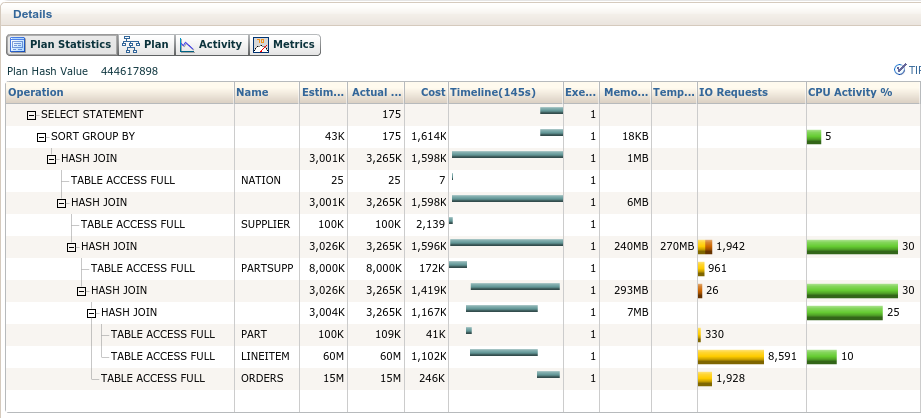
\includegraphics[scale=0.65]{chapitre4/chap4Fig/tpch-q9-sqlmonitor.png}
 \caption{Aperçu du module de surveillance SQL temps réel d'Oracle.}
 \label{fig:tpch-q9-sqlmonitor}
\end{figure}

\subsubsection{Cas des requêtes concurrentes}
Supposons que nous avons une charge de requêtes $q_1, q_2, \cdots, q_n$. Après avoir segmenté leurs plans d'exécution en un ensemble de pipelines, la charge de requêtes peut être considérée comme de multiples phases de mixes de pipelines. Ceci est illustré par la \ref{fig:concurent-pipelines}. Dans cet exemple, nous avons une charge de 5 requêtes $q_1, \cdots, q_5$. Après la segmentation de leurs plans, $q_1$ est représentée comme une séquence de 3 pipelines $P_{11} P_{12} P_{13}$, $q_2$ est représentée comme une séquence de 4 pipelines $P_{21} P_{22} P_{23} P_{24}$, et ainsi de suite pour les autres requêtes. Nous utilisons $PL{ij}$ pour désigner le $j^{ième}$ pipeline de la $i^{ième}$ requête, et nous utilisons $ph_{k}$ pour désigner la phase où un certain pipeline $PL_{ij}$ termine son exécution. Comme nous le voyons, nous pouvons identifier un nouveau mix de pipelines dès qu'un certain pipeline termine son exécution. Dans notre exemple, à la fin, nous aurons 14 mixes de pipelines, séparés par les lignes bleues en pointillés qui indiquent le temps de fin d'exécution de chaque pipeline.

\begin{figure}
 \centering
 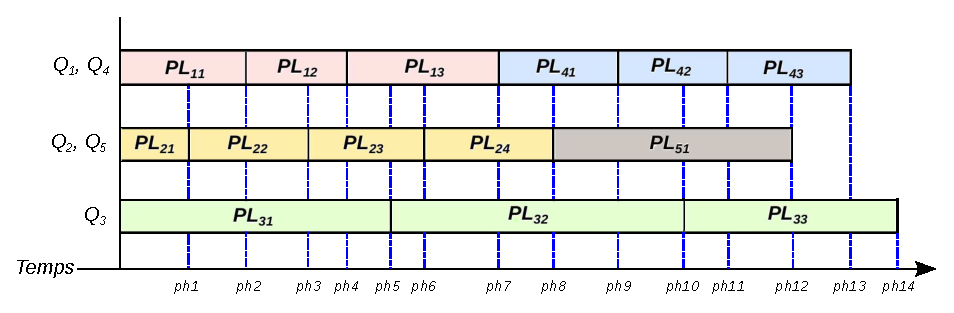
\includegraphics[scale=0.9]{chapitre4/chap4Fig/concurent-pipelines.eps}
 \caption{Les segmentation des pipelines d'une charge de requêtes concurrentes.}
 \label{fig:concurent-pipelines}
\end{figure}

\begin{algorithm}
\caption{Algorithme de prédiction}
\label{algo:prediction-algo}
\begin{algorithmic}[1]
\Require  $W = \{q_1, \cdots, q_n\}$ \Comment{une charge de $n$ requêtes SQL}
\Ensure $P_w$ \Comment{la consommation d'énergie estimée pour la charge $W$}
\ForAll {requête $i \in W$}
    \State $Plan_i \leftarrow GetPlan(i)$;
    \State $PL_i \leftarrow GetPipelines(Plan_i)$;
\EndFor
\State
$PLMixActuel \leftarrow \emptyset$;
\ForAll {requête $i \in W$}
    \State $PLMixActuel \leftarrow PLMixActuel + PL_{i1}$;
\EndFor
\State

\While{$PLMixActuel \neq \emptyset$}
	\State $PL_{ij} \leftarrow PlusCourtPipeline(PLMixActuel)$;
	\State $t_{min} \leftarrow t_{ij}$;
	\State $Co\hat{u}t \leftarrow 0$;
	\ForAll {$PL_{ik} \in CurrentMix$}
		\State $Co\hat{u}t \leftarrow Co\hat{u}t + Co\hat{u}t_{ik} \times \frac{t_{min}}{t_{ik}}$;
	\EndFor
	\State $P_w \leftarrow P_w + EstimePuissance(Co\hat{u}t)$;
	\State Retirer $PL_{ij}$ depuis $MixActuel$;
	\If{$aPlusDePipelines(PL_i)$}
		\State $PLMixActuel \leftarrow PLMixActuel + PL_{i(j+1)}$;
	\EndIf
\EndWhile

\State
\State
\Return $P_w$;
\end{algorithmic}
\end{algorithm}

L'exécution de la charge de requêtes est assimilée à l'exécution d'une suite de mixes de pipeline. L'exécution de chaque mix est appelée une phase de pipeline. Un changement de phase se produit quand un pipeline termine son exécution et un autre pipeline commence. Notre objectif est de déterminer les phases de pipeline et les transitions entre eux et d'estimer la quantité d'énergie consommée par chaque phase. La consommation d'énergie de la charge de requêtes est la consommation totale de toutes les phases. Cette idée est présentée dans l'\ref{algo:prediction-algo}.

Dans cet algorithme, nous générons d'abord le plan d'exécution $Plan_i$ pour chaque requête $Q_i$ en appelant l'optimiseur de requêtes, puis nous créons la segmentation de pipelines $PL_i$ de chaque $Plan_i$. Le premier pipeline $PL_{i1} $ dans chaque $PL_i$ est ajouté au mix en cours d'exécution $CurrentPLMix$. Ensuite, nous continuons l'exécution par phase tant que le mix actuel ne soit pas vide. Nous déterminons le pipeline $PL_{ij} $ avec le temps d'exécution le plus court $t_{min}$. Ensuite, nous calculons \textit{le coût énergétique du travail effectué} par chaque pipeline $PL_{ik} $ dans le mix actuel, en multipliant le coût de chaque pipeline par $\frac{t_{min}}{t_{ik}} $, où $t_{ik}$ est le temps d'exécution du pipeline $PL_{ik}$. Nous appelons la procédure d'estimation d'énergie pour obtenir l'énergie du mix de pipeline actuel, et nous retirons $P_{ij}$ du mix. Si $PL_i$ contient plus de pipelines après la fin d'exécution du $P_{ij}$, nous ajoutons le suivant $P_{i(j+1)}$ dans le mix en cours et nous répétons ce processus jusqu'à ce que toutes les requêtes de la charge sont terminées. La consommation d'énergie finale de la charge de requêtes est la somme de consommation de chaque phase.

\subsection{Modélisation des pipelines}
Après l'identification des paramètres de notre modèle et le niveau de modélisation. La prochaine étape consiste à modéliser ces paramètres. Dans cette section, nous allons donner une formalisation pour notre approche. Ensuite, nous construisons notre modèle en identifiant le modèle mathématique qui décrit notre problème d'estimation d'énergie. Cette phase de construction combine les paramètres identifiés dans les sections précédentes avec une méthode d'apprentissage automatique pour trouver le meilleur modèle (boite grise).

\subsubsection{Coût CPU et E/S des pipelines}
Dans un SGBD traditionnel, le coût d'exécution de la requête est traité comme une combinaison linéaire de trois composantes : le coût du CPU, d'E/S et le coût de la communication \cite{Xu13}. Inspiré par cette méthodologie, nous proposons d'utiliser ces coûts pour modéliser les pipelines des requêtes.
Pour une charge de requête donnée, l'optimiseur de requêtes est responsable de l'estimation des coûts CPU et d'E/S. Notre stratégie pour la modélisation des pipelines est de profiter des modèles de coûts qui sont déjà intégrés dans les SGBD pour l'optimisation des requêtes. Dans un SGBD, pour traiter les tuples, chaque opérateur appartenant à un pipeline doit effectuer des tâches de CPU et/ou d'E/S. Le coût de ces tâches représente le << \textit{coût du pipeline} >>, qui est la puissance d'électricité active censée être consommée afin de terminer les tâches. Dans cette thèse, nous nous concentrons sur une configuration de serveur centralisé et laissons l'étude des BD distribuées pour les futurs travaux. Ainsi, le coût de la communication peut être ignoré. Plus formellement, pour une charge de requête donnée $W$ composée par des requêtes $Q$, notre modèle de coût énergétique pour $W$ est défini comme suit :
\begin{equation}
Puissance(W) = \sum_{i=1}^{n} Puissance(Q_i)
\end{equation}
Soit $Q_i$ une requête composée de $p_i$ pipelines $\{PL_1, PL_2, \dots, PL_p\}$. Le coût de l'énergie $Puissance(Q_i)$ de la requête $Q_i$ est donné par l'équation suivante :
\begin{equation}
Puissance(Q_i) = \frac{\sum_{j=1}^{p} Puissance(PL_j) * Time(PL_j)}{Time(Q_i)}
\end{equation}
$Time(PL_j)$ et $Time(Q_i)$ représentent respectivement, le temps d'exécution du pipeline $j$ et la requête $Q_i$. Ces deux facteurs sont complètement ignorés par Xu \textit{et al.} \cite{Xu13}. Dans notre modèle, le temps est un facteur important pour déterminer le pipeline dominant par les coûts CPU ou E/S dans une requête. Bien que le module statistique du SGBD nous fournisse ces informations, nous allons utiliser le temps d'exécution réel des requêtes afin de tester la qualité de notre modèle.

Notez que le coût d'un pipeline $j$ doit également être décomposé car il peut impliquer plusieurs opérations algébriques. Soit $n_j$ le nombre de ces opérations ($\{OP_1, OP_2, \dots, OP_n\}$). Le coût énergétique $Puissance(PL_j)$ d'un pipeline $j$ est donné par l'équation suivante :
\begin{equation} \label{eq:cost-model}
Puissance({PL_j}) = \beta_{cpu} \times \sum_{k=1}^{n_j} COUT\_CPU_k + \beta_{es} \times  \sum_{k=1}^{n_j} COUT\_ES_k
\end{equation}
Où $\beta_{cpu}$ et $\beta_{es}$ sont les paramètres du modèle (les unités des coûts énergétiques).

Pour une requête donnée, l'optimiseur utilise le plan d'exécution, les estimations de cardinalité et les formules pour les opérateurs afin de générer les valeurs des différents types d'opérations CPU et d'E/S. Il convertit ensuite ces valeurs en temps en utilisant des paramètres spécifiques au système, tels que la vitesse du processeur et la vitesse du transfert E/S. Par conséquent, dans notre modèle, nous prenons les estimations de CPU et d'E/S avant de les convertir en temps.
Les paramètres du système sont calculés à la création de la BD, et pourraient être peu fiables. Suivant les recommandations du fournisseur de SGBD, nous calibrons ces paramètres pour assurer la précision de l'estimation des ressources et  l'optimalité du plan d'exécution.

Le $COUT\_CPU$ est le nombre estimé de \textit{Cycle de CPU} et de \textit{lecture du cache mémoire} nécessaires au SGBD pour l'exécution de l'opérateur spécifié. De même, le $COUT\_ES$ est le nombre estimé d'\textit {E/S} nécessaire au SGBD pour l'exécution de l'opérateur spécifié.

Dans la littérature, l'estimation de ces deux coûts peut se réaliser suivant deux catégories de techniques : (1) techniques basées sur des fonctions analytiques et (2) techniques basées sur l'optimiseur de requêtes du SGBD \cite{Boukhalfa09Phd}. La première catégorie de techniques \cite{Boukorca15, Kerkad12a, Bouchakri11a} définit une fonction analytique pour calculer le coût d'une requête à partir d'un plan d'exécution prédéfini. À chaque opérateur algébrique, une formule qui prend en entrée des paramètres et des statistiques de la BD est utilisée pour le calcul de coût. L'avantage de cette méthode réside dans la facilité et la rapidité de la mise en œuvre et du calcul, mais elle reste limitée par les hypothèses simples et parfois irréalistes. De plus, elle ne garantit pas l'optimalité  du plan de la requête choisie. Par conséquent, cette méthode ne répond pas aux critères régissant la construction d'un modèle de coût énergétique de qualité, qui ont été décrits dans la \ref{sec:PourquoiModelCout}.

La deuxième catégorie de techniques \cite{Bruno11, Chaudhuri97, Chaudhuri98} fait appel à l'optimiseur de requête du SGBD utilisé pour estimer le coût d'une requête. L'optimiseur évalue les différents plans d'exécution de la requête et retourne l'optimal avec son coût. Le plan et le coût sont fiables comme exigé par nos critères de modélisation. De plus, cette technique rend l'intégration de notre modèle dans un SGBD réel plus facile.

Dans le cadre de cette thèse, nous adaptons une technique appartenant à la deuxième catégorie. Comme indiqué précédemment, en utilisant les coûts CPU et E/S retournés par le SGBD, nous ne dépendons pas du type ou de l'implémentation des opérateurs SQL comme dans \cite{Xu13}. Par conséquent, notre modèle est portable et peut traiter des requêtes plus complexes comme celles du benchmark TPC-DS.

\subsubsection{Estimation des paramètres du modèle}
Le principal défi dans la résolution de l'\ref{eq:cost-model} est de trouver les paramètres du modèle $\beta_{cpu}$ et $\beta_{es}$. Notre méthodologie utilise la technique de régression pour calculer ces paramètres de coût.

La notion de régression est fondamentale dans toutes les sciences appliquées, elle consiste à analyser une relation entre deux variables quantitatives et à l'exploiter pour estimer la valeur inconnue de l'une à l'aide de la valeur connue de l'autre. Elle est couramment utilisée dans les techniques de gestion et de commercialisation, pour expliquer un chiffre d'affaires en fonction des dépenses publicitaires, effectuer des prévisions de bénéfices, de ventes, etc. Dans les sections suivantes, nous détaillons cette technique, et nous formalisons la démarche utilisée pour calculer les paramètres de notre modèle de coût.

\paragraph{Régression linéaire}
On étudie en régression deux variables quantitatives, dont l'une appelée variable \textit{expliquée}, est considérée comme \textit{dépendante} de l'autre, appelée variable \textit{explicative} ou \textit{indépendante}. On note habituellement la variable expliquée $Y$, et la variable explicative $X$. Un exemple de cette dépendance est lorsqu'on mesure la consommation d'une voiture à des vitesses choisies pour établir la relation entre la consommation (variable dépendante) et la vitesse (variable indépendante) \cite{Montgomery12, Neter96, Kutner04}.

On qualifie un modèle de régression de \textit{simple} lorsque qu'il y a une seule variable explicative. \`A l'inverse, on le qualifie de \textit{multiple} en présence d'au moins de deux variables explicatives. Le modèle de régression simple est une équation censée représenter cette relation entre les deux variables. Il s'écrit sous cette forme :
\begin{equation}
Y = f(X) + \epsilon
\end{equation}
La variable $Y$ est supposée être approximativement égale à une fonction $f$ de $X$, le terme $\epsilon$ caractérisant la marge d'erreur ou d'imprécision du modèle. L'objectif est de préciser la nature de la régression (la fonction $f$), de mesurer le degré d'imprécision (le terme $\epsilon$), de détecter les observations qui ne suivent pas le modèle et d'effectuer des prévisions de $Y$ pour différentes valeurs de $X$. Nous supposons d'abord que la nature de la liaison entre les deux variables est linéaire. Le modèle de régression s'exprime alors de la façon suivante :
\begin{equation}
y = \beta x + a + \epsilon
\end{equation}
Où $\beta$ et $a$ représentent les coefficients théoriques de la régression et leurs valeurs sont inconnues. L'estimation de ces coefficients peut se faire avec plusieurs méthodes. Parmi les méthodes les plus utilisées on trouve la méthode des moindres carrés.

\subparagraph{Critère des moindres carrés}
Supposons que les données de l'étude de la régression se présentent sous la forme d'une suite de $n$ couples $[x(i), y(i)]$, numérotés de $i = 1$ à $i = n$. Nous avons représenté sur la \ref{fig:least-squares} cet ensemble de données. L'objectif est de déterminer les coefficients de la droite $y = \beta x + a$, appelée \textit{droite de régression}, la plus proche possible des $n$ points.

\begin{figure}
 \centering
 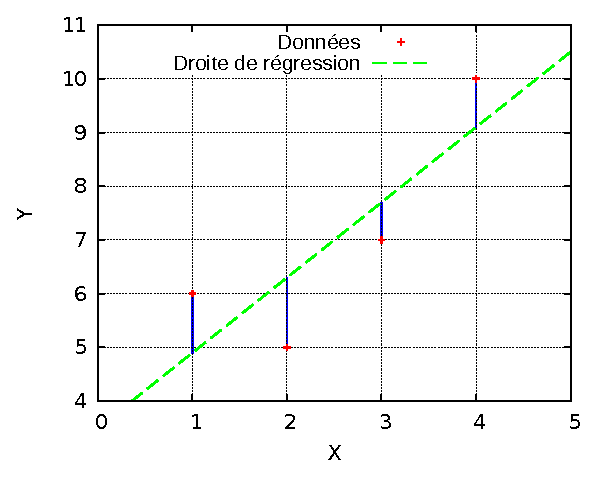
\includegraphics[scale=1.0]{chapitre4/chap4Fig/least-squares.eps}
 \caption{La régression linéaire par la méthode des moindres carrés.}
 \label{fig:least-squares}
\end{figure}

Plus précisément, il s'agit de reconstruire le mieux possible la variable $Y$ en fonction de la variable $X$ et de déterminer la droite de façon à ce que les termes d'erreur de la forme $\epsilon(i) = y(i) - [\beta x(i) + a ]$ soient les plus petits possible (les plus proches de 0). Ces termes $e(i)$ sont appelées aussi \textit{résidus}. Pour mesurer la proximité de la valeur 0 à ces erreurs, on cherche les coefficients $\beta$ et $a$ tel que la somme des carrés de ces termes soit minimale. Ces sommes sont représentées sur la \ref{fig:least-squares} par les longueurs des segments de couleur bleu.

%\begin{theorem}
Les estimations des coefficients de régression théoriques $\beta$ et $a$ sont telles que la somme des carrés des erreurs soit la plus petite possible. Elles sont données par les formules ci-dessous \cite{Neter96} :
 \begin{equation}
 \begin{aligned}
  %\beta = \frac{cov(x,y)}{S_{x}^{2}} = r(x,y) \frac{S_y}{S_x} \\
  \beta = \frac{ \sum_{i=1}^{n}(x_i-\bar{x})(y_i-\bar{y}) }{ \sum_{i=1}^{n} (x_i-\bar{x})^2} \; \text{et} \; a = \bar{y} - \beta \bar{x} \\
  \text{avec : } \; \bar{x} = \frac{1}{n} \sum_{i=1}^{n} x_i \; \text{et} \; \bar{y} = \frac{1}{n} \sum_{i=1}^{n} y_i
  \end{aligned}
 \end{equation}
%\end{theorem}

\subparagraph{Modèle énergétique en régression linéaire}
Appliquant les techniques expliquées dans les sections précédentes sur notre modèle de coût, le coût de l'énergie $Puissance_{PL_j} $ du pipeline $p_j$, avec une relation linéaire entre les paramètres du modèle, est calculé comme suit :
\begin{equation} \label{eq:lin-reg-equation}
Puissance(PL_j) = \beta_0 + \beta_1 \times COUT\_ES+ \beta_2 \times COUT\_CPU + \epsilon
\end{equation}
où $COUT\_ES$, $COUT\_CPU$ désignent les coûts CPU et E/S du pipeline, respectivement. Ces coûts sont fournis par le module de statistiques SGBD, et $\epsilon_i$ est un terme d'erreur ou perturbation, qui représente les erreurs de mesure. Les paramètres $\beta$ sont des coefficients de régression qui seront estimés, tout en apprenant le modèle à partir de données d'apprentissage. Ainsi, les modèles de régression linéaire sont résolus par l'estimation des paramètres du modèle $\beta$, et cela se fait par trouver la solution des moindres carrés. %\cite{McCullough11}.

Nous avons commencé simplement par une régression linéaire avec la formule ci-dessus (\ref{eq:lin-reg-equation}), comme déjà fait dans \cite{Xu13, Kunjir12, Lang11}. Malheureusement, ce modèle ne donne pas de meilleurs résultats surtout quand la taille des données change. En effet, la relation entre la taille des données et la puissance d'électricité n'est pas linéaire. En d'autres termes, le traitement de gros fichiers ne se traduit pas \textit{toujours} par une forte consommation d'énergie. Cela dépend plutôt du type de pipeline (dominé par CPU ou E/S) dans la requête et de son temps d'exécution. Par conséquent, nous avons décidé d'utiliser le modèle de régression polynomiale.

\paragraph{Régression polynomiale}
La régression polynomiale est une analyse statistique qui décrit la variation d'une variable expliquée $y$, en fonction d'une variable explicative $x$. On cherche, par régression, à lier les variables par un polynôme de degré $p$. Le modèle est de la forme \cite{Kutner04} :
\begin{equation}
y = \beta_0 + \beta_1 x + \beta_2 x^2 + \cdots + \beta_p x^p + \epsilon
\end{equation}
Pour simplifier les notations, nous introduisons une variable explicative supplémentaire $x_0$, qui est constante et égale à 1. On peut alors écrire :
\begin{equation}
y = \sum_{j=0}^{p} \beta_j x^j + \epsilon
\end{equation}
Soit, pour chaque unité statistique :
\begin{equation}
y(i) = \sum_{j=0}^{p} \beta_j x^j(i) + \epsilon(i)
\end{equation}
Le critère utilisé pour calculer les estimations $\beta_j$ est le même que précédemment : on cherche les valeurs $\beta_0, \beta_1, \cdots, \beta_j, \cdots, \beta_p$ tel que l'ajustement soit le meilleur possible au sens des moindres carrés. On minimise donc la somme $S$ :
\begin{equation}
S = \sum_{i=0}^{n} [ y(i) - \sum_{j=0}^{p} \beta_j x^j(i) ]^2
\end{equation}
La régression polynomiale est considérée comme un cas particulier de la régression linéaire multiple. Cette technique convient quand il y a une relation \textit{non linéaire} entre les variables indépendants et la variable dépendante \cite{Neter96}.

\subparagraph{Modèle énergétique en régression polynomiale}
Nous avons utilisé la régression polynomiale dans notre modèle. Selon nos expérimentations, l'ordre \textit{p=2} nous donne les meilleurs résultats (la somme des carrés des résidus est la plus petite). Le modèle de régression polynomiale avec le degré \textit{p=2} est exprimé comme suit :
\begin{equation} \label{eq:poly-reg-equation}
\begin{aligned}
  Puissance(PL_j) = \beta_{0} + \beta_{1} \times (COUT\_ES) + \beta_{2} \times (COUT\_CPU) + \\
  \beta_{3} \times (COUT\_ES^2) + \beta_{4} \times (COUT\_CPU^2) + \beta_{5} \times (COUT\_ES \times COUT\_CPU) + \epsilon
\end{aligned}
\end{equation}
Les résultats de cette méthode sont beaucoup plus véridiques qu'une régression linéaire.

\subsubsection{Apprentissage}
Comme mentionné ci-dessus, les paramètres $\beta$ sont estimés tout en apprenant le modèle à partir de données d'apprentissage.
Ensuite, nous effectuons des séries d'observations où les requêtes sont bien choisies et les valeurs de l'énergie consommée par le système sont récupérées au moyen  d'un équipement de mesure lors de l'exécution de ces requêtes. En même temps, pour chaque instance d'apprentissage, nous segmentons les opérateurs de requête en un ensemble de pipelines, et nous calculons leurs coûts.

\paragraph{Données d'apprentissage}
Pour générer des données d'apprentissage, nous avons créé notre charge de requête personnalisée basé sur les données du benchmark TPC-H (au facteur d'échelle 10 et 100). La charge contenant 110 requêtes est caractérisée par (i) des requêtes ayant des opérations qui épuisent le processeur du système (requêtes gourmandes en CPU) et (ii) des requêtes avec des opérations qui épuisent les ressources de stockage (requêtes gourmandes en E/S). Pour ce faire et en s'inspirant des travaux précédents \cite{Kunjir12}, nous varions d'une requête à une autre : le nombre de tables à lire, le nombre/type des prédicats de jointure, le nombre des opérations du tri/regroupement, le type des fonctions d'agrégation allant de la plus simple (\texttt{count(*)}) à des fonctions plus complexes. L'ensemble de requête interrogeant des données de 10 Go de taille est présenté dans l'\ref{annex:TrainQueries} (page \pageref{annex:TrainQueries}).

Nous notons que pour le coût de CPU de certaines requêtes, en particulier celles contenant des agrégations et des fonctions analytiques, n'est pas calculé par le SGBD malgré la puissance intensive consommée par ces deux types de fonctions. Pour surmonter cette contrainte, nous proposons de calculer \textit{manuellement} les cycles de CPU requis pour exécuter ces fonctions d'agrégation, en utilisant les coûts de notre machine pour faire les instructions de base telles que \textit{ADD, SUB, MUL, DIV} et \textit{COMPARE} \cite{IntelOptimize14}. Les estimations obtenues sont ensuite multipliées par le nombre de lignes.

\paragraph{Régression avec le logiciel R}
Après avoir collecté la consommation de puissance, les coûts CPU et E/S des requêtes d'apprentissage, nous appliquons l'équation de régression \eqref{eq:poly-reg-equation} pour trouver les paramètres du modèle et ainsi décrire le comportement des pipelines vis-à-vis de la consommation de l'énergie. Finalement, après l'extraction des paramètres, nous pouvons estimer la puissance des nouvelles requêtes sans avoir à utiliser les équipements de mesure.

Nous décrivons dans cette section la mise en œuvre de la régression à l'aide de R\footnote{http://www.r-project.org/}. R est un logiciel libre et gratuit et un langage d'analyse statistique et graphique \cite{Ihaka96} brassant de nombreuses fonctions traitant la modélisation linéaire et non linéaire, la statistique multivariée, l'analyse de séries chronologiques, la classification, le clustering, etc.

Pour notre problème de régression, R dispose de la commande \texttt{lm()}, qui signifie \textit{linear model} ou modèle linéaire, permettant d'obtenir l'équation de la droite de régression. La lecture de données, l'application de la régression et l'affichage de résultat peut être réalisé de la manière présentée dans la \ref{fig:reg-lin-r}.

\begin{figure}
%\lstinputlisting[language=R]{chapitre4/chap4Fig/reg-lin.r}
\begin{lstlisting}[language=R]
> data <- read.csv('energy-data.csv', comment.char = "#", sep='\t')
> result <- lm(Power ~ IO + CPU, data=data)
> summary(result)
Call:
lm(formula = Power ~ IO + CPU, data = data)

Residuals:
    Min      1Q  Median      3Q     Max 
-2.7331 -0.5331 -0.0666  0.1971  6.5852 

Coefficients:
              Estimate Std. Error t value Pr(>|t|)    
(Intercept)  3.878e+01  1.824e-01  212.63   <2e-16 ***
IO          -2.891e-07  2.623e-08  -11.02   <2e-16 ***
CPU          3.722e-12  2.327e-13   15.99   <2e-16 ***
---
Signif. codes:  0 '***' 0.001 '**' 0.01 '*' 0.05 '.' 0.1 ' ' 1

Residual standard error: 1.436 on 139 degrees of freedom
Multiple R-squared:  0.6656,    Adjusted R-squared:  0.6608 
F-statistic: 138.3 on 2 and 139 DF,  p-value: < 2.2e-16
\end{lstlisting}
  \caption{Exemple d'une régression linéaire avec le logiciel R.}\label{fig:reg-lin-r}
\end{figure}

Le \texttt{Intercept} correspond ici à $\beta_0$ de notre \ref{eq:lin-reg-equation} et le $IO$, $CPU$ correspondent respectivement au $\beta_1$, $\beta_2$  de notre équation. Les valeurs de ces termes sont dans la colonne \texttt{Estimate}. L'équation de droite de régression est donc :
\begin{equation}
 Puissance(PL_j) = 38,78 - 2,891 \times 10^{-7} \times COUT\_ES + 3,722 \times 10^{-12} \times COUT\_CPU
\end{equation}

La commande \texttt{summary()} affiche également d'autres informations sur le modèle, tel que les valeurs de résidus, l'erreur standard, le coefficient de détermination, etc. De même pour la régression polynomiale de degré 2, on utilise la commande présentée dans la \ref{fig:reg-poly-r} suivante.

\begin{figure}
%\begin{verbatim}
\begin{lstlisting}[language=R]
> result <- lm(Power ~ poly(IO, CPU, degree=2, raw=TRUE), data=data)
> summary(result)

Call:
lm(formula = Power ~ poly(IO, CPU, degree = 2, raw = TRUE), data = data)

Residuals:
    Min      1Q  Median      3Q     Max 
-2.3579 -0.3407  0.0850  0.3690  4.0238 

Coefficients:
                                           Estimate Std. Error t value Pr(>|t|)
(Intercept)                               3.841e+01  1.946e-01 197.378  < 2e-16
poly(IO, CPU, degree = 2, raw = TRUE)1.0 -1.281e-06  1.851e-07  -6.922 1.60e-10
poly(IO, CPU, degree = 2, raw = TRUE)2.0  9.026e-14  1.532e-14   5.892 2.85e-08
poly(IO, CPU, degree = 2, raw = TRUE)0.1  2.934e-11  1.652e-12  17.763  < 2e-16
poly(IO, CPU, degree = 2, raw = TRUE)1.1 -2.236e-18  1.561e-19 -14.319  < 2e-16
poly(IO, CPU, degree = 2, raw = TRUE)0.2 -2.663e-25  1.575e-25  -1.691   0.0931
...
\end{lstlisting}
  \caption{Exemple d'une régression polynomiale avec le logiciel R.}\label{fig:reg-poly-r}
\end{figure}

On obtient les mêmes sorties comme pour la commande précédente. L'équation de la droite de régression dans ce cas est :
\begin{equation}
\begin{aligned}
Puissance(PL_j) = 38,41 - 1,281 \times 10^{-6} COUT\_ES + 2,943 \times 10^{-11} COUT\_CPU \\
+ 9,026 \times 10^{-14} COUT\_ES^2 -2,663 \times 10^{-25} COUT\_CPU^2 \\
-2,236 \times 10^{-19} COUT\_ES \times COUT\_CPU \\
\end{aligned}
\end{equation}

\subsection{Méthode d'évaluation}
Nous élaborons une phase de test où le coût d'énergie estimé \textit{(E)} par notre modèle est comparé avec la consommation d'énergie réelle \textit{(M)} du système, relevée à l'aide des équipements de mesure d'énergie. Pour quantifier la précision du modèle, nous avons utilisé la métrique du taux d'erreur suivante pour une seule requête :
\begin{equation}
 Erreur = \frac{|M - E|}{M}
\end{equation}

Et pour une charge de $n$ requêtes, nous avons utilisé la métrique d'erreur moyenne et maximale suivantes : %DONE: revisite max_error formula !
\begin{equation}
\begin{aligned}
 Erreur_{moy} = \frac{1}{n} \times \sum_{i=1}^{n} \frac{|M_i - E_i|}{M_i} \\
 Erreur_{max} = Max (\frac{|M - E|}{M})
\end{aligned}
\end{equation}

La \ref{fig:power-model} résume les étapes de notre approche composée de trois étapes.  Nous avons d'abord identifié le niveau de modélisation le plus adéquat comme étant les pipelines et les paramètres du modèle comme étant le coût E/S et CPU. Dans l'étape de construction du modèle, la méthode choisie est la régression polynomiale. Finalement, l'étape de validation permet d'estimer l'énergie d'une requête sans recourir à l'équipement de mesure et intégrer le modèle validé dans une structure d'optimisation afin de minimiser la consommation d'énergie dans les BD. 

\begin{figure}
 \centering
 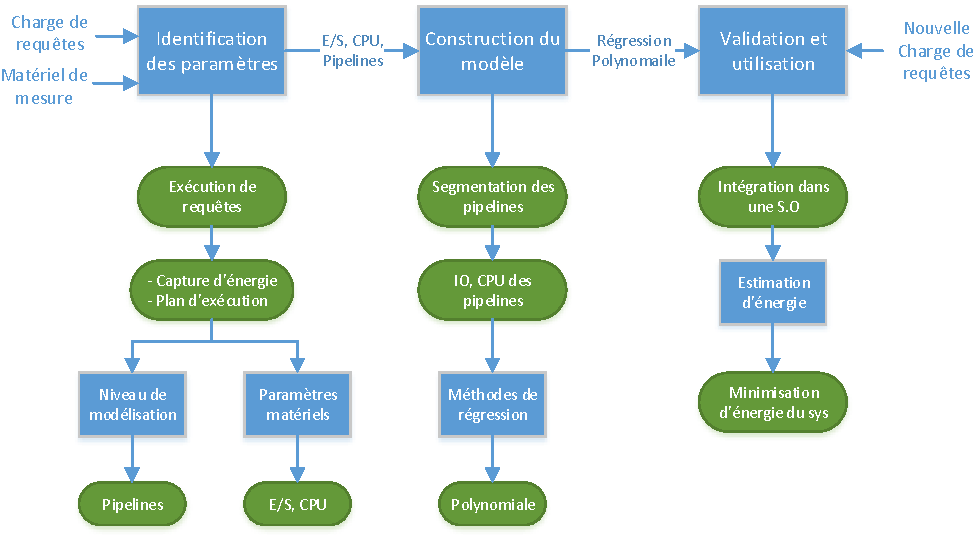
\includegraphics[scale=0.80]{chapitre4/chap4Fig/costmodel-methodology-final.pdf} % power-model.eps
 \caption{Vue d'ensemble sur le modèle de coût énergétique.}
 \label{fig:power-model}
\end{figure}

\section{Évaluation de notre modèle de coût}\label{sec:experiment}
Dans cette section, nous présentons des résultats expérimentaux montrant l'efficacité de notre modèle proposé. Nous décrivons d'abord l'architecture et le jeu de données d'expérimentations, puis nous évaluons la performance de notre modèle d'estimation d'énergie.

\subsection{Architecture d'expérimentations}
Pour mesurer la consommation réelle d'énergie, nous avons créé une configuration similaire aux travaux précédents \cite{Rodriguez11, Xu10b, Kunjir12} que nous utilisons même dans le reste de nos expérimentations présentées dans les prochains chapitres. Cette configuration utilise le multimètre << \textit{Watts UP? Pro ES} >> \footnote{https://www.wattsupmeters.com/} qui a une résolution maximale d'une seconde.
Le dispositif est directement connecté entre la prise d'alimentation et la station de travail sur laquelle la BD est déployée. Cet ordre permet de mesurer la consommation d'énergie globale de la station de travail. Les valeurs mesurées sont enregistrées et traitées dans une machine de contrôle séparée connectée avec le multimètre via un câble USB.
% \begin{figure}
%  \centering
%  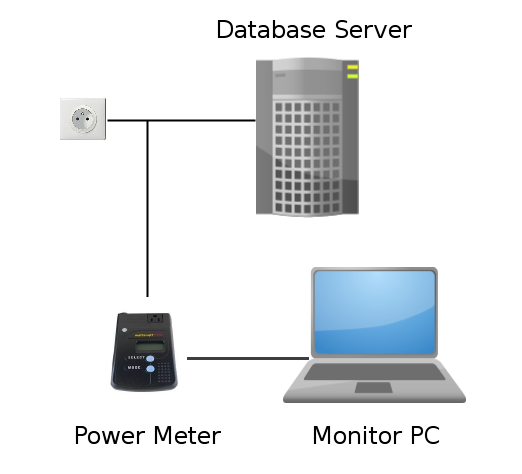
\includegraphics[scale=0.6]{chapitre4/chap4Fig/schema.png}
%  \caption{Architecture d'expérimentations.}
%  \label{fig:arch-setup}
% \end{figure}

Nous avons utilisé une station de travail Dell PowerEdge R210 II ayant un processeur Intel Xeon E3-1230 V2 de 3.30GHz, 10 Go de mémoire DDR3 et une configuration disque dur de 2x500 Go. A noter que des techniques comme la \textit{tension-fréquence dynamique du processeur} (DVFS) ne sont pas appliquées dans nos expérimentations. Nous répétons chaque expérience plusieurs fois pour assurer la confiance dans les valeurs observées.

Notre station de travail est installée avec la dernière version du SGBD Oracle 11gR2 sous Ubuntu Server 14.04 LTS avec noyau Linux 3.13. Afin de minimiser les influences indésirables, nous avons désactivé les tâches de fond inutiles et vidé le cache du système et le buffer d'Oracle avant chaque exécution de requête.

\subsubsection{Exécution des requêtes et capture d'énergie}

\begin{figure}
 \centering
 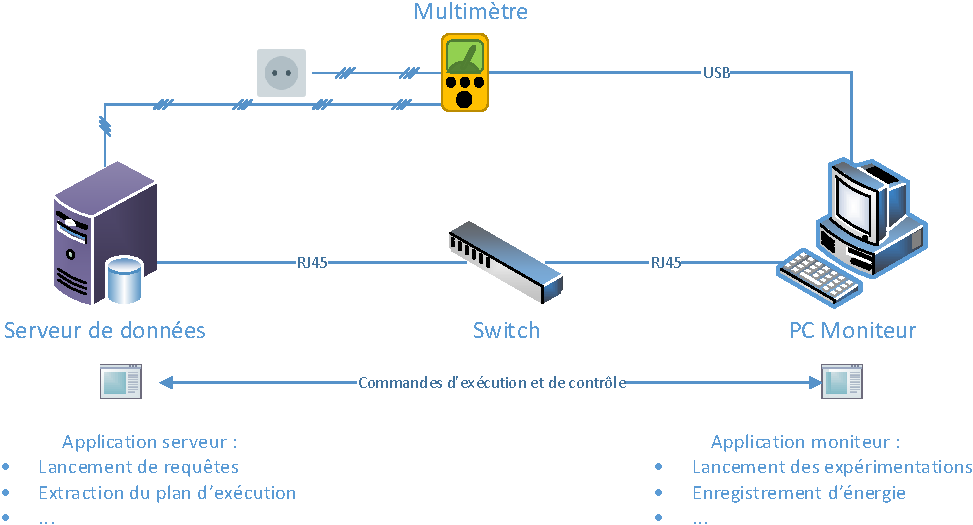
\includegraphics[scale=0.7]{chapitre4/chap4Fig/experiment-setup.pdf}
 \caption{Applications de gestion d'expérimentations.}
 \label{fig:experiment-setup}
\end{figure}

Pour réaliser nos expérimentations, nous avons développé une application et un script pour automatiser le processus des tests. La \ref{fig:experiment-setup} représente l'architecture logicielle des expérimentations. Une application client/serveur basée sur les sockets et implémentée en langage C est mise en œuvre. La machine de contrôle contient la partie serveur de l'application dont les tâches se résument à :
\begin{enumerate}
 \item l'établissement d'une connexion via le réseau avec la station de travail ;
 \item le lancement/l'arrêt des expérimentations ;
 \item l'enregistrement des valeurs d'énergie via le multimètre en invoquant son pilote.
\end{enumerate}

La station de travail contient la partie client de l'application  et ses tâches consistent à :
\begin{enumerate}
 \item l'établissement de la connexion avec l'application serveur ;
 \item le vidage du cache de la BD à l'aide des commandes Oracle suivantes:
 \begin{lstlisting}[language=sql]
-- Clean the cache
ALTER SYSTEM FLUSH SHARED_POOL;
ALTER SYSTEM FLUSH BUFFER_CACHE;
\end{lstlisting}
 \item le vidage du cache du système d'exploitation à l'aide du script \textit{shell} suivant :
 \begin{lstlisting}[language=bash]
#!/bin/bash
# To free pagecache, dentries and inodes (linux kernel)
sync && echo 3 | tee /proc/sys/vm/drop_caches
\end{lstlisting}
 \item la connexion avec le SGBD ;
 \item le lancement et la gestion d'ordonnancement de requêtes d'apprentissage et de tests ;
 \item l'extraction du plan d'exécution avec tous ses informations (coût d'E/S et de CPU, temps d'exécution des opérateurs, etc.), à l'aide de la commande Oracle suivante :
 \begin{lstlisting}[language=sql]
SELECT DBMS_SQLTUNE.report_sql_monitor(
  sql_id       => '526mvccm5nfy4',
  type         => 'ACTIVE',
  report_level => 'ALL') AS report
FROM dual;
\end{lstlisting}
\end{enumerate}

\subsection{Jeu de données}
Dans les expérimentations, nous utilisons les jeux de données et les requêtes issues des deux benchmarks TPC-H et TPC-DS \cite{TPCH, TPCDS}, interrogeant des données de 10 Go et de 100 Go de taille (facteur d'échelle). Le TPC-H est un benchmark décisionnel conçu pour le requêtage ad-hoc où les requêtes ne sont pas connues à l'avance. Le schéma modélise un modèle produits-commandes-fournisseurs contenant 2 tables de faits et 6 tables de dimensions (cf. \ref{fig:tpch-schema}), avec une charge de 22 requêtes décisionnelles caractérisées par un large volume de données et un degré élevé de complexité.
TPC-DS qui est le successeur annoncé de TPC-H, modélise un entrepôt de données. Le schéma de TPC-DS représente les fonctions décisionnelles d'un détaillant sous la forme de plusieurs schémas en flocon de neige. Il comprend 17 dimensions partagées par 7 tables de faits, ce qui le transforme en un schéma en constellation. Le \ref{tab:tpcds-table-rows} représente le nombre de lignes dans les tables de faits avec une taille de 100 Go (facteur d'échelle = 100). La charge de requêtes de TPC-DS est composée de 99 requêtes et  constituée de quatre classes de requêtes : requêtes de rapports, requêtes décisionnelles ad-hoc, requêtes de traitement analytique en ligne (On-Line Analytical Processing, OLAP) et requêtes d'exploration de données \cite{Nambiar06}.
\begin{figure}
 \centering
 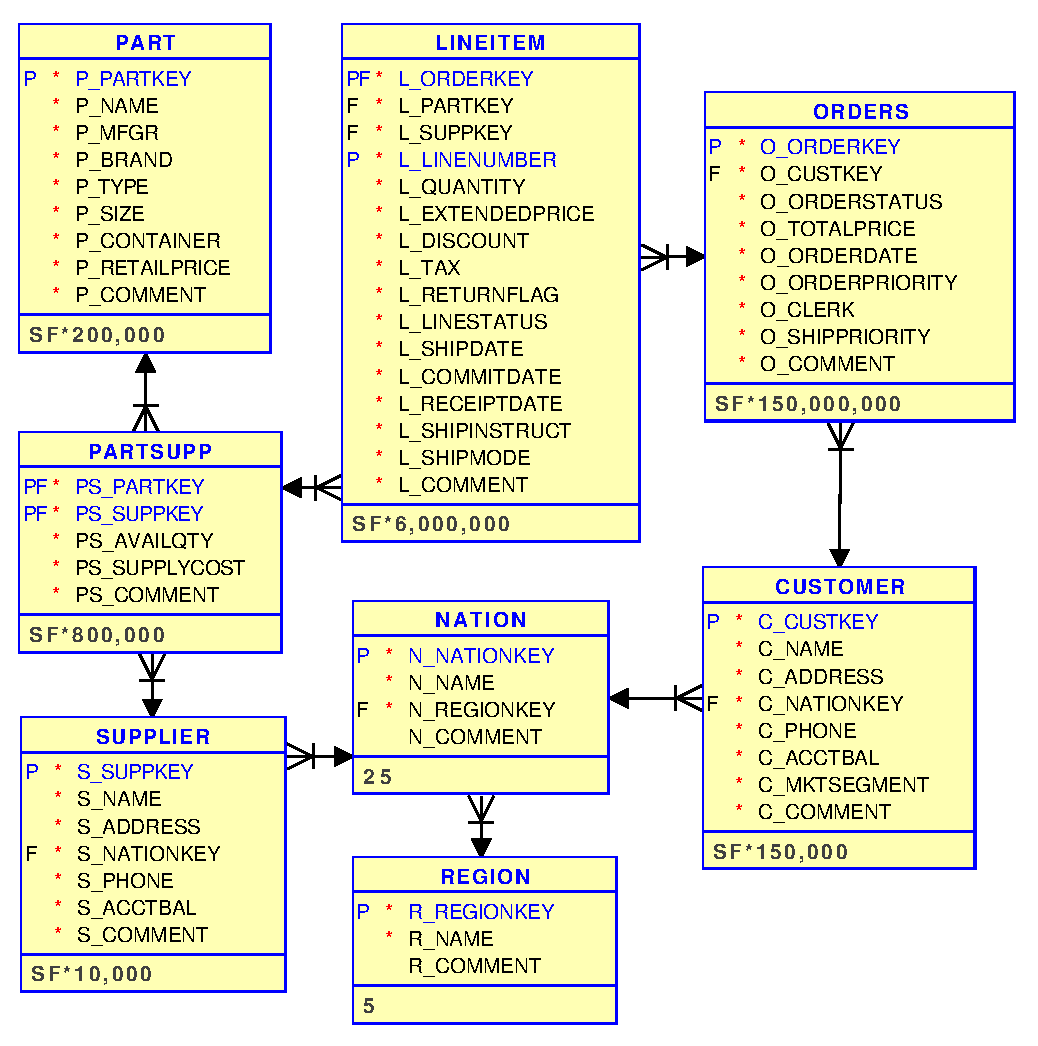
\includegraphics[scale=0.6]{chapitre4/chap4Fig/tpch-schema.pdf}
 \caption{Schéma du benchmark TPC-H.}
 \label{fig:tpch-schema}
\end{figure}

\begin{table}[]
\centering
\caption {Cardinalité des tables de faits du benchmark TPC-DS avec une taille de 100 Go.}\label{tab:tpcds-table-rows}
%\rowcolors{0}{}{lightgray}
\begin{tabular}{ll}
\toprule
\textbf{Table} & \textbf{Cardinalité} \\ \midrule
	store\_sales & 288 millions \\ 
	store\_returns & 28,8 millions \\ 
	catalog\_sales & 144 millions \\
	catalog\_returns & 14,4 millions \\
	web\_sales & 72 millions \\
	web\_returns & 7,2 millions \\
	inventory & 400 millions \\ \bottomrule
\end{tabular}
\end{table}

L'ensemble des données et de requêtes des deux benchmarks ont été générés avec l'outil \texttt{dbgen} fourni par le TPC. Une fois les données générées, des scripts sont utilisés pour peupler la BD à l'aide du l'outil \texttt{sqlloader} fourni par Oracle.
Dans le cas d'exécution des requêtes en mode isolé, chaque charge contient une seule requête (une seule requête est en exécution par le SGBD à un instant donné).
Dans le cas du mode concurrent, nous avons varié le taux de multiprogrammation (MPL $\in \{2,\cdots,10,13,15\}$).

\subsection{Résultats pour une requête isolée}
Comme décrit dans la section précédente, notre modèle de coût est composé de deux parties : les paramètres d'énergie qui peuvent être calculés par le biais d'une procédure d'apprentissage, et les paramètres de pipeline (p. ex. les coûts CPU et E/S) qui peuvent être lus à partir des statistiques de BD déjà disponibles. Dans cette section, nous présentons les résultats de ces deux étapes.

\subsubsection{Résultat d'apprentissage}
Dans la phase d'apprentissage, nous collectons à chaque exécution de requête, des statistiques relatives à l'exécution des pipelines et à la consommation d'énergie du système. Ces données collectées sont utilisées par le logiciel R pour trouver les meilleures valeurs des paramètres du modèle. Sur la base des résultats obtenus, une preuve probabiliste pour démontrer les bornes de confiance de notre modèle et des résultats est donnée dans l'\ref{annex:ConfidenceBounds} (page \pageref{annex:ConfidenceBounds}).

Les résultats de la phase d'apprentissage pour les valeurs retournées par le modèle linéaire et polynomiale (l'\ref{eq:lin-reg-equation} et l'\ref{eq:poly-reg-equation}) sont tracés dans la \ref{fig:tpch-reg}.

\begin{figure}
  \centering
  \subfloat[Modèle de régression linéaire\label{fig:tpch-reg-lin}]{
    \centering
    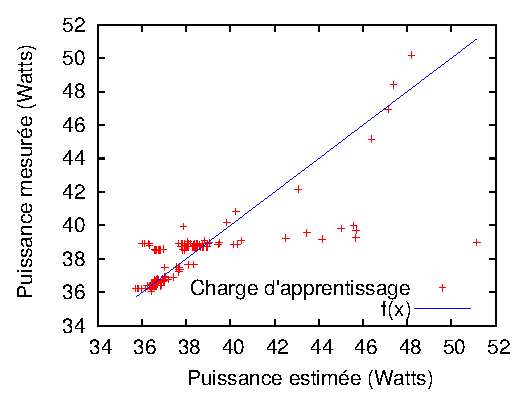
\includegraphics[width=0.45\textwidth]{chapitre4/chap4Fig/tpch-reg-lin.eps}
  }
  \quad
  \subfloat[Modèle de régression polynomiale\label{fig:tpch-reg-poly}]{
    \centering
    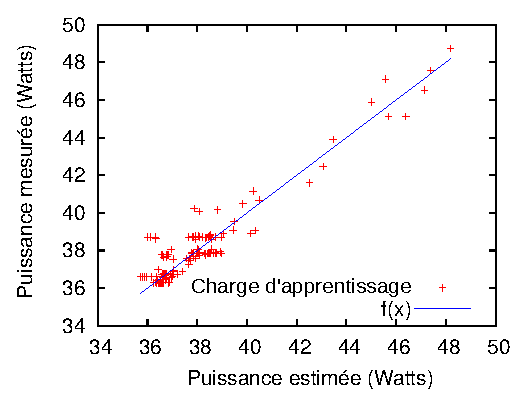
\includegraphics[width=0.45\textwidth]{chapitre4/chap4Fig/tpch-reg-poly.eps}
  }
  \caption{La qualité des méthodes de régressions pour la phase d'apprentissage du modèle de coût énergétique.}\label{fig:tpch-reg}
\end{figure}

Comme nous pouvons le voir sur la \ref{fig:tpch-reg-lin}, il existe des différences significatives entre la consommation d'énergie estimée et réelle pour de nombreuses requêtes. Néanmoins, la consommation d'énergie estimée et réelle rapprochent de près les lignes diagonales lors de l'utilisation d'une régression polynomiale (\ref{fig:tpch-reg-poly}).
% cela justifie notre choix d'utiliser une régression polynomiale

\subsubsection{Résultat avec TPC-H}
Pour tester notre modèle avec un grand ensemble de données, nous exécutons tous les 22 requêtes du benchmark TPC-H avec une taille de deux facteurs d'échelle, 10 Go et 100 Go. Nous notons que la plupart des requêtes contiennent plus de 4 pipelines.
Les résultats sont présentés dans le \ref{tab:tpch-results}.

\begin{table}[]
\centering
\caption {Erreurs d'estimation d'énergie dans les requêtes du benchmark TPC-H avec différentes tailles de BD.}\label{tab:tpch-results}
%\rowcolors{5}{}{lightgray}
\begin{tabular}{cccccc}
\toprule
\multirow{2}{*}{\textbf{Requête}} & \multicolumn{2}{c}{\textbf{Erreur (\%)}} & \multirow{2}{*}{\textbf{Requête}} & \multicolumn{2}{c}{\textbf{Erreur (\%)}} \\ \cmidrule(lr){2-3} \cmidrule(l){5-6} 
    & \textbf{10 Go} & \textbf{100 Go} & & \textbf{10 Go} & \textbf{100 Go} \\ \midrule
	$Q1$ & 1,2 & 0,9 & $Q12$ & 1,9 & 0,05 \\ 
	$Q2$ & 10,1 & 8,9 & $Q13$ & 12,8 & 6,1 \\ 
	$Q3$ & 1,0 & 0,1 & $Q14$ & 0,4 & 0,6 \\ 
	$Q4$ & 0,5 & 0,3 & $Q15$ & 2,3 & 1,0 \\ 
	$Q5$ & 1,2 & 0,6 & $Q16$ & 0,4 & 1,7 \\ 
	$Q6$ & 1,3 & 0,1 & $Q17$ & 0,2 & 1,4 \\ 
	$Q7$ & 1,1 & 0,7 & $Q18$ & 1,9 & 3,7 \\ 
	$Q8$ & 0,5 & 0,1 & $Q19$ & 0,6 & 1,0 \\ 
	$Q9$ & 1,9 & 0,8 & $Q20$ & 1,8 & 2,1 \\ 
	$Q10$ & 0,6 & 1,2 & $Q21$ & 0,9 & 0,4 \\ 
	$Q11$ & 4,8 & 0,3 & $Q22$ & 0,007 & 2,1 \\ \bottomrule
\end{tabular}
\end{table}

Comme nous pouvons le voir dans le tableau, l'erreur moyenne est généralement très minimale (1,6\% pour l'ensemble de données de 10 Go et 2,1\% pour celui de 100 Go), et l'erreur maximale est habituellement au-dessous de 5\%. Les plus grandes erreurs dans les estimations faites par notre modèle de coût (p. ex. \textit{Q2} et \textit{Q13}) sont dues à des erreurs d'estimation de cardinalité faite par l'optimiseur de requêtes.

Par exemple, le troisième pipeline de \textit{Q2} de l'ensemble de données de 100 Go est le plus long pipeline dans la requête. Le nombre estimé de lignes est de seulement 180 692 lignes tandis que le nombre réel de lignes est de 1 362 975. Ainsi, les valeurs des coûts de CPU et de E/S sont systématiquement fausses. Puisque notre étude dans ce stade traite les SGBD comme une << boîte noire >>, nous ne pouvons pas vérifier le modèle basé sur des cardinalités réelles qui sont obtenues après l'exécution de la requête.

\subsubsection{Résultat avec un schéma complexe : TPC-DS}
Pour vérifier la portabilité du modèle sur un nouveau schéma de BD, nous avons pris le benchmark TPC-DS qui est plus complexe que le benchmark TPC-H en raison de son schéma diverse, sa distribution de données et sa charge de requête d'aide à la décision. Nous avons utilisé une BD d'une taille de 100 Go.

Motivé par \cite{Poess07}, nous avons sélectionné 16 requêtes sur les 99 requêtes, en veillant à ce que les deux types soient présents (requêtes gourmandes en CPU et/ou en E/S). Le nombre moyen des pipelines est 7. La \ref{fig:tpcds-100-set1-power} montre les résultats d'expérimentation. On constate que l'erreur des prédictions du modèle est inférieure à 10\%. De même, nous observons la présence d'une seule requête avec une erreur importante, à savoir la \textit{Q47}. En analysant la structure de cette requête, nous avons constaté que l'erreur vient du fait que le coût de la fonction analytique \texttt{rank()} n'est pas donné par le SGBD. Pour le vérifier, nous avons supprimé la partie de code SQL contenant la fonction \texttt{rank()} dans \textit{Q47} et nous l'avons renommée et exécutée sous le nom de \textit{Q47p}. Comme nous pouvons le voir dans la \ref{fig:tpcds-100-set1-power}, l'erreur d'estimation est descendue à 7,5\%.

Cette situation (calcul du coût des agrégations et des fonctions d'analyse) doit être considérée par les vendeurs de SGBD pour faciliter le développement de BD énergétique, comme précédemment souligné dans \cite{Harizopoulos09, Graefe08}.

\begin{figure}
 \centering
 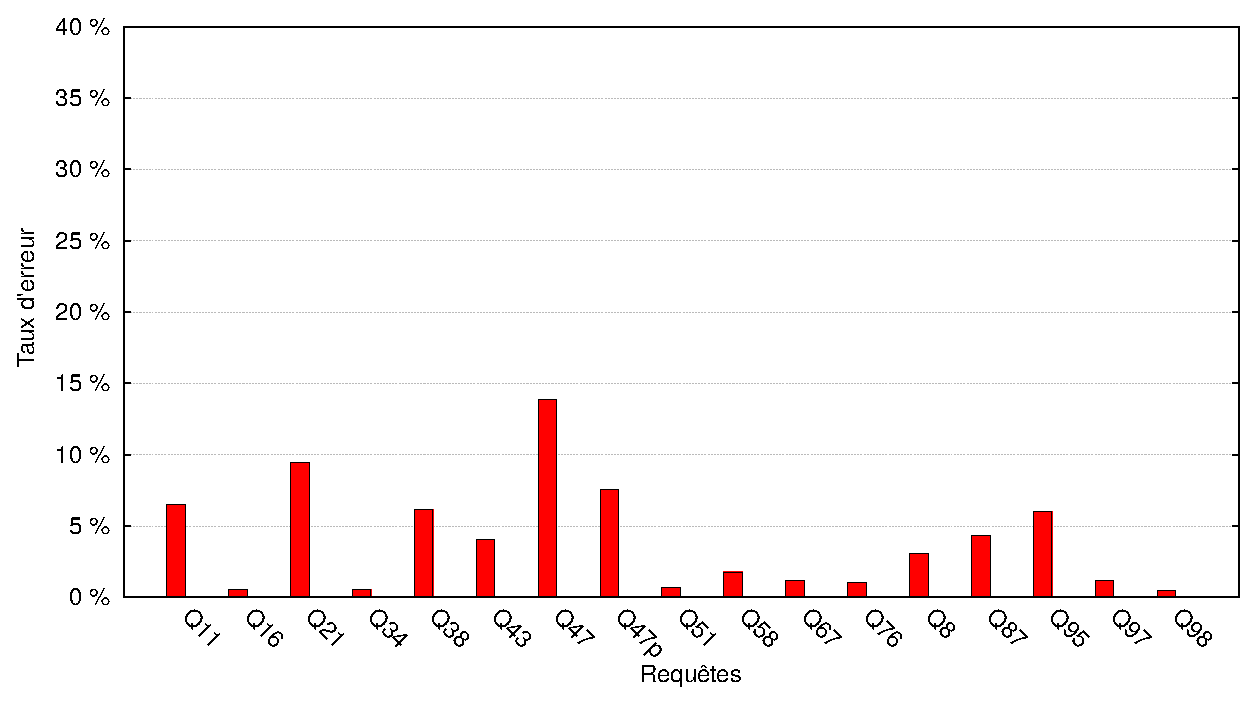
\includegraphics[scale=0.5]{chapitre4/chap4Fig/tpcds-100-set1-error.eps}
 \caption{Erreurs d'estimation d'énergie dans les requêtes du benchmark TPC-DS.}
 \label{fig:tpcds-100-set1-power}
\end{figure}

\subsubsection{Résultat avec une nouvelle configuration matérielle}
Dans un autre test, nous avons réduit la mémoire de BD à 2 Go et exécuté la charge de requêtes du TPC-H. Les résultats sont présentés dans le \ref{tab:tpch-2ram-results}.
Dans ce scénario, lorsque les résultats intermédiaires des opérateurs (comme la phase de construction de la table de hachage ou de tri externe) ne peuvent pas tenir dans la mémoire disponible, le SGBD va les enregistrer sur le disque. Cela conduit à plus d'E/S et un changement de comportement de consommation d'énergie. L'expérience montre que l'erreur d'estimation moyenne est de 2,5\%. Ainsi, notre modèle peut faire face à cette situation.

\begin{table}[]
\centering
\caption {Erreurs d'estimation d'énergie dans les requêtes du benchmark TPC-H avec 2 Go de mémoire.}\label{tab:tpch-2ram-results}
%\rowcolors{0}{}{lightgray}
\begin{tabular}{cccc}
\toprule
\textbf{Requête} & \textbf{Erreur 10 Go (\%)} & \textbf{Requête} & \textbf{Erreur 10 Go (\%)} \\ \midrule
	$Q1$ & 1,4 & $Q12$ & 0,8 \\ 
	$Q2$ & 11,9 & $Q13$ & 4,2 \\ 
	$Q3$ & 1,4 & $Q14$ & 1,7 \\
	$Q4$ & 0,7 & $Q15$ & 1,9 \\
	$Q5$ & 2,4 & $Q16$ & 2,4 \\
	$Q6$ & 1,5 & $Q17$ & 0,8 \\ 
	$Q7$ & 2,7 & $Q18$ & 6,5 \\
	$Q8$ & 1,5 & $Q19$ & 0,0 \\ 
	$Q9$ & 2,2 & $Q20$ & 0,3 \\ 
	$Q10$ & 2,7 & $Q21$ & 2,3 \\
	$Q11$ & 5,6 & $Q22$ & 0,07 \\ \bottomrule
\end{tabular}
\end{table}

\subsubsection{Résultat avec un nouveau SGBD}
Dans ces expérimentations, nous avons à la fois changé le SGBD et le matériel de déploiement  pour voir la robustesse de notre modèle. Précisément, nous avons utilisé le SGBD libre PostgreSQL en version 9.4.5, et comme matériel, nous avons utilisé une station de travail Dell PowerEdge R310 ayant un processeur Xeon X3430 de 2,40 GHz et 32 Go de mémoire DDR3. Pour la BD, nous avons utilisé le même benchmark TPC-H avec un facteur d'échelle de 10 et de 100 Go.
Les résultats de l'exécution de la charge de requêtes sont présentés dans le \ref{tab:tpch-results-postgres}.
Nous notons que certaines requêtes ont été interrompues car elles dépassent les 72 heures d'exécution dans notre environnement de test.

\begin{table}[]
\centering
\caption {Erreurs d'estimation d'énergie pour les requêtes du benchmark TPC-H avec PostgreSQL.} \label{tab:tpch-results-postgres}
%\rowcolors{5}{}{lightgray}
\begin{tabular}{cccccc}
\toprule
\multirow{2}{*}{\textbf{Requête}} & \multicolumn{2}{c}{\textbf{Erreur (\%)}} & \multirow{2}{*}{\textbf{Requête}} & \multicolumn{2}{c}{\textbf{Erreur (\%)}} \\ \cmidrule(lr){2-3} \cmidrule(l){5-6} 
    & \textbf{10 Go} & \textbf{100 Go} & & \textbf{10 Go} & \textbf{100 Go} \\ \midrule
	$Q1$& 1,03 & 0,2 & $Q11$ & 4,2 & - \\
	$Q2$& - & - & $Q12$ & 0,9 & 0,02 \\
	$Q3$& 1,5 & 1,2 & $Q13$ & 4,7 & 4,4 \\ 
	$Q4$& 0,6 & 0,5 & $Q14$ & 2,8 & 2,4 \\ 
	$Q5$& 1,2 & 3,07 & $Q15$ & 0,4 & 2,7 \\ 
	$Q6$& 4,1 & 2,7 & $Q16$ & 5,4 & 0,03 \\ 
	$Q7$& 0,4 & 1,4 & $Q18$ & 0,4 & - \\ 
	$Q8$& 0,07 & 1,09 & $Q19$ & 1,6 & 0,9 \\ 
	$Q10$& 0,6 & 0,3 & $Q22$ & 1,2 & 0,4 \\
	\bottomrule
    \end{tabular}
\end{table}

Les résultats dans cette nouvelle configuration logicielle et matérielle sont aussi de bonne qualité, comme nous pouvons le voir dans le tableau. L'erreur moyenne est 0,1\% dans les deux ensembles de données (100 Go et 10 Go) et l'erreur maximale est au-dessous de 6\%. L'expérience montre la robustesse de notre modèle de coût, indiquant qu'il est suffisamment prêt pour être intégré dans les structures d'optimisation d'énergie.

\subsection{Résultats pour des requêtes concurrentes}
Dans cette section, nous présentons les résultats d'évaluation de notre modèle de coût énergétique dans le cas des requêtes exécutées en mode concurrent.

\subsubsection{Résultat d'apprentissage}
Dans la phase d'apprentissage, nous avons créé une charge de requêtes avec 12 modèles de requête issus du benchmark TPC-H. Plus précisément, les modèles que nous avons utilisés sont les requêtes : 1, 3, 4, 5, 9, 11, 14, 16, 18, 19, 21, et 22, avec le facteur d'échelle de 10 Go. Nous nous référons à cet ensemble comme l'ensemble des modèles \textit{connus}.
Pour chaque MPL, nous avons généré des mixes de requêtes contenant le même modèle de requête, mais avec différentes instances en utilisant des outils de TPC-H. Ceci résulte en 287 mixes de pipeline composés de 132 charges de requêtes.
%DONE composés de 132 charges de requêtes ou de 132 requetes ? it's different -> ME: oui charge de requetes
À chaque exécution d'un mix de requêtes, nous collectons les statistiques des pipelines et nous enregistrons la consommation d'énergie du système. Ces données sont utilisées par le logiciel R pour trouver les meilleures valeurs de nos paramètres du modèle.
Nous ne considérons pas de grandes tailles de données dans cette partie d'étude, car les requêtes prennent beaucoup de temps pour terminer leur exécution. Par exemple, un simple mix de cinq requêtes générées à partir du benchmark TPC-H avec une taille de 100 Go prend 3 heures pour terminer son exécution. Cela peut requérir des semaines d'apprentissage et de test pour notre modèle. En outre,  il est probable dans ce cas qu'un mix de requêtes pourrait compléter l'ensemble de leurs exécutions dans un mode isolé plus rapide que l'exécution dans un mode concurrent.

\begin{figure}
  \centering
  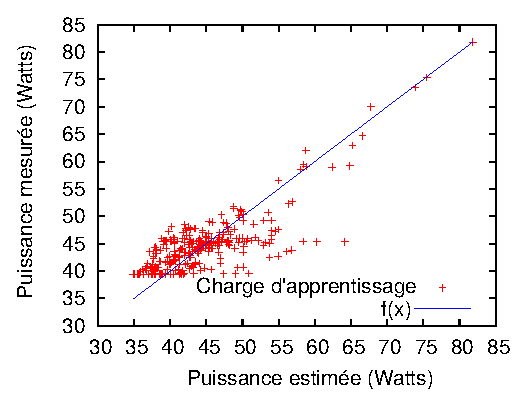
\includegraphics[width=0.5\textwidth]{chapitre4/chap4Fig/tpch-reg-poly-concurrent.eps}
  \caption{La qualité de la régression polynomiale pour la phase d'apprentissage du modèle de coût énergétique en mode concurrent.}\label{fig:tpch-reg-concurrent}
\end{figure}

Les résultats de la phase d'apprentissage comparés aux valeurs ajustées du modèle polynomial sont illustrés par la \ref{fig:tpch-reg-concurrent}. Comme nous pouvons voir sur la figure, la consommation d'énergie estimée et réelle rapprochent de près les lignes diagonales, indiquant ainsi la qualité de l'estimation que notre modèle peut générer. Il y a un certain écart entre l'estimation et l'énergie observée pour certains mixes de requêtes. Comme dans le cas du mode d'exécution isolé, une grande partie de ces erreurs est provoquée par l'optimiseur de requêtes, qui ne réussit pas à estimer les cardinalités de façon correcte lors de la phase de génération des plans d'exécution.

\subsubsection{Résultat avec des requêtes connues}
Pour évaluer notre modèle,  nous avons d'abord créé des charges de requêtes basées sur les modèles de requête TPC-H \textit{connus} d'une façon aléatoire. Pour chaque MPL, nous avons généré de nouveaux mixes à partir des 12 modèles, qui se traduit par 132 charges de requêtes.
%DONE idem que la previous todo 
Cependant, la génération aléatoire de mixes (échantillonnage) peut produire des mixes contenant les mêmes requêtes. Ainsi, cette technique ne couvre pas bien l'espace de mixes de requêtes possibles. Par conséquent, nous avons utilisé la méthode d'échantillonnage par hypercube latin (\gls{LHS}) \cite{Ahmad11}.
LHS crée un hypercube avec la même dimensionnalité que le nombre de modèles de requête \textit{T}. Chaque dimension est divisée en \textit{n} classes égales. La classe \textit{i} représente le nombre d'instances possibles du modèle de requête \textit{i}. LHS sélectionne alors \textit{n} mixes de l'espace de telle sorte que chaque classe de chaque modèle de requête apparaît dans exactement un mix. Intuitivement, LHS a une meilleure couverture de l'espace de mixes que la technique d'échantillonnage aléatoire.

\begin{figure}%[!ht]
  \centering
  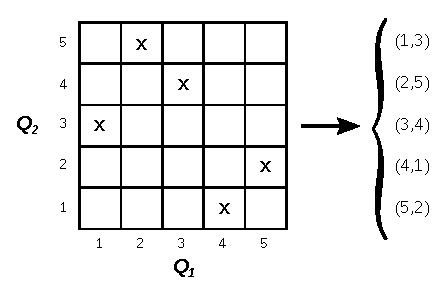
\includegraphics[width=0.5\textwidth]{chapitre4/chap4Fig/lhs.eps}
  \caption{Exemple d'échantillonnage par hypercube latin en 2-D.}\label{fig:lhs}
\end{figure}

La \ref{fig:lhs} montre un exemple où nous avons deux modèles de requête ($T = 2$), et nous devons sélectionner $n = 5$ mixes en utilisant LHS. Les deux axes $Q_1$ et $Q_2$ dans la figure désigne le nombre d'instances de requêtes de chaque type de requête dans un mix. La méthode d'échantillonnage par hypercube latin divise chacune de ces dimensions en 5 intervalles égaux. Les symboles << x >> désignent l'ensemble des mixes sélectionnés par la méthode LHS.

Nous avons testé la précision de la prédiction de notre modèle sur les mixes générés des modèles connus. La \ref{fig:tpch-test-all} montre les résultats des expérimentations.

\begin{figure}
 \centering
 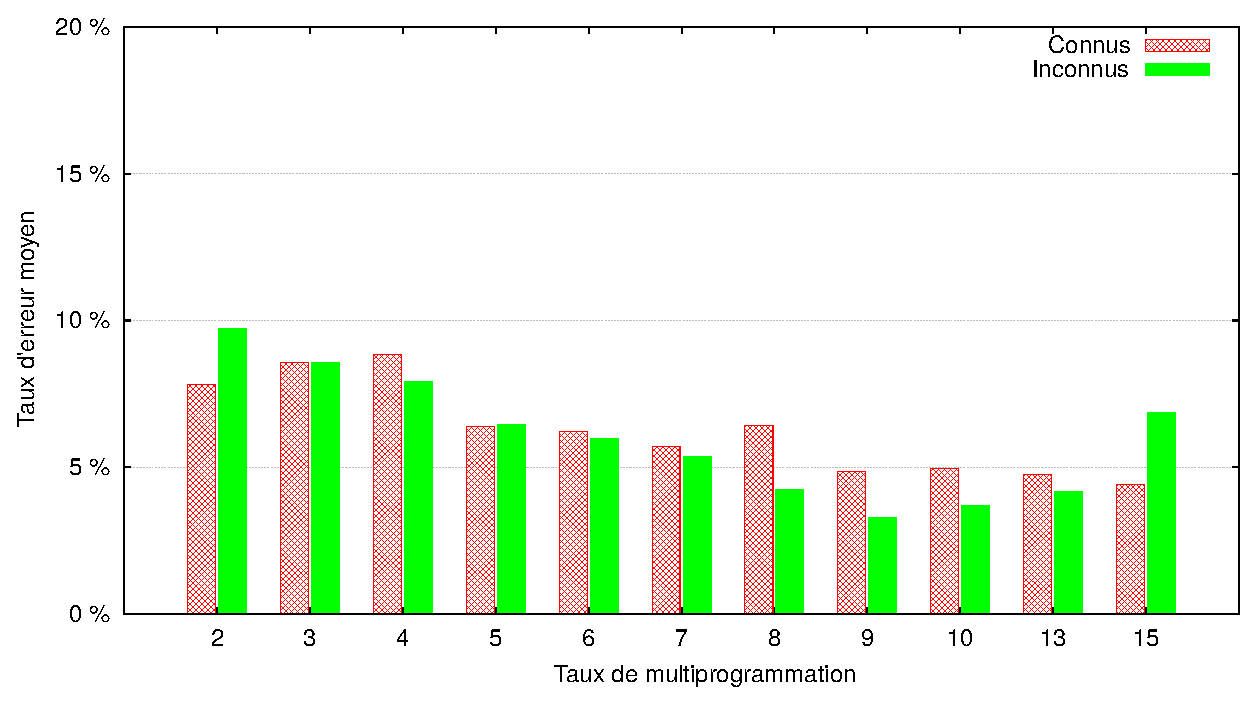
\includegraphics[scale=0.6]{chapitre4/chap4Fig/tpch-test-all.eps}
 \caption{Erreurs d'estimation d'énergie dans le benchmark TPC-H pour les modèles de requêtes connus et inconnus.}
 \label{fig:tpch-test-all}
\end{figure}

Comme illustré par la figure, l'erreur moyenne sur tous les est de 6,3\%  qui est considérée petite étant donné la variété de niveau de concurrence. En outre, l'erreur maximale est généralement inférieure à 9\%.

Notons en passant que nous pouvons voir que l'erreur est légèrement plus grande lorsque le MPL est petit (MPL = 2, 3 ou 4). Nous avons constaté que lorsque le MPL est élevé, la durée d'exécution des phases de pipeline est grande et notre modèle peut capturer leur consommation d'énergie. \`A l'inverse, lorsque le MPL est petit,  certaines phases de pipeline finissent leur exécution rapidement et notre modèle ne peut pas estimer leur consommation d'énergie avec précision. Ce problème est également observé dans certaines autres expérimentations.

\subsubsection{Résultat avec des requêtes inconnues}
Afin de tester notre modèle de coût contre de \textit{nouveaux} modèles de requêtes inconnues, nous avons créé des charges de requêtes basées sur le reste des requêtes du benchmark TPC-H qui ne sont pas utilisés dans la phase d'apprentissage, en utilisant la technique LHS. Plus précisément, pour chaque MPL nous avons généré 10 nouveaux mixes de requêtes, qui donnent lieu à 110 charges de requêtes.
%DONE idem, la je crois que cest vraiment charges de req :) -> ME: lol oui :)
 Les résultats sont présentés dans la \ref{fig:tpch-test-all}. On peut observer que les erreurs des prédictions du modèle de coût sont moins de 10\% pour les modèles de requêtes \textit{inconnus}, confirmant ainsi sa robustesse. %DONE a revoir ma reformulation

\subsubsection{Résultat avec un schéma complexe}
Pour vérifier la portabilité du modèle sur un nouveau schéma, nous avons choisi le schéma du benchmark TPC-DS. Nous nous sommes basés sur le même ensemble de 16 requêtes sélectionné dans le cas du mode d'exécution isolé. En utilisant la technique LHS, nous avons généré 16 mixes de requêtes pour chaque MPL, qui se traduit par 176 charges de requête. %DONE charges ou requetes :) je ne lache pas ;) -> ME: workload :)

La \ref{fig:tpcds-test-unknown} montre les résultats d'expérimentations. On peut observer que l'erreur des prédictions du modèle est inférieure à 10,5\%, ce qui montre que la modélisation de pipeline est un indicateur robuste pour la prédiction d'énergie dans le cas des données et des requêtes inconnues.

\begin{figure}
 \centering
 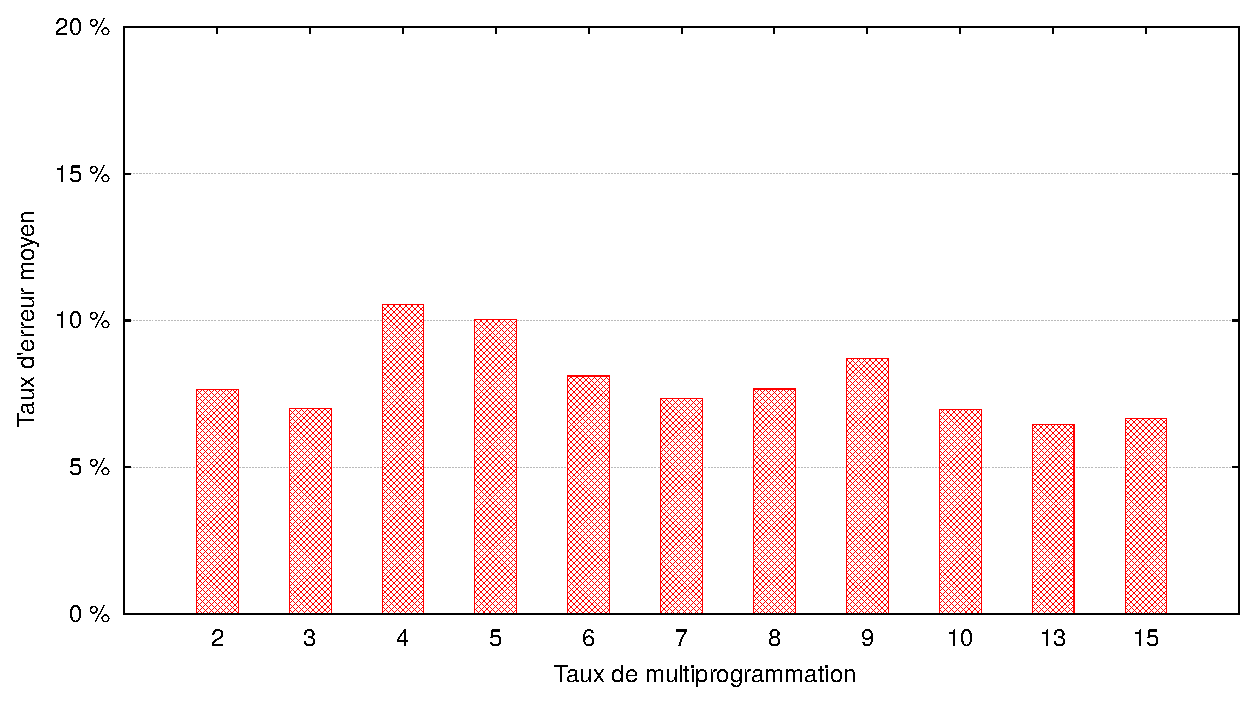
\includegraphics[scale=0.6]{chapitre4/chap4Fig/tpcds-test-unknown.eps}
 \caption{Erreurs d'estimation d'énergie dans les requêtes du benchmark TPC-DS en mode concurrent.}
 \label{fig:tpcds-test-unknown}
\end{figure}

\subsubsection{Résultat avec des charges de requêtes aléatoires}
Enfin, nous évaluons la précision de notre modèle pour prédire la consommation d'énergie pour tous les modèles de requête TPC-H de façon plus réaliste. Dans ces expérimentations et pour créer la charge de requêtes, nous passons par la liste de modèles de requêtes et nous ajoutons une instance de chaque modèle. En passant par la liste de modèles de nouveau d'une manière round-robin, nous continuons d'ajouter une instance de chaque modèle de requête à la charge jusqu'à ce que toutes les requêtes sont ajoutées. %TODO c'est moi qui s'est fatiguée ou je n'ai rien compris ?!! merci de revoir le paragraphe
En se basant sur les 22 requêtes de TPC-H, nous avons utilisé 4 instances pour chaque modèle de requêtes, ce qui résulte en une charge de 88 requêtes. Pour chaque MPL $M$, nous exécutons le premier mix de requête $M$, chaque fois qu'une requête se termine parmi les $M$ requêtes en cours d'exécution, une nouvelle requête à partir de la charge sera programmée à sa place sur la base de la politique d'ordonnancement First in, First out (FIFO). Cela nous donne une charge de requêtes d'une longue durée d'exécution qui prend en moyenne 2 heures pour terminer.

\begin{figure}
 \centering
 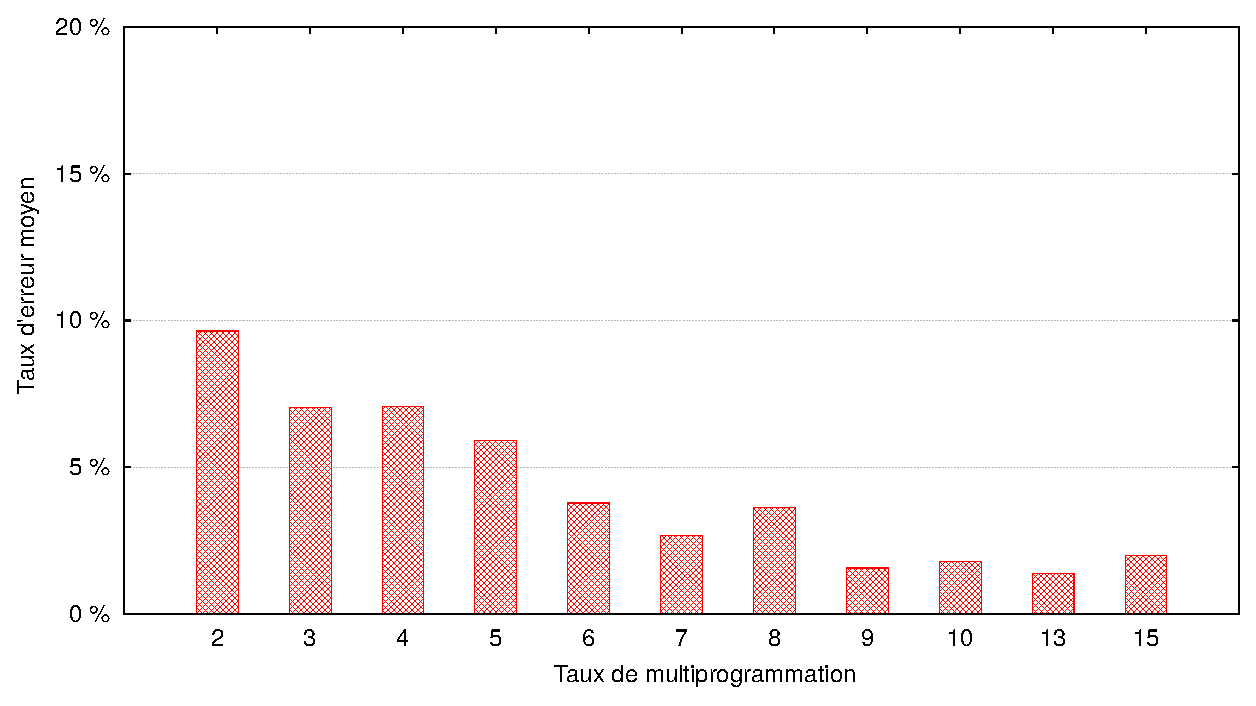
\includegraphics[scale=0.6]{chapitre4/chap4Fig/tpch-test-workload.eps}
 \caption{Erreurs d'estimation d'énergie dans le benchmark TPC-H pour tous les modèles de requêtes.}
 \label{fig:tpch-test-workload}
\end{figure}

Les résultats sont présentés dans la \ref{fig:tpch-test-workload}. Comme dans l'expérimentation précédente, les petits MPL  donnent des erreurs importantes par rapport aux grands MPL. Notre suggestion pour traiter ce scénario, est de modéliser l'énergie pour chaque groupe de MPL, par exemple, la création de modèle pour MPL $M1 \in \{2, \cdots, 5\}$, $M2 \in \{6, \cdots, 10\}$, $M3 \in \{11, \cdots, 15\}$ et ainsi de suite. Pour un futur travail, nous pouvons étendre notre framework avec une stratégie de regroupement similaire.
L'expérimentation montre que l'erreur d'estimation maximale est de 9,6\%. Ainsi, notre modèle peut faire face à des charges de requêtes réalistes.

\subsection{Bilan et discussion}
%TODO: add text
Les résultats expérimentaux ci-dessus indiquent clairement que notre modèle offre des résultats d'estimation d'énergie comparables à ceux donnés par les travaux connexes manipulant des modèles de requêtes connus exécutées en mode isolé \cite{Xu13, Kunjir12}. De plus, notre framework offre une amélioration significative par rapport aux techniques existantes, car il peut offrir une précision de prédiction similaire dans des scénarios plus complexes (à savoir des modèles de requêtes et des ensembles de données inconnus) et les requêtes exécutées en parallèle avec un taux de concurrence réaliste.

% Challenges and Limits

\section{Conclusion}
Dans nos jours, la consommation d'énergie des ordinateurs est devenue une préoccupation majeure pour l'industrie et la société. En conséquence, les chercheurs ont mis au point des techniques matérielles et logicielles pour assurer une efficacité énergétique.

Dans ce chapitre, nous proposons un modèle de coût basé sur les pipelines pour estimer la consommation d'énergie lors de l'exécution d'une requête SQL et un ensemble de requêtes exécutées simultanément.
Nous avons aussi indiqué comment la modélisation de pipeline pourrait être un indicateur robuste pour la prédiction d'énergie.
Le modèle de coût est construit sur la base des résultats empiriques obtenus à partir d'une charge de requêtes d'apprentissage qui a été soigneusement créée. Les paramètres matériels sont obtenues par un algorithme de régression polynomiale multiple.
En outre, nous avons effectué des tests sur notre modèle avec une BD réelle en exécutant un ensemble de requêtes, et avons comparé leurs coûts énergétiques avec ceux prédits par le modèle. Nos résultats montrent que le modèle, qui utilise uniquement des coûts de l'optimiseur en entrées, peut prédire l'énergie avec une petite erreur.

\chapter{Intégration de l'énergie dans le traitement de requêtes d'un SGBD relationnel}
\label{chap5}

\epigraph{<< Energy and persistence conquer all things. >>}{--- \textup{Benjamin Franklin}}

\NoChapterPrefix \NoChapterNumberInRef {\hypersetup{linkcolor=black} \minitoc}

%% numérotation des figures, des tables et des équations préfixé par le numéro de chapitre
\makeatletter
\renewcommand{\thefigure}{\ifnum \c@section>\z@ \thechapter.\fi
 \@arabic\c@figure}
\@addtoreset{figure}{chapter}
\makeatother

\makeatletter
\renewcommand{\thetable}{\ifnum \c@section>\z@ \thechapter.\fi
 \@arabic\c@table}
\@addtoreset{table}{chapter}
\makeatother

\makeatletter
\renewcommand{\theequation}{\ifnum \c@section>\z@ \thechapter.\fi
 \@arabic\c@equation}
\@addtoreset{equation}{chapter}
\makeatother
%%-----------------------------------------------------------------
%% Résumé
%%-----------------------------------------------------------------

%laisser une page ou deux pages vides, telle est la question !
%\EmptyNewPage
\newpage

%********************************************************************************
%********************************************************************************
\section{Introduction}
Dans les centres de données, la majorité des ressources de calculs et de stockage sont dédiées aux serveurs de bases de données, ce qui rond les SGBDs l'un des principaux consommateurs d'énergie. Cela est dû à la grande quantité de données interrogée par des requêtes complexes; exécutées quotidiennement par un SGBD.
La performance est l'objectif principal qui vient à l'esprit lorsque nous parlons des capacités des SGBDs. Ceci est particulièrement nécessaire pour les scénarios de traitement de requêtes transactionnelles en ligne (\acrshort[hyper=false]{OLTP}) où des centaines et des milliers de transactions comme la mise à jour ou l'insertion de nouveaux tuples dans une relation doivent être exécutées en temps réel. Au fil des années, le temps de traitement des requêtes complexes a diminué grâce à diverses améliorations apportées aux composants matériels et logiciels.

Comme déjà indiqué, les SGBDs existants se concentrent à la haute performance lors de la phase de traitement des requêtes, tout en ignorant généralement la consommation d'énergie. Cependant, des études récentes indiquent qu'une bonne performance n'est plus le seul critère de qualité pour un << bon >> SGBD. Selon le rapport Claremont sur la recherche pour les bases de données, un SGBD éco-énergétique deviendra l'un des principaux domaines de recherche à l'avenir \cite{Claremont08,Abadi16}.

Dans ce chapitre, nous proposons une méthodologie, soutenue par un outil appelé \textit{EnerQuery}, qui crée des bases de données tout en économisant l'énergie lors de la phase de traitement des requêtes. Pour montrer son efficacité, nous mettons en œuvre cette outil dans le module de traitement de requêtes du SGBD libre PostgreSQL. Un modèle mathématique de coût est utilisé pour estimer la consommation d'énergie. Les paramètres de ce dernier sont identifiés par une méthode d'apprentissage automatique. Nous avons mené des expériences intensives en utilisant nos modèles de coûts, et un outil de mesure dédié à calculer l'énergie, tout en basant sur des données de benchmark TPC-H, afin de montrer l’efficacité de nos propositions.

\section{Pourquoi le traitement des requêtes ?}\label{PourquoiOptimisationLogique}
Dans ce chapitre, nous nous concentrons sur le module de traitement de requêtes, qui fait partie des principales composantes d'un SGBD. Plusieurs travaux ont été élaborés dans le domaine de traitement des requêtes depuis le début des années 1970 pour les bases de données traditionnelles. Parmi ces travaux, divers algorithmes et systèmes ont été proposés, tels que le projet \textit{System-R}, dont les résultats ont été largement intégrées dans de nombreux optimiseurs commerciaux (voir \ref{chap2}).

Pour améliorer l'efficacité énergétique lors de l'exécution des requêtes, deux approches sont possibles : (1) nous pouvons soit réduire le temps d'exécution de la requête, (2) soit réduire l'énergie consommée. Le premier aspect a été étudié de manière exhaustive dans plusieurs travaux de littérature, ce qui a conduit au développement des SGBDs relationnels à hautes performances d'aujourd'hui. Le deuxième aspect a été ignoré dans la plupart des études antérieures, mais il est de plus en plus pris en compte dans les projets de recherche récents comme nous avons vu dans le \ref{chap3}.

La phase de traitement de requêtes est une tâche primordiale, car elle est au cœur d'un SGBD. Cette phase doit être exécutée constamment dans le cas des entreprises et des sites web. L'optimiseur de requêtes peut générer un grand nombre de plans d'exécution pour la même requête, ce qui donne de diverses choix de compromis entre les coûts de performance et d'énergie. De plus, un SGBD maintient des statistiques sur les données de la base dans le but d'un traitement efficace des requêtes. Ces informations peuvent être directement utilisées pour dériver le profil d'énergie des requêtes, et aider à la prise de décision liée à la minimisation d'énergie.

\section{Démarche d'intégration de l'énergie dans le traitement de requêtes}\label{Demarche}
Afin de concevoir un traitement de requêtes éco-énergétique, nous proposons tout d'abord un audit de chaque composant, dans le but de vérifier s'il est sensible à l'énergie ou non. Après cette vérification, nous présentons en détail notre méthodologie pour construire le module de traitement de requêtes.

\subsection{Un audit de traitement de requêtes}
Rappelons que le module de traitement de requête est responsable de l'exécution des requêtes suivant un ou plusieurs besoins non fonctionnels, tels que le temps de réponse. Le processus d'exécution d'une requête donnée passe généralement par quatre étapes principales: (i) l'analyse syntaxique, (ii) la réécriture, (iii) la planification et l'optimisation et (iv) l'exécution (cf. \ref{fig:postgres-query-optimizer}). Pour illustrer ces étapes, nous considérons comme une étude de cas le SGBD PostgreSQL\footnote{\url{https://www.postgresql.org/}}.

\begin{figure}
	\centering
	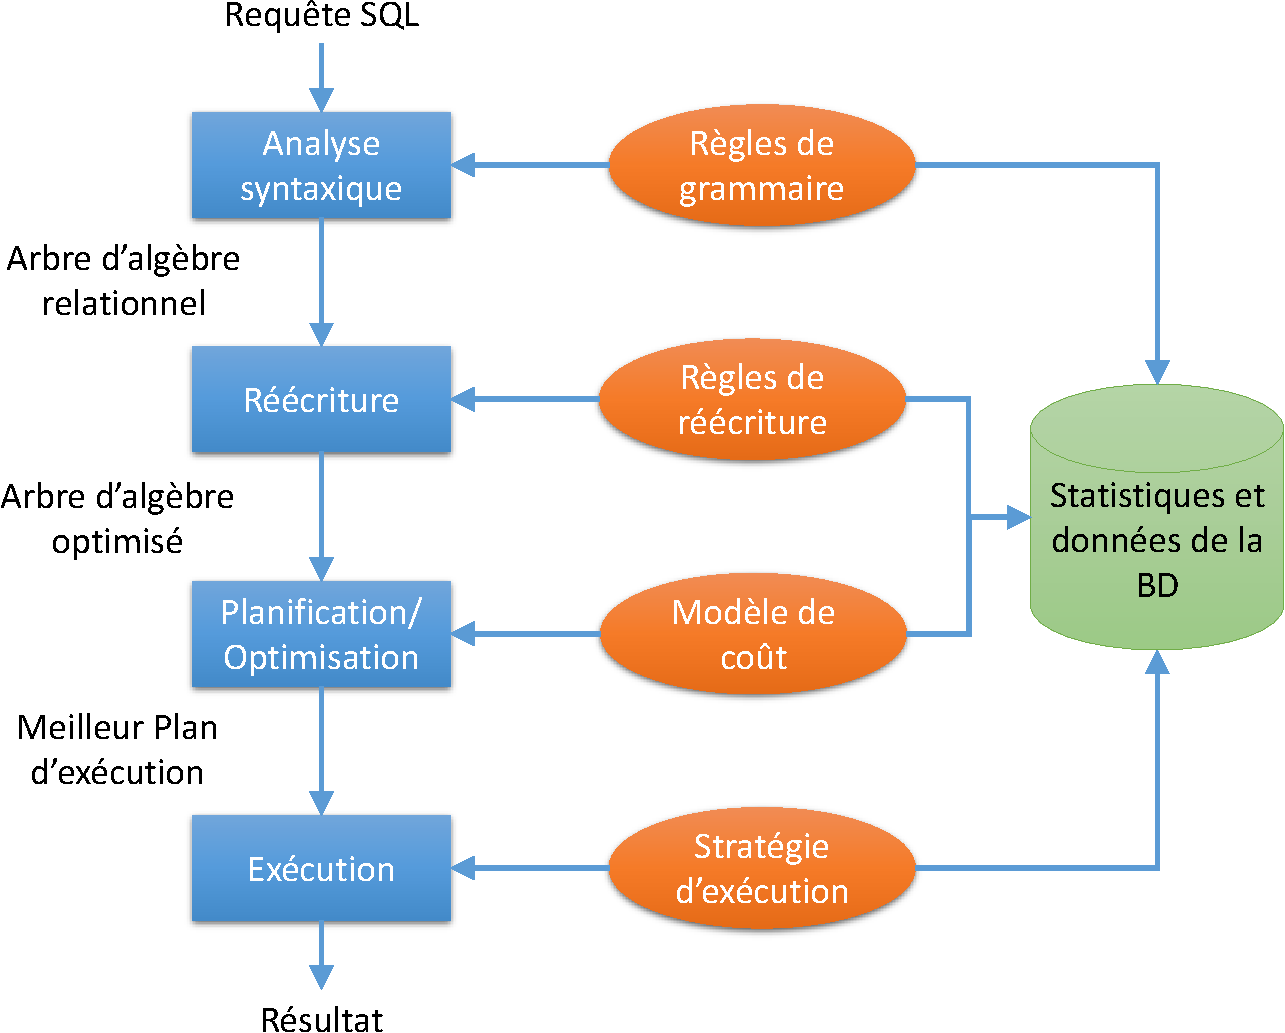
\includegraphics[scale=0.55]{chapitre5/chap5Fig/postgres-query-optimizer.pdf}
	\caption{Étapes de traitement de requêtes dans PostgreSQL.}
	\label{fig:postgres-query-optimizer}
\end{figure}

PostgreSQL est un système de gestion de base de données relationnelle et objet. C'est un outil libre et open-source développé à l'université de Californie à Berkeley par une équipe sous la direction de Michael Stonebraker en 1985. Le nom original était POSTGRES et fut renommé Postgres95. Ce dernier fut changé à la fin de 1996 en PostgreSQL. Il supporte diverses plates-formes matérielles et différents systèmes d'exploitation. PostgreSQL est entièrement conforme à ACID (atomicité, cohérence, isolation et durabilité), avec la prise en charge de nombreuses fonctionnalités comme les clés étrangères, jointures, vues matérialisées, triggers, récupération ponctuelle, tablespaces, réplication asynchrone, transactions imbriquées, sauvegardes en ligne, etc\footnote{\url{https://www.postgresql.org/docs/current/static/intro-whatis.html}}.

% add examples from PostgreSQL source code at each step
% Postgres:
% 2 Query planning in postgreSQL: Optimizing query execution to improve the energy efficiency of database management systems - Master
% Puissance-performance tradeoff in database systems - Master
% A3.pdf
\subsubsection{Analyse syntaxique}\label{subsec:Parse}
L'analyseur syntaxique doit vérifier la chaîne de caractères de la requête pour valider sa syntaxe à l'aide d'un ensemble de règles de grammaire.  Si la syntaxe est correcte, un \textit{arbre syntaxique} est construit et retourné. La fonction responsable de cette tâche dans PostgreSQL est : \texttt{raw\_parser()} située dans le fichier : \path{src/backend/parser/parser.c}. L'analyseur défini dans \texttt{gram.y} et \texttt{scan.l} est construit en utilisant les outils Unix \texttt{bison} et \texttt{flex}. Après la fin de la tâche d'analyseur, le processus de transformation prend l'arbre syntaxique en entrée et fait l'interprétation sémantique nécessaire pour comprendre quelles tables, fonctions et opérateurs référencés par la requête. La structure de données construite pour représenter cette information est appelée \textit{arbre de requête}. La fonction de transformation nommée \texttt{parse\_analyze()} est située dans le fichier \path{src/backend/parser/analyze.c}.  Le coût de cette phase est généralement ignoré par le SGBD car elle se termine très rapidement. Nous suivons la même logique et nous supposons que la consommation d'énergie de cette étape est négligeable.

\subsubsection{Réécriture}\label{subsec:Rewrite}
La phase de réécriture (ou simplification) des requêtes traite l'arbre remis par l'étape d'analyse syntaxique et le réécrit à un autre arbre en utilisant un ensemble de règles. Ces dernières sont définies par l'utilisateur ou le système. Cette phase basée sur des règles est également utilisée dans la réécriture des requêtes dans le cas des vues matérialisées. La fonction de réécriture est nommée \texttt{QueryRewrite()} définie dans le fichier \path{src/backend/rewrite/rewriteHandler.c}. Quant à l'étape précédente, le coût est ignoré en raison de l'achèvement rapide de cette phase.

\subsubsection{Planification/optimisation}\label{subsec:PlanOptimize}
La tâche du planificateur/optimiseur est de créer un plan d'exécution optimal. Une requête SQL donnée peut effectivement être exécutée de différentes manières, dont chacune va produire le même ensemble de résultats. La tâche de l'optimiseur est d'estimer le coût de l'exécution de chaque plan en utilisant une approche basée sur les coûts, et de trouver celle qui doit être exécutée rapidement.

\paragraph{Planification}
Le planificateur commence par générer des plans d'exécution pour la lecture de chaque relation individuelle (table) utilisée dans la requête. Les plans possibles sont déterminés par les \textit{indexes} disponibles sur chaque relation. Il y a toujours la possibilité d'effectuer un \textit{accès séquentiel} sur une relation, donc un plan de accès séquentiel est toujours créé. Si la requête nécessite la jointure de deux ou plusieurs relations, tous les plans possibles pour joindre ces relations sont générés. Les stratégies de jointure disponibles dans PostgreSQL sont: \textit {jointure par boucle imbriquée}, \textit{jointure par fusion} et \textit{jointure par hachage}. Lorsque la requête implique plus de deux relations, le résultat final doit être construit par un arbre de jointures, chacune avec deux entrées. Le planificateur examine les différentes séquences de jointure possibles pour trouver le moins cher en terme de coût. Si la requête utilise un nombre de relations moins d'un certain seuil défini (fixé à 12 relations dans PostgreSQL), une recherche quasi-exhaustive est effectuée pour trouver les meilleures séquences de jointure; autrement, un algorithme heuristique à base de génétique est utilisé.

Pour étudier les effets de ces stratégies de recherche, considérons la requête \textit{Q8} du benchmark TPC-H \cite{TPCH}. C'est une requête complexe qui implique la jointure de 7 tables. Nous modifions le planificateur de PostgreSQL selon trois manières : (i) la recherche d'un plan d'exécution en utilisant la stratégie du SGBD actuelle (ii) en utilisant l'algorithme génétique, et (iii) manuellement en forçant le planificateur de choisir un certain plan. Pour chaque stratégie, nous calculons son temps d'exécution et sa consommation totale d'énergie lors de l'exécution de la requête sur une base de données d'une taille de 10 Go. Les résultats sont présentés dans le \ref{tab:plan-algo}.

\begin{table}
\centering
\caption {Planification de la requête \textit{Q8} de TPC-H avec différentes stratégies de recherche.} \label{tab:plan-algo}
\begin{tabular}{lll}
    \toprule
    \textbf{Stratégie de recherche} & \textbf{Temps de planification (s)} & \textbf{Énergie (J)} \\
    \midrule
    Par défaut & 0,110006 & 5200,362\\ 
	Algorithme génétique & 0,977013 & 5387,648 \\ 
    Manuelle & 0,092054 & 5160,036 \\
    \bottomrule
\end{tabular}
\end{table}

D'après le tableau, on peut constater que la stratégie de choix d'un plan de requête manuel donne les meilleurs résultats, en terme de temps et d'énergie. Alors que la stratégie de recherche par défaut (semi-exhaustive) conduit à un temps d'exécution et de consommation d'énergie un peu plus élevée. L'algorithme génétique donne les pires résultats dans cet exemple, peut-être en raison du petit nombre de tables présent dans la requête, puisque cette stratégie est utilisée par le SGBD où il y a plus de 12 tables. Compte tenu de ce petit nombre de tables, si nous allons dans les bases de données opérationnelles réelles où il y a une centaine de tables, la stratégie de recherche utilisé par le planificateur peut conduire à une consommation d'énergie notable. Ainsi, la stratégie de recherche des plans d'exécution de requêtes manuellement par l'administrateur de base de données est recommandée dans les grandes bases de données pour gagner en efficacité énergétique.

\paragraph{Optimisation}
Pour évaluer le temps de réponse pour chaque plan d'exécution, des fonctions de coût sont définis pour chaque opérateur SQL basique. La formule générale pour estimer le coût de l'opérateur $op$ peut être exprimée comme:
\begin{equation}
 Co\hat{u}t_{op} = \alpha \times E/S \: \oplus \: \beta \times CPU \: \oplus \: \gamma \times Com
\end{equation} 
Où $E/S$, $CPU$ et $Com$ sont des estimations pour le nombres de pages, nombres de tuples et de messages de communication, respectivement, nécessaires pour exécuter l'opérateur $op$. Ils sont généralement calculés à l'aide des statistiques de base de données et des formules de sélectivité. Les coefficients $\alpha$, $\beta$ et $\gamma$ sont utilisés pour convertir les estimations à l'unité souhaitée (par exemple, le temps, l'énergie, etc). $\oplus$ représente la relation entre les paramètres (linéaires, non-linéaires).

L'optimiseur de PostgreSQL utilise cinq types de paramètres dans son modèle de coût, $T \in \{s, r, t, i, o\}$. Le coût d'un opérateur $op$ dans le plan de requête est calculé comme suit :
\begin{equation}
 Co\hat{u}t_{op} = \sum_{i=1}^{T} c_{i} \times n_{i}
\end{equation} 
Où $n$ représente l'estimation de coût d'opérations de type $T$ requises pour exécuter l'opérateur, et $c$ est le coefficient de coût de performance pour le même type. Les fonctions de calcul des coûts d'un opérateur seront représentées dans la \ref{sec:cost-model-param}. Le \ref{tab:postgres-cost-param} donne un aperçu des types d'opérateur définis dans PostgreSQL et les valeurs par défaut des coefficients de coût de performance. Le coût total estimé d'une requête est donc la somme des coûts des opérateurs individuels dans le plan d'exécution.

\begin{table}
\centering
\caption {Présentation des paramètres de modèle de coût de PostgreSQL.} \label{tab:postgres-cost-param}
\begin{tabular}{llll}
    \toprule
    \textbf{\textit{T}} & \textbf{Désignation} & \textbf{Définition} & \textbf{\textit{c}} \\
    \midrule
    $s$ & seq\_page\_cost        & le coût d'E/S pour accéder séquentiellement à une page  & 1,0 \\
    $r$ & random\_page\_cost     & le coût d'E/S pour accéder aléatoirement à une page     & 4,0 \\
    $t$ & cpu\_tuple\_cost       & le coût CPU pour traiter un tuple                       & 0,01 \\
    $i$ & cpu\_index\_tuple\_cost & le coût CPU pour traiter un tuple via un accès index    & 0,005 \\
    $o$ & cpu\_operator\_cost    & le coût CPU pour effectuer une opération (ex : hachage) & 0,0025 \\
    \bottomrule
\end{tabular}
\end{table}

Les paramètres des coefficients et leur relation peuvent être obtenus en utilisant diverses techniques telles que la calibration, la régression et les statistiques. Ainsi, un modèle de coût d'énergie doit être défini à ce niveau, avec les nouveaux paramètres $T$ les plus pertinents.

L'arbre du plan d'exécution final est constitué des opérations d'accès séquentiels ou d'accès par index des relations de base, plus des opérations de jointure par boucle imbriquée, fusion ou hachage, ainsi que des étapes auxiliaires, tels que les opérations de tri ou d'agrégation.

\subsubsection{Exécution}\label{subsec:Executor}
L'exécuteur prend le plan créé par le planificateur/optimiseur et le traite récursivement pour extraire l'ensemble de tuples requis dans un mécanisme de \textit{pipeline}. Chaque fois qu'un nœud du plan est appelé, il doit livrer le prochain tuple, ou signaler qu'il n'y a plus de tuples à livrer. Les requêtes complexes peuvent impliquer de nombreux niveaux de nœuds dans leurs plan d'exécution, mais l'approche générale reste la même : chaque nœud calcule et retourne sa prochaine sortie de tuple, à chaque fois qu'il est appelé. Chaque nœud est également responsable de l'application des expressions de sélection ou de projection qui ont été attribuées par le planificateur.

Pour étudier l'effet de l'étape d'exécution sur l'éco-conception d'un optimiseur de requêtes, nous considérons un exemple de requête \textit{Q22} issue du benchmark TPC-H.
La \ref{fig:q22-plan-pl} présente le plan d'exécution renvoyé par l'optimiseur de requête de PostgreSQL. Comme nous l'avons montré dans le \ref{chap4}, la consommation d'énergie est directement influencée par le modèle d'exécution du SGBD. Par conséquent, le plan d'exécution peut être divisé en un ensemble de segments, nous nous référons à ces segments comme \textit{pipelines}. Ces dernières correspondant à l'exécution simultanée d'une séquence contiguë d'opérateurs.
La segmentation du pipeline du plan d'optimiseur pour la requête \textit{Q22} est représentée sur la \ref{fig:q22-plan-pl}. Dans cette dernière, il y a 4 pipelines, et l'ordre d'exécution de ces pipelines est géré par les opérateurs de blocage (par exemple, PL3 ne peut débuter jusqu'à ce que PL2 se termine).

Dans notre étude précédente (cf. \ref{chap4}), nous avons montré que \textit{lorsqu'une requête passe d'un pipeline à l'autre, sa consommation d'énergie change aussi}. Lors de l'exécution d'un pipeline, la consommation d'énergie a généralement tendance à être constante. Par conséquent, ce modèle d'exécution de pipeline est très important, car il a un impact direct sur la consommation d'énergie lors de l'exécution d'une requête. L'éco-conception d'un optimiseur de requête devrait prendre en considération la stratégie d'exécution. Cet aspect n'est pas pris en charge dans les travaux de Xu \textit{et al.} \cite{Xu10b}.

\begin{figure}
	\centering
	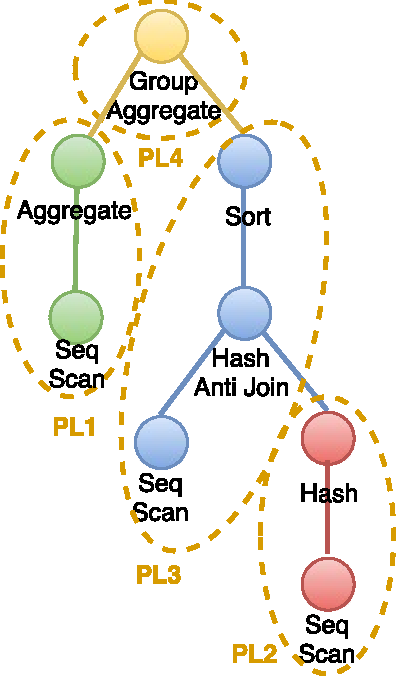
\includegraphics[scale=0.6]{chapitre5/chap5Fig/q22-plan-pl.pdf}
	\caption{Plan d'exécution du requête \textit{Q22} issue du benchmark TPC-H avec l'annotation de pipeline correspondante.}
	\label{fig:q22-plan-pl}
\end{figure}

\section{Méthodologie de conception d'un module de traitement de requêtes éco-énergétique}\label{sec:Methodology}

Dans cette section, nous décrivons la méthodologie de conception et la mise en œuvre de notre proposition dans le SGBD PostgreSQL. Comme nous l'avons mentionné ci-dessus, les phases de planification/optimisation et d'exécution ont un impact sur la consommation d'énergie, et doivent être prises en compte dans la conception d'un module de traitement de requêtes éco-énergétique. Le workflow de notre méthodologie est décrit dans la \ref{fig:methodo-postgres}. Nous avons étendu le module de traitement de requêtes de PostgreSQL pour inclure un modèle de coût estimant l'énergie des opérateurs SQL. Nous avons aussi modifié le processus de sélection des plans d’exécution \textit{mono-objectif} en un processus \textit{multi-objectifs} tout en incluant la dimension énergétique. Notre démarche ne génère pas de frais généraux au processus de traitement de requêtes car nous avons implémenté notre modèle énergétique à côté du modèle de performance existant, pour ne pas refaire les calculs pour chaque opérateur.

\begin{figure}
	\centering
	\includegraphics[scale=0.55]{chapitre5/chap5Fig/dbms-flow.pdf}
	\caption{La méthodologie de conception}
	\label{fig:methodo-postgres}
\end{figure}

\subsection{Modèle de coût d'énergie}
Dans cette section, nous présentons notre méthodologie pour l'estimation de la consommation d'énergie des requêtes dans PostgreSQL. Nous nous sommes basé sur notre démarche introduite dans le \ref{chap4} pour construire notre modèle. Les caractéristiques de ce modèle comprennent: (i) la segmentation d'un plan d'exécution en un ensemble de pipelines, (ii) l'utilisation des paramètres de pipeline pour construire le modèle en utilisant des techniques d'apprentissage automatique (\textit{hors ligne}), et (iii) l'estimation de l'énergie du nouveau pipeline en se basant sur le modèle de coût final (\textit{en ligne}). Les fonctions de régression et de calibration sont les mêmes que celles utilisées dans le \ref{chap4}.

%\subsubsection{Segmentation des pipelines}
\subsubsection{Paramètres du modèle de coût}\label{sec:cost-model-param}
Étant donné une requête SQL, l'optimiseur de requête est responsable de l'estimation des coûts d'E/S et de CPU pour chaque opérateur algébrique de base. Notre stratégie pour la modélisation d'énergie est d'étendre le modèle de coût de ces opérateurs qui sont intégrés dans le SGBD PostgreSQL, afin d'estimer sa consommation d'énergie.
Pour chaque opérateur, les paramètres dans l'\ref{eq:cost-model} (les coûts d'E/S et de CPU) doivent être modifiés en fonction de son implémentation et comportement d'exécution. La suite de cette section sera consacrée à présenter des modèles d'énergie pour un ensemble d'opérateurs relationnels de base.

\paragraph{Accès séquentiel} L'opération d'accès séquentiel parcourt la relation complète telle qu’elle est stockée sur disque, puisque chaque page et tuple doivent être examinés. Le coût d'E/S est égal au nombre de pages dans la relation ($p$), et le coût CPU est égal au nombre de tuples ($t$).
\paragraph{Accès par index} L'opération d'accès par index réalise un parcours d'un arbre d'index, passe à travers des nœuds feuilles pour trouver toutes les entrées correspondantes, et récupère les données correspondantes de la table. Pour chaque index, le nombre de tuples est déterminé par la fraction de tuples dans une relation qui satisfait les clauses de restriction. Cette quantité fractionnaire est appelée << sélectivité >> ($f$).
\paragraph{Accès par bitmap} Un accès par bitmap récupère tous les pointeurs de ligne dans l’index en une seule fois, les trie en mémoire en utilisant une structure bitmap, puis visite les lignes dans la table en suivant l’ordre de leur emplacement physique. Puisque l'accès par bitmap est basé sur l'accès par index, ses coûts d'E/S et de CPU sont calculés de la même façon.
\paragraph{Jointure par boucle imbriquée} La jointure par boucle imbriquée joint deux tables en récupérant le résultat d’une table ($inner$), et en recherchant chaque ligne de la première table dans la seconde ($outer$). Pour toutes les stratégies de jointure, l'estimation de la taille des deux relations $inner$ et $outer$ est obtenue par la multiplication de la taille originale de la relation par la sélectivité $f$ de chaque clause de restriction dans la jointure. Le coût d'E/S dans ce type de jointure est la somme du coût de la relation $inner$ et $outer$, le coût CPU est la multiplication de nombres de tuples dans chaque relation.
\paragraph{Jointure par tri-fusion} La jointure par tri-fusion combine deux listes triées comme une fermeture éclair. Les deux côtés de la jointure doivent être triés par les prédicats de jointure. Le coût d'E/S est la somme des coûts de la relation $inner$ et $outer$. Le coût CPU est égal à la somme des coûts pour trier les tuples des deux relations.
\paragraph{Jointure par hachage} La jointure de hachage charge les tuples candidats d’un côté de la jointure dans une table de hachage dont chaque enregistrement est ensuite testé avec l’autre côté de la jointure. Le coût d'E/S est le coût de lecture des deux relations $outer$ et $inner$, et le coût CPU est égal à la somme des coûts dans la phase de construction de la table de hachage $n_hash$ plus la phase de sondage des tuples satisfaisants les clauses de jointures $p_hash$.
\paragraph{Tri} Cet opérateur trie l’ensemble de données ($s$) sur les colonnes mentionnées dans la requête. L'opération a besoin d’une quantité de mémoire tampon $m$ pour matérialiser le résultat intermédiaire. Deux cas sont distingués, si l'opération de tri peut se faire dans la mémoire ($s < m$) alors PostgreSQL applique l'algorithme de tri rapide, où le coût d'E/S est nul. Sinon, le coût de sauvegarde et de la relecture de données s'ajoutent au coût d'E/S. Dans les deux cas, le coût CPU est $log(t)$ le nombre de tuples d'entrée.
\paragraph{Agrégation} Cette opération utilise une table de hachage temporaire pour grouper les tuples. Pour chaque groupe, les fonctions d’agrégat demandées sont appliquées. Une fois tous les enregistrements en entrée traitées, la table de hachage est renvoyée comme résultat. Le coût CPU est le nombre de tuples à grouper $t$.
\paragraph{Groupement} Dans cette opération, un ensemble pré-trié suivant la clause << group by >> est agrégé. L'algorithme trie les données en entrée, en suivant la clé de groupement pour que les lignes de chaque groupe se suivent les unes les autres en une succession immédiate. Le coût CPU est le nombre de tuples à grouper $t$ multiplié par le nombre de colonnes de groupement $n_{group}$.

Le \ref{tab:op-cost-param-postgres} résumé les formules utilisées pour calculer les coûts  d'E/S et de CPU de chaque opérateur basique avec les symboles figurants dans le \ref{tab:cost-param-postgres}.

\begin{table}
%\scriptsize
\centering
\caption{Les notations des paramètres du modèle de coût.}\label{tab:cost-param-postgres}
\begin{tabular}{ll}
    \toprule
    \textbf{Paramètre} & \textbf{Définition} \\ \midrule
    $\beta_{cpu}$ & la puissance électrique d'effectuer une opération d'E/S \\
    $\beta_{io}$ & la puissance électrique d'effectuer une opération CPU \\
    \midrule
	$m$ & taille de la mémoire tampon pour l'opération de tri \\
	$block$ & taille d'une page dans un SGBD \\
	$T_i$ & la taille de la table $i$ \\
	\midrule
    $t_i$ & nombre de tuples d'entrée pour l'opérateur $i$ \\
    $p_i$ & nombre de pages d'entrée pour l'opérateur $i$ \\
    $f$ & sélectivité d'index \\
    $s$ & la taille de la relation d'entrée pour l'opérateur de tri \\
    $n_{hash}$ & nombre de clauses de hachage en phase de construction \\
    $p_{hash}$ & nombre de partitions de hachage en phase de sondage \\
    $p_{outer/inner}$ & nombre de pages pour l'opérateur de jointure \\
    $t_{outer/inner}$ & nombre de tuples pour l'opérateur de jointure \\
    $n_{group}$ & nombre de colonnes de groupement \\
    \bottomrule
    \end{tabular}
\end{table}
%\quad
\begin{table}
\centering
\caption{Les paramètres du modèle de coût pour les opérateurs SQL.}\label{tab:op-cost-param-postgres}
    \begin{tabular}{lll}
    \toprule
    \textbf{Paramètre} & \textbf{Coût d'E/S} & \textbf{Coût de CPU} \\
    \midrule
    Accès séquentiel & $p_{seq} $ & $t_{seq} $ \\
    Accès par index & $p_{index} $ & $t_{index} \cdot f $ \\
    Accès par bitmap & $p_{bitmap} $ & $t_{bitmap} \cdot f $ \\
    Jointure par boucle imbriquée & $p_{outer}+p_{inner} $ & $t_{outer} \cdot t_{inner} $ \\
    Jointure par tri-fusion & $p_{outer}+p_{inner} $ & \begin{tabular}[c]{@{}l@{}}$t_{sort(outer)}+$\\ $t_{sort(inner)} $\end{tabular} \\
    Jointure par hachage & $p_{outer}+p_{inner}$ & \begin{tabular}[c]{@{}l@{}}$t_{outer} \cdot n_{hash}+$\\ $t_{inner} \cdot p_{hash} $\end{tabular} \\
    Tri & \begin{tabular}[c]{@{}l@{}}$p_{sort} , s < m;$\\ $0, else$\end{tabular} & $t_{sort} \cdot log_2(t_{sort})$ \\
    Agrégation & $0$ & $t_{agg} \cdot  $ \\
    Groupement & $0$ & $t_{group} \cdot n_{group} $ \\
    \bottomrule
    \end{tabular}
\end{table}

\subsection{Comparaison des plans de requêtes}\label{subsubsec:PlansEvaluation}
L'optimiseur de requêtes PostgreSQL est basé sur l'énumération des plans de façon ascendante. À chaque niveau, les plans possibles sont évalués et les meilleurs sont conservés. Un plan $A$ et meilleur qu'un plan $B$ si le coût de $A$ est inférieur à celui de $B$. En ajoutant le critère de l'énergie, nous devons ajuster les fonctions de comparaison des chemins pour refléter les compromis entre le coût de l'énergie et le temps de traitement.
L'objectif de notre nouveau problème d'optimisation de requêtes multi-objectifs (\acrshort[hyper=false]{PRMO}) est de sélectionner des plans de requêtes qui minimisent à la fois le temps d'exécution et la consommation d'énergie.
Le modèle de coût de performance traditionnel $Temps(Q)$ pour une requête $Q$ composé de $n$ opérations algébriques $\{OP_1, OP_2, \dots, OP_n\}$, est défini comme suit :
\begin{equation} \label{eq:time-cost-model-postgres}
Temps({Q}) = \alpha_{cpu} \times \sum_{i=1}^{n} COUT\_CPU_n + \alpha_{es} \times  \sum_{i=1}^{m} COUT\_ES_i
\end{equation}
Où $COUT\_ES$, $COUT\_CPU$ sont déjà décrits dans le \ref{chap4}. Les paramètres $\alpha$ sont des coefficients spécifiés pour notre machine d'expérimentation.  Ces derniers sont utilisés pour convertir les coûts de la requête en une quantité de temps. $\alpha_{cpu}$ est le temps \textit{CPU} requis pour exécuter un \textit{Cycle de CPU} et $\alpha_{es} $ est le temps d'\textit{E/S} nécessaire pour que le périphérique exécute une opération d'\textit{E/S}.

Afin de résoudre le PRMO, nous proposons d'utiliser la méthode de la somme pondérée des fonctions de coût pour donner à l'administrateur de base de données une solution avec le compromis souhaité. Dans cette méthode d’agrégation, nous calculons la somme pondérée des fonctions de coût (en utilisant l'\ref{eq:time-cost-model-postgres} et l'\ref{eq:poly-reg-equation} [page \pageref{eq:poly-reg-equation}]) pour agréger les objectifs dans une seule fonction objectif équivalente pour être optimisée. Dans notre cas, cette méthode peut être définie comme suit :
\begin{equation}\label{eq:wsof}
\begin{aligned}
\text{minimiser} \quad y &= \omega_1 \times Temps(Q) + \omega_2 \times Puissance(Q) \\
\text{avec} \quad & \omega_1 + \omega_2 = 1
\end{aligned}
\end{equation}
Où $\omega_i$ sont les coefficients de pondération représentant respectivement l'importance relative des fonctions temps et puissance. $y$ représente le coût du plan d'une requête $Q$. Nous avons implémenté ces deux coefficients comme un paramètre externe dans le SGBD, de sorte que l'administrateur ou les utilisateurs de base de données peuvent les modifier à la volée.

\begin{figure}
	\centering
	\includegraphics[scale=0.5]{chapitre5/chap5Fig/q3-plans.pdf}
	\caption{Le plan optimal pour la requête \textit{Q3} de TPC-H lors du changement des préférences d'utilisateur.}
	\label{fig:q3-plans}
\end{figure}

La \ref{fig:q3-plans} montre le plan d'exécution optimal retourné par notre planificateur/optimiseur modifié pour la requête \textit{Q3} issue du benchmark TPC-H, et la façon dont le plan change lorsque les préférences des utilisateurs varient. Dans un premier temps, nous avons utilisé une optimisation favorisant uniquement la performance, le coût total du traitement est estimé à 371080 et la puissance totale est estimée à 153. Lorsque l'optimisation est modifiée pour favoriser seulement la puissance, le coût de traitement a augmenté à 626035, mais la puissance a diminué à 120. Dans la configuration de compromis, le coût de traitement est à 377426 et la puissance est à 134. Dans la \ref{fig:q3-plans} (a), l'opérateur de boucle imbriquée attire la grande quantité de puissance dans la requête (33 watts), mais le plan est choisi par l'optimiseur, car il est très rapide en terme de temps d'exécution. Dans la \ref{fig:q3-plans} (b) , nous nous rendons compte que l'opérateur de jointure par fusion est le plus lent dans la requête, son coût de traitement est à 539200, mais sa puissance est minime. Les deux opérateurs de jointure de hachage utilisés dans la \ref{fig:q3-plans} (c) donnent un bon compromis, pour un 1,7\% de dégradation des performances, nous obtenons 12,4\% d'économie d'énergie.

\section{L'implémentation dans un SGBD : EnerQuery}\label{sec:EcoProDGUI}
Dans cette section, nous détaillons l'implémentation de notre méthodologie appelée \textit{EnerQuery}\footnote{\textit{EnerQuery} est téléchargeable à partir de : \url{http://www.lias-lab.fr/forge/projects/ecoprod}\\Une vidéo de démonstration de ses fonctionnalités est disponible ici : \url{https://youtu.be/cWK5rf4MBNQ}}, dans le SGBD libre PostgreSQL.

\subsection{Architecture du système}\label{sec:Architecture}
Dans cette section, nous décrivons l'architecture de \textit{EnerQuery}. Il est composé de deux parties, une partie arrière-plan et une partie IHM (Interface Homme Machine). La partie arrière-plan inclut le SGBD avec le nouveau modèle de coût énergétique et la technique de comparaison des plans d'exécution. Elle est responsable de l'exécution de requêtes avec le compromis souhaité et de retourner les résultats aux utilisateurs finaux. Dans notre étude, nous nous sommes basés sur PostgreSQL, surtout parce qu'il est open source. Cependant, nos techniques peuvent être intégrées dans d'autres SGBD facilement. La partie interface graphique permet de manipuler \textit{EnerQuery}, pour définir les paramètres et visualiser en temps réel leur impact sur la consommation d'énergie de la station de travail.
L'architecture de notre système est décrite dans la \ref{fig:arch}.

\begin{figure}
	\centering
	\includegraphics[scale=0.85]{chapitre5/chap5Fig/arch.pdf}
	\caption{Architecture du système \textit{EnerQuery}.}
	\label{fig:arch}
\end{figure}

\subsection{La partie arrière-plan}
La partie arrière-plan concerne principalement les modifications dans le SGBD PostgreSQL. Ces modifications peuvent être classées en trois types : (1) des modifications dans l'optimiseur afin d'ajouter les fonctions de calcul des coûts énergétiques des opérations SQL; (2) des modifications dans le planificateur pour ajouter le critère de l'énergie lors de l'évaluation des plans d'exécution; et (3) diverses modifications tel que l'ajout des poids d'énergie et de puissance ($\omega_i$) comme paramètres à ajuster par les administrateurs et les utilisateurs de base de données. Dans les sections suivantes, nous détaillons les principales modifications pour construire \textit{EnerQuery}.

\subsubsection{Modifications dans l'optimiseur}
Le fichier responsable du calcul des coûts des opérateurs algébriques est : \path{src/backend/optimizer/path/costsize.c}. Nous avons étendu chaque opérateur avec des instructions pour le calcul des opérations d'E/S et de CPU, et l'appel de la fonction \texttt{count\_power\_cost()} qui applique l'équation de régression \ref{eq:poly-reg-equation} (page \pageref{eq:poly-reg-equation}) et retourne la puissance estimée. Un exemple d'un opérateur d'accès séquentiel modifié pour calculer la performance et la puissance est illustré dans la \ref{fig:enerquery-costsize-seqscan}. Un bout de code de la fonction \texttt{count\_power\_cost()} est représenté dans la \ref{fig:enerquery-costsize}. Où les $\beta_i$ sont les coefficients de régression.

\begin{figure}
\begin{lstlisting}[language=C]
void
cost_seqscan(Path *path, PlannerInfo *root,
			 RelOptInfo *baserel, ParamPathInfo *param_info)
{
	Cost		startup_cost = 0, run_cost = 0, io_cost = 0, cpu_cost = 0, power_cost = 0;
	double		spc_seq_page_cost;

	/* disk costs */
	run_cost += spc_seq_page_cost * baserel->pages;
	io_cost = baserel->pages;

	/* CPU costs */
	get_restriction_qual_cost(root, baserel, param_info, &qpqual_cost);

	startup_cost += qpqual_cost.startup;
	cpu_per_tuple = cpu_tuple_cost + qpqual_cost.per_tuple;
	cpu_cost = cpu_per_tuple * baserel->tuples;
	power_cost = count_power_cost(io_cost, cpu_cost);
}
\end{lstlisting}
  \caption{La fonction responsable de calcul des coût d'un opérateur de accès séquentiel.}\label{fig:enerquery-costsize-seqscan}
\end{figure}

\begin{figure}
\begin{lstlisting}[language=C]
Cost 
count_power_cost(double io_cost, double cpu_cost)
{
	total_power_cost = B0
	+ pow(io_cost, 1) * pow(cpu_cost, 0) * B1 + pow(io_cost, 2) * pow(cpu_cost, 0) * B2
	+ pow(io_cost, 3) * pow(cpu_cost, 0) * B3 + pow(io_cost, 4) * pow(cpu_cost, 0) * B4
	+ pow(io_cost, 0) * pow(cpu_cost, 1) * B5 + pow(io_cost, 1) * pow(cpu_cost, 1) * B6
	+ pow(io_cost, 2) * pow(cpu_cost, 1) * B7 + pow(io_cost, 3) * pow(cpu_cost, 1) * B8
	+ pow(io_cost, 0) * pow(cpu_cost, 2) * B9 + pow(io_cost, 1) * pow(cpu_cost, 2) * B10
	+ pow(io_cost, 2) * pow(cpu_cost, 2) * B11 + pow(io_cost, 0) * pow(cpu_cost, 3) * B12
	+ pow(io_cost, 1) * pow(cpu_cost, 3) * B13 + pow(io_cost, 0) * pow(cpu_cost, 4) * B14;
	
	return total_power_cost;
}
\end{lstlisting}
  \caption{La fonction responsable de calcul d'énergie d'un opérateur SQL.}\label{fig:enerquery-costsize}
\end{figure}

\subsubsection{Modifications dans le planificateur}
Le fichier responsable de comparer et de choisir les meilleurs plans d'exécution est situé dans : \path{src/backend/optimizer/util/pathnode.c}. Nous avons étendu les trois fonctions : \texttt{compare\_path\_costs()}, \texttt{compare\_fractional\_path\_costs()} et \texttt{compare\_path\_costs\_fuzzily()} pour inclure la dimension d'énergie. Un exemple de code de la première fonction est représenté dans la \ref{fig:enerquery-pathnode}. Où \texttt{time\_weight} et \texttt{power\_weight} représentent les poids de chaque critère, et la méthode d’échelle logarithmique $log()$ est utilisée pour rendre compte les deux unités de mesure.

\begin{figure}
\begin{lstlisting}[language=C]
int
compare_path_costs(Path *path1, Path *path2, CostSelector criterion)
{
	Cost total_cost1 = time_weight * log(path1->total_cost) + power_weight * log(path1->power_cost);
	Cost total_cost2 = time_weight * log(path2->total_cost) + power_weight * log(path2->power_cost);

	if (total_cost1 < total_cost2)
			return -1;
	if (total_cost1 > total_cost2)
			return +1;
	return 0;
}
\end{lstlisting}
  \caption{La fonction de comparaison des coûts de \textit{EnerQuery}. Retourner -1, 0, ou +1 en fonction des coûts des chemins d'accès, si le chemin d'accès 1 est moins cher que le chemin d'accès 2, la valeur retournée est -1, s'ils ont le même coût, la fonction retourne 0, sinon la valeur est +1.}\label{fig:enerquery-pathnode}
\end{figure}

\subsubsection{Modifications diverses}
Nous avons également modifié les fichiers de configuration de PostgreSQL pour ajouter des poids aux fonctions objectifs, afin de permettre aux utilisateurs de définir les valeurs de compromis entre l'énergie et la performance. Les fichiers concernés sont : \texttt{postgresql.conf.sample} et \texttt{guc.c}, situés dans : \path{src/backend/utils/misc/}. Les poids peuvent être affichés avec la commande de PostgreSQL \texttt{SHOW} et modifiés avec la commande \texttt{SET}, un exemple de modification est présenté dans la \ref{fig:postgresql.conf}.

\begin{figure}
\begin{lstlisting}[language=Bash]
set power_weight 0.4
set time_weight 0.6
\end{lstlisting}
  \caption{Attribution des valeurs de poids d'énergie et de performance pour le planificateur des plans.}\label{fig:postgresql.conf}
\end{figure}

Un outil puissant dans PostgreSQL pour visualiser un plan de requête est l'instruction \texttt{EXPLAIN}. Cette instruction produit une représentation textuelle du plan d'exécution optimal pour une requête donnée en affichant les opérateurs de l'arbre ainsi que des informations supplémentaires telles que le coût initial et total de la performance (première et deuxième valeur de \textit{cost}), la cardinalité (\textit{rows}) et la taille des lignes en octets (\textit{width}) pour chaque opérateur. Nous avons ajouté le coût de puissance électrique comme troisième valeur de \textit{cost}, au niveau de chaque opérateur (la fonction est dans le fichier \path{src/backend/commands/explain.c}). La représentation textuelle du plan produit pour la requête définie précédemment est illustrée dans la \ref{fig:postgres-explain}.

\begin{figure}
\begin{lstlisting}[language=sql]
                                     QUERY PLAN                                                            
-------------------------------------------------------------------------------------------------
 Aggregate  (cost=6712707.37..6712707.38..126.59 rows=1 width=33)
   ->  Nested Loop  (cost=0.00..6712694.32..115.00 rows=78460 width=33)
         Join Filter: (lineitem.l_partkey = part.p_partkey)
         ->  Seq Scan on lineitem  (cost=0.00..2010.32..115.55 rows=78460 width=16)
               Filter: ((l_shipdate >= '1995-09-01'::date) AND (l_shipdate < '1995-10-01 00:00:00'::timestamp without time zone))
         ->  Seq Scan on part  (cost=0.00..60.00..125.84 rows=200000 width=25)
(6 rows)
\end{lstlisting}
\caption{Le plan d'exécution de la requête TPC-H \textit{Q14} retourné par la commande \texttt{EXPLAIN} de PostgreSQL.}\label{fig:postgres-explain}
\end{figure}

\subsection{La partie interface}
L'interface graphique permet à l'utilisateur de manipuler les paramètres de \textit{EnerQuery} et de voir leurs impacts sur le système. Les utilisateurs peuvent analyser les coûts de chaque opérateur algébrique en utilisant l'interface graphique, ils peuvent se rendre compte que les jointures ont un impact majeur sur la structure du plan d'exécution de requête. Cette interface est implémentée en utilisant le langage de programmation C++ et la bibliothèque Qt\footnote{\url{https://www.qt.io/}}, qui offre une meilleure intégration avec le SGBD.
Les modules principaux de l'interface graphique sont illustrés dans la \ref{fig:components} et listés ci-dessous.

\subsubsection{Configuration de surveillance}\label{subsec:Configuration}
Ce module est responsable de l'établissement de la connexion avec le serveur SGBD. Les utilisateurs peuvent également spécifier le chemin pour le wattmètre afin de capturer la consommation d'énergie en temps réel. La partie la plus importante ici concerne les paramètres de puissance/performance, qui permet de configurer les objectifs d'optimisation : la performance, la puissance ou le compromis. Les utilisateurs peuvent également modifier les paramètres du planificateur de requête en forçant l'optimiseur d'évaluer d'autres plans (voir capture d'écran \textcircled{1} de la \ref{fig:components}), comme la technique des \textit{hints} utilisée par le SGBD Oracle. Ces paramètres couvrent les modes d'optimisation suivants : les types d'accès (\textit{séquentiel}, \textit{index}, \textit{index-only}, \textit{bitmap}, et \textit {TID}), les types de jointure (\textit{hash}, \textit{tri-fusion}, et \textit{boucle imbriquée}), et enfin le \textit{tri} et \textit{l'agrégation}. \textit{EnerQuery} offre aux utilisateurs finaux la possibilité de quantifier la puissance consommée d'une requête donnée en faisant varier les modes d'optimisation.

\subsubsection{Charge de requêtes SQL}\label{subsec:SQLQuery}
Dans ce module, les utilisateurs peuvent entrer soit une seule requête SQL ou une charge de requêtes à exécuter. Les requêtes prises en charge varient de simples opérations transactionnelles aux opérations de traitement analytiques plus complexes impliquant plusieurs tables de grandes dimensions. La charge est composée de requêtes générées à partir des outils des benchmarks et peut être exécuté en concurrence à un niveau de multi-programmation prédéfini. L'exécution se fait dans un processus (thread) séparé pour chaque requête et les résultats sont affichés dans un widget de table. Un exemple de requête que les utilisateurs peuvent introduire est \textit{Q7} du TPC-H. I s'agit d'une requête imbriquée de deux niveaux et qui joint 7 tables; elle contient également des opérations complexes de regroupement et de tri.

\subsubsection{Chronologie de la consommation}\label{subsec:PowerTemps-line}
Lorsque l'utilisateur exécute une requête, la consommation d’énergie en temps réel est affichée dynamiquement via le wattmètre. Quand l’exécution de la requête est terminée, l’énergie totale consommer sera calculée et affichée à l’utilisateur. Cela peut donner aux utilisateurs une observation réelle de l'énergie enregistrée, en utilisant les paramètres de compromis souhaités. Par exemple, dans la \ref{fig:q3-plans} (c), pour une dégradation des performances de 1,7\%, on obtient un gain de 12,4\% d'économie d'énergie. En outre, les utilisateurs peuvent comparer les valeurs estimées et réelles pour vérifier la précision des modèles de coût ou affiner leurs paramètres.

\subsubsection{Plan d'exécution}\label{subsec:ExecutionPlan}
Lorsque l'utilisateur soumet une requête, l'optimiseur de requête sélectionne le meilleur plan d'exécution par rapport au compromis prédéfini. Une option d’affichage de ce plan d’exécution est disponible. Cette dernière permet de donner diverses informations, telles que le coût estimé, la consommation d'énergie, et les coûts d'E/S et de CPU pour chaque opérateur physique, grâce à l'événement défini au survole de la souris. Les utilisateurs peuvent identifier l'opérateur qui consomme plus d'énergie, par exemple, les opérateurs à forte intensité de CPU telles que le tri et l'agrégation sont gourmandes en puissance dans les serveurs traditionnels. De plus, les utilisateurs peuvent également voir dans quel cas les opérateurs intensifs en E/S conduisent à une forte consommation d'énergie. En outre, la notation du pipeline est visualisée comme le montre la \ref{fig:q3-plans}, les arbres de pipelines sont regroupés avec la \textit{même couleur}. Cette partie d'interface montre comment les paramètres de compromis influencent les plans générés. Cela aide à l'interprétation des optimisations d'exécution et les différents pipelines.

\begin{figure}
	\centering
	\includegraphics[scale=1.15]{chapitre5/chap5Fig/components.pdf}
	\caption{L'interface principale de \textit{EnerQuery} et ses modules.}
	\label{fig:components}
\end{figure}

\section{Évaluation et résultats}\label{sec:ExperimentsPostgres}
Pour évaluer l'efficacité de nos propositions, nous menons plusieurs expérimentations. Dans la section suivante, nous présentons notre architecture  expérimentale, y compris, la machine exploitée pour calculer l'énergie et l'ensemble de données utilisés.

\subsection{Architecture d'expérimentations}\label{subsec:ExperimentSetupPostgres}
Lors des expérimentations, on s'est basé sur la même architecture employé dans le chapitre précédant. Un wattmètre << Watts UP? Pro ES >> est utilisé pour mesurer la puissance électrique du système. Le dispositif est placé directement entre la prise d'alimentation et la station de travail dans laquelle la base de données à tester est stockée. Les valeurs de puissance sont enregistrées pour être traitées dans une machine de contrôle séparée.

Nous avons utilisé une station de travail \textit{haut de gamme} Dell PowerEdge R310 ayant un processeur Xeon X3430 de 2,40 GHz et 32 Go de mémoire DDR3. Pour valider notre modèle par rapport à une nouvelle configuration matérielle \textit{bas de gamme}, nous avons créé une autre configuration avec une station de travail Dell Precision T1500 équipée d'un processeur Intel Core i5 de 2.27GHz et 4 Go de mémoire.
Les machines de travail sont installées avec \textit{EnerQuery}, notre version modifiée de SGBD PostgreSQL 9.4.5 sous Ubuntu 14.04 LTS avec le noyau 3.13.

L'ensemble de données et des requêtes de TPC-H est utilisé dans nos expérimentations, avec un facteur d'échelle de 10 Go et 100 Go. Dans nos expériences, nous considérons trois types de configuration de \textit{EnerQuery}: (1) Puissance-PG, qui est la configuration qui donne le coût d'énergie minimale, (2) Temps-PG est la configuration avec un coût de temps minimal, (3) Compromis-PG, en utilisant la méthode de la somme pondérée avec $\omega_1 = 0,5$ et $\omega_2 = 0,5$.

\subsection{Résultats}\label{subsec:ResultsPostgres}
Dans cette section, l'ensemble des résultats est commenté.

%\subsubsection{Résultat d'apprentissage}
\subsubsection{Qualité du modèle de coût}\label{subsubsec:SolutionsQualityPostgres}
\begin{figure}
  \centering
  \subfloat[Modèle de régression en utilisant la configuration haut de gamme\label{fig:tpch-reg-poly-srv}]{
    \centering
    \includegraphics[width=0.45\textwidth]{chapitre5/chap5Fig/tpch-reg-poly-srv.eps}
  }
  \quad
  \subfloat[Modèle de régression en utilisant la configuration bas de gamme\label{fig:tpch-reg-poly-pc}]{
    \centering
    \includegraphics[width=0.45\textwidth]{chapitre5/chap5Fig/tpch-reg-poly-pc.eps}
  }
  \caption{La qualité du modèle de coût énergétique avec différent type de machine.}\label{fig:tpch-reg-postgres}
\end{figure}

Pour vérifier la portabilité de notre modèle de coût proposé contre les changements dans l'environnement matériel, nous menons cette expérimentation.
Les résultats de la phase d'apprentissage de notre modèle de coût pour les deux configurations sont représentés sur la \ref{fig:tpch-reg-postgres}. Comme nous pouvons le constater, la consommation d'énergie estimée et réelle, se rapprochent des lignes diagonales dans les deux configurations. Par ailleurs, dans la configuration du serveur, nous pouvons voir une variance entre la puissance estimée et observée pour certaines requêtes d'apprentissage. Une grande partie de ce résultat est due aux erreurs commises par l'optimiseur de requête du SGBD, dans l'estimation des coûts d'E/S et de CPU pour ces requêtes quand la taille du mémoire est grande. Ce phénomène classique a été rencontré pour une longue période par les optimiseurs de requêtes, et tous les modèles de performance proposés dans la littérature souffrent de ce problème, qui est lié à des erreurs d'estimation de cardinalités. En fait, les erreurs d'estimation dans les pipelines de bas niveau sont propagées aux niveaux supérieurs, et peuvent dégrader de manière significative la précision de la prédiction.

\subsubsection{Erreurs d'estimations du modèle de coût}\label{subsubsec:CostModelsErrorPostgres}
Dans ce type d'expérimentations, étant donné le coût de puissance estimé par notre modèle \textit{(E)}, on le compare avec la consommation de puissance active par le système \textit{(M)} réellement observée. Pour quantifier la précision du modèle, nous avons utilisé la métrique de taux d'erreur suivante : $Erreur = \frac{|M - E|}{M}$.
Pour tester notre modèle avec un grand ensemble de données, nous exécutons les 22 requêtes du benchmark TPC-H contre deux bases de données, avec un facteur d'échelle de 10 Go et de 100 Go. La plupart des requêtes contiennent plus de 4 pipelines. Les résultats sont présentés dans le \ref{tab:tpch-results-postgres-chap}.
Notez que certaines requêtes ont été arrêtés car ils ont dépassé les 72 heures d'exécution dans notre environnement de test en cours.

\begin{table}
\centering
\caption {Erreurs d'estimation d'énergie dans les requêtes du benchmark TPC-H avec différentes tailles de base de données.} \label{tab:tpch-results-postgres-chap}
\begin{tabular}{cccccc}
\toprule
%Requête & 10 Go & 100 Go & Requête & 10 Go & 100 Go \\
\multirow{2}{*}{\textbf{Requête}} & \multicolumn{2}{c}{\textbf{Erreur (\%)}} & \multirow{2}{*}{\textbf{Requête}} & \multicolumn{2}{c}{\textbf{Erreur (\%)}} \\ \cmidrule(lr){2-3} \cmidrule(l){5-6} 
    & \textbf{10 Go} & \textbf{100 Go} & & \textbf{10 Go} & \textbf{100 Go} \\
\midrule
	$Q1$& 1,03 & 0,2 & $Q11$ & 4,2 & - \\
	$Q2$& - & - & $Q12$ & 0,9 & 0,02 \\
	$Q3$& 1,5 & 1,2 & $Q13$ & 4,7 & 4,4 \\ 
	$Q4$& 0,6 & 0,5 & $Q14$ & 2,8 & 2,4 \\ 
	$Q5$& 1,2 & 3,07 & $Q15$ & 0,4 & 2,7 \\ 
	$Q6$& 4,1 & 2,7 & $Q16$ & 5,4 & 0,03 \\ 
	$Q7$& 0,4 & 1,4 & $Q18$ & 0,4 & - \\ 
	$Q8$& 0,07 & 1,09 & $Q19$ & 1,6 & 0,9 \\ 
	$Q10$& 0,6 & 0,3 & $Q22$ & 1,2 & 0,4 \\
\bottomrule
\end{tabular}
\end{table}

Comme nous pouvons le voir dans le tableau, l'erreur moyenne est généralement petite (0,1\% dans les deux ensembles de données 100 Go et 10 Go), et l'erreur maximale est habituellement inférieure à 5\%. L'expérimentation montre la précision de notre modèle de prédiction, indiquant qui est suffisamment précise pour l'employer dans un SGBD réel.

\subsubsection{Caractéristiques de requêtes}\label{subsubsec:QueryCharacterization}
Pour étudier les caractéristiques des 22 requêtes de TPC-H, nous procédons à une série de tests en utilisant \textit{EnerQuery}. Dans ces tests et pour chaque configuration (Temps-PG, Puissance-PG, Compromis-PG), nous exécutons tous les requêtes de TPC-H et nous collectons les estimations des coûts de performance et de puissance retournées par l'optimiseur de requêtes. Dans la \ref{fig:tpch-pg-conf} (les valeurs sont reportées sur une échelle logarithmique), nous pouvons constater que 16 des 22 requêtes ont le potentiel d'économie d'énergie dans la configuration Puissance-PG. Théoriquement, ce gain en économie d'énergie pour ces requêtes à un impact négatif sur le temps de traitement, comme indiqué dans la même figure. Cependant, le choix de la configuration compromis peut conduire à de bonnes valeurs d'économie d'énergie, avec moins de dégradation en terme de performances. Ces requêtes sont caractérisées par un nombre important d'opérateurs SQL et diverses opérations d'E/S et de CPU, ce qui donne à l'optimiseur de requêtes une variété de plans à choisir. Par conséquent, nous pouvons obtenir des requêtes avec une bonne économie d'énergie à partir de ces plans. D'autre part, le reste des requêtes qui ne peuvent pas bénéficier d'une économie d'énergie, sont des requêtes simples avec quelques tables et opérateurs SQL. Cela conduit l'optimiseur de requêtes à choisir le même plan dans toutes les configurations \textit{EnerQuery}, en raison du faible espace de recherche des plans.

\begin{figure}
  \centering
  \includegraphics[width=1\textwidth]{chapitre5/chap5Fig/tpch-pg-conf.eps}
  \caption{Performance et puissance pour les requêtes de TPC-H en utilisant différentes configurations de \textit{EnerQuery}.}\label{fig:tpch-pg-conf}
\end{figure}

\subsubsection{Économie d'énergie et de puissance électrique}\label{subsubsec:PowerEnergySavingPostgres}
Le but de cette série d'expérimentations est d'étudier les avantages de notre approche en termes d'efficacité énergétique. Nous avons configuré le SGBD pour évaluer les coûts de performance et de consommation d'énergie pour les trois configurations (Temps-PG, Puissance-PG, Compromis-PG). Nous répétons les mêmes expérimentations avec deux tailles de bases de données différentes : 10 Go et 100 Go en utilisant le benchmark TPC-H.

\begin{figure}
  \centering
  \includegraphics[width=0.7\textwidth]{chapitre5/chap5Fig/power-time.pdf}
  \caption{Performance et économie d'énergie avec différentes configurations de \textit{EnerQuery} en utilisant TPC-H.}\label{fig:power-time}
\end{figure}

Dans la \ref{fig:power-time} nous présentons les résultats des expérimentations. On peut constater rapidement que la consommation est nettement plus faible quand on choisit une configuration d'optimiseur de requêtes favorisant les plans de faible puissance. Lorsque on compare les résultats d'une optimisation de puissance (Puissance-PG) avec une optimisation de performance (Temps-PG), on observe une grande marge en économie d'énergie, le bénéfice est remarquablement considérable dans la base de données de petite taille, peut-être cela est dû à la grande quantité des opérations d'E/S et le traitement des données requises par les requêtes exécutées dans cette base par rapport au bases de données de grande taille, qui se traduisent par plus de consommation d'énergie quel que soit le plan d'exécution choisi par l'optimiseur de requêtes.
Comme prévu, les économies de la configuration Compromis-PG sont plus petites que celles obtenues par la configuration favorisant la puissance, mais elles sont encore acceptables, en particulier dans des ensembles de données de 100 Go, elles sont approximatives.
D'autre part, la configuration de puissance prend plus de temps pour terminer l'exécution de toutes les requêtes, qui se traduit par une dégradation significative des performances. Ceci n'est pas surprenant, car si on gagne en puissance, on perd automatiquement en performances. Dans la configuration Compromis-PG, la dégradation des performances est en fait acceptable si on considère le gain de puissance atteint.

Notez que tous les résultats de nos expérimentations considèrent uniquement des économies d'énergie directes, dans un seul serveur de base de données. Ce nombre pourrait être encore plus élevé si on considère des centres de données à grande échelle avec des milliers de serveurs et de systèmes de refroidissement.

\section{Conclusion}
Dans ce chapitre, nous avons proposé un module de traitement de requête éco-énergétique \textit{EnerQuery} implémenté sur un SGBD réel qui est PostgreSQL. Avant de l'implémenter, une vérification a été effectuée pour identifier les composants du module de traitement de requêtes sensibles à l'énergie. En fonction de cette vérification, une méthodologie de construction d'un tel module a été donnée. Notre méthodologie est prise en charge par un outil open source disponible à la forge de notre laboratoire, pour permettre aux chercheurs, industriels et étudiants d'en tirer des profits. Des expérimentations intensives ont été menées pour démontrer l'efficacité et l'utilité de notre proposition. Les résultats obtenus sont très encourageants puisqu'ils démontrent des gains important en termes d’économie d’énergie et leurs influences sur les plans d’exécution étudiés.

\chapter{Intégration de l'énergie dans la conception physique : Cas des vues matérialisées}
\label{chap6}

\epigraph{<< Knowledge is power. >>}{--- \textup{Francis Bacon}}

\NoChapterPrefix \NoChapterNumberInRef {\hypersetup{linkcolor=black} \minitoc}

%% numérotation des figures, des tables et des équations préfixé par le numéro de chapitre
\makeatletter
\renewcommand{\thefigure}{\ifnum \c@section>\z@ \thechapter.\fi
 \@arabic\c@figure}
\@addtoreset{figure}{chapter}
\makeatother

\makeatletter
\renewcommand{\thetable}{\ifnum \c@section>\z@ \thechapter.\fi
 \@arabic\c@table}
\@addtoreset{table}{chapter}
\makeatother

\makeatletter
\renewcommand{\theequation}{\ifnum \c@section>\z@ \thechapter.\fi
 \@arabic\c@equation}
\@addtoreset{equation}{chapter}
\makeatother
%%-----------------------------------------------------------------
%% Résumé
%%-----------------------------------------------------------------


%laisser une page ou deux pages vides, telle est la question !
%\EmptyNewPage
\newpage

%********************************************************************************
%********************************************************************************
\section{Introduction}
Dans l'ère des Big data, la gestion de la consommation d'énergie par les serveurs et centres de données est devenue un enjeu majeur pour les entreprises, les institutions et les pays. Dans les applications centrées sur les données, les systèmes de gestion de base de données sont l'un des principaux consommateurs d'énergie lors de l'exécution des requêtes complexes impliquant de très grandes masse de données. Plusieurs initiatives ont été proposées pour traiter cette problématique, couvrant à la fois les dimensions matérielles et logicielles. Dans ce chapitre, nous nous concentrons sur la conception physique des bases de données, où des structures d'optimisation (par exemple, des index, des vues matérialisées) sont sélectionnées pour satisfaire un ensemble donné de besoins non fonctionnels tels que la performance pour une charge de requêtes. Dans ce chapitre, nous proposons d'abord une initiative, qui intègre la dimension énergétique dans la conception physique lors de la sélection des vues matérialisées, l'une des structures d'optimisation redondantes. Deuxièmement, nous fournissons une formalisation multi-objective du problème de sélection de vue matérialisée, en tenant compte de deux besoins non fonctionnels : la performance et la consommation d'énergie lors de l'exécution d'une charge de requêtes donnée. En troisième lieu, un algorithme évolutionnaire a été développé pour résoudre le problème. Cet algorithme diffère de ceux qui existent déjà en étant interactif, afin que les administrateurs de base de données peuvent ajuster certains paramètres sensibles de l'énergie à l'étape finale d'exécution de l'algorithme en fonction de leurs spécifications. Enfin, des expérimentations intensives sont menées en utilisant notre modèle de coût mathématique et un dispositif réel pour les mesures d'énergie. Les résultats obtenus sont très satisfaisants, ce qui rend l'approche qu'on a développé un moyen très efficace pour économiser l'énergie tout en optimisant les requêtes par le biais de vues matérialisées.

La suite de ce chapitre est organisée comme suit. Dans la première section, nous discutons notre initiative de conception éco-énergétique qui concerne la phase de conception physique du cycle de vie des bases de données. Cette section donne une formulation plus détaillée du problème de sélection de vue sur la base de graphe globale de requêtes, ainsi qu'un exemple de support pour illustrer les relations entre la performance et le comportement de la puissance électrique. Cette section présente également les modèles de coûts utilisés dans notre étude pour estimer les performances et la puissance des requêtes SQL. La section suivante décrit notre méthodologie qui se base sur des algorithmes évolutionnaires pour résoudre notre problème d'optimisation multi-objectifs. L'algorithme et ses paramètres sont expliqués en détail, y compris les étapes de sélection, croisement, mutation et la méthode de pondération. La section suivante présente et discute les résultats expérimentaux basés sur plusieurs scénarios de matérialisation de vues avec différents paramètres et tailles de données. Enfin, la dernière section conclut le chapitre en résumant les principaux résultats.

\section{Pourquoi la conception physique ?}\label{PourquoiConceptionPhysique}
Notre initiative concerne la phase de conception physique. Récemment, plusieurs chercheurs bien connus du milieu universitaire (Stavros Harizopoulos \textit{et al.} \cite{Harizopoulos09}, MIT) et de l'industrie (Goetz Graefe \cite{Graefe08}, HP) ont recommandé de revoir la conception physique en impliquant la dimension d'énergie. Il convient de noter que la configuration physique de la base de données sur le support de stockage est spécifiée dans la phase de conception physique. Plusieurs techniques (structures) d'optimisation telles que les vues matérialisées, les indexes et le partitionnement sont sélectionnées à cette phase pour améliorer les performances d'exécution des requêtes \cite{ElghandourAZZ13}. L'importance de la conception physique a été amplifiée avec l'avance des optimiseurs de requêtes qui sont devenus assez sophistiqués pour faire face aux demandes d'aide à la décision complexes \cite{ChaudhuriN07}. Habituellement, la sélection d'une structure physique est effectuée par le biais des algorithmes utilisant des modèles d'estimation de coûts d'un ou de plusieurs fonctions objectives \cite{Mami12}. Notez que ces modèles de coûts utilisent des paramètres liés à des schémas de base de données, le matériel, la requête, la charge de requêtes et les contraintes (coûts de stockage, les coûts de maintenance, etc.). La \ref{fig:physical-design} illustre le schéma de la conception physique des bases de données. La sélection de ces structures d'optimisation impacte fortement la base de données finale, car elles deviennent une partie de celui-ci. En conséquence, elles peuvent contribuer de manière positive ou négative à l'augmentation de la consommation d'énergie. Par conséquent, l'exploration de la conception physique éco-énergétiques est cruciale pour éviter le gaspillage d'énergie lors de la sélection et le maintien de ces structures d'optimisation. Pour surveiller cette énergie, nous recommandons son intégration dans le processus de conception physique.
 
Dans cette étude, nous proposons une initiative qui intègre l'énergie dans le processus de conception physique en considérant la technique des \textit{vues matérialisées} qui est une structure d'optimisation redondante dont les résultats des requêtes sont stockés et maintenus afin d'optimiser globalement la charge de requêtes \cite{Gupta99}.

\begin{figure}
	\begin{center}
		\includegraphics[scale=0.6]{chapitre6/chap6Fig/physical-design.pdf}
		\caption{Schéma de la conception physique des bases de données.}
		\label{fig:physical-design}
	\end{center}
\end{figure}

Notre initiative visant à réduire la dissipation d'énergie lors de la sélection des structures d'optimisations s'appuie sur la considération de l'énergie comme l'un des objectifs à optimiser. Par conséquent, le processus de sélection de vue matérialisée devient un problème d'optimisation multi-objectifs qui peut impliquer plusieurs objectifs potentiellement contradictoires (par exemple, l'amélioration de performance et d'économie d'énergie). Ce problème dispose d'un ensemble de Pareto \cite{Zhou2011} qui représente l'ensemble des solutions optimales dans les deux objectifs. Les algorithmes évolutionnaires multi-objectifs (AEMOs) sont une approche appropriée pour s'approcher de la \textit{frontière d'efficacité de Pareto} en une seule exécution \cite{Zhou2011}. Les AEMOs ont montré leurs efficacités pour résoudre plusieurs problèmes (par exemple, problème du voyageur de commerce). Comme il est impossible d'avoir une solution unique qui optimise simultanément les deux objectifs, l'utilisation d'un algorithme qui offre aux administrateurs de bases de données (DBA) de nombreuses solutions alternatives situées sur ou près de la frontière d'optimalité de Pareto est d'une grande valeur pratique \cite{Deb02}. A cet effet, nous utilisons l'algorithme élitiste : \textit{Non-Dominated Sorting Genetic Algorithm II} (NSGA-II) \cite{Deb02}. De plus, nous offrons aux DBAs la possibilité de favoriser une fonction objective sur une autre. Pour satisfaire cette exigence, nous avons appliqué la méthode d'agrégation des sommes pondérées qui attribue un poids à chaque fonction objective afin d'avoir une seule solution à déployer par le DBA.

\section{Démarche d'intégration de l'énergie dans le problème de sélection des vues}\label{subsec:ViewSelectionProblem}
Dans cette section, nous présentons en détail notre initiative qui concerne la phase de conception physique du cycle de vie des bases de données. L'initiative vise à proposer des structures d'optimisation qui répondent aux besoins et aux exigences des utilisateurs en termes de performances des requêtes et de l'énergie consommée. La phase de conception physique est comme un entonnoir pour les autres phases du cycle de vie car elle intègre plusieurs paramètres à partir de ces phases. En raison de la diversité des structures d'optimisation, nous considérons le cas des vues matérialisées. Dans la section suivante, nous discutons les différentes possibilités d'intégrer l'énergie dans le processus de sélection de vue.

% \begin{figure}
% 	\centering
% 	\includegraphics[scale=0.5]{chapitre6/chap6Fig/db-design.pdf}
% 	\caption{A systematic view of database design life-cycle.}
% 	\label{fig:db-design}
% \end{figure}

%\section{$\mathcal{PSV}$ avec le scénario d'énergie comme un $\mathcal{BNF}$}
Rappelons que le $\mathcal{PSV}$ consiste à trouver un ensemble approprié de vues pour la matérialisation tout en satisfaisant un ensemble donné de $\mathcal{BNF}$ (comme la performance des requêtes, la fiabilité, l'utilisabilité, etc). Les vues matérialisées sélectionnées doivent répondre à un ensemble de contraintes telles que le coût de stockage, les coûts de maintenance, etc.

Si on veut intégrer l'énergie dans la sélection des vues matérialisées, on doit l'attribuer à l'une des entrées des formalisations suivantes :
\begin{enumerate}
\item \textbf{La base de données comme référentiel pour stocker et gérer l'énergie} : La consommation d'énergie peut être stockée dans une base de données. Projet MIRABEL \cite{Siksnys12} est un exemple de ce scénario.
\item \textbf{L'énergie comme une contrainte} : Ce scénario est possible; par exemple, un DBA veut sélectionner un ensemble de vues matérialisées sous une contrainte d'énergie bien connue. En règle générale, ce n'est facile de l'estimer a priori.
\item \textbf{Énergie en tant que $\mathcal{BNF}$} : Si le DBA est plus sensible à l'énergie, il peut la considérer comme le principal objectif de sa sélection, comme il peut la combiner avec un autre objectif, tel que le coût de traitement des requêtes.
\end{enumerate}

Dans notre étude d'intégration d'énergie, on considère les scénarios 2 et 3.
Pour le reste de notre étude, nous considérons principalement le scénario 3 et nous donnons quelques résultats préliminaires en considérant le scénario 2 dans la partie expérimentale (\ref{subsubsec:ImpactPower} [page \pageref{subsubsec:ImpactPower}]).

\section{$\mathcal{PSV}$ avec le scénario d'énergie comme un $\mathcal{BNF}$}
Dans cette section, nous présentons tous les ingrédients nécessaires pour mener à bien le processus de sélection des vues matérialisées. Ce processus se résume en trois étapes : (i) la formalisation du $\mathcal{PSV}$, (ii) la définition des modèles de coût d'estimation de chaque fonctions objectives et (iii) la méthodologie de sélection.

\subsection{Formalisation du $\mathcal{PSV}$}
Dans notre étude, le $\mathcal{PSV}$ est formalisé comme suit : étant donné (i) un schéma de base de données $DB$; (ii) une charge de requêtes $W$; (iii) une contrainte stockage $S$; (iv) une contrainte de temps de maintenance $T$; (v) deux $\mathcal{BNF}$ représentant la consommation d'énergie et les coûts de traitement des requêtes.
Le $\mathcal{PSV}$ consiste à sélectionner un ensemble de vues matérialisées $MV = \{V_1, V_2, \cdots , V_m\}$, tout en réduisant le coût de traitement des requêtes, et en économisant la consommation d'énergie, de telle sorte qu'on aurait une taille des vues sélectionnées inférieure à $S$ et une durée totale de maintenance inférieure à $T$.
Les contraintes indiquent que le $\mathcal{PSV}$ est étudié suivant des ressources limitées, par exemple, l'espace de stockage et le temps de maintenance.

Comme mentionné précédemment, le $\mathcal{PSV}$ est prouvé être NP-complet, en raison de la grande taille d'espace de recherche des solutions possibles. Dans notre cas, le $\mathcal{PSV}$ devient encore plus complexe, puisque nous considérons deux fonctions objectives (minimisation de l'énergie et du temps). Par conséquent, trouver de bonnes solutions dans un délai acceptable est un défi supplémentaire à ce problème.
Ceci nous motive, dans cette première étude, de traiter les requêtes de type OLAP en lecture seule. Ces derniers consomment une quantité d'énergie majeure dans les entrepôts de données, car elles sont caractérisées par une longue durée d'exécution et une utilisation intense de ressources \cite{Kunjir12}.

\subsection{Modèle de coût}
Notre objectif est de sélectionner des vues matérialisées qui assurent un bon compromis entre deux coûts : les performances des requêtes et la consommation d'énergie. En conséquence, nous avons besoin de modèles mathématiques pour estimer ces coûts. Dans cette section, nous présentons les étapes nécessaires pour créer les modèles de coûts. Dans le \ref{chap4}, nous avons proposé une approche logicielle basée sur une étude empirique pour trouver les paramètres clés ayant un impact sur la performance et l'énergie lors de l'exécution d'une requête, et pour déterminer le niveau approprié afin de construire notre modèle. L'étude empirique sélectionne également l'algorithme mathématique approprié qui décrit le comportement des requêtes SQL en fonction du $\mathcal{BNF}$. Ces choix sont cruciaux parce qu'ils affectent la précision du modèle final.
Dans ce chapitre, nous nous sommes basés sur le modèle proposé dans le \ref{chap4} pour la sélection des vues matérialisées.

%En supposant que le $\mathcal{BNF}$ $ est l'énergie, les principales étapes de l'élaboration de notre modèle de coûts sont (Figure \ ref {fig: costmodel-méthodologie}):

\begin{table}
%\small
%\footnotesize
%\scriptsize
\caption {Les notations des paramètres du modèle de coût.} \label{tab:cost-param}
%\rowcolors{0}{}{lightgray}
\centering
    \begin{tabular}{ll}
    %\hline\noalign{\smallskip}
    \toprule
    \textbf{Paramètre} & \textbf{Définition} \\ \midrule
    %\noalign{\smallskip} \hline \noalign{\smallskip}
    $\alpha_{cpu}$ & le temps d'effectuer une opération d'E/S \\
    $\alpha_{es}$ & le temps d'effectuer une opération CPU \\
    $\alpha_{net}$ & le temps d'effectuer une opération de communication \\
    $\beta_{cpu}$ & la puissance électrique d'effectuer une opération d'E/S \\
    $\beta_{es}$ & la puissance électrique d'effectuer une opération CPU \\
    $\beta_{net}$ & la puissance électrique d'effectuer une opération de communication \\
    %\noalign{\smallskip} \hline \noalign{\smallskip}
    \midrule
	$m$ & taille de la mémoire tampon pour l'opération de tri \\
	$block$ & taille d'une page dans le SGBD \\
	$L$ & bande passante du réseau \\
	$T_i$ & la taille de la table $i$ \\
	$f_q$ & la fréquence d'exécution de la requête $q$ \\
	$f_v$ & la fréquence de mise à jour de la vue $v$ \\
	%\noalign{\smallskip} \hline \noalign{\smallskip}
	\midrule
    $t_i$ & nombre de tuples d'entrée pour l'opérateur $i$ \\
    $p_i$ & nombre de pages d'entrée pour l'opérateur $i$ \\
    $f$ & sélectivité d'index \\
    $s$ & la taille de la relation d'entrée pour l'opérateur de tri \\
    $n_{hash}$ & nombre de clauses de hachage en phase de construction \\
    $p_{hash}$ & nombre de partitions de hachage en phase de sondage \\
    $p_{outer/inner}$ & nombre de pages pour l'opérateur de jointure \\
    $t_{outer/inner}$ & nombre de tuples pour l'opérateur de jointure \\
    $n_{group}$ & nombre de colonnes de groupement \\ \bottomrule
    %\noalign{\smallskip} \hline
    \end{tabular}
\end{table}

Les paramètres d'entrée qui peuvent être pris en compte dans la construction de modèles de coût sont énumérés dans le \ref{tab:cost-param}. Dans la section qui suit, nous allons détailler le développement de nos modèles de coûts.

\subsubsection{Modèle de coût d'énergie}\label{subsec:PowerCostModel}
La consommation d'énergie peut être réduite soit par la réduction de la consommation moyenne d'énergie soit le temps d'exécution des requêtes. Puisque les optimisations visant l'amélioration des performances des requêtes sont largement étudiées, dans ce travail, nous nous concentrons sur la partie puissance de l'\ref{eq:energy} (page \pageref{eq:energy}). La première étape consiste à modéliser la puissance afin d'estimer sa consommation par les requêtes. À cette fin, nous nous sommes basés sur notre modèle de coûts d'énergie proposé dans le \ref{chap4}. Le processus de construction de ce modèle est décrit dans la suite de cette section.

\paragraph{Paramètres du modèle de coût}\label{subsubsec:ModelParameters}
Dans un SGBD traditionnel, le coût d'exécution de la requête est traité comme une combinaison linéaire de trois composantes : le coût de CPU, le coût d'E/S et le coût de communication \cite{Xu13}. Nous suivons la même logique pour proposer un modèle de coût de l'énergie pour une charge de requêtes.
Pour traiter les tuples, chaque opérateur dans une requête doit effectuer des tâches de CPU et/ou d'E/S. Le coût de ces tâches est la puissance électrique active consommée afin de les terminer. Dans cette étude, nous nous concentrons sur une configuration de serveur centralisée. Ainsi, le coût de communication est ignoré.
Plus formellement, pour une charge de requêtes donnée $W$ de $n$ requêtes $\{Q_1, Q_2, \dots, Q_n\}$. Le modèle de coût de l'énergie pour l'ensemble de requêtes est défini comme suit :
\begin{equation}
Puissance(W) =  \frac{\sum_{i=1}^{n} Puissance(Q_i) \times Temps(Q_i)}{Temps(W)}
\end{equation}
$ Temps(Q_i)$ et $Temps(W)$ représentent respectivement, le temps d'exécution de la requête $i$ et de la charge $W$. Nous obtenons ces facteurs à partir de notre modèle de coût de performance que nous allons décrire dans la section suivante.
Comme mentionné précédemment, la $Puissance(Q_i)$ dépend du nombre d'opérations algébriques de la requête $Q_i$. Pour illustrer cela, soit $m_i$ le nombre de ces opérations $\{OP_1, OP_2, \dots, OP_{m_i}\}$. Le coût $Puissance(Q_i)$ d'une requête $i$ est donné par l'équation suivante : % TODO: revoir l'indice m !
\begin{equation} \label{eq:power-cost-model}
Puissance({Q_i}) = \beta_{cpu} \times \sum_{j=1}^{m_i} COUT\_CPU_j + \beta_{es} \times  \sum_{j=1}^{m_i} COUT\_ES_j
\end{equation}
Où $\beta_{cpu}$ et $\beta_{es}$ sont les paramètres du modèle (à savoir, les unités du coût d'énergie) pour les opérateurs.
Le $COUT\_ES$ est le nombre prévu de \textit{E/S} requis pour l'exécution d'un opérateur spécifique.
Le $COUT\_CPU$ est le nombre prévu de \textit{Cycle de CPU} et de \textit{lecture du mémoire cache} que le SGBD doit exécuter pour un opérateur spécifique.
Ces paramètres sont calculés par rapport aux nœuds (opérateurs) actuellement matérialisés.
Un résumé des formules utilisées pour calculer les coûts d'E/S et CPU pour chaque opérateur de base peut être trouvée dans le \ref{tab:op-cost-param} avec une partie des symboles déjà introduits dans le \ref{tab:cost-param}. Ces formules sont simplifiées à partir du modèle de coût utilisé par l'optimiseur de PostgreSQL.

\begin{table}
%\small
%\footnotesize
%\scriptsize
\caption {Les paramètres du modèle de coût pour les opérateurs SQL.} \label{tab:op-cost-param}
\centering
    \begin{tabular}{lll}
    \toprule
    \textbf{Paramètre} & \textbf{Coût d'E/S} & \textbf{Coût de CPU} \\
	\midrule
    Accès séquentiel & $p_{seq} $ & $t_{seq} $ \\
    Accès par index & $p_{index} $ & $t_{index} \cdot f $ \\
    Accès par bitmap & $p_{bitmap} $ & $t_{bitmap} \cdot f $ \\
    Jointure par boucle imbriquée & $p_{outer}+p_{inner}$ & $t_{outer} \cdot t_{inner} $ \\
    Jointure par tri-fusion & $p_{outer}+p_{inner}$ & $t_{sort(outer)}+t_{sort(inner)} $ \\
    Jointure par hachage & $p_{outer}+p_{inner}$ & $t_{outer} \cdot n_{hash}+t_{inner} \cdot p_{hash} $ \\
    Tri & \begin{tabular}[c]{@{}l@{}}$p_{sort} , s < m;$\\ $0, else$\end{tabular} & $t_{sort} \cdot log_2(t_{sort})$ \\
    Agrégation & $0$ & $t_{agg} $ \\
    Groupement & $0$ & $t_{group} \cdot n_{group} $ \\
    \bottomrule
    \end{tabular}
\end{table}

\paragraph{Régression polynomiale}\label{subsubsec:PolynomialRegression}
Maintenant, il reste à estimer les paramètres $\beta_{cpu} $ et $\beta_{es} $ de l'\ref{eq:power-cost-model}.
Notre méthodologie utilise la technique de régression pour calculer ces paramètres de coût d'énergie. Nous avons employé la méthode de régression polynomiale multiple, avec un ordre de \textit{m=4}. Le coût de l'énergie $Puissance(Q_i)$ de la requête $Q_i$ est calculé comme suit :
\begin{equation} \label{eq:poly-reg-equation-mv}
\begin{aligned}
Puissance(Q_i) = \beta_0 + \beta_1 (COUT\_ES) + \beta_2 (COUT\_CPU) + \\
\beta_3 (COUT\_ES^2) + \beta_4 (COUT\_CPU^2) + \\
\beta_5 (COUT\_ES \times COUT\_CPU) + \\
\cdots + \\
\beta_{13} (COUT\_ES^4) + \beta_{14} (COUT\_CPU^4) + \epsilon
\end{aligned}
\end{equation}
Où $COUT\_ES $, $COUT\_CPU$ représentent la somme des coûts d'E/S et CPU des opérateurs de la requête respectivement, ces coûts sont fournis par le module de statistiques du SGBD, et $\epsilon$ est un terme de bruit qui fait référence à l'erreur de mesure. Les paramètres $\beta$ sont des coefficients de régression qui seront estimés durant de la phase d'apprentissage. Ainsi, les modèles de régression sont résolus par l'estimation des paramètres du modèle $\beta$, qui est fait avec la méthode des moindres carrés (voir \ref{chap4}).

\subsubsection{Modèle de coût de performance}\label{subsec:PerformanceCostModel}
De la même manière, nous utilisons les opérateurs algébriques pour estimer le temps d'exécution de la requête. Soit $LV$ l'ensemble des vues candidat disponible à partir des nœuds de $\mathcal{GGR}$, et $MV$ ($MV \in LV$) l'ensemble des vues matérialisées. Chaque vue $v \in LV$ possède une fréquence de mise à jour $f_v$ associée. $f_{Q_i}$ est la fréquence de la requête, Ainsi, le modèle de coût de performance pour la charge de requêtes est défini comme suit :
\begin{equation}
Temps(W) =  \sum_{i=1}^{n} f_{Q_i} \times Temps(Q_i)
\end{equation}
Le coût $Temps({Q_i})$ d'une requête $i$ est calculé par l'équation suivante :
\begin{equation} \label{eq:time-cost-model}
Temps({Q_i}) = \alpha_{cpu} \times \sum_{j=1}^{m_i} COUT\_CPU_j + \alpha_{es} \times  \sum_{j=1}^{m_i} COUT\_ES_j
\end{equation}

Où $COUT\_ES$, $COUT\_CPU$ sont déjà décrits. Les paramètres $\alpha$ sont des coefficients spécifiés à notre machine de test, utilisés pour convertir les coûts de requête à des valeurs de temps. $\alpha_{cpu}$ est le temps \textit{CPU} requis pour exécuter un \textit{Cycle de CPU} et $\alpha_{es}$ est le temps \textit{d'E/S} du périphérique pour exécuter une opération d'E/S.

En raison des changements qui peuvent survenir dans les relations de base, les vues matérialisées doivent être tenues à jour. Par conséquent, le coût de maintenance de la vue doit être considéré lors du $\mathcal{PSV}$.
%Le coût de maintenance de vue peut être calculé en utilisant des stratégies telles que la stratégie de maintenance incrémentale ou la stratégie de recalcul.
Dans notre travail, nous supposons une stratégie de maintenance incrémentale, lorsque les relations de base changent, nous calculons les changements produits dans les vues, puis nous étendons ces changements à d'autres vues matérialisées. Le coût de la mise à jour de $MV$ est calculé comme suit :
\begin{equation}\label{eq:maint-cost-model}
 U(MV) = \sum_{v \in MV} f_v \times Co\hat{u}t(v)
\end{equation}
Où $Co\hat{u}t(v)$ est le coût de maintenance de la vue $v$. Il est calculé en additionnant le nombre de changements dans les relations de base à partir de laquelle $v$ est mis à jour. Pour calculer ce changement, nous exploitons les techniques décrites dans \cite{Mistry01}. Dans notre étude, nous considérons le cas du $\mathcal{PSV}$ statique, dans laquelle la charge de requêtes est statique, le cas où la charge de requêtes change, également appelé $\mathcal{PSV}$ dynamique, n'est pas traité dans cette thèse. Cependant, il est important de noter que nos algorithmes peuvent être facilement adaptés en utilisant, par exemple, le modèle de coût proposé dans \cite{Lawrence06b} pour capturer ce changement.

\subsection{Méthodologie de sélection des vues matérialisées}
Dans cette section, nous décrivons notre méthode pour résoudre le $\mathcal{PSV}$. Comme dans les études d'état de l'art, le processus de sélection des vues matérialisées commence principalement par la construction du graphe global de requêtes ($\mathcal{\acrshort[hyper=false]{GGR}}$) qui fusionne tous les plans d'exécution des requêtes de la charge (appelé \textit{Multi-Views Processing Plan} dans \cite{Yang97}). Le $\mathcal{GGR}$ est un graphe acyclique orienté. Il comporte quatre niveaux : le premier niveau contient les nœuds de feuille qui représentent les tables de la base de données. Au deuxième niveau, on trouve les nœuds qui représentent les résultats des opérations algébriques unaires telles que la sélection et la projection. Le troisième niveau contient des nœuds représentant des opérations binaires telles que la jointure, l'union, etc. Le dernier niveau représente les résultats de chaque requête. Chaque nœud intermédiaire du graphe est étiqueté avec son coût d'énergie et de traitement. Un exemple d'un $\mathcal{GGR}$ est représenté sur la \ref{fig:mvpp-component}.

Notant que chaque nœud intermédiaire du $\mathcal{GGR}$ est un candidat pour la matérialisation.
Pour choisir le meilleur $\mathcal{GGR}$ qui a le coût minimum, Yang \textit{et al.} ont proposé deux algorithmes dans \cite{Yang97}. Le premier algorithme génère tous les $\mathcal{GGR}$ possibles et le plan qui a le coût minimum sera choisi. Le second algorithme est basé sur l'optimisation linéaire en nombres entiers, il génère les vues matérialisées candidates qui ont des gains positifs entre le traitement des requêtes et la maintenance des vues, seuls les nœuds candidats avec des gains positifs sont sélectionnés pour être matérialisées. La principale limitation du travail de Yang \textit{et al.} est la scalabilité de l'algorithme utilisé pour construire le $\mathcal{GGR}$, car la génération de tous les plans globaux possibles est impossible pour les applications qui contiennent un grand nombre de requêtes.

Pour faire face à ce problème, Boukorca \textit{et al.} \cite{Boukorca15} ont proposé une nouvelle approche basée sur la structure de données de graphe inspiré du domaine de la conception assistée par ordinateur pour l'électronique (Electronic Design Automation). Le processus de génération est composé de cinq étapes : (1) l'analyse syntaxique de la requête SQL pour identifier les opérations logiques (nœuds), (2) la modélisation des nœuds de jointure par un hypergraphe, où les sommets représentent l'ensemble des nœuds de jointure et l'ensemble des hyper-arêtes représentent la charge de requêtes, (3) le calcul des composants connectés en utilisant les algorithmes de partition des hypergraphes du domaine de conception des circuits électroniques, résultant en un ensemble de composants disjoints de requêtes, chaque composant est représenté par un sous-hypergraphe, (4) la transformation de chaque sous-hypergraphe en un graphe orienté en utilisant un modèle de coût et un ensemble d'algorithmes, (5) la fusion des graphes produits pour générer le graphe global de requêtes ($\mathcal{GGR}$). Pour illustrer ces points, considérons un exemple en utilisant les algorithmes de Boukorca \textit {et al.} \cite{Boukorca15}.

\begin{example}\label{subsec:MotivatingExample}
	\begin{figure}
	\centering
	\includegraphics[scale=0.46]{chapitre6/chap6Fig/component.pdf}
	\caption{Exemple d'un $\mathcal{GGR}$ de 7 requêtes.}
	\label{fig:mvpp-component}
\end{figure}

Supposant une charge composée de 7 requêtes de type OLAP générées à partir du \textit{Star Schema Benchmark} (SSB) \cite{Neil09}. Le benchmark contient une table de fait \texttt{Lineorder} (notée $\mathcal{L}$), et quatre tables de dimension : \texttt{Customer} ( $\mathcal{C}$), \texttt{Supplier} ($\mathcal{S}$), \texttt{Part} ($\mathcal{P}$) et \texttt{Dates} ($\mathcal{D}$). Le $\mathcal{GGR}$ correspondant à ces 7 requêtes est représenté dans la \ref{fig:mvpp-component}. À partir de ce plan de requête global, deux alternatives principales sont possibles pour choisir des vues matérialisées pertinentes : (i) matérialiser tous les nœuds ou (ii) matérialiser certains nœuds intermédiaires. Dans cet exemple, nous considérons les nœuds de jointure désignés par $J_i$ comme des vues candidates, le nombre total de configurations possibles est de $2^n$, où $n$ est le nombre de nœuds de jointure ($n = 4$). Le fait que nous avons seulement 16 configurations, nous utilisons une évaluation exhaustive. Pour chaque configuration, nous mesurons le temps d'exécution de la charge de requêtes totale et la consommation de puissance active moyenne. Les ensembles de données, la configuration du système, ainsi que les outils de mesure utilisés dans nos expérimentations seront regroupés dans la \ref{subsec:ExperimentSetup} (page \pageref{subsec:ExperimentSetup}). Les résultats obtenus sont résumés dans le \ref{tab:mvpp-example}. Notant que la configuration peut contenir une ou plusieurs vues matérialisées, aussi, les contraintes de stockage et de maintenance sont relaxées pour des raisons de simplicité.

\begin{table}
\centering
\caption{Les performances et la puissance active de la charge de requêtes pour différentes configurations de vues.} \label{tab:mvpp-example}
    \begin{tabular}{ccc}
    \toprule
    \textbf{Vues matérialisées} & \textbf{Temps (min)} & \textbf{Puissance (watts)} \\
    \midrule
    {$\mathcal{C}$, $\mathcal{P}$, $\mathcal{D}$, $\mathcal{S}$, $\mathcal{L}$} & 10,83 & 16,07 \\
    $J_{32}$ & 3,2 & 19,73 \\
    $J_{31}$ & 5,13 & 18,06 \\
    $J_{31},  J_{32},  J_{30}$ & 2,28 & 21,17 \\
    $J_{29}$ & 6,18 & 17,66 \\
    $J_{29}, J_{31}, J_{30}$ & 2,45 & 21,01 \\
    $J_{29}, J_{30}, J_{31}, J_{32}$ & 1,9 & 23,11 \\
    \bottomrule
    \end{tabular}
\end{table}

Plusieurs notes peuvent être tirées de cette expérimentations :
\begin{itemize}
\item le scénario qui consiste à matérialiser toutes les vues candidates donne la meilleure performance de requête avec la consommation d'énergie la plus élevée. Ainsi, le traitement des requêtes aussi rapide que possible n'est pas toujours la façon la plus économe en énergie, ce qui a déjà été mentionné dans les recherches précédentes, telles que dans \cite{Lang11, Xu10b, Kunjir12};
\item le scénario dans lequel aucune vue n'est sélectionnée offre la pire performance et la plus faible consommation d'énergie. Dans la pratique, cette situation n'est pas favorable puisque l'amélioration de la performance est primordiale pour toute base de données;
\item enfin, matérialisant un certain nombre de vues parmi les candidats est le meilleur compromis. Par exemple, matérialisant $J_{32}$ donne un bon scénario assurant le compromis. Cet exemple nous motive à définir tout d'abord un algorithme de sélection des configurations pertinentes qui permettent d'éviter la recherche exhaustive, puis en choisissant la meilleure solution répondant aux exigences des DBA.
\end{itemize}
\end{example}

\section{Optimisation multi-objectifs}\label{sec:Multi-objective}
Dans les problèmes d'optimisation multi-objectifs, il est essentiel de faire des compromis entre les objectifs.
% Une optimisation multi-objectif générale comprend un ensemble de $n$ paramètres (variables de décision), un ensemble de $k$ fonctions objectifs correspondant à $\mathcal{BNF}$, et un ensemble de $m$ contraintes. L'objectif d'optimisation est de \cite{Zhou2011}:
% \begin{align*}
%   \text{minimiser} \; y &= \; f(x) = (f_1(x), f_2(x), \cdots, f_k (x)) \\
%   \text{avec} \;  e(x) &= (e_1(x), e_2(x), \cdots, e_m(x)) \leq 0 \\
%   \text{et} \;  x &= (x_1, x_2, \cdots , x_n ) \in X \\
%       y &= (y_1, y_2, \cdots , y_k ) \in Y
% \end{align*}
% 
% Où $x$ est le vecteur de décision, $y$ est le vecteur objectif, $X$ est désigné comme l'espace de décision, et $Y$ est appelé l'espace objectif.
Les fonctions objectives de notre problème sont l'énergie (\ref{eq:power-cost-model} [page \pageref{eq:power-cost-model}]) et la performance (\ref{eq:time-cost-model} [page \pageref{eq:time-cost-model}]) respectivement, sous la contrainte de la taille de stockage pour garantir que l'espace total de vues matérialisées est au plus égale à la capacité de l'espace de stockage ($S$), et la contrainte des coûts de maintenance pour garantir que les coûts de mise à jour des vues à matérialiser est inférieure à la durée de maintenance disponible ($U$). Plus formellement, le $\mathcal{PSV}$ multi-objectif pour une solution $MV$ peut être exprimé comme suit :
\begin{align*}
  \text{minimiser} \; f(x) &= (Temps(MV_x), Puissance(MV_x)) \\
  \text{avec} \; e(x) &= S(MV_x) \leq S,\; U(MV_x) \leq U
\end{align*}
Où $S(MV) $ et $U(MV)$ représentent respectivement les coûts de stockage et de maintenance de $MV$.

Rappelons que dans l'optimisation multi-objectifs, il n'existe typiquement pas de solution qui minimise toutes les fonctions objectives simultanément. Par conséquent, des solutions qui ne peuvent pas être améliorées dans l'un des objectifs sans dégrader au moins l'un des autres objectifs sont appelés \textit{des solutions d'optimalité Pareto}. Plus formellement, une solution $x_1$ est dit \textit {domine} une autre solution $x_2$ si $f_i(x_1)\leq f_i(x_2)$ pour tous les indices $i \in \left\{ {1,2,\dots,k } \right\}$ et $f_j(x_1) < f_j(x_2)$ pour au moins une fonction objective $j$.
Une solution $x_1$ est appelé optimale Pareto s'il n'existe pas une autre solution qui la domine. L'ensemble des résultats optimaux de Pareto est appelé la \textit{frontière de Pareto}.
Si l'on considère notre exemple précédent, les valeurs de performance/puissance de toutes les configurations de vues possibles sont tracées dans la \ref{fig:motiv-example}.
\begin{figure}
 \centering
 \includegraphics[scale=1.0]{chapitre6/chap6Fig/motiv-example.eps}
 \caption{Exemple de frontière de Pareto lors de la minimisation de deux objectifs (performance et énergie).}
 \label{fig:motiv-example}
\end{figure}
Le point $D$ n'est pas sur la frontière de Pareto car il est dominé par les deux points $A$, $B$, et le point $C$. Les points $A$, $B$ et $C$ ne sont pas strictement dominées par les autres, et donc se trouvent sur la frontière.
Le but ultime est d'identifier des solutions dans l'ensemble d'optimalité de Pareto. Cependant, l'identification de la totalité de cette ensemble, pour notre problème, est pratiquement impossible en raison de sa NP-complétude. Par conséquent, une approche efficace est de rechercher un ensemble de solutions qui représentent l'ensemble d'optimalité de Pareto aussi bien que possible.

\subsection{Techniques de résolutions}\label{subsec:ResolutionsTechniques}
Comme nous l'avons indiqué dans la section ci-dessus, l'optimisation multi-objectifs renvoie un ensemble de solutions Pareto. Cependant, la sélection d'une solution unique pour être déployer dans le système par l'administrateur de base de données peut être très difficile à cause de la multiplicité des solutions retournées. Par conséquent, le problème du choix d'un bon compromis entre les fonctions objectives a été abordé dans la littérature et résolu à l'aide de trois méthodes : (i) méthodes \textit{a priori} (ii) \textit méthodes {interactives} (iii) et méthodes \textit{a posteriori} \cite{Hwang79}. Ces approches sont intégrées aux étapes de traitement de l'optimisation multi-objectifs comme le montre la \ref{fig:multiobjective-resolutions}. La description de chaque approche est la suivante :

\begin{figure}
 \centering
 \includegraphics[scale=0.6]{chapitre6/chap6Fig/multiobjective-resolutions}
 \caption{Procédé d'application d'optimisation multi-objectifs.}
 \label{fig:multiobjective-resolutions}
\end{figure}

\begin{enumerate}
 \item \textbf{Méthodes a priori}. Dans ces méthodes, le DBA intervient \textit{avant} l'exécution du processus d'optimisation. Le DBA définit le compromis entre les fonctions objectives et effectue une seule étape de recherche pour obtenir la solution désirée. Cette méthode est intéressante car elle nécessite une seule étape de recherche. Cependant, il n'est pas simple pour le DBA pour définir les valeurs de compromis sans une connaissance du problème et sans voir des solutions à l'avance, surtout dans notre cas où nous traitons une nouvelle exigence non-fonctionnelle, qui est l'énergie.
 \item \textbf{Méthodes interactives}. Dans le deuxième type de méthodes, le DBA intervient \textit{pendant} l'exécution du processus d'optimisation. Le DBA est invité à définir les valeurs de compromis afin de réorienter progressivement l'espace de recherche vers une solution préférée. Bien que cette méthode peut parvenir à une bonne solution respectant la préférence de DBA, elle requiert toute l'attention de DBA pour évaluer la qualité de chaque solution pendant l'ensemble du processus d'optimisation, ce qui prend du temps pour un grand espace de recherche. En outre, les connaissances spécifiques au domaine du DBA est nécessaire pour prendre de bonnes décisions.
 \item \textbf{Méthodes a posteriori}. Dans le dernier type de méthodes, le DBA intervient \textit{après} l'exécution du processus d'optimisation. Cette méthode fournit aux DBA un ensemble de solutions et le choix de meilleur compromis est reporté à la fin du processus d'optimisation. L'objectif est de montrer ces solutions aux DBA en lui permettant de juger et sélectionner la solution la plus préférée parmi les différentes solutions proposées. Autrement dit, le processus d'optimisation est entièrement automatisé et ne nécessite aucune attention du DBA ou de connaissances de problème. Toutefois, si l'ensemble de résultats est très grand, le processus peut prendre beaucoup de temps pour terminer.
\end{enumerate}

Dans notre étude, nous avons opté pour une approche \textit{a posteriori} pour donner la possibilité aux DBA de \textit{prioriser ou non} l'énergie sur les performances des requêtes. Comme nous l'avons mentionné dans la section précédente, l'évaluation de toutes les solutions candidates est impossible dans notre cas, même pour un petit nombre de relations, en raison de la NP-Complétude du problème. Motivés par ce fait, nous utilisons des algorithmes évolutionnaires pour générer uniquement l'ensemble d'optimum de Pareto, puis nous appliquons la méthode des sommes pondérées à cet ensemble afin d'offrir aux DBA une solution unique. Dans la section suivante, nous discutons en détail les algorithmes proposés pour résoudre notre problème.

\subsection{Algorithmes évolutionnaires}\label{subsec:EvolutionaryAlgorithms}
Les algorithmes évolutionnaires (AE) sont adaptés à des problèmes d'optimisation multi-objectifs, à travers lesquels de grands espaces de recherche peuvent être manipulés, et multiples compromis alternatifs peuvent être générés en une seule phase d'optimisation \cite{Zhou2011}.
L'idée générale derrière les AE est de simuler le processus évolutif naturel dans lequel les individus les plus forts survivront après plusieurs générations. Les détails de la mise en œuvre de notre approche en utilisant les AE sont fournis dans les sections suivantes.

\subsubsection{Représentation des solutions}\label{subsubsec:SolutionRepresentation}
Pour représenter des solutions d'un $\mathcal{GGR}$, toute les vues candidates sont étiquetées. Les solutions sont représentées comme une chaîne binaire de 1 et de 0 de sorte que si une vue particulière est sélectionnée pour la matérialisation, le bit correspondant dans la chaîne de solution prendra 1, et 0 sinon. Par exemple, dans la \ref{fig:mvpp-component}, la solution $\{1,1,1,0\}$ indique que les nœuds \{\texttt{$J_{29}, J_{30}, J_{31}$}\} sont choisis pour la matérialisation.
Pour chaque solution, les fonctions de coût renvoient le coût d'exécution estimé et la consommation d'énergie de la charge de requêtes, ainsi que la taille et le coût de maintenance des vues. La meilleure solution est celle qui a la plus petite valeur des coûts en respectant les contraintes de taille et de maintenance.

\subsubsection{Fonction de fitness}\label{subsubsec:FitnessFunction}
La fonction de fitness mesure la qualité d'une solution (un ensemble de vues sélectionnées pour matérialiser). Nous utilisons l'approche de classement de Pareto comme une fonction de fitness, basée sur l'algorithme génétique NSGA-II proposé par Deb \textit {et al.} \cite{Deb02}, qui utilise explicitement le concept de Pareto dominance dans l'évaluation de la qualité des solutions, où une probabilité de sélection est affectée à chaque solution. Cet algorithme utilise des techniques pour améliorer la convergence et de garantir la diversité et la diffusion des solutions.
Nous utilisons la sélection du tournoi binaire dans lequel les individus sont choisis au hasard de la même manière qu'un << tournoi >>.
La population est classée selon la règle de dominance, puis chaque solution est attribuée une valeur de fitness en fonction de son rang dans la population. Puisque nous voulons minimiser les fonctions objectives, par conséquent, un rang minimal correspond à une meilleure solution.
La solution infaisable, à savoir, une solution qui viole les contraintes est traitée comme suit : essentiellement, une solution réalisable domine toujours une solution infaisable, et si toutes les solutions sont infaisables, ceux avec des violations minimales de contrainte survivent.

\subsubsection{Croisement}\label{subsubsec:Crossover}
Le croisement encourage les permutations des informations entre les différents individus. Il favorise l'héritage de bons gènes d'une génération à une autre et le regroupement de meilleurs individus.
Le croisement moitié uniforme (Half uniform crossover) est utilisé dans notre algorithme évolutionnaire; dans cette technique, la moitié des bits qui sont différents entre les parents seront échangés. A cet effet, la technique calcule le nombre de bits différents en utilisant la distance de Hamming entre les parents. La moitié de ce nombre est le nombre de bits échangés entre les parents pour former des fils. Par exemple, étant donné deux individus $P_1$ et $P_2$, les résultats du croisement sont $C_1$ et $C_2$ :
\begin{equation*}
\begin{array}{l}
  P_1 = \; \{0,1,0,1,1,1,0,1,0\} \; P_2 = \; \{0,1,1,1,1,0,1,1,0\} \\
  C_1 = \; \{0,1,0,1,1,0,1,1,0\} \; C_2 = \; \{0,1,1,1,1,1,0,1,0\} \\
\end{array}
\end{equation*}
Pour générer $C_1$ et $C_2$, l'algorithme compte le nombre de bits différents entre $P_1$ et $P_2$, qui est égale 4, la moitié de ce nombre (donc 2) seront échangées pour créer les nouveaux individus (les bits numéro 6 et 7).

\subsubsection{Mutation}\label{subsubsec:Mutation}
La mutation est la modification aléatoire occasionnelle d'une valeur dans la chaîne de bits. Elle introduit de nouvelles fonctionnalités qui peuvent ne pas être présentes dans aucun membre de la population. La mutation est effectuée en utilisant la méthode de << Bit flip >> dans notre travail. Chaque bit est basculé (commuté d'un 0 à 1 ou vice-versa) en utilisant une probabilité spécifiée. Par exemple, supposons que le $7^{ème}$ bits de l'individu $L_1$ est choisi pour la mutation, la valeur de la chaîne de bits est 1, il sera retourné à 0 avec le taux de mutation spécifiée, la nouvelle personne est $L_1'$ :
\begin{equation*}
\begin{array}{l}
  L_1 = \; \{0,1,0,1,1,0,1,1,0\} \\
  L_1' = \; \{0,1,0,1,1,0,0,1,0\} \\
\end{array}
\end{equation*}

\subsection{Prise de décision}\label{subsec:WeightSum}
Notons que les algorithmes évolutionnaires multi-objectifs produisent un ensemble de solutions. Pour donner aux DBA la possibilité de choisir la meilleure solution parmi cet ensemble selon un compromis fixe (entre les performances des requêtes et l'énergie consommée), nous proposons d'utiliser la méthode des \textit{sommes pondérées des fonctions objectives} (\acrshort[hyper=false]{SPFO}). Dans cette méthode d'agrégation, nous calculons la somme pondérée des fonctions objectives normalisées pour agréger les objectifs en une fonction objectif unique équivalente pour être optimisée. Cette méthode est définie comme suit \cite{Zhou2011} :
\begin{equation}
\begin{aligned}
\text{minimiser} \: y = f(x) &= \sum_{i=1}^{k}\omega_i \cdot f_i(\overrightarrow{x}) \\
\text{tel que} \: \sum_{i=1}^{k}\omega_i &= 1
\end{aligned}
\end{equation}
Où $\omega_i$ sont les coefficients de pondération représentant l'importance relative des $k$ fonctions objectives du problème. Pour normaliser le vecteur des valeurs de fonctions objectives, nous utilisons la formule suivante :
\begin{equation}
x' = \frac{x-min(x)}{max(x)-min(x)}
\end{equation}
Où $x$ est la valeur d'origine et $x'$ est la valeur normalisée.
La méthode des SPFO est bien adaptée lorsque la frontière de Pareto est convexe, tel est le cas dans notre problème. Un exemple de compromis est le point $C$ dans la \ref{fig:motiv-example} ($\omega_1 = 0.5$, $\omega_2 = 0.5$).

L'\ref{algo:energy-vsp} résume le processus de résolution du $\mathcal{PSV}$. Il identifie un ensemble de vues $(MV)$ qui respecte deux contraintes : la taille de stockage et le temps de maintenance, puis il applique la méthode des SPFO pour obtenir la configuration de vues qui a le plus petit coût de traitement possible de la charge de requêtes.

\begin{algorithm}
\caption{$\mathcal{PSV}$ Orienté Énergie}
\label{algo:energy-vsp}
\begin{algorithmic}[1]
\Require $\mathcal{GGR}$, un graphique global de requête
\Ensure $MV$, l'ensemble de vues sélectionnées pour la matérialisation
%\State $MV \leftarrow \emptyset$;
\State $LV \leftarrow \emptyset$;
\State $IterationActuel \leftarrow 0$;
\State
\While{$IterationActuel < MaxEvaluations$ et $aPlusNoeudCandidats(\mathcal{GGR})$}
	\State $CV \leftarrow GAGetNoeudCandidats(\mathcal{GGR})$;
	\State $Co\hat{u}tTemps \leftarrow GetCo\hat{u}tTemps(CV)$;
	\State $Co\hat{u}tPuissance \leftarrow GetCo\hat{u}tPuissance(CV)$;
	\State $Contrainte_i \leftarrow GetContrainte_i(CV)$;
	\If{$Contrainte_i \leq MaxContrainte_i$}
		\State $LV \leftarrow CV$;
	\EndIf
	\State $IterationActuel \leftarrow IterationActuel + 1$;
\EndWhile

\State
\State $WF \leftarrow \emptyset$;
\ForAll {$v \in LV$}
	\State $WF \leftarrow GetPoidFonctions(GetCo\hat{u}tTemps(v),$ $ GetCo\hat{u}tPuissance(v))$;
\EndFor
\State $MV \leftarrow GetMinimum(WF)$;

\State
\State
\Return $MV$;
\end{algorithmic}
\end{algorithm}

Le processus global de notre méthodologie est décrit dans la \ref{fig:methodo}. Ce processus prend une charge de requêtes en entrée, puis il crée le graphique unifié correspondant à cette charge en utilisant les algorithmes de Boukorca \textit{et al.} \cite{Boukorca15}. Les nœuds intermédiaires de ce graphique sont considérés comme des candidats à la matérialisation. Enfin, l'AE est appliqué jusqu'à ce que le nombre maximum d'itérations est atteint. Comme mentionné précédemment, la solution est un ensemble de points de Pareto qui représente la meilleure configuration de vues sur les deux objectifs (la performance et l'énergie). Pour obtenir une solution unique, le DBA définit les paramètres de compromis souhaités dans la méthode des SPFO. La sortie est une configuration de vues unique.

\begin{figure}
	\centering
	\includegraphics[scale=0.5]{chapitre6/chap6Fig/mv-moea.pdf}
	\caption{Le processus de sélection des vues.}
	\label{fig:methodo}
\end{figure}

\section{Évaluation et résultats}\label{sec:Experiments}
Pour évaluer l'efficacité de notre proposition, nous avons mené plusieurs expérimentations. Dans la section suivante, nous présentons notre machine expérimentale pour calculer l'énergie et le jeu de données utilisé ainsi que le simulateur développé.

\subsection{Architecture des expérimentations}\label{subsec:ExperimentSetup}
Nous nous sommes basés sur une configuration similaire à celle utilisée dans le \ref{chap4}. Nous avons utilisé une station de travail Dell Precision T1500 ayant un processeur Intel Core i5 de 2.27GHz, 4 Go de mémoire DDR3. À noter que des techniques comme tension-fréquence dynamique du processeur (DVFS) ne sont pas appliquées dans nos expérimentations. Nous répétons chaque expérience plusieurs fois pour assurer la fiabilité des valeurs observées.

Notre station de travail est dotée de la dernière version du SGBD Oracle 11gR2 sous Ubuntu Server 14.04 LTS avec le noyau Linux 3.13, afin de minimiser les influences indésirables, nous avons désactivé les tâches de fond inutiles, nous avons également vidé le cache du système et le buffer de Oracle dans chaque exécution d'une requête.

Dans les expérimentations, nous utilisons les jeux de données et les requêtes issus du benchmark SSB et TPC-H, avec une taille (facteur d'échelle) de 10 Go et 100 Go. Les données et les requêtes sont générées à l'aide des outils disponibles dans les benchmarks. Les deux benchmarks illustrent des systèmes décisionnels qui examinent de grands volumes de données et exécutent différents types de requêtes avec un degré de complexité élevé. Le SSB est conçu pour le requêtage ad-hoc, le schéma illustre un modèle produits-commandes-fournisseurs contenant une table de faits et 4 tables de dimensions (cf. \ref{fig:ssb-schema}), avec une charge de 13 requêtes décisionnelles caractérisées par un large volume de données. Les requêtes sont exécutées d'une façon isolée dans les expérimentations.
\begin{figure}
 \centering
 \includegraphics[scale=0.6]{chapitre6/chap6Fig/ssb-schema.pdf}
 \caption{Schéma du benchmark SSB.}
 \label{fig:ssb-schema}
\end{figure}

Nous avons développé un outil de simulation utilisant la plate-forme Java. Ce simulateur implémente les algorithmes de Boukorca \textit{et al.} qui génèrent le $\mathcal{GGR}$. L'outil peut extraire automatiquement les caractéristiques de méta-données de la base de données. De plus, il intègre le Framework MOEA\footnote{http://www.moeaframework.org}, qui est une bibliothèque Java pour les algorithmes évolutionnaires multi-objectifs.
Pour chaque configuration de vue matérialisée produite par le framework MOEA, le simulateur calcule les performances et la consommation d'énergie de la charge de requêtes en utilisant les modèles de coûts. Dans notre expérience, nous considérons trois types de configuration de vues matérialisées par : (1) VM-Puissance qui est la configuration qui donne le coût d'énergie minimale, (2) VM-Temps est la configuration avec un coût minimum de temps, (3) VM-Compromis, en utilisant la méthode des SPFO avec $\omega_1 = 0,5$, $\omega_2 = 0,5$.
Les détails de vues matérialisées candidates pour chaque charge de requêtes utilisée dans les expérimentations sont regroupés dans le \ref{tab:moea-exec-time}. Nous supposons que la fréquence d'exécution des requêtes et la fréquence de mises à jour des vues sont uniformes.

\begin{table}
\centering
\caption {Caractéristiques des configurations de vues matérialisées.} \label{tab:mv-charact}
    \begin{tabular}{ll}
    \toprule
    \textbf{Configuration de VM} & \textbf{Caractéristiques de VM} \\
    \midrule
    VM-Puissance & Consommation de puissance minimale \\
    VM-Temps & Temps d'exécution minimale \\
    VM-Compromis & Compromis entre la puissance et le temps \\
    Origine & Sans vue matérialisée \\ 
    \bottomrule
    \end{tabular}
\end{table}

Les paramètres de configuration de l'algorithme évolutionnaire sont résumés dans le \ref{tab:moea-param}. La taille de sélection du tournoi, du croisement, et les probabilités de mutation utilisés dans nos expérimentations sont les valeurs par défaut du framework MOEA. Le nombre maximum d'itération est fixé à 10,000, ce qui permet d'obtenir de bons résultats.
\begin{table}
\caption {Les paramètres de l'algorithme évolutionnaire.} \label{tab:moea-param}
\centering
    \begin{tabular}{ll}
    \toprule
    \textbf{Paramètre} & \textbf{Valeur} \\
    \midrule
    Type d'encodage & chaîne de bits \\
    Méthode de sélection & tournoi binaire \\ 
    taille de la sélection du tournoi & 2 \\ 
    Type de croisement & Half Uniform \\ 
    Probabilité de croisement & 1,0 \\ 
    Type de mutation & Flip Bit \\ 
    Probabilité de mutation & 0,01 \\ 
    Nombre d'évaluations & 10,000 \\
    \bottomrule
    \end{tabular}
\end{table}

%\subsection{La construction des modèle de coût énergétique}\label{subsec:PowerModelBuilding}

\subsection{Résultats}\label{subsec:Results}
Dans cette section, nous présentons les résultats de nos diverses expérimentations.

\subsubsection{Erreurs d'estimations des modèles de coût}\label{subsubsec:CostModelsError}
Dans ce type d'expérimentations, étant donné le coût de performance et d'énergie prédit par nos modèles de coût pour une charge de requêtes, on le compare avec le temps d'exécution réellement observé et la consommation d'énergie du système.
\begin{figure}
  \centering
  \includegraphics[width=0.6\textwidth]{chapitre6/chap6Fig/power-time-error.eps}
  \caption{Les erreurs d'estimation des performances et de la consommation d'énergie de la charge de requêtes.}\label{fig:power-time-error}
\end{figure}
Pour évaluer notre proposition, nous exécutons 30 requêtes de type OLAP générées aléatoirement du benchmark SSB, avec une taille de base de données de 10 Go utilisant les trois configurations de vues matérialisées. Nous optons pour 30 requêtes au lieu des treize requêtes par défaut du SSB pour garantir un grand $\mathcal{GGR}$ et un ensemble riche de vues candidates à la matérialisation.

Les résultats des erreurs de prédiction du modèle de coût sont représentés dans la \ref{fig:power-time-error}. L'expérience démontre l'exactitude des prédictions de notre modèle. L'erreur d'estimation moyenne est de 12\% pour le temps d'exécution et de 1,7\% pour la puissance électrique, ce qui indique que le modèle est suffisamment précis pour les applications envisagées.

% NOTE: this section is already presented in Chapitre 4/5
%\subsubsection{Cost Models Robustness}\label{subsubsec:CostModelsRobustness}

\subsubsection{Qualité des solutions}\label{subsubsec:SolutionsQuality}
Pour vérifier la qualité des solutions proposées par nos algorithmes, nous créons une simple charge de 15 requêtes. Nous générons d'abord son $\mathcal{GGR}$ et ensuite nous exécutons deux algorithmes différents pour obtenir des configurations de vues matérialisées : (i) l'algorithme de recherche exhaustive et (ii) notre algorithme évolutionnaire multi-objectifs (AEMO). Pour obtenir les points de frontière de Pareto depuis l'espace de recherche total, nous utilisons le fameux algorithme Block-Nested Loops (\acrshort[hyper=false]{BNL}) \cite{Borzsony01}. L'algorithme BNL lit à plusieurs reprises l'ensemble des solutions et maintient dans la mémoire principale une fenêtre de solutions incomparables. Quand une solution de $s$ est lue à partir des données d'entrée, elle sera comparée à toutes les solutions de la fenêtre. Sur la base de cette comparaison, $s$ est soit éliminée ou placée dans la fenêtre en fonction de la règle de dominance. Nous avons opté pour une petite charge de 15 requêtes pour accélérer la recherche exhaustive de l'algorithme BNL. Les résultats de l'expérience des deux algorithmes sont tracés sur la \ref{fig:moea-bnl-norm}.
\begin{figure}
 \centering
 \includegraphics[scale=1.0]{chapitre6/chap6Fig/moea-bnl-norm.eps}
 \caption{Comparaison entre les solutions d'algorithme évolutionnaire et exhaustive.}
 \label{fig:moea-bnl-norm}
\end{figure}
Comme nous pouvons le voir sur la figure, les solutions résultantes de l'algorithme évolutionnaire et de l'algorithme BNL sont presque identiques avec une bonne répartition dans l'espace, ce qui signifie que l'AE peut trouver des solutions présentant un haut degré d'optimalité.
De plus, le temps d'exécution de l'AE est très faible comparé à celui de l'algorithme de recherche exhaustif, pour un $\mathcal{GGR}$ de 200 requêtes, le premier prend 7 secondes tandis que le second prend 4 jours sans avoir terminé son exécution.
Le \ref{tab:moea-exec-time} montre le temps d'exécution que l'AE a dépensé pour la génération des points de frontière de Pareto lorsque le nombre de requêtes de requêtes et de vues augmente. L'algorithme BNL n'est pas pris en compte car il nécessite plusieurs jours pour terminer son exécution, même avec une implémentation multi-thread exécutée sur un serveur haut de gamme. Les résultats obtenus montrent que notre approche donne rapidement les meilleures solutions.

\begin{table}
\centering
\caption {Temps d'exécution de l'AE en fonction de la taille des charges de requêtes SSB.} \label{tab:moea-exec-time}
    \begin{tabular}{ccc}
    \toprule
    \textbf{Nombre de requêtes} & \textbf{Vues candidates} & \textbf{Temps d'exécution (sec)} \\
	\midrule
	15 & $2^{23}$ & 2 \\
    30 & $2^{34}$ & 2 \\
    100 & $2^{70}$ & 4 \\
    200 & $2^{88}$ & 7 \\
    \bottomrule
    \end{tabular}
\end{table}

\subsubsection{Impact des coûts d'E/S et CPU}\label{subsubsec:ImpactIOCPUCosts}
Le but de cette expérimentation est d'étudier les profils de performance et d'énergie des configurations de vues matérialisées. Cela nous aide à mieux comprendre l'impact des coûts d'E/S et CPU de vues et leurs relations avec la performance et la consommation d'énergie. Sur la base de ces connaissances, nous pouvons concevoir les bases de données en tenant compte des stratégies d'économies et d'efficacité énergétique.
Nous avons utilisé notre charge de 30 requêtes SSB pour générer le $\mathcal{GGR}$ correspondant, puis en utilisant l'algorithme évolutionnaire, en obtient les configurations de vues matérialisée dominantes. Ensuite, nous prenons les configurations VM-Temps, VM-Puissance, VM-Compromis et nous calculons leurs temps d'exécution, consommation d'énergie, le coût total d'E/S, et le coût total de CPU. Les résultats sont présentés dans la \ref{fig:power-time-io-cpu-histo}.
\begin{figure}
  \centering
  \includegraphics[width=0.6\textwidth]{chapitre6/chap6Fig/power-time-io-cpu-histo.eps}
  \caption{Les caractéristiques des vues matérialisées et leurs impacts sur la performance et la consommation d'énergie.}\label{fig:power-time-io-cpu-histo}
\end{figure}
À partir de cette dernière, nous remarquons que : (1) la configuration VM-Temps est caractérisée par un nombre minimal des coûts d'E/S et de CPU, qui conduisent à un temps d'exécution court, mais une forte consommation d'énergie, (2) VM-Puissance a des coûts d'E/S et de CPU élevés, conduisant à une faible consommation d'énergie avec un temps d'exécution long, (3) dans la configuration VM-Compromis, les coûts et le temps/puissance sont dans des valeurs de compromis.
L'observation immédiate est que le temps d'exécution et le coût d'E/S sont presque identiques dans toutes les configurations, ce qui est déjà connu dans l'optimisation des bases de données traditionnelles en raison du temps de traitement CPU rapide par rapport aux périphériques d'E/S. La seconde observation est que ni le coût d'E/S, ni le coût de CPU contribuent directement à la consommation d'énergie.
Notre interprétation est que pour certaines requêtes, l'opération de lecture de gros fichiers a besoin de tâches d'E/S supplémentaires. Lorsque les résultats intermédiaires ne peuvent pas tenus dans la mémoire, ils seront écrits sur le disque et lus plus tard. Cette surcharge est traduite par une augmentation du temps d'attente de CPU. En d'autres termes, l'optimiseur de requête passe plus de temps dans les opérations de lecture/écriture au lieu de traiter les données. Ainsi, les requêtes dominées par des coûts d'E/S ont une moindre consommation de puissance électrique. D'un autre côté, quand la taille des fichiers est petite, l'opération de lecture de données se termine rapidement et en son temps restant, la requête est dominée par le processeur. Cela peut se traduire par une consommation de puissance électrique élevée. Ainsi, pour produire des vues matérialisées avec un compromis entre la performance et la puissance électrique, nous recommandons de choisir des vues avec des coûts moyens d'E/S et de CPU.

\subsubsection{Impact d'espace de stockage}\label{subsubsec:ImpactStorageSpace}
Dans cette série d'expérimentations, nous considérons la contrainte de l'espace de stockage. Soit $S$ l'espace de stockage nécessaire pour sauvegarder tous les vues candidates; $S$ se varie de 5\% à 100\%; la charge de requêtes est la même que celle utilisée dans les expérimentations précédentes (30 requêtes OLAP basées sur le benchmark SSB). Nous calculons la qualité des solutions ($Q_s$), qui est exprimée par le ratio entre le coût de chaque solution et les meilleurs coûts des solutions que notre algorithme peut obtenir lorsque les contraintes sont ignorées. L'optimalité de Pareto (cf. \ref{sec:Multi-objective} [page \pageref{sec:Multi-objective}]) implique que, dans certains cas, $Q_s$ est supérieur à 1. Cependant, plus la valeur du $Q_s$ est proche à 1, plus la qualité de la solution est meilleure. Pour chaque type de configuration, nous calculons la variation des qualités des solutions pour la charge de requêtes en fonction de temps d'exécution et de la consommation d'énergie, par rapport à l'espace de stockage alloué pour les vues matérialisées. Les résultats sont tracés dans la \ref{fig:mv-size}.
Nous notons que la qualité des solutions s'améliore quand $S$ est plus relaxé. Ceci est dû au fait qu'il y aura plus d'espace disque pour stocker les vues matérialisées.
À partir de la même figure, on remarque que l'algorithme évolutionnaire trouve la meilleure solution pour VM-Temps rapidement, exactement à partir du point $S = 30\%$ (c-à-d $Q_s = 1$), ce n'est pas le cas pour la VM-Puissance, où la meilleure solution est obtenue quand $S$ est à 45\%. En conséquence, la configuration VM-Compromis est devenue stable jusqu'à $S = 70\%$. Ceci est dû à la diversité des solutions apportées par l'algorithme évolutionnaire; un bon compromis peut être vu quand $S$ prend une valeur comprise entre 70\% et 100\% de l'espace total.
La \ref{fig:mv-size} montre également que les valeurs de performance et de puissance évoluent en sens inverses (lorsque la puissance est élevée, le temps est court et vice versa), cela correspond au principe des frontières de Pareto discutés précédemment.
\begin{figure}
  \centering
  \subfloat[L'impact du contrainte d'espace de stockage.\label{fig:mv-size}]{
    \centering
    \includegraphics[width=0.45\textwidth]{chapitre6/chap6Fig/mv-size.eps}
  }
  \quad
  \subfloat[L'impact du contrainte du coût de maintenance.\label{fig:mv-maint}]{
    \centering
    \includegraphics[width=0.45\textwidth]{chapitre6/chap6Fig/mv-maint.eps}
  }
  \caption{Qualité des solutions en terme de performance et de consommation d'énergie avec la contrainte des ressources.}\label{fig:mv-const-relaxed}
\end{figure}

\subsubsection{Impact du coût de maintenance}\label{subsubsec:ImpactMaintenance}
Le but de cette expérimentation est de sélectionner un ensemble de vues, tout en respectant la contrainte des coûts de maintenance. Cette contrainte est évaluée comme suit. Soit $T$ le temps de maintenance de vue totale, lorsque le résultat de chaque nœud candidat de la charge de requêtes est matérialisé; $T$ se varie entre 5\% et 100\%. Dans la \ref{fig:mv-maint}, la qualité des solutions trouvées par notre approche en termes de temps d'exécution et de consommation d'énergie est illustrée. De même que pour la contrainte d'espace, la qualité des solutions s'améliore quand $T$ devient plus relaxé, car ça nécessite plus de temps pour maintenir les vues matérialisées.
Comme nous pouvons le voir sur la même figure, la meilleure solution pour VM-Puissance est trouvée quand $T$ est à 10\%, tandis que les autres configurations ont convergé vers la meilleure solution quand $T$ atteint 50\%. Cela est dû à la haute intensité énergétique de la tâche de maintenance, car elle implique de nombreuses opérations de comparaison pour calculer le changement dans la relation de base, ce qui impliquent plus de tâches de CPU supplémentaires et une consommation d'énergie élevée. La meilleure solution de compromis est trouvée rapidement par rapport au cas de la contrainte de l'espace, bien que les deux contraintes semblent similaires, elles se distinguent par une différence significative. L'espace occupé par un ensemble de vues augmente toujours quand une nouvelle vue est insérée, alors ce n'est pas le cas pour le coût de maintenance; il est possible de diminuer le temps de mise à jour d'un ensemble de vues après l'ajout d'une nouvelle vue \cite{Mami12}. Ceci est clairement reflété par la \ref{fig:mv-maint}, quand $T$ est entre 5\% et 25\% de l'intervalle de temps total, les solutions sont plus efficaces en terme de performances. D'autre part, quand $T$ est entre 25\% et 50\% les solutions sont plus efficaces en terme d'énergie. Quand $T$ dépasse 50\%, l'intervalle de temps devient suffisant pour obtenir la meilleure solution de compromis.

\subsubsection{Impact d'espace de stockage et du coût de maintenance}\label{subsubsec:ImpactMaintenanceStorage}

\begin{figure}
  \centering
  \subfloat[L'impact du contrainte d'espace de stockage ($T = 20\%$).\label{fig:mv-size-maint}]{
    \centering
    \includegraphics[width=0.45\textwidth]{chapitre6/chap6Fig/mv-size-maint.eps}
  }
  \quad
  \subfloat[L'impact du contrainte du coût de maintenance ($S = 40\%$).\label{fig:mv-maint-size}]{
    \centering
    \includegraphics[width=0.45\textwidth]{chapitre6/chap6Fig/mv-maint-size.eps}
  }
  \caption{Qualité des solutions en terme de performance et de consommation d'énergie avec différentes combinaisons de contraintes.}\label{fig:mv-const-combined}
\end{figure}

Afin d'examiner l'impact des contraintes d'espace de stockage et du coût de maintenance sur la qualité des solutions, nous procédons à cette série d'expérimentations. Dans le premier cas, nous avons fixé l'intervalle de temps $T$ à 20\% et nous avons varié les valeurs de la contrainte de l'espace $S$ de 5\% à 100\%. Dans la \ref{fig:mv-size-maint}, nous illustrons la qualité des solutions fournies par l'AE pour les différentes valeurs de $S$. Nous observons que seule la configuration VM-Puissance converge vers la meilleure solution, tandis que la configuration VM-Temps ne converge pas dans les deux objectifs à savoir le temps d'exécution et la consommation d'énergie (c'est à dire, $Q_s \approx 1,3$, $Q_s \approx 0,97$ respectivement). Cela conduit au fait que dans cette situation, les valeurs restrictives de la contrainte de maintenance produisent des solutions qui sont efficaces en terme d'énergie, mais avec un temps d'exécution important. Par conséquent, la solution de compromis n'est pas atteinte, même lorsque le $S$ est complètement relaxé, parce que la contrainte de coût de maintenance devient le facteur dominant.

Dans le deuxième cas, nous avons fixé l'espace de stockage $S$ à 40\% et nous avons varié les valeurs de la contrainte de maintenance $T$ de 5\% à 100\%. La \ref{fig:mv-maint-size} montre les résultats de la qualité des solutions lorsque $T$ est varié. Encore une fois, une seule configuration qui est VM-Temps converge vers la meilleure solution, les deux autres ne parviennent pas à converger même quand $T$ est totalement relaxé (c'est à dire, $Q_s \approx 0,9$ pour le temps et $Q_s \approx 1.015$ pour l'énergie), ceci est dû au fait que la contrainte d'espace est un facteur dominant dans cette situation. En outre, les résultats indiquent que les valeurs restrictives des solutions favorisent d'espace de stockage avec un faible temps d'exécution, mais la consommation d'énergie est importante. De même à la \ref{fig:mv-maint}, les solutions de compromis changent de façon significative avec la variation du temps de maintenance, cela étaie nos constatations dans l'expérimentation de la \ref{subsubsec:ImpactMaintenance}, la meilleure valeur ne peut être vu qu'à $T = 25\%$.

Les résultats présentés ci-dessus montrent clairement l'impact des contraintes d'espace de stockage et de maintenance sur la performance/énergie dans le processus de conception physique de la base de données. Par conséquent, le DBA doit définir les paramètres des contraintes de stockage et de maintenance attentivement pour obtenir un bon compromis entre les deux objectifs ou donner la priorité à des solutions orientées performance ou énergie.

\subsubsection{Impact des fréquences de mises à jour des vues}\label{subsubsec:ImpactViewsUpdateFrequency}
\begin{figure}
 \centering
 \includegraphics[scale=0.7]{chapitre6/chap6Fig/mv-update-freq.eps}
 \caption{Qualité des solutions en terme de performances et de consommation d'énergie avec différentes fréquences de mises à jour ($S = 40\%$).}
 \label{fig:mv-update-freq}
\end{figure}

Dans les expérimentations précédentes, nous avons supposé que la fréquence de mises à jour des vues $f_v$ était uniforme. Dans cet ensemble d'expérimentations, nous varions les valeurs de $f_v$ de 0,01 à 25 et nous fixons l'espace de stockage $S$ à 40 \% afin d'étudier l'impact de la fréquence de mises à jour des vues sur la qualité des solutions. La \ref{fig:mv-update-freq} illustre la relation entre la qualité des solutions et la fréquence de mises à jour des vues en terme de performance et de puissance. À partir de cette figure, nous observons que des valeurs faibles de $f_v$ (entre 0,01 et 1) produisent des solutions de bonne qualité pour toutes les configurations de vues matérialisées en terme de performance et de puissance. Cependant, lorsque $f_v$ est élevé (entre 1 et 25), la qualité des solutions des configurations VM-Temps et VM-Compromis est devenue mauvaise, seule la configuration VM-Puissance donne toujours les solutions les plus proches aux meilleurs ensembles. Rappelons que la fréquence de mises à jour a un impact sur le coût de maintenance (c'est-à-dire l'\ref{eq:maint-cost-model}) et le coût total de la charge. Par conséquent, des valeurs élevées de $f_v$ augmentent les coûts des requêtes et conduisent à la réduction des ensembles de solutions satisfaisant les contraintes. De ce fait, on produit des solutions de mauvaise qualité, notamment pour la configuration VM-Temps. A partir des résultats ci-dessus, nous concluons que des valeurs très élevées de fréquence de mises à jour ont un impact majeur sur la qualité des solutions de vues matérialisées. Par conséquent, ce cas devrait être pris en considération par le DBA.

\subsubsection{Évaluation avec le scénario d'énergie comme contrainte}\label{subsubsec:ImpactPower}
Supposons un scénario où un fournisseur de services tel qu'un centre de calcul ou un opérateur de Cloud Computing veut optimiser une charge de requêtes, en sélectionnant un ensemble de vues matérialisées qui réduisent la consommation d'énergie, tout en conservant un objectif de performance prédéfini. Cette situation est commune dans un environnement de Cloud où la tendance actuelle est << base de données en tant que de service >> (\gls{DBaaS}). Dans telles situations, l'objectif est de répondre à des contrats de service (\gls{SLA}) et d'optimiser l'utilisation des ressources telles que la consommation d'énergie, afin de maximiser les marges bénéficiaires. Nous proposons d'utiliser notre méthodologie pour aider les opérateurs à identifier la valeur minimale d'énergie qui assure une performance conforme au SLA établi. Dans ce scénario, la consommation d'énergie devient une contrainte à satisfaire. Le nouveau problème $\mathcal{PSV}$ est formalisé comme suit : pour (i) un schéma de base de données $BD$; (ii) une charge de requêtes $\mathcal{W}$; (iii) une contrainte de consommation d'énergie $P$; (iv) un $\mathcal{BNF}$ représentant le coût de traitement des requêtes. Le $\mathcal{PSV}$ consiste à sélectionner un ensemble de vues matérialisées $VM = \{V_1, V_2, \cdots, V_m\}$ réduisant le coût de traitement des requêtes et garantissant que la consommation d'énergie ne dépasse pas le seuil $P$.

Soit $P$ la puissance électrique de la charge de requêtes lorsque tous les vues sont matérialisées moins la puissance de l'exécution de la charge requêtes sans matérialisation; $P$ se varie de 5\% à 100\%. Le SLA est défini comme étant le temps d'exécution de la meilleure solution de compromis que notre AE peut trouver. Pour chaque valeur de $P$, on définit la violation d'une solution du contrat SLA comme le rapport de la durée d'exécution de cette solution sur le temps d'exécution de la meilleure solution. Notez que nous relaxons les deux autres contraintes. Les résultats de l'expérience sont récapitulés dans le \ref{tab:power-const}. De la table, nous pouvons voir qu'en utilisant notre technique, la violation du SLA descend à 0 lorsque $P = 45\%$. Ainsi, le réglage de la puissance électrique à cette valeur garantit le respect de SLA et produit un bénéfice de 20,8\% d'économie d'énergie.

Les résultats confirment l'efficacité de notre méthode pour aider les opérateurs de service à trouver les bons paramètres pour un meilleur compromis entre la performance et l'efficacité énergétique. En outre, il peut être utilisé comme un provisionnement dynamique des ressources par les fournisseurs de services pour allouer dynamiquement un nombre minimal de ressources nécessaires pour satisfaire une qualité de service spécifique. Par la suite, nous allons évaluer les économies d'énergie que l'approche proposée peut atteindre.

\begin{table}
\caption {Impact de la contrainte de puissance électrique.} \label{tab:power-const}
\centering
    \begin{tabular}{ccc}
    \toprule
    \multicolumn{1}{c}{\begin{tabular}[c]{@{}c@{}}\textbf{Limite}\\ \textbf{de puissance (\%)}\end{tabular}} & \multicolumn{1}{c}{\begin{tabular}[c]{@{}c@{}}\textbf{Violation}\\ \textbf{de SLA (\%)}\end{tabular}} & \multicolumn{1}{c}{\begin{tabular}[c]{@{}c@{}}\textbf{Économie}\\ \textbf{d'énergie (\%)}\end{tabular}} \\
	\midrule
	5	& 46,59 &	28,95 \\
	10	& 32,79 &	27,32 \\
	15	& 27,45 &	26,58 \\
	20	& 24,91 &	26,18 \\
	25	& 16,73 &	24,75 \\
	30	& 11,73 &	23,77 \\
	35	& 11,73 &	23,77 \\
	40	& 11,73 &	23,77 \\
	45	& 0 & 20,81 \\
    \bottomrule
    \end{tabular}
\end{table}

\subsubsection{Économie d'énergie et de puissance électrique}\label{subsubsec:PowerEnergySaving}
Le but de cette série d'expérimentations est d'étudier les avantages de notre approche en termes d'efficacité énergétique dans le scénario << énergie comme un $\mathcal{BNF}$ >> . Nous allons étudier deux cas en ce qui concerne la puissance électrique et l'économie d'énergie : (i) par requête et (ii) par la charge de requêtes. Dans le premier cas, en utilisant notre simulateur, nous exécutons tous les 30 requêtes OLAP du benchmark SSB avec une taille de base de données de 100 Go utilisant les configurations de vues matérialisées VM-Temps et VM-Puissance. Nous collectons les coûts de performances et de consommation d'énergie pour chaque configuration. Nous calculons la puissance/économie d'énergie et de la dégradation des performances de VM-Puissance par rapport à VM-Temps en utilisant les formules suivantes (à savoir, le cas d'économie d'énergie) pour la requête $Q_i$ :
\begin{equation}\label{eq:power-saving}
 EconomieEnergie_i = \frac{Energie_i - Energie_{VM-Temps}}{Energie_{VM-Temps}} \times 100
\end{equation}

\begin{figure}
  \centering
  \includegraphics[width=0.6\textwidth]{chapitre6/chap6Fig/ssb-mv-conf.eps}
  \caption{Impact des configurations de vues matérialisées sur les performances et la consommation d'énergie des requêtes SSB.}\label{fig:ssb-mv-conf}
\end{figure}

Dans la \ref{fig:ssb-mv-conf}, les résultats d'économie d'énergie et la dégradation de performance en pourcentage sont affichés. Comme nous pouvons le remarquer, 21 des 30 requêtes ont le potentiel d'économie d'énergie dans la configuration VM-Puissance. En principe, le bénéfice de la conservation de l'énergie pour ces requêtes à un impact négatif sur le temps de traitement comme indiqué dans la même figure. Cependant, comme nous allons le démontrer, le choix de la configuration de compromis (VM-Compromis) peut conduire à de bonnes valeurs d'économie d'énergie avec moins de dégradation des performances. Ces requêtes sont caractérisées par un nombre important d'opérateurs SQL, diverses opérations d'E/S et de CPU, et partagent beaucoup d'opérateurs SQL communs. Il en résulte un riche $\mathcal{GGR} $ et offre au algorithme évolutionnaire une variété de choix de configurations de vues. Par conséquent, nous pouvons avoir des requêtes offrant une bonne économie d'énergie à partir de ces vues, car les composants les plus intensifs en puissance électrique seront matérialisés. D'autre part, le reste de requêtes qui ne présentent pas de possibilités d'économie d'énergie, sont des requêtes avec un petit nombre d'opérateurs SQL et un ensemble limité de composants partagés. Cela conduit l'algorithme évolutionnaire à choisir les mêmes vues dans les deux configurations VM-Temps et VM-Puissance. Nous concluons qu'il existe des possibilités de conservation de l'énergie au \textit{niveau de requête} en utilisant une technique d'optimisation orientée-énergétique dans la conception physique.

Dans le second cas, nous nous concentrons notre attention sur le \textit{niveau de la charge de requêtes}. Plus précisément, nous créons trois charges de requêtes à partie de SSB : (1) WL30 contient 30 requêtes, (2) WL100 contient 100 requêtes, et (3) WL200 contient 200 requêtes. Pour chaque jeu de requête, nous générons leurs $\mathcal{GGR}$ en utilisant notre simulateur pour obtenir les coûts de performances, de puissance et la consommation d'énergie pour les trois configurations de vues matérialisées (VM-Temps, VM-Puissance, VM-Compromis du \ref{tab:mv-charact}) avec la relaxation des contraintes. En outre, nous calculons les coûts initiaux de la charge de requêtes sans optimisation afin de les exploiter dans la partie de comparaison. Nous exécutons les expérimentations sur deux tailles de bases de données différentes : 10 Go et 100 Go. Nous calculons l'économie de la puissance/d'énergie et de la dégradation des performances de VM-Puissance et VM-Compromis par rapport à la configuration VM-Temps, en utilisant l'\ref{eq:power-saving}.

\begin{table}
%\small
\footnotesize
%\scriptsize
\centering
\caption{Économies de puissance/énergie et dégradation de performance dans différentes configurations des vues matérialisées.}\label{tab:power-energy-saving}
\begin{tabular}{cllcccccc}
\toprule
\begin{tabular}[c]{@{}c@{}}\textbf{Taille}\\ \textbf{BD}\end{tabular} & \multicolumn{1}{c}{\begin{tabular}[c]{@{}c@{}}\textbf{Charge}\\ \textbf{Req}\end{tabular}} & \multicolumn{1}{c}{\begin{tabular}[c]{@{}c@{}}\textbf{Conf}\\ \textbf{MV}\end{tabular}} & \multicolumn{1}{c}{\begin{tabular}[c]{@{}c@{}}\textbf{Temps}\\ \textbf{(min)}\end{tabular}} & \multicolumn{1}{c}{\begin{tabular}[c]{@{}c@{}}\textbf{Puissance}\\ \textbf{(W)}\end{tabular}} & \multicolumn{1}{c}{\begin{tabular}[c]{@{}c@{}}\textbf{Énergie}\\ \textbf{(kJ)}\end{tabular}} & \multicolumn{1}{c}{\begin{tabular}[c]{@{}c@{}}\textbf{Économie}\\ \textbf{Puissance (\%)}\end{tabular}} & \multicolumn{1}{c}{\begin{tabular}[c]{@{}c@{}}\textbf{Économie}\\ \textbf{Énergie (\%)}\end{tabular}} & \multicolumn{1}{c}{\begin{tabular}[c]{@{}c@{}}\textbf{Deg}\\ \textbf{Perf (\%)}\end{tabular}} \\
\midrule
\multirow{12}{*}{10 Go}    &     \multirow{4}{*}{WL30}     & Origine & 45,83 & 15,29 & 42,04 & - & - &    -      \\
 &  &     VM-Temps         & 7,92 & 20,91 & 9,93 &  -  &  -  &    -      \\
    &       &     VM-Puissance        & 29,58 & 15 & 26,62 &  28,26  &  168,02  &    273,62      \\
    &       &     VM-Compromis    & 13,69 & 16,75 & 13,75 &  19,9  &  38,48  &    72,89      \\
    \noalign{\smallskip}
    %\midrule
    \cline{2-9}
    \noalign{\smallskip}
    %\midrule
    &     \multirow{4}{*}{WL100}   & Origine & 174,42 & 18,95 & 198,33 & - & - &    -      \\
 &  &     VM-Temps         & 87,23 & 23,82 & 124,66 &  -  &  -  &    -      \\
    &       &     VM-Puissance        & 222,15 & 16,87 & 224,85 &  29,17  &  80,38  &    154,66      \\
    &       &     VM-Compromis    & 138,69 & 19,41 & 161,53 &  18,49  &  29,59  &    58,99      \\
    \noalign{\smallskip}
    \cline{2-9}
    \noalign{\smallskip}
    &     \multirow{4}{*}{WL200}     & Origine & 350,86 & 19,03 & 400,55 & - & - &    -      \\
 &  &     VM-Temps         & 179,78 & 23,69 & 255,51 &  -  &  -  &    -      \\
    &       &     VM-Puissance        & 439,01 & 17,05 & 449,04 &  28,03  &  75,74  &    144,2      \\
    &       &     VM-Compromis    & 290,25 & 19,31 & 336,22 &  18,5  &  31,59  &    61,45      \\
    %\noalign{\smallskip}
    %\hline
    %\noalign{\smallskip}
    \midrule
\multirow{12}{*}{100 Go}     &     \multirow{4}{*}{WL30}     & Origine & 676,44 & 17,45 & 708,3 & - & - &    -      \\
 &  &     VM-Temps         & 190,81 & 25,61 & 293,19 &  -  &  -  &    -      \\
    &       &     VM-Puissance        & 1536,84 & 13,55 & 1249,14 &  47,1  &  326,04  &    705,43      \\
    &       &     VM-Compromis    & 241,17 & 22,79 & 329,8 &  11  &  12,49  &    26,39      \\
    \noalign{\smallskip}
    \cline{2-9}
    \noalign{\smallskip}
    &     \multirow{4}{*}{WL100}   & Origine & 2225,99 & 17,27 & 2306,09 & - & - &    -      \\
 &  &     VM-Temps         & 582,04 & 25,96 & 906,63 &  -  &  -  &    -      \\
    &       &     VM-Puissance        & 3963,11 & 13,67 & 3251,25 &  47,33  &  258,61  &    580,9      \\
    &       &     VM-Compromis    & 1487,87 & 16,8 & 1499,61 &  35,3  &  65,4  &    155,63      \\
    \noalign{\smallskip}
    \cline{2-9}
    \noalign{\smallskip}
    &     \multirow{4}{*}{WL200}   & Origine & 4459,49 & 17,4 & 4654,45 & - & - &    -      \\
 &  &     VM-Temps         & 1231,82 & 25,63 & 1894,56 &  -  &  -  &    -      \\
    &       &     VM-Puissance        & 8977,86 & 13,66 & 7358,2 &  46,71  &  288,39  &    628,83      \\
    &       &     VM-Compromis    & 3664,77 & 15,89 & 3493,13 &  38,03  &  84,38  &    197,51      \\
    \noalign{\smallskip}
    %\hline
    \bottomrule
\end{tabular}
\end{table}

Dans le \ref{tab:power-energy-saving} nous présentons les résultats des expérimentations (par exemple, l'économie d'énergie de la configuration de VM-Compromis avec une charge de requêtes 30WL et une taille de base de données de 10 Go est : $|\frac{16,75 - 20,91}{20,91}| \times 100\% = 19,9\%$). Nous pouvons voir clairement que les charges de requêtes consomment beaucoup moins d'énergie lorsque nous choisissons une configuration des vues matérialisées qui favorise des vues de faibles puissances électriques. Quand on compare les configurations puissance seule (VM-Puissance) avec performance seule (VM-Temps) des résultats, nous observons une marge importante des économies d'énergie, allant de 28\% à 47\%, le gain est remarquable quand nous allons de petite à grande taille de base de données et de charges de requêtes, cela est dû à la diversité des configurations de vues possibles en $\mathcal{GGR}$ d'une grande taille et leur impact sur la performance/puissance des systèmes. Ainsi, les expérimentations montrent des niveaux comparables d'économie d'énergie.
Comme on s'y attendait, les économies de la configuration VM-Compromis sont plus petites que celles obtenues par la configuration de puissance seule, mais elle réalise encore 11 à 38\% des valeurs d'économie.
D'autre part, la configuration de puissance prend plus de temps pour terminer l'exécution de toutes les requêtes, ce qui se traduit par une dégradation notable des performances. Ce résultat n'est pas étonnant puisque, si l'on gagne en puissance, nous perdons automatiquement en performance. Cependant, dans un scénario plus réaliste, un DBA est censé déployer la configuration VM-Compromis, dans laquelle la dégradation des performances est réellement acceptable si on la compare avec le cas d'optimisation (la colonne \textit{Origine} dans le \ref{tab:power-energy-saving}). En effet, par rapport au cas origine (aucune optimisation), nous gagnons toujours en puissance et économie d'énergie sans aucune dégradation de performance, en utilisant une configuration de compromis. Nous notons également que l'économie d'énergie totale de 12\% à 84\% dans le domaine de la recherche éco-énergétique, ce sont des taux intéressants et très prometteurs pour la conception des SGBDs plus efficaces en énergie.
En outre, pour la configuration de vues matérialisées en compromis, nous avons proposé un poids de 0,5 pour $\omega_1$ et $\omega_2$ pour les fonctions objectifs de performance et de puissance, mais dans les serveurs de base de données en monde réel, l'administrateur peut ajuster ces valeurs pour obtenir le compromis souhaité entre la conservation d'énergie et la dégradation de performance.

En résumé, les résultats obtenus prouvent que notre approche est valable. Avec notre configuration, nous obtenons des résultats encourageants pour économiser à la fois la puissance électrique et l'énergie. Si l'on considère un serveur de haute performance avec une puissance moyenne de 380 W, et en service continu, le serveur pourrait consommer pendant un an environ 3283 KWh d'énergie \cite{Barielle11}. Le coût de l'énergie total pour ce serveur unique serait de 328 dollars US par an (pour 10 centimes par kWh) en ignorant les coûts des systèmes d'infrastructure,  d'alimentation et de refroidissement \cite{Barielle11}. En utilisant les techniques proposées (12\% - 84\% d'économie d'énergie réalisée), en peut économiser 39 - 275 dollars US par serveur par an. Ce nombre pourrait augmenter pour les centres de calculs à grande échelle avec des milliers de serveurs.

\section{Conclusion}
Dans ce chapitre, nous avons proposé une initiative visant à intégrer l'énergie dans la phase physique du cycle de vie de la conception de base de données, en considérant le cas des vues matérialisées, une structure d'optimisation redondante.
%Avant de présenter nos démarches pour résoudre le problème la sélection des vues, nous avons donné une analyse approfondie de l'état le plus important des initiatives d'art couvrant à la fois le matériel et le logiciel.
Différents scénarios d'intégration de l'énergie dans le processus de sélection des vues matérialisées sont discutés. Dans cette étude, nous nous sommes concentrés sur deux scénarios : \textit{l'énergie comme un besoin non-fonctionnel} et \textit{l'énergie comme une contrainte}. Ces deux scénarios sont formalisés et résolus en utilisant des algorithmes évolutionnaires. Pour évaluer la qualité des solutions finales, nous avons développé des modèles de coûts mathématiques pour estimer les objectifs utilisés : consommation d'énergie et performances des requêtes. Des techniques d'apprentissage automatique ont été utilisées pour estimer les paramètres du modèle de coût dédié à la consommation d'énergie et le temps d'exécution. Ces modèles de coûts ont été utilisés pour évaluer notre proposition, et leurs résultats ont été comparés à ceux obtenus par la validation réelle.
En outre, nous avons souligné l'importance d'intégrer l'énergie dans la phase de conception physique pour avoir des bases de données éco-énergétiques. L'étude expérimentale confirme notre revendication, car l'approche proposée permet de réduire considérablement la consommation d'énergie globale de la charge de requêtes, en réalisant une \textit{économie de puissance active jusqu'à 38\%} et une \textit{économie d'énergie totale jusqu'à 84 \%}.
En outre, nous avons étudié un autre facteur très important dans les environnements de Cloud actuels, qui visent à réduire la consommation d'énergie tout en respectant un certain objectif de performance.

\part{Conclusion et perspectives}
\chapter{Conclusion générale et Perspectives}
\label{chap7}

\epigraph{<< Research is to see what everybody else has seen, and to think what nobody else has thought. >>}{--- \textup{Albert Szent-Gyorgyi}}

\NoChapterPrefix \NoChapterNumberInRef {\hypersetup{linkcolor=black} \minitoc}
 
%% numérotation des figures, des tables et des équations préfixé par le numéro de chapitre
\makeatletter
\renewcommand{\thefigure}{\ifnum \c@section>\z@ \thechapter.\fi
 \@arabic\c@figure}
\@addtoreset{figure}{chapter}
\makeatother

\makeatletter
\renewcommand{\thetable}{\ifnum \c@section>\z@ \thechapter.\fi
 \@arabic\c@table}
\@addtoreset{table}{chapter}
\makeatother

\makeatletter
\renewcommand{\theequation}{\ifnum \c@section>\z@ \thechapter.\fi
 \@arabic\c@equation}
\@addtoreset{equation}{chapter}
\makeatother
%%-----------------------------------------------------------------
%% Résumé
%%-----------------------------------------------------------------
 
%laisser une page ou deux pages vides, telle est la question !
%\EmptyNewPage
\newpage
 
%********************************************************************************
%********************************************************************************
\section{Conclusion}

Nous présentons dans ce chapitre un bilan du travail que nous avons effectué ainsi qu'un ensemble d'ouvertures et de perspectives pour ce travail.

À l'heure actuelle, la plupart des gens sont conscients de la gravité du problème de l'énergie : nos sources d'énergie primaires sont en train de s'écouler, tandis que la demande d'énergie dans les environnements commerciaux et domestiques ne cesse d'augmenter. En outre, les effets secondaires de la consommation d'énergie ont d'importantes considérations environnementales à l'échelle mondiale. L'émission de gaz à effet de serre, comme le $CO_2$, que la plupart des climatologues considèrent aujourd'hui comme étant liée au réchauffement climatique, n'en est qu'un exemple. Les scientifiques et les politiciens du monde mettent l'accent sur une solution stratégique : Le développement de nouvelles sources d'énergies propres et renouvelables est nécessaire et vital pour surmonter le problème énergétique. Steve Chu, l'ancien secrétaire américain à l'énergie, a placé cette situation dans son contexte \cite{Chu08} : << Une double stratégie est nécessaire pour résoudre le problème énergétique : (1) maximiser l'efficacité énergétique et diminuer la consommation d'énergie ; (2) développer de nouvelles sources d'énergies propres. La stratégie (1) restera la plus simple à réaliser pour les prochaines décennies. >>

Le facteur clé à considérer avec les systèmes informatiques d'aujourd'hui est que la quantité de puissance électrique qu'ils consomment ne s'ajuste pas en fonction de la quantité de travail que le système réalise. Jusqu'à présent, le principal objectif de la plupart des systèmes informatiques à usage général était de maximiser les performances sans tenir compte de la consommation d'énergie. Cela évolue rapidement à mesure que nous approchons du point où le coût d'acquérir un équipement informatique sera dépassé par le coût de l'énergie pour le faire fonctionner, sauf si nous accordons une importance à la conception de systèmes qui consomment moins d'énergie. Cependant, la puissance et l'énergie ont commencé à restreindre sérieusement la conception des équipements, des systèmes, des clusters, des centres de données et des applications. Une meilleure conception de l'équipement et de meilleures politiques de gestion de l'énergie sont nécessaires pour répondre à ces préoccupations.

Nous nous sommes intéressés dans cette thèse au problème de l'intégration de l'énergie dans les bases de données avancées afin de minimiser leur consommation. Les BDs sont aux cœur des centres de données, et elles sont responsables de la majeure partie de leurs consommations énergétiques. Notre solution proposée pour diminuer la consommation d'énergie des BDs, est de formaliser le problème comme un problème d'optimisation. Dans cette formalisation, il faut ajuster les ressources logicielles afin de minimiser leurs consommation en gardant un certain niveau de performance désirée.
En analysant l'état de l'art et à notre connaissance, nous avons constaté qu'il n'existait pas de démarche pour intégrer l'énergie dans les bases de données. En se basant sur les travaux existants, et d'après notre étude de ce problème, nous avons proposé au cours des chapitres de cette thèse des lignes directrices détaillées qui établissent un référentiel à la communauté des bases de données pour concevoir des BDs vertes. Les points essentiels de cette démarche sont : (1) la proposition des modèles pour quantifier la consommation des taches exécutées par un SGBD, (2) le développement des techniques pour résoudre le problème d'optimisation d'énergie sans sacrifier la performance et (3) l'intégration de ces modèles et techniques dans le fonctionnement interne des BD et SGBD.

\subsection{État de l'art}
Notre travail a été guidé par une étude préalable des travaux existants à fin d'examiner les dimensions principales qu'ils faut prendre en charge lors de l'intégration de l'énergie. Nous avons divisé notre étude sur trois axes : le premier se focalise sur les problèmes de conception et de traitement des bases de données. Nous avons étudié le cycle de vie d'une base de données avec un accent sur les structures d'optimisation dans la phase de conception physique. Nous avons également décrit le processus du traitement de requêtes dans un SGBD relationnel. Le deuxième axe traite le problème d'optimisation multi-objectifs. Nous avons présenté le problème dans sa forme générale avec les techniques de résolution. Ensuite, nous avons étudié les travaux sur les problèmes multi-objectifs dans les bases de données. En fin, le troisième axe concerne l'efficacité énergétique dans les systèmes informatiques. Nous avons passé en revue les travaux visant à minimiser l'énergie au niveau matériel, système d'exploitation et application. Nous avons détaillé les études sur ce dernier qui comprend les bases de données. Nous avons identifié les lacunes des approches existantes et nous avons proposé nos démarches pour les améliorer.
 
\subsection{Modèle de coût énergétique}
Notre première contribution est la proposition d'un modèle de coût pour estimer la consommation d'énergie lors de l'exécution d'un ensemble de requêtes. Nous avons indiqué comment la modélisation au niveau des pipelines pourrait être un indicateur robuste de la prédiction d'énergie. Pour garantir la portabilité de notre approche, nous avons choisi les coûts d'E/S et CPU des pipelines comme paramètres de notre modèle. Alors qu'un certain nombre d'études récentes ont exploré ce problème, la majorité des travaux existants considère la prédiction de l'énergie pour une seule requête isolée. Dans cette thèse, nous avons également considéré le problème le plus général avec plusieurs requêtes concurrentes. Ceci est utile pour les tâches de la gestion de nombreuses bases de données, y compris le contrôle d'admission, l'ordonnancement des requêtes et le contrôle d'exécution avec l'efficacité énergétique comme un objectif primaire.
Le modèle de coût est construit sur la base de résultats empiriques obtenus à partir d'une phase d'apprentissage des charges de requêtes qui ont été soigneusement créés. Les paramètres sont calculés par un algorithme de régression polynomiale multiple. De plus, nous avons effectué des tests sur notre framework avec des bases de données réelles, tel que SSB, TPC-H et TPC-DS, en exécutant un ensemble de requêtes et en comparant leurs coûts d'énergie avec ceux prédits par notre modèle de prédiction. Nos résultats montrent que le modèle peut prédire l'énergie avec une grande précision.

\subsection{Compromis entre la performance et l'énergie}
À fin d'incorporer l'énergie dans les bases de données, il est essentiel de choisir un compromis entre l'efficacité énergétique et la dégradation en performance. Contrairement au cas d'optimisation mono-objectif où la solution optimale est généralement unique, dans notre cas d'optimisation multi-objectif, il existe plutôt un ensemble de solutions de compromis alternatives. En analysant l'état de l'art, la plupart des travaux ignorent ce choix lors de l'intégration de l'implémentation de leurs approches.
Dans cette thèse, nous avons proposé et développé des techniques d'optimisation multi-objectifs qui offrent le meilleur compromis entre le temps de réponse aux requêtes et la consommation d'énergie du système. Notamment, nous avons utilisé deux techniques, une classique connue sous le nom de la méthode sommes pondérées, et la deuxième technique est basée sur les algorithmes évolutionnaires, connue sous le nom de NSGA-II. Ces deux techniques ont été utilisées d'une façon a posteriori, où nous donnons le choix aux administrateurs de bases de données et aux utilisateurs de choisir le meilleur compromis parmi une liste de frontière de Pareto.
 
\subsection{L'énergie dans le traitement de requêtes}
Jusqu'à présent, la conception du système de base de données s'est concentrée sur l'amélioration de la performance lors de la phase de traitement des requêtes. Nous avons exploré le potentiel de la conservation de l'énergie dans les systèmes de gestion des bases de données relationnelles, en étudiant chaque étape du processus de traitement des requêtes. Notre deuxième contribution consiste en la modification d'optimiseur de requêtes dans un SGBD pour prendre en compte le coût énergétique des plans de requêtes. À cette fin, nous avons pris le cas du SGBD open-source PostgreSQL, son module de traitement de requêtes a été étudié et son code a été modifié pour inclure la dimension d'énergie. Un outil, nommé EnerQuery, a été développé pour permettre aux DBA et aux utilisateurs de diagnostiquer le comportement de la consommation d'énergie des systèmes et des BDs. Cet outil permet aussi de visualiser le plan de requêtes avec les segmentations de pipelines correspondantes et diverses informations de coût pour chaque opérateur, il permet également de définir des valeurs de compromis entre l'énergie et le temps d'exécution. Les résultats d'expérimentations affirment que les techniques proposées peuvent réduire la consommation d'énergie des serveurs de base de données et contrôler les compromis entre la consommation et la performance du système en choisissant des plans d'exécution alternatifs.

\subsection{L'énergie dans la conception physique des BD}
Comme troisième contribution, nous avons proposé une initiative visant à intégrer l'énergie dans la phase de conception physique du cycle de vie des bases de données, en considérant le cas des vues matérialisées - une structure d'optimisation redondante.
Avant de présenter notre méthodologie pour résoudre le problème de la sélection des vues matérialisées, nous avons analysé et discuté les différents scénarios d'intégration de l'énergie dans le processus de sélection des vues. Dans cette thèse, nous nous sommes concentrés sur deux scénarios : l'énergie comme un besoin non-fonctionnel et l'énergie comme contrainte. Ces deux scénarios ont été formalisés et résolus à l'aide d'algorithmes évolutionnaires multi-objectifs. Pour évaluer la qualité des solutions finales, nous avons développé des modèles de coûts mathématiques pour estimer les coûts des objectifs de notre problème : la consommation d'énergie et la performance des requêtes. Les résultats d'évaluation de notre proposition ont été confrontés à ceux obtenus par la validation réelle avec un matériel de mesure d'énergie.
En outre, nous avons souligné l'importance de la conception physique de la base de données vers les SGBD à haut rendement énergétique. L'étude expérimentale confirme notre affirmation car l'approche proposée réduit de manière significative la consommation d'énergie globale de la charge de requêtes, en permettant des économies de puissance active jusqu'à 38\% et des économies d'énergie totale jusqu'à 84\%.
En outre, nous avons étudié un autre facteur important dans les environnements cloud d'aujourd'hui qui vise à réduire la consommation d'énergie tout en répondant à un seuil de performance sous un contrat de SLA.

\section{Perspectives}
Les travaux initiés dans cette thèse peuvent se poursuivre dans de nombreuses directions. Nous esquissons ici quelques pistes de perspectives à court et à long terme.

\subsection{Extension du modèle de coût}
% + reg, perfo-counter...
Nous avons proposé un modèle de coût énergétique basé sur les paramètres d'E/S et de CPU des pipelines et la régression polynomiale. En premier lieu, il serait intéressant d'augmenter le modèle avec d'autres paramètres lié au matériels, tel que les compteurs de performance \cite{Contreras05}. Ces derniers donnent l'accès aux différents types d'événements générés sur le processeur et la mémoire, ces événements permettent de comprendre le comportement d'énergie et les types d'actions qui influencent sur la consommation du système. Également, il est important de comprendre comment développer des modèles précis pour les autres composants du système, comme les équipements de réseau et la carte graphique. En deuxième lieu, l'utilisation des techniques d'apprentissage automatique avancées, telles que la méthode d'analyse canonique des corrélations \cite{Ganapathi09}, Gradient boosting \cite{Li12a,Konig11}, machines à vecteurs de support \cite{Akdere12} et la méthode de lasso \cite{Zheng15} est l'une des directions pour des futures recherches. Ces techniques sont capables de donner des résultats d'estimation avec une grande précision, mais la complexité de la modélisation et le temps de calcul sont les principaux inconvénients de ces méthodes. 
 
\subsection{Généralisation de la formalisation multi-objectifs avec d'autres structures d'optimisation}
% bitmap index, 
Dans notre thèse, nous avons pris le problème de sélection des vues matérialisées comme un cas d'étude sur l'intégration de l'énergie dans la phase de conception physique des bases de données. Ainsi, nous avons proposé une formalisation multi-objectifs pour résoudre ce problème. Cette formalisation peut être généralisée pour d'autres structures d'optimisation, comme le problème de sélection d'index binaires, ou le problème de fragmentation, du fait que le processus de recherches des données à partir des indexes binaires peut avoir un impact important sur la consommation d'énergie du système. De plus, notre formalisation peut être combinée avec d'autres besoins non-fonctionnels, tel que le coût monétaire dans les environnements de cloud, on auras en résultats plus de deux $\mathcal{BNF}$. En outre, dans ce cas, nous pouvons exploiter les techniques émergentes des algorithmes évolutionnaire scalables nommés : optimisation << many-objectifs >> \cite{Chand15}.

\subsection{Le cas du traitement de requêtes parallèles ou distribuées}
% distribued query processing
% exploit our batch of query power model
Nous avons étudié le problème d'efficacité énergétique dans le contexte de bases de données centralisées. Il serait judicieux d'adapter les approches proposées dans le cadre de base de données parallèles ou distribuées particulièrement pour la phase de traitement de requêtes. Dans ce contexte, il faut adapter, en première étape, le modèle de coût avec les caractéristiques du réseau à fin d'estimer le coût de transfert des données entre les sites. En deuxième étape, il faut développer des approches pour étendre le module de traitement de requêtes parallèles ou distribuées avec la dimension d'énergie, la formalisation du nouveau problème sera : choisir le meilleur plan d'exécution des requêtes qui minimise à la fois les coûts du temps de réponse, du transfère réseau et de la consommation d'énergie. Pour avoir ce plan, il faut employer des techniques avancées lors de la phase de génération et comparaison des plans, tels que les algorithmes évolutionnaires ou bien les algorithmes aléatoires \cite{Trummer16b}. De plus, dans le cas des BDs parallèles ou distribuées, nous pouvons exploiter notre modèle de coût pour les requêtes concurrentes comme dans \cite{Psaroudakis13}, chose qui n'est pas abordée dans cette thèse.

 
\subsection{L'ordonnancement de requêtes et la gestion du cache}
% + feedback control mechanism
Une technique intéressante pour minimiser l'énergie dans une base de données est l'ordonnancement de requêtes. Cette technique est très utile dans les environnements de cloud Database-as-a-Service (DBaaS) ou il faut avoir une politique de contrôle d'admission de requêtes \cite{Xiong11,Chi11,Chi13}. Dans une charge de requêtes, souvent il existe des requêtes qui partagent des sous-expressions et de données communes. Cependant, au lieu d'exécuter les requêtes d'une manière séquentielle ou aléatoire, il faut proposer des méthodes pour planifier l'ordre d'exécution et sauvegarder les résultats intermédiaires des opérations tout en exploitant les parties communes des requêtes, afin de minimiser le temps d'exécution et la dissipation d'énergie. La sauvegarde de résultats intermédiaires est généralement sous la contrainte de la taille de mémoire ou de disque. Ainsi, il existe deux problèmes : d'abord le problème de trouver le meilleur ordre d'évaluation et d'exécution des expressions, appelé le problème \textit{d'ordonnancement des requêtes}, et le problème de décider à quel moment admettre la sauvegarde d'un résultat commun dans la mémoire cache, et quand le retirer, appelé le problème de \textit{gestion du cache}. La méthode courante pour résoudre ces problèmes est la méthode d'optimisation multi-requêtes \cite{Sellis88,Gupta01,Diwan06}, il faut revoir les algorithmes basés sur cette méthode pour rajouter la dimension d'énergie.

\subsection{Proposition des approches orientées matériel}
% DVFS, Co-Processing CPU/GPU
Le travail réalisé au cours de cette thèse a principalement consisté à élaborer des techniques d'amélioration d'efficacité énergétique orientées logicielles. Toutefois, la deuxième partie des techniques, orientées matériel, est connue pour avoir des résultats de minimisation d'énergie très intéressants grâce à la propriété d'énergie proportionnel du matériel \cite{Skadron04}. Par contre, nous proposons de combiner les deux branches de solutions dans le cas des bases de données. Par exemple, au lieu d'utiliser la technique de DVFS pour changer la fréquence du CPU d'une manière isolée, il serait préférable de développer une méthode qui permet d'ajuster les valeurs de DVFS suivant la charge de travail actuel directement à partir du SGBD. Le cas le plus évident pour introduire cette méthode est le traitement des requêtes, une EE significative peut être achevée si nous pouvons trouver des plans d'exécution qui ne nécessitent pas autant de temps CPU. Pour les équipements de stockage multi-disque, au lieu de se focaliser uniquement sur le problème \textit{d'équilibrage de charge} pour améliorer les performances d'E/S. Cependant dans notre cas, nous proposons de développer une technique de \textit{consolidation de charge} en plaçant les charges d'E/S les plus accédées dans les mêmes portions de disques \cite{Srikantaiah08}. De cette façon, des possibilités d'économie d'énergie sont créées car les disques à faible charge d'E/S peuvent basculer vers des modes de faible consommation/performance.
 
\subsection{Benchmark pour l'énergie}
% car nous avons crée nos workloads manuellement
Dans la phase d'apprentissage lors de la création de notre modèle de coût énergétique, nous avons opté pour crée nos propres charges de requêtes manuellement pour collecter les paramètres d'E/S, de CPU et les mesures d'énergie à fin d'appliquer la méthode de régression. Ce processus était le même pour les travaux précédents connexes \cite{Xu13,Kunjir12,Lang11,Rodriguez11}, car il n'existe pas un benchmark énergétique standard avec des requêtes SQL pour examiner le comportement d'énergie des composantes matériels. L'approche classique est soit de crée des charges de requêtes personnalisées soit d'utiliser des outils séparés (comme Phoronix Test Suite\footnote{\url{http://www.phoronix-test-suite.com/}}) pour examiner l'ensemble d'équipements matériels. Les deux approches souffrent des problèmes de portabilités entre les systèmes, et ne garantissent pas un bon examen des équipements. Cependant, il serait très bénéfique de développer un benchmark avec des requêtes SQL caractérisées par des opérations gourmandes en CPU, par des opérations exhaustives en terme de ressources de stockage (gourmandes en E/S) et par des requêtes avec un taux élevé de transfère réseau.


%%-----------------------------------------------------------------
%% Inclusion des annexes
%%-----------------------------------------------------------------
%\Annexes
\part{Annexes}
% En cours de route, on peut changer le cadrage par defaut:
%\FrameChaptersInToc
%{\Huge\textbf{Annexe}}
\Annex{L'estimation de cardinalités et de coûts d'opérateurs dans l'optimisation des requêtes}\label{annex:CostModelEstimations}
Comme nous l'avons décrit précédemment dans la \ref{sec:planningOptimisation} du \ref{chap2} (page \pageref{sec:planningOptimisation}), l'optimiseur de requêtes peut créer une estimation du coût global d'exécution des requêtes à partir de sa connaissance des coûts des opérateurs individuels, des paramètres du système et des distributions de données, ce qui lui permet de choisir le plan de coût minimal estimé à partir de son espace de d’énumération de plan.
Naturellement, l'estimation de la cardinalité est l'un des aspects les plus essentiels du processus d'estimation des coûts : l'estimateur prédit la cardinalité du résultat étant donné un ensemble de relations d'entrée (qui peuvent être stockées sur disque ou dérivées par la requête) et une opération. Cette cardinalité estimée fournit alors une prédiction de la taille d'une des entrées à l'opération suivante, et ainsi de suite, jusqu'à la fin de la requête.

Dans cette annexe, nous décrirons le processus d'estimation des coûts dans la phase d'optimisation des requêtes dans un SGBD. Premièrement, nous donnons des fonctions d'estimation de cardinalité des résultats intermédiaires dans le plan de requête physique. Deuxièmement, nous détaillons les formules d'estimation du coût de traitement des requêtes représentant le nombre d'entrées/sorties.

\section{Estimation de la cardinalité des résultats intermédiaires}\label{sec:cardinalityEstimation}
L'estimation de cardinalité des résultats intermédiaires dépend du type de l'opérateur encours dans le plan de requête physique. Dans cette section, nous présentons les formules de base utilisées par un SGBD pour estimer la cardinalité des résultats intermédiaires des opérateurs. Notez que l'objectif de l'estimation de cardinalité n'est pas de donner une information exacte, mais plutôt une estimation pour sélectionner un bon plan de requête physique.
Pour une relation donnée ou un résultat intermédiaire $R$, on note sa cardinalité par $|R|$. Les notations utilisées les formules sont démontrées le \ref{tab:cardinality-notation}. Les formules de coût sont basées sur les travaux de Selinger \textit{et al.} \cite{Selinger79}.

\subsection{Cardinalité de la sélection}
La sélection s'appliquait à une relation utilisant un ou plusieurs prédicats. Soit $p$ un prédicat de sélection appliqué à une relation $R$. On note $\sigma_p(R)$ comme résultat de cette sélection. Premièrement, nous avons besoin d'un paramètre supplémentaire appelé \textit{facteur de sélectivité} du prédicat $p$, qui est défini comme le nombre de tuples satisfaisant le prédicat, et sa valeur est comprise entre 0 et 1. En d'autres termes, c'est la probabilité de choisir chaque tuple à partir de relations à utiliser comme arguments des opérateurs. Soit $f_p$ le facteur de sélectivité du prédicat $p$. $f_p$ est défini comme :
\begin{equation}
 f_p = \frac{|\sigma_p(R)|}{|R|}
\end{equation}
Par conséquent, la cardinalité du résultat de sélection peut être définie comme suit :
\begin{equation}
 |\sigma_p(R)| = f_p \times |R|
\end{equation}
Pour estimer la cardinalité, nous supposons que nous avons des valeurs uniformes dans les colonnes. Un prédicat $p$ peut impliquer plus d'un attribut ou valeur. Ainsi, le prédicat $p$ peut être simple lorsqu'il a une valeur ou complexe lorsqu'il implique des opérateurs \textit{booléens} reliant plusieurs prédicats simples (comme $p_1$ et $p_2$). La sélectivité des prédicats complexes peut être calculée facilement en fonction de leurs prédicats simples. Dans la Table \ref{tab:sel-predicats}, nous résumons les formules d'estimation de la sélectivité, avec $a$ et $b$ désignent des attributs, $val$, $val_1$ et $val_2$ dénotent des constantes, $max_a$ est la valeur maximale dans la colonne $a$, $|a|$ est le nombre de valeurs distinctes dans l'attribut $a$. Notez que l'optimiseur peut utiliser des équivalents logiques pour détecter si la condition est fausse, et dans ce cas la cardinalité est égale à 0.

\begin{table}
\centering
\caption {Notation pour l'estimation de cardinalité.} \label{tab:cardinality-notation}
\begin{tabular}{cl}
    \toprule
    \textbf{Paramètres} & \textbf{Description} \\
    \midrule
    $R$, $S$ & Deux relations ou résultat intermédiaire \\ 
	$|R|$ & Nombre de tuples de la relation $R$ \\ 
	$||R||$ & Nombre de pages sur lesquelles la relation $R$ est stockée \\ 
	$|a|$ & Nombre de valeurs distinctes de l'attribut $a$ \\
    $max_a$ & Valeur maximale pour un attribut $a$ dans la relation $R$ \\
    $min_a$ & Valeur minimale pour un attribut $a$ dans la relation $R$ \\
    $L_a(a_R)$ & Longueur moyenne de la valeur de l'attribut $a$ de la relation $R$ (en octets) \\
    $L_t(R)$ & Longueur moyenne d'un tuple de relation $R$ (en octets) \\
    \bottomrule
\end{tabular}
\end{table}

\begin{table}
\centering
\caption {Estimation de la sélectivité des prédicats complexes.} \label{tab:sel-predicats}
\begin{tabular}{cl}
    \toprule
    \textbf{Prédicat $p$} & \textbf{Sélectivité $f_p$} \\
    \midrule
    $\neg(p)$ & $1-f_p$ \\
    $p_1 \wedge p_2$ & $f_{p_1} \times f_{p_2}$ \\
    $p_1 \vee p_2$ & $f_{p_1} + f_{p_2} - f_{p_1} \times f_{p_2}$ \\
    $a = val $ & $\frac{1}{|a|}$ \\
    $a = b$ & $\dfrac{1}{max(|a|, |b|)}$ \\
    $a > val$ & $\dfrac{(max_a - val)}{(max_a - min_a)}$ \\
    $a < val$ & $\dfrac{(val - min_a)}{(max_a - min_a)}$ \\
    $val_1 \leqslant a \leqslant val_2$ & $\dfrac{(val_2 - val_1)}{(max_a - min_a)}$ \\
    \bottomrule
\end{tabular}
\end{table}

\subsection{Cardinalité de projection}
La cardinalité du résultat d'une projection sur la relation $R$ est en réalité la cardinalité de $R$ elle-même :
\begin{equation}
 |\pi_a(R)| = |R|
\end{equation}
Tel que $a$, est un attribut ou un ensemble d'attributs. Parfois, l'optimiseur de requête élimine les tuples en double pour améliorer le plan de requête, car lorsque ceux-ci sont utilisés par d'autres opérateurs comme la jointure, le résultat est le même. Dans ce cas, la cardinalité est égale à :
\begin{equation}
 |\pi_a(R)| = |a|
\end{equation}

\subsection{Cardinalité du produit vectoriel}
La cardinalité du résultat d'un produit vectoriel de deux relations est la multiplication de leurs cardinalités :
\begin{equation}
 |R \times S| = |R| \times |S|
\end{equation}

\subsection{Cardinalité de jointure}
Dans cette discussion, nous considérons seulement la jointure naturelle. La jointure naturelle entre deux relations implique seulement l'égalité des deux attributs. Nous étudions donc la jointure $R(a, b) \bowtie S(b, c)$, où$ $b est l'attribut du prédicat de jointure, $a$ et $c$ désignent un ensemble d'attributs. La cardinalité du résultat de jointure $|R \bowtie S|$ dépend des valeurs de l'attribut $b$. Par exemple :
\begin{itemize}
 \item Si $R$ et $S$ ont des ensembles disjoints de valeurs $b$, alors $|R \bowtie S| = 0$;
 \item Si $b$ est la clé primaire de $S$ et la clé étrangère de $R$, chaque tuple de $R$ joint exactement un tuple de $S$, et $|R \bowtie S| = |R|$.
 \item Si tous les tuples de $R$ et $S$ ont la même valeur $b$, dans ce cas $|R \bowtie S| = |R| \times |S|$.
\end{itemize}
En général, on suppose que $b_R$ et $b_S$ sont l'attribut $b$ de $R$ et $S$ respectivement, et $r$ est un tuple de $R$ et $s$ de $S$. Si $|b_R| > |b_S|$, alors la valeur $b$ de $s$ est une valeur qui apparaît dans la valeur $b$ de $R$. Par conséquent, la probabilité que $r$ et $s$ partagent la même valeur $b$ est $1 / |b_R|$. De même, si $|b_R | < |b_S|$, alors la probabilité que $r$ et $s$ partagent la même valeur $b$ est $1 / |b_S|$. Dans l'opération de jointure, le nombre de comparaison possible des paires $r$ et $s$ est $|R| \times |S|$, donc la cardinalité du résultat d'une jointure naturelle est :
\begin{equation}
 |R \bowtie S| = max(|R|, |S|) / max(|b_R|, |b_S|)
\end{equation}
Le même principe peut s'appliquer pour les attributs de jointure multiples. Nous supposons que $B$ est un ensemble des attributs impliqués dans la jointure, la cardinalité devient :
\begin{equation}
 |R \bowtie S| = max(|R|, |S|) / max(|b_{i_R}|, |b_{i_S}|), \forall b_i \in B
\end{equation}
Si l'on suppose que $J_{RS}$ est la probabilité que deux lignes vérifient les conditions de jointure, la cardinalité du résultat de cette jointure peut être calculée comme suit :
\begin{equation}
 |R \bowtie S| = max(|R|, |S|) \times J_{RS}
\end{equation}

\subsection{Cardinalité de l'agrégation}
Le nombre de tuples générés à partir d'une agrégation correspond au nombre des groupes résultants. Ce dernier peut être compris entre 1 et $|R|$, donc la cardinalité du résultat de l'agrégation est égale à :
\begin{equation}
 |\gamma(R)| = \frac{|R|}{2}
\end{equation}

\subsection{Cardinalité de l'union}
Le nombre maximal de tuples généré par l'union de deux relations $R$ et $S$ $(R \cup S)$ est la somme de leurs cardinalités $|R|$ et $|S|$, et le minimum est le maximum entre $|R|$ et $|S|$. Ainsi, la cardinalité du l'union peut être la moyenne des valeurs maximales et minimales.
\begin{equation}
 |R \cup S| = max(|R|, |S|) + \frac{min(|R|, |S|)}{2}
\end{equation}

\subsection{Cardinalité de l'intersection}
La cardinalité du résultat de l'intersection de deux relations $R$ et $S$ $(R \cap S)$ est comprise entre 0 et la cardinalité minimale des deux relations. Ainsi, la cardinalité peut être considérée comme la valeur moyenne :
\begin{equation}
 |R \cap S| = \frac{min(|R|, |S|)}{2}
\end{equation}

\subsection{Cardinalité de la différence}
Le maximum de tuples généré à partir de la différence de deux relations $R$ et $S$ $(R - S)$, est la cardinalité de $R$ ($|R|$) et le minimum est $|R| - |S|$. Ainsi, la cardinalité de la différence peut être considérée comme la moyenne :
\begin{equation}
 |R - S| = \frac{(|R| - |S|)}{2}
\end{equation}

\section{Modèles de coût des opérateurs physique}\label{sec:operatorsCostModel}
Comme il a été mentionné précédemment dans le \ref{sec:costModelPram} du \ref{chap2} (page \pageref{sec:costModelPram}), le coût d'exécution d'une requête peut être représenté par plusieurs paramètres ($\mathcal{C_{E/S}}$, $\mathcal{C_{CPU}}$, $\mathcal{C_{COM}}$, etc.). Pour les grandes bases de données, l'accent est souvent mis sur la minimisation des coûts d'accès au stockage secondaire. Les fonctions de coûts ignorent d'autres facteurs et comparent les plans d'exécution de requêtes en termes de nombre de transferts de blocs entre le disque et les tampons mémoire. Pour les bases de données plus petites, où la plupart des données impliqués dans la requête peuvent être stockées en mémoire, l'accent est mis sur la minimisation des coûts de calcul du processeur. Dans les bases de données distribuées, où de nombreux sites sont impliqués, les coûts de communication doivent être minimisés. Il est difficile d'inclure tous les paramètres du coût dans une fonction de coût (pondérée) en raison de la difficulté d'attribuer des pondérations appropriées aux paramètres de coût. C'est pourquoi certaines fonctions de coût considèrent un seul facteur d'accès au disque. Cependant, dans cette discussion, nous supposons que le coût qui domine l'exécution d'une requête est le $\mathcal{C_{E/S}}$.

\subsection{Préliminaires}
Nous supposons que chaque opérateur est responsable de transmettre son résultat à l'opérateur suivant via la mémoire principale.
Pour le modèle de coût, nous considérons certains paramètres, comme le montre le \ref{tab:cost-func-param}. Le coût de traitement concerne la mesure du temps d'exécution, qui est directement influencée par le nombre de pages d'E/S. Ainsi, nous représentons le $\mathcal{C_{E/S}}$ de tout opérateur ($op$) soit par numéro de pages chargées soit par le nombre secondes écoulé, comme suit :

\begin{equation}
 \mathcal{C_{E/S}}(op)  = \begin{cases}
  P_0 & \text{, si le coût est représenté par le nombre de pages d'E/S} \\
  T_0 & \text{, si le coût est représenté par le temps écoulé}.
\end{cases}
\end{equation}

\begin{table}
\centering
\caption {Paramètres des fonctions de coûts.} \label{tab:cost-func-param}
\begin{tabular}{cl}
    \toprule
    \textbf{Paramètres} & \textbf{Description} \\
    \midrule
	$PS$ & Taille de la page \\
	$t_{disque}$ & Temps de transfert du disque d'une page \\
	%$t_{net}$ & Temps de transfert réseau d'une page \\
	$M$ & Le nombre de blocs dans le tampon de mémoire principale \\
	$||R||$ & Taille sur les pages de la relation $R$ \\
	$|R|$ & Cardinalité de la relation $R$ (nombre de tuples) \\
	$L_t(R)$ & Longueur de tuple pour la relation $R$ \\
	$L_a(C_R)$ & La longueur moyenne de la colonne $C$ dans la relation $R$ \\
	$|R_C|$ & Nombre de valeurs distinctes de la colonne $C$ dans la relation $R$ \\
	$\sigma_R$ & facteur de sélectivité pour la sélection $f$ sur la relation $R$ \\
	$\pi_R$ & Facteur de sélectivité pour la projection $\pi$ sur la relation $R$ \\
	$\bowtie_{RS}$ & Facteur de sélectivité pour la jonction $J$ sur les relations $R$ et $S$ \\
    \bottomrule
\end{tabular}
\end{table}

Où $P_{op}$ est le nombre de pages lues ou écrites pendant l'exécution de l'opération $op$, et $T_{op}$ est le temps écoulé pendant l'exécution de l'opérateur $op$. $P_{op}$ et $T_{op}$ sont définis comme :
\begin{equation}
 P_{op} = P_{entrée} + P_{interm} + P_{sortie}
\end{equation}
\begin{equation}
 T_{op} = T_{entrée} + T_{interm} + T_{sortie}
\end{equation}

Où $P_{entrée}$ et $T_{entrée}$ sont le nombre de pages et le temps consommé dans la lecture de(des) relation(s) d'entrée, respectivement. $P_{sortie}$ et $T_{sortie}$ sont respectivement le nombre de pages et le temps consommé dans la transmission de la relation de sortie à l'opérateur père suivant ou au disque, en supposant que le flux de sortie final est écrit sur le disque pour une utilisation ultérieure. $P_{interm}$ et $T_{interm}$ sont le nombre de pages et le temps consommé dans le stockage des résultats intermédiaires sur le disque. Pour certains opérateurs, $P_{interm}$ et $T_{interm}$ sont nuls. $T_{op}$ peut être directement estimé à partir de $P_{op}$ en utilisant des paramètres de la base de données pour définir le temps moyen pour charger des pages à partir du réseau ou du disque. Sachant que les opérateurs unaires ont besoin d'une relation à lire comme entrée à la différence des opérateurs binaires, qui ont besoin de deux relations; Le coût d'entrée d'un opérateur est défini comme suit :
\begin{equation}
  T_{entrée} = \begin{cases}
  P_{entrée} \times t_{disque} & \text{, si un opérateur unaire} \\
  P_{entrée_R} \times t_{disque} + P_{entrée_S} & \text{, si un opérateur binaire sans pipelines} \\
  max(P_{entrée_R} \times t_{disque}, P_{entrée_S} \times t_{disque}) & \text{, si un opérateur binaire utilisant les pipelines}.
\end{cases}
\end{equation}
Les coûts intermédiaires et de sortie restent les mêmes pour les opérateurs unaires ou binaires :
\begin{equation}
T_{sortie} = P_{sortie} \times t_{disque}
\end{equation}
\begin{equation}
T_{interm} = P_{interm} \times t_{disque}
\end{equation}
Suivant, nous donnons le coût d'E/S pour chaque type d'opérateur.

\subsection{Coût de la sélection}
Une sélection sur une relation $R$ réduit la taille de $R$ : horizontalement par un facteur de sélectivité $\sigma_R$ et verticalement par un facteur de filtrage $\varphi_{R, q}$ (seuls les attributs $q$ sont retenus). Nous définissons $\varphi_{q}^{R}$ comme le rapport de la taille de $q$ colonnes d'un tuple dans la relation $R$, $\varphi_{q}^{R}$ peut être défini comme :
\begin{equation}
\varphi_{q}^{R} = \sum_{c \in q}{L_a(R_c)/L_t(R)}
\end{equation}
Le coût de sortie d'une opération de sélection est défini comme suit :
\begin{equation}
P_{sortie} = \sigma_R \times || R || \times \varphi_{q}^{R}
\end{equation}
Pour le coût d'entrée, tous les tuples de $R$ sont scannés, sauf si $R$ est trié par des attributs de restriction, alors seulement les tuples satisfaisant la condition de sélection seront analysés. Ainsi, le coût d'entrée peut être calculé comme suit :
\begin{equation}
 P_{entrée} = \begin{cases}
			|| R || & \text{, si $R$ n'est pas trié} \\
			\sigma_R \times || R || & \text{, si $R$ est trié}.
\end{cases}
\end{equation}
L'opérateur de sélection ne produit aucun résultat intermédiaire ($P_{interm} = 0$).
% Par conséquent, le coût d'E/S est défini comme suit :
% \begin{equation}
%  \mathcal{C_{E/S}}(\sigma) = \begin{cases}
% 			|| R || + \sigma_R \times || R || \times  \varphi_{q}^{R} & \text{, si $R$ n'est pas trié} \\
% 			\sigma_R \times || R || + \sigma_R \times || R || \times  \varphi_{q}^{R} & \text{, si $R$ est trié}.
% \end{cases}
% \end{equation}

\subsection{Coût de la projection}
Dans une projection, il n'y a pas d'attributs redondants à supprimer, c'est-à-dire que l'entrée est exactement les attributs à transmettre à l'opérateur parent.
\begin{equation}
P_{sortie} = \pi_R \times || R ||
\end{equation}
Si la projection doit trier son entrée, le $P_{interm}$ devient :
\begin{equation}
 P_{interm} = \begin{cases}
			0 & \text{, si } P_R \leqslant M - 1 \text{ ou aucun tri n'est effectué} \\
			P_R \times log_{M-1}(P_R) & \text{, sinon.}
\end{cases}
\end{equation}

\subsection{Coût de la jointure}
Nous considérons l'opérateur de jointure classique qui est appliqué sur deux relations $R$ an $S$ et produit une relation de sortie $RS$ équivalente à :
\begin{equation}
P_{sortie} = \; \bowtie_{RS} \times PS \times \frac{L_t(RS)}{L_t(R) \times L_t(S)} \times || R || \times || S ||
\end{equation}

\subsubsection{Jointure par boucle imbriquée}
Dans l'algorithme de la boucle imbriquée, la relation externe doit être la plus petite, afin de réduire le nombre d'itérations. Cependant, si une seule relation entre dans la mémoire principale, elle est utilisée comme relation interne pour éviter les accès répétés au disque.
Soit $R$ et $S$ les relations impliquées dans l'opérateur de jointure, où $R$ est la relation extérieure. Donc, $|| S || \leqslant M \leqslant || R ||$ Comme nous l'avons montré précédemment, $P_{entrée}$ est défini comme :
\begin{equation}
 P_{entrée} = \begin{cases}
			||R|| + ||S|| & \text{, si sans pipeline} \\
			max(||R||, ||S||)  & \text{, sinon.}
\end{cases}
\end{equation}
Pour le coût intermédiaire, il diffère si la relation interne ($R$) peut être allouée en mémoire ou non. Si c'est le cas, le coût de la jointure est égal au coût du traitement du CPU. Sinon, $R$ doit être stockée sur le disque et être lue à plusieurs reprises pour chaque tuple de la relation externe ($S$). Ainsi, le $P_{interm}$ peut être défini comme :
\begin{equation}
 P_{interm} = \begin{cases}
			0 & \text{, si } || R || \leqslant (M - || S||) \\
			|R| \times ||S||  & \text{, sinon.}
\end{cases}
\end{equation}
Mais si la relation interne est déjà triée, la comparaison ne sera répétée que pour les tuples satisfaisant le prédicat de condition.

\subsubsection{Jointure par fusion}
L'algorithme de jointure par fusion est utilisé uniquement lorsque les deux relations sont triées sur l'attribut de jointure. Les relations sont retrouvées en parallèle. Ainsi, $P_{interm}$ est nul, et $P_{entrée}$ est calculé comme suit :
\begin{equation}
P_{entrée} = max (|| R ||, || S ||)
\end{equation} 

\subsubsection{Jointure par hachage}
Nous supposons que $R$ est la relation extérieure. Ainsi, la table de hachage est construite pour $S$ et $|| S || \leqslant || R ||$. Le coût de création de la table de hachage $h_{constr}$ est le coût de chargement de $S$ et de l'écriture de la table de hachage sur le disque. Ensuite $h_{constr}$ et $R$ sont joints suivant une jointure par boucle imbriquée de sorte que $h_{constr}$ est la relation interne. Si l'on suppose que $P_{\bowtie_S}$ est le pourcentage de tuples de $S$ qui dépend du facteur de sélectivité de jointure et de la fonction de hachage, alors le coût d'entrée $P_{entrée}$ et intermédiaire $P_{interm}$  seront défini comme suit :
\begin{equation}
|| h_{constr} || = P_{\bowtie_S} \times || S ||
\end{equation} 

\begin{equation}
 P_{entrée} = \begin{cases}
			|| R || + || S || + || h_{constr} || & \text{, si aucun pipeline} \\
			max (|| R ||, || S ||) + || h_{constr} ||  & \text{, sinon.}
\end{cases}
\end{equation}

\begin{equation}
 P_{interm} = \begin{cases}
			0 & \text{, si } || h_{constr} || \leqslant (M- || R ||) \\
			| R | \times || h_{constr} ||  & \text{, sinon.}
\end{cases}
\end{equation}

\subsection{Coût de tri}
Lors du tri de relations qui peuvent être allouées entièrement en mémoire principale, des techniques de tri standard telles que le tri rapide peuvent être utilisées. Le tri des relations qui ne peuvent pas être allouées en mémoire est appelé \textit{tri externe}. La technique la plus couramment utilisée pour le tri externe est l'algorithme de tri-fusion externe. L'idée principale de cet algorithme est d'apporter des portions de la relation ($R$) dans la mémoire principale, de les trier, puis de retourner le résultat sur le disque. Cela crée des segments de fichiers triés, qui doivent être fusionnés afin de créer un seul fichier trié.
La première étape lit chaque bloc de la relation et les écrit à nouveau.
\begin{equation}
P_{entrée} = 2 \times || R ||
\end{equation}
Le nombre initial d'exécutions (segment de fichier trié produit par une itération) est $\lceil|| R ||/M\rceil$. Puisque le nombre d'exécutions diminue d'un facteur $M-1$ dans chaque passe de fusion, le nombre total de passes de fusion requises est :
\begin{equation}
P_{interm} = \lceil log_{M - 1} ( || R || / M )\rceil
\end{equation}
Chacune de ces passes lit chaque bloc de la relation une fois et l'écrit une fois, donc le $P_{sortie}$ est :
\begin{equation}
P_{sortie} = \lceil log_{M - 1} ( || R || / M )\rceil
\end{equation}

\subsection{Coût des opérations ensemblistes}
Nous pouvons implémenter les opérations union, intersection et différence en triant d'abord les deux relations, puis en balayant une fois par chacune des relations triées pour produire le résultat. Pour $R \cup S$, lorsqu'un balayage simultané des deux relations révèle le même tuple dans les deux fichiers, seul l'un des tuples est conservé. Le résultat de $R \cap S$ ne contiendra que les tuples qui apparaissent dans les deux relations. Nous appliquons une différence des relations, $R - S$, de la même manière, en retenant des tuples en $R$ seulement s'ils sont absents dans $S$.

Pour toutes ces opérations, un seul balayage des deux relations d'entrée triées est nécessaire, donc le coût est $||R|| + ||S||$ transferts de blocs si les relations sont triées dans le même ordre. Si non, le coût du tri doit être inclus.

\subsection{Coût d'agrégation}
Les algorithmes permettant de calculer les agrégats sont basés soit sur le tri, soit sur une combinaison du hachage et du tri. Un tri sur les attributs de groupement (argument du \texttt{GROUP BY} de SQL) permet de créer des segments correspondant à chaque valeur de ces attributs. Pour chaque segment, on applique les fonctions d’agrégat (\texttt{COUNT}, \texttt{SUM}, \texttt{MIN}, \texttt{MAX}, etc.) demandées. Un hachage préalable sur l’attribut de groupement permet de ramener le problème à un calcul d’agrégat dans chaque partition de hachage. L’approche est donc ici analogue à celle de la jointure par hachage et tri présentée ci-dessus.

% En cours de route, on peut changer le cadrage par defaut:
%\FrameChaptersInToc
%{\Huge\textbf{Annexe}}
\Annex{Bornes de confiance de modèle de coût énergétique}\label{annex:ConfidenceBounds}
Dans cette annexe, nous allons étudier les bornes de confiance dans les données et les résultats de notre modèle de coût, en utilisant les données de configuration d'expérimentation haut de gamme introduite dans le \ref{chap5} (page \pageref{chap5}). Pour trouver les bornes inférieures et supérieures de la population, nous utilisons l'inégalité de Chebyshev (6). L'inégalité est basé sur la moyenne de la population (notée $\mu$) et l'écart type de la population (notée $\sigma$). Malheureusement, $\mu$ et $\sigma$ sont des paramètres inconnus. Par conséquent, nous devons trouver leurs limites supérieures et inférieures avec un certain degré de confiance pour calculer l'inégalité de Chebyshev. Pour le faire, nous (a) testons ci-dessus si les échantillons proviennent d'une population qui suit la distribution normale; (b) trouvons les bornes inférieures et supérieures de la moyenne de population, avec le degré de confiance étant de 99\%; (c) trouvons les bornes inférieures et supérieures de l'écart-type de la population, avec le degré de confiance étant de 99\%.

\section{Testons si la population suit la distribution normale}
L'échantillon moyen est égal à 116,4554, qui est désignée par $\bar{x}$; tandis que l'écart type d'échantillon est égal à 2,1822, qui est désignée par $s$. Le nombre d'échantillons est égal à 131 et est notée $n$.
Nous effectuons des tests d'hypothèses pour déterminer si les échantillons proviennent d'une population normalement distribuée ou non. Le test d'hypothèse est effectuée en appliquant le test du chi carré pour la distribution normale.
L'hypothèse nulle ($H_0$) est défini comme ``La distribution de probabilité de la population est normal''. À l'autre extrême, l'hypothèse alternative ($H_a$) est défini comme ``La distribution de probabilité de la population n'est \textbf {pas} normale''.

Nous divisons d'abord la distribution standard normale $N(0,1)$ dans un ensemble $A_1$ contenant huit parties proportionnellement égales, chaque partie étant égale à 1/8; puis nous trouvons un ensemble $B_1$ de contenant huit parties dans une correspondance un-à-un avec ceux appartenant à $A_1$ tel que chaque échantillon est affecté sur l'une des parties appartenant à $ B_1 $. Nous trouvons le point de distribution normale, ce qui équivaut à 1,15, le plus à droite divisée en soustrayant 1/8 = 0,125 de 1, puis regardant dans la table de distribution normale. En suivant la procédure ci-dessus, nous obtenons l'ensemble suivant (nommé $A_2$) des points de division {-1.15, -0,675, -0.32, 0, 0,32, 0,675, 1,15} représentant les valeurs $Z$. Selon les points de division ci-dessus, on trouve sept nouveaux points intermédiaires en correspondance un-à-un avec les précédentes. Plus précisément, nous appliquons l'\ref{eq:equa1} pour chaque point de $A_2$, ce qui donne l'ensemble suivant (nommé $B_2$) des points de division {113,946, 114,9825, 115,7572, 116,4554, 117,1537, 117,9284, 118,9649}.

En prenant en considération ce qui précède, on peut formuler l'hypothèse nulle et l'hypothèse alternative comme suit:
\begin{itemize}
 \item $H_0$: Toutes les parties de $B_1$ sont proportionnellement égale.
 \item $H_a$: Au moins l'une des parties de $B_1$ n'est pas proportionnellement égale avec le reste des parties.
\end{itemize}

\begin{equation}\label{eq:equa1}
 Z = \frac{x-\bar{x}}{s} \Leftrightarrow x = \bar{x} + Z \times s
\end{equation} 

\begin{equation}\label{eq:equa2}
 \tilde{X^2} = \sum_{i=1}^{8} \frac{(O_i-E_i)^2}{E_i}
\end{equation}

Ensuite, nous trouvons le nombre de points (estimés) appartiennent à chacune des parties de $A_1$. Pour la première partie de $A_1$, nous constatons qu'il contient $np_1 = 131 \times 1/8 = 16,375$ points (estimés), avec $p_1$ représentant la probabilité de la première partie. Puisque toutes les parties ont la même probabilité, nous concluons que chaque partie contient 16,375 points (estimés). Les points observés appartenant aux parties de $B_1$ sont trouvés comme suit. Chaque point est inférieure ou égale au point le plus à gauche de $B_2$ appartient à la première partie de $B_1$. Les points qui sont supérieurs que le point le plus à gauche de $B_2$ et inférieur ou égal au second point le plus à gauche de $B_2$ appartiennent à la deuxième partie de $B_1$. Le processus d'affectation se déroule d'une manière similaire pour le reste des parties. Le \ref{tab:inf-calc} contient les informations ci-dessus ainsi que des informations pour le calcul de l'\ref{eq:equa2} qui se rapproche asymptotiquement chi carré de distribution $X^2$.

\begin{table}
\centering
\caption {Information sur les calculs.} \label{tab:inf-calc}
\begin{tabular}{ccccc}
\toprule
\textbf{Intervalle} & \textbf{Points observés $(O)$} & \textbf{Points estimés $(E)$} & \textbf{$(O-E)$} & \textbf{$(O-E)^2/E$} \\
\midrule
	$\leq$ 113,946 & 15 & 16,37 & -1,37 & 0,114655 \\
	(113,946,  114,9825]  & 18 & 16,37 & 1,63 & 0,162303 \\
	(114,9825,  115,7572] & 18 & 16,37 & 1,63 & 0,162303 \\
	(115,7572,  116,4554] & 19 & 16,37 & 2,63 & 0,422535 \\
	(116,4554,  117,1537] & 18 & 16,37 & 1,63 & 0,162303 \\
	(117,1537,  117,9284] & 6 & 16,37 & -10,37 & 6,569145 \\
	(117,9284,  118,9649] & 20 & 16,37 & 3,63 & 0,804942 \\
	$\geq$ 118,9649 & 17 & 16,37 & 0,63 & 0,024246 \\
\bottomrule
\end{tabular}
\end{table}

La région critique de l'hypothèse nulle représente la région que l'hypothèse nulle est rejetée. Pour calculer cette région, nous avons d'abord besoin de choisir (a) le niveau de signification $a$, ce qui est normalement comprise entre 0,5\% et 5\%; et (b) les degrés de liberté $df = k-m-1$, avec $k$ et $m$ dénotant le nombre de groupes et le nombre de paramètres du modèle, respectivement. Dans notre cas, nous choisissons $a = 0,05$; le nombre de groupes est égal à huit; tandis que le nombre de paramètres du modèle est égal à deux (moyenne et écart-type). Par conséquent, $df = 8-2-1 = 5$. La région critique est la région au-delà de $X_{0,5}^2 = 11.07$, qui est désignée en tant que valeur critique et calculée à partir de la table de distribution chi carré. Selon l'\ref{eq:equa2} et le \ref{tab:inf-calc}, nous observons que $\tilde{X}^2 = 8,42$, ce qui est inférieur à la valeur critique 11,07. En conséquence, l'hypothèse nulle n'est pas rejetée et nous pouvons supposer que la population suit la distribution normale. Notez que plus que $\tilde {X^2}$ est élevé, plus est la preuve pour rejeter l'hypothèse nulle.

\section{Trouvons les bornes inférieures et supérieures de la moyenne de population avec 99\% de confiance}
La moyenne de population est notée $\mu$, tandis que l'écart-type de la population est définie comme $\sigma$. Nous trouvons les bornes inférieures et supérieures ($\mu_l$ et $\mu_u$) de la population signifient moins de $P\%$ probabilité ou équivalente $P\%$ degré de confiance. Nous devons d'abord préciser le niveau de signification $a = (100-P) / 100$. On notera que plus le degré de confiance est élevé, plus l'intervalle entre les bornes inférieures et supérieures est grand. Pour notre problème, nous allons calculer les bornes inférieures et supérieures de la population signifient avec 99\% degré de confiance, ce qui est une valeur commune. Par conséquent, le niveau de signification est de $a = (100-99) /100=0,01$. Puisque la population suit la distribution normale et l'écart $\sigma$ n'est pas connue, nous utilisons l'\ref{eq:equa3} pour calculer les limites de la moyenne de la population. Notez que $t_ {a / 2}$ représente la distribution $t$ de puissance, avec $a$ indiquant le niveau de signification. Étant donné que les degrés de liberté $df$ égale $n-1$, on calcule $t_{0,005} = 2,58$. Par conséquent, selon l'\ref{eq:equa3}, nous pouvons observer que, avec 99\% degré de confiance, $\mu_l = 115,96$, et $\mu_u = 116,94$.

\begin{equation}\label{eq:equa3}
 \bar{x} \pm t_{a/2} \times \frac{s}{\sqrt{n}}
\end{equation}

\section{Trouvons les bornes inférieures et supérieures de l'écart type de population avec 99\% de confiance}
Puisque nous exigeons 99\% de confiance, le niveau de signification est $a = 0,01$. Les bornes inférieures et supérieures de la population écart-type sont exprimés par l'\ref{eq:equa4} et l'\ref{eq:equa5}, respectivement. En regardant dans le tableau de distribution chi carré nous observons que $X_ {0,005}^2 = 175,3$ et $X_{0.995}^2 = 92,2 $ (notez que $df$ est égal à $n-1$). Par conséquent, $\sigma_l = 1,88$ et $\sigma_u = 2,59$.

\begin{equation}\label{eq:equa4}
 \sigma_l = s \times \sqrt{\frac{n-1}{X_{a/2}^2}}
\end{equation}

\begin{equation}\label{eq:equa5}
 \sigma_u = s \times \sqrt{\frac{n-1}{X_{1-a/2}^2}}
\end{equation}

\section{Trouvons avec la probabilité les bornes inférieures et supérieures de la population}
De l'inégalité de Chebyshev (\ref{eq:equa6}) nous pouvons trouver avec la probabilité les bornes pour la population. Plus précisément, pour trouver la limite inférieure de la population, nous supposons que $X-\mu \leq 0$,  $\mu=\mu_l$, et $\sigma = \sigma_u$. Selon le ci-dessus, l'inégalité de \ref{eq:equa6} devient l'inégalité de l'\ref{eq:equa7}. Pour $k = 3$, nous avons ce que $Pr (X \leq 108,19) \leq 0,11$. Pour trouver la limite supérieure de la population, nous supposons que $X-\mu \geq 0$, $\mu = \mu_u$, et $ \sigma = \sigma_u$. Selon le ci-dessus, l'inégalité de l'\ref{eq:equa6} devient inégalité de l'\ref{eq:equa8}. Pour $k = 3$, nous avons $Pr(X \geq 124,71) \leq 0,11$. Pour trouver le niveau de confiance pour la limite inférieure de la population, il faut multiplier la probabilité de $X$ pour être supérieure à 108,19 (c-à-d : $1-0,11 = 0,89 $) par (a) le niveau de confiance pour la limite inférieure de la population moyenne et (b) par le niveau de confiance pour la limite supérieure de la norme de la population type. En conséquence, la limite inférieure de la population est égale à 108,9 avec 87\% ($0.99\times0.99\times0.89$) degré de confiance. En opérant de manière analogue, la limite supérieure de la population est égale à 124,71 avec un degré de confiance de 87\%. Notez que nous pouvons augmenter le degré de confiance (en augmentant $k$) au coût de la diminution/augmentation de la partie inférieure/supérieure de la population.

\begin{equation}\label{eq:equa6}
 Pr( |X-\mu| \geq k \sigma ) \leq 1/k^2
\end{equation}

\begin{equation}\label{eq:equa7}
 Pr( X \leq \mu_l - k \sigma_u ) \leq 1/k^2
\end{equation}

\begin{equation}\label{eq:equa8}
 Pr( X \geq \mu_u + k \sigma_u ) \leq 1/k^2
\end{equation}

\Annex{Requêtes d'apprentissage du modèle de coût}\label{annex:TrainQueries}
Les requêtes suivantes sont les requêtes utilisées pour construire notre modèle de coût énergétique lors de la phase d'apprentissage. Il sont crées à partir du schéma de benchmark TPC-H \cite{TPCH} avec une taille de 10 Go.

\begin{lstlisting}[language=sql,numbers=left,xleftmargin=2em,multicols=2,basicstyle=\ttfamily\tiny]
-- Q1
SELECT SUM(L_QUANTITY), AVG(L_QUANTITY), SUM(L_QUANTITY - L_EXTENDEDPRICE), SUM(L_QUANTITY * L_EXTENDEDPRICE - 1), AVG(L_DISCOUNT * (L_TAX +1)), AVG(L_QUANTITY / (L_TAX +1)), SUM(L_TAX)/SUM(L_EXTENDEDPRICE), SUM(L_QUANTITY * 0.5), AVG(L_QUANTITY * 0.2), SUM(O_TOTALPRICE), AVG(O_SHIPPRIORITY), SUM(O_TOTALPRICE - L_EXTENDEDPRICE), AVG(O_SHIPPRIORITY * L_EXTENDEDPRICE - 1), SUM(O_SHIPPRIORITY)/SUM(O_TOTALPRICE), COUNT(*)
FROM LINEITEM, ORDERS
WHERE L_SUPPKEY <= 100000 AND L_SUPPKEY >= 5000 AND O_ORDERSTATUS = 'F' AND L_ORDERKEY = O_ORDERKEY;

-- Q2
SELECT L_SHIPMODE, L_SHIPINSTRUCT, O_ORDERSTATUS
FROM LINEITEM, ORDERS
WHERE L_SUPPKEY <= 100000 AND L_SUPPKEY >= 5000 AND O_ORDERSTATUS = 'F' AND L_ORDERKEY = O_ORDERKEY
GROUP BY L_SHIPMODE, L_SHIPINSTRUCT, O_ORDERSTATUS;

-- Q3
SELECT COUNT(*)
FROM LINEITEM, ORDERS
WHERE L_SUPPKEY <= 100000 AND L_SUPPKEY >= 5000 AND L_ORDERKEY = O_ORDERKEY;

-- Q4
SELECT L_SHIPMODE, L_SHIPINSTRUCT, O_ORDERSTATUS
FROM LINEITEM, ORDERS
WHERE L_SUPPKEY <= 1000 AND L_ORDERKEY = O_ORDERKEY
GROUP BY L_SHIPMODE, L_SHIPINSTRUCT, O_ORDERSTATUS;

-- Q5
SELECT L_SHIPMODE, L_SHIPINSTRUCT, O_ORDERSTATUS, COUNT(*)
FROM LINEITEM, ORDERS
WHERE L_SUPPKEY <= 10000 AND L_SUPPKEY >= 500 AND O_ORDERSTATUS = 'F' AND L_ORDERKEY = O_ORDERKEY
GROUP BY L_SHIPMODE, L_SHIPINSTRUCT, O_ORDERSTATUS
ORDER BY L_SHIPMODE, L_SHIPINSTRUCT, O_ORDERSTATUS;

-- Q6
SELECT L_SHIPMODE, L_SHIPINSTRUCT, O_ORDERSTATUS, SUM(L_QUANTITY), AVG(L_QUANTITY), SUM(O_TOTALPRICE), COUNT(*)
FROM LINEITEM, ORDERS
WHERE L_SUPPKEY <= 1000 AND L_SUPPKEY >= 500 AND L_ORDERKEY = O_ORDERKEY
GROUP BY L_SHIPMODE, L_SHIPINSTRUCT, O_ORDERSTATUS
ORDER BY L_SHIPMODE, L_SHIPINSTRUCT, O_ORDERSTATUS;

-- Q7
SELECT L_SHIPMODE, L_SHIPINSTRUCT, O_ORDERSTATUS, SUM(L_QUANTITY), AVG(L_QUANTITY), SUM(O_TOTALPRICE), COUNT(*)
FROM LINEITEM, ORDERS
WHERE L_SUPPKEY <= 100000 AND L_SUPPKEY >= 5000 AND O_ORDERSTATUS = 'F' AND L_ORDERKEY = O_ORDERKEY
GROUP BY L_SHIPMODE, L_SHIPINSTRUCT, O_ORDERSTATUS
ORDER BY L_SHIPMODE, L_SHIPINSTRUCT, O_ORDERSTATUS;

-- Q8
SELECT L_SHIPMODE, L_SHIPINSTRUCT, O_ORDERSTATUS, O_ORDERPRIORITY, SUM(L_QUANTITY), AVG(L_QUANTITY), SUM(L_QUANTITY - L_EXTENDEDPRICE), SUM(L_QUANTITY * L_EXTENDEDPRICE - 1), SUM(O_TOTALPRICE), AVG(O_SHIPPRIORITY), COUNT(*)
FROM LINEITEM, ORDERS
WHERE L_SUPPKEY <= 1000 AND L_SUPPKEY >= 500 AND L_ORDERKEY = O_ORDERKEY
GROUP BY L_SHIPMODE, L_SHIPINSTRUCT, O_ORDERSTATUS, O_ORDERPRIORITY
ORDER BY L_SHIPMODE, L_SHIPINSTRUCT, O_ORDERSTATUS, O_ORDERPRIORITY;

-- Q9
SELECT L_SHIPMODE, L_SHIPINSTRUCT, O_ORDERSTATUS, O_ORDERPRIORITY, SUM(L_QUANTITY), AVG(L_QUANTITY), SUM(L_QUANTITY - L_EXTENDEDPRICE), SUM(L_QUANTITY * L_EXTENDEDPRICE - 1), SUM(O_TOTALPRICE), AVG(O_SHIPPRIORITY), COUNT(*)
FROM LINEITEM, ORDERS
WHERE L_SUPPKEY <= 100000 AND L_SUPPKEY >= 5000 AND O_ORDERSTATUS = 'P' AND L_ORDERKEY = O_ORDERKEY
GROUP BY L_SHIPMODE, L_SHIPINSTRUCT, O_ORDERSTATUS, O_ORDERPRIORITY
ORDER BY L_SHIPMODE, L_SHIPINSTRUCT, O_ORDERSTATUS, O_ORDERPRIORITY;

-- Q10
SELECT L_SHIPMODE, L_SHIPINSTRUCT, O_ORDERSTATUS, O_ORDERPRIORITY, SUM(L_QUANTITY), AVG(L_QUANTITY), SUM(L_QUANTITY - L_EXTENDEDPRICE), SUM(L_QUANTITY * L_EXTENDEDPRICE - 1), AVG(L_DISCOUNT * (L_TAX +1)), AVG(L_QUANTITY / (L_TAX +1)), SUM(O_TOTALPRICE), AVG(O_SHIPPRIORITY), SUM(O_TOTALPRICE - L_EXTENDEDPRICE), AVG(O_SHIPPRIORITY * L_EXTENDEDPRICE - 1), COUNT(*)
FROM LINEITEM, ORDERS
WHERE L_SUPPKEY <= 1000 AND L_SUPPKEY >= 500 AND L_ORDERKEY = O_ORDERKEY
GROUP BY L_SHIPMODE, L_SHIPINSTRUCT, O_ORDERSTATUS, O_ORDERPRIORITY
ORDER BY L_SHIPMODE, L_SHIPINSTRUCT, O_ORDERSTATUS, O_ORDERPRIORITY;

-- Q11
SELECT L_SHIPMODE, L_SHIPINSTRUCT, O_ORDERSTATUS, O_ORDERPRIORITY, SUM(L_QUANTITY), AVG(L_QUANTITY), SUM(L_QUANTITY - L_EXTENDEDPRICE), SUM(L_QUANTITY * L_EXTENDEDPRICE - 1), AVG(L_DISCOUNT * (L_TAX +1)), AVG(L_QUANTITY / (L_TAX +1)), SUM(O_TOTALPRICE), AVG(O_SHIPPRIORITY), SUM(O_TOTALPRICE - L_EXTENDEDPRICE), AVG(O_SHIPPRIORITY * L_EXTENDEDPRICE - 1), COUNT(*)
FROM LINEITEM, ORDERS
WHERE L_SUPPKEY <= 100000 AND L_SUPPKEY >= 5000 AND O_ORDERSTATUS = 'P' AND L_ORDERKEY = O_ORDERKEY
GROUP BY L_SHIPMODE, L_SHIPINSTRUCT, O_ORDERSTATUS, O_ORDERPRIORITY
ORDER BY L_SHIPMODE, L_SHIPINSTRUCT, O_ORDERSTATUS, O_ORDERPRIORITY;

-- Q12
SELECT L_SHIPMODE, L_SHIPINSTRUCT, O_ORDERSTATUS, O_ORDERPRIORITY, SUM(L_QUANTITY), AVG(L_QUANTITY), SUM(L_QUANTITY - L_EXTENDEDPRICE), SUM(L_QUANTITY * L_EXTENDEDPRICE - 1), AVG(L_DISCOUNT * (L_TAX +1)), AVG(L_QUANTITY / (L_TAX +1)), SUM(L_TAX)/SUM(L_EXTENDEDPRICE), SUM(L_QUANTITY * 0.5), AVG(L_QUANTITY * 0.2), SUM(O_TOTALPRICE), AVG(O_SHIPPRIORITY), SUM(O_TOTALPRICE - L_EXTENDEDPRICE), AVG(O_SHIPPRIORITY * L_EXTENDEDPRICE - 1), SUM(O_SHIPPRIORITY)/SUM(O_TOTALPRICE), COUNT(*)
FROM LINEITEM, ORDERS
WHERE L_SUPPKEY <= 1000 AND L_SUPPKEY >= 500 AND L_ORDERKEY = O_ORDERKEY
GROUP BY L_SHIPMODE, L_SHIPINSTRUCT, O_ORDERSTATUS, O_ORDERPRIORITY
ORDER BY L_SHIPMODE, L_SHIPINSTRUCT, O_ORDERSTATUS, O_ORDERPRIORITY;

-- Q13
SELECT COUNT(*)
FROM LINEITEM, ORDERS
WHERE L_SUPPKEY <= 1000 AND L_ORDERKEY = O_ORDERKEY;

-- Q14
SELECT L_SHIPMODE, L_SHIPINSTRUCT, O_ORDERSTATUS, O_ORDERPRIORITY, SUM(L_QUANTITY), AVG(L_QUANTITY), SUM(L_QUANTITY - L_EXTENDEDPRICE), SUM(L_QUANTITY * L_EXTENDEDPRICE - 1), AVG(L_DISCOUNT * (L_TAX +1)), AVG(L_QUANTITY / (L_TAX +1)), SUM(L_TAX)/SUM(L_EXTENDEDPRICE), SUM(L_QUANTITY * 0.5), AVG(L_QUANTITY * 0.2), SUM(O_TOTALPRICE), AVG(O_SHIPPRIORITY), SUM(O_TOTALPRICE - L_EXTENDEDPRICE), AVG(O_SHIPPRIORITY * L_EXTENDEDPRICE - 1), SUM(O_SHIPPRIORITY)/SUM(O_TOTALPRICE), COUNT(*)
FROM LINEITEM, ORDERS
WHERE L_SUPPKEY <= 100000 AND L_SUPPKEY >= 5000 AND O_ORDERSTATUS = 'P' AND L_ORDERKEY = O_ORDERKEY
GROUP BY L_SHIPMODE, L_SHIPINSTRUCT, O_ORDERSTATUS, O_ORDERPRIORITY
ORDER BY L_SHIPMODE, L_SHIPINSTRUCT, O_ORDERSTATUS, O_ORDERPRIORITY;

-- Q15
SELECT SUM(O_TOTALPRICE)
FROM LINEITEM, ORDERS
WHERE L_SUPPKEY <= 10000 AND L_SUPPKEY >= 500 AND L_ORDERKEY = O_ORDERKEY;

-- Q16
SELECT SUM(L_QUANTITY), AVG(L_QUANTITY), SUM(O_TOTALPRICE), COUNT(*)
FROM LINEITEM, ORDERS
WHERE L_SUPPKEY <= 1000 AND L_SUPPKEY >= 500 AND L_ORDERKEY = O_ORDERKEY;

-- Q17
SELECT SUM(L_QUANTITY), AVG(L_QUANTITY), SUM(O_TOTALPRICE), COUNT(*)
FROM LINEITEM, ORDERS
WHERE L_SUPPKEY <= 100000 AND L_SUPPKEY >= 5000 AND O_ORDERSTATUS = 'F' AND L_ORDERKEY = O_ORDERKEY;

-- Q18
SELECT SUM(L_QUANTITY), AVG(L_QUANTITY), SUM(L_QUANTITY - L_EXTENDEDPRICE), SUM(L_QUANTITY * L_EXTENDEDPRICE - 1), SUM(O_TOTALPRICE), AVG(O_SHIPPRIORITY), COUNT(*)
FROM LINEITEM, ORDERS
WHERE L_SUPPKEY <= 1000 AND L_SUPPKEY >= 500 AND L_ORDERKEY = O_ORDERKEY;

-- Q19
SELECT SUM(L_QUANTITY), AVG(L_QUANTITY), SUM(L_QUANTITY - L_EXTENDEDPRICE), SUM(L_QUANTITY * L_EXTENDEDPRICE - 1), SUM(O_TOTALPRICE), AVG(O_SHIPPRIORITY), COUNT(*)
FROM LINEITEM, ORDERS
WHERE L_SUPPKEY <= 100000 AND L_SUPPKEY >= 5000 AND O_ORDERSTATUS = 'F' AND L_ORDERKEY = O_ORDERKEY;

-- Q20
SELECT SUM(L_QUANTITY), AVG(L_QUANTITY), SUM(L_QUANTITY - L_EXTENDEDPRICE), SUM(L_QUANTITY * L_EXTENDEDPRICE - 1), AVG(L_DISCOUNT * (L_TAX +1)), AVG(L_QUANTITY / (L_TAX +1)), SUM(O_TOTALPRICE), AVG(O_SHIPPRIORITY), SUM(O_TOTALPRICE - L_EXTENDEDPRICE), AVG(O_SHIPPRIORITY * L_EXTENDEDPRICE - 1), COUNT(*)
FROM LINEITEM, ORDERS
WHERE L_SUPPKEY <= 1000 AND L_SUPPKEY >= 500 AND L_ORDERKEY = O_ORDERKEY;

-- Q21
SELECT SUM(L_QUANTITY), AVG(L_QUANTITY), SUM(L_QUANTITY - L_EXTENDEDPRICE), SUM(L_QUANTITY * L_EXTENDEDPRICE - 1), AVG(L_DISCOUNT * (L_TAX +1)), AVG(L_QUANTITY / (L_TAX +1)), SUM(O_TOTALPRICE), AVG(O_SHIPPRIORITY), SUM(O_TOTALPRICE - L_EXTENDEDPRICE), AVG(O_SHIPPRIORITY * L_EXTENDEDPRICE - 1), COUNT(*)
FROM LINEITEM, ORDERS
WHERE L_SUPPKEY <= 100000 AND L_SUPPKEY >= 5000 AND O_ORDERSTATUS = 'F' AND L_ORDERKEY = O_ORDERKEY;

-- Q22
SELECT SUM(L_QUANTITY), AVG(L_QUANTITY), SUM(L_QUANTITY - L_EXTENDEDPRICE), SUM(L_QUANTITY * L_EXTENDEDPRICE - 1), AVG(L_DISCOUNT * (L_TAX +1)), AVG(L_QUANTITY / (L_TAX +1)), SUM(L_TAX)/SUM(L_EXTENDEDPRICE), SUM(L_QUANTITY * 0.5), AVG(L_QUANTITY * 0.2), SUM(O_TOTALPRICE), AVG(O_SHIPPRIORITY), SUM(O_TOTALPRICE - L_EXTENDEDPRICE), AVG(O_SHIPPRIORITY * L_EXTENDEDPRICE - 1), SUM(O_SHIPPRIORITY)/SUM(O_TOTALPRICE), COUNT(*)
FROM LINEITEM, ORDERS
WHERE L_SUPPKEY <= 1000 AND L_SUPPKEY >= 500 AND L_ORDERKEY = O_ORDERKEY;

-- Q23
SELECT SUM(L_QUANTITY), AVG(L_QUANTITY), SUM(L_QUANTITY - L_EXTENDEDPRICE), SUM(L_QUANTITY * L_EXTENDEDPRICE - 1), AVG(L_DISCOUNT * (L_TAX +1)), AVG(L_QUANTITY / (L_TAX +1)), SUM(L_TAX)/SUM(L_EXTENDEDPRICE), SUM(L_QUANTITY * 0.5), AVG(L_QUANTITY * 0.2), COUNT(*)
FROM LINEITEM
WHERE L_SUPPKEY <= 100000 AND L_SUPPKEY >= 5000;

-- Q24
SELECT L_SHIPMODE, L_SHIPINSTRUCT
FROM LINEITEM
WHERE L_SUPPKEY <= 100000 AND L_SUPPKEY >= 5000
GROUP BY L_SHIPMODE, L_SHIPINSTRUCT;

-- Q25
SELECT COUNT(*)
FROM LINEITEM
WHERE L_SUPPKEY <= 100000 AND L_SUPPKEY >= 5000;

-- Q26
SELECT L_SHIPMODE, L_SHIPINSTRUCT
FROM LINEITEM
WHERE L_SUPPKEY <= 1000
GROUP BY L_SHIPMODE, L_SHIPINSTRUCT;

-- Q27
SELECT L_SHIPMODE, L_SHIPINSTRUCT, COUNT(*)
FROM LINEITEM
WHERE L_SUPPKEY <= 10000 AND L_SUPPKEY >= 500
GROUP BY L_SHIPMODE, L_SHIPINSTRUCT
ORDER BY L_SHIPMODE, L_SHIPINSTRUCT;

-- Q28
SELECT L_SHIPMODE, L_SHIPINSTRUCT, SUM(L_QUANTITY), AVG(L_QUANTITY), COUNT(*)
FROM LINEITEM
WHERE L_SUPPKEY <= 1000 AND L_SUPPKEY >= 500
GROUP BY L_SHIPMODE, L_SHIPINSTRUCT
ORDER BY L_SHIPMODE, L_SHIPINSTRUCT;

-- Q29
SELECT L_SHIPMODE, L_SHIPINSTRUCT, SUM(L_QUANTITY), AVG(L_QUANTITY), COUNT(*)
FROM LINEITEM
WHERE L_SUPPKEY <= 100000 AND L_SUPPKEY >= 5000
GROUP BY L_SHIPMODE, L_SHIPINSTRUCT
ORDER BY L_SHIPMODE, L_SHIPINSTRUCT;

-- Q30
SELECT L_SHIPMODE, L_SHIPINSTRUCT, SUM(L_QUANTITY), AVG(L_QUANTITY), SUM(L_QUANTITY - L_EXTENDEDPRICE), SUM(L_QUANTITY * L_EXTENDEDPRICE - 1), COUNT(*)
FROM LINEITEM
WHERE L_SUPPKEY <= 1000 AND L_SUPPKEY >= 500
GROUP BY L_SHIPMODE, L_SHIPINSTRUCT
ORDER BY L_SHIPMODE, L_SHIPINSTRUCT;

-- Q31
SELECT L_SHIPMODE, L_SHIPINSTRUCT, SUM(L_QUANTITY), AVG(L_QUANTITY), SUM(L_QUANTITY - L_EXTENDEDPRICE), SUM(L_QUANTITY * L_EXTENDEDPRICE - 1), COUNT(*)
FROM LINEITEM
WHERE L_SUPPKEY <= 100000 AND L_SUPPKEY >= 5000
GROUP BY L_SHIPMODE, L_SHIPINSTRUCT
ORDER BY L_SHIPMODE, L_SHIPINSTRUCT;

-- Q32
SELECT L_SHIPMODE, L_SHIPINSTRUCT, SUM(L_QUANTITY), AVG(L_QUANTITY), SUM(L_QUANTITY - L_EXTENDEDPRICE), SUM(L_QUANTITY * L_EXTENDEDPRICE - 1), AVG(L_DISCOUNT * (L_TAX +1)), AVG(L_QUANTITY / (L_TAX +1)), COUNT(*)
FROM LINEITEM
WHERE L_SUPPKEY <= 1000 AND L_SUPPKEY >= 500
GROUP BY L_SHIPMODE, L_SHIPINSTRUCT
ORDER BY L_SHIPMODE, L_SHIPINSTRUCT;

-- Q33
SELECT L_SHIPMODE, L_SHIPINSTRUCT, SUM(L_QUANTITY), AVG(L_QUANTITY), SUM(L_QUANTITY - L_EXTENDEDPRICE), SUM(L_QUANTITY * L_EXTENDEDPRICE - 1), AVG(L_DISCOUNT * (L_TAX +1)), AVG(L_QUANTITY / (L_TAX +1)), COUNT(*)
FROM LINEITEM
WHERE L_SUPPKEY <= 100000 AND L_SUPPKEY >= 5000
GROUP BY L_SHIPMODE, L_SHIPINSTRUCT
ORDER BY L_SHIPMODE, L_SHIPINSTRUCT;

-- Q34
SELECT L_SHIPMODE, L_SHIPINSTRUCT, SUM(L_QUANTITY), AVG(L_QUANTITY), SUM(L_QUANTITY - L_EXTENDEDPRICE), SUM(L_QUANTITY * L_EXTENDEDPRICE - 1), AVG(L_DISCOUNT * (L_TAX +1)), AVG(L_QUANTITY / (L_TAX +1)), SUM(L_TAX)/SUM(L_EXTENDEDPRICE), SUM(L_QUANTITY * 0.5), AVG(L_QUANTITY * 0.2), COUNT(*)
FROM LINEITEM
WHERE L_SUPPKEY <= 1000 AND L_SUPPKEY >= 500
GROUP BY L_SHIPMODE, L_SHIPINSTRUCT
ORDER BY L_SHIPMODE, L_SHIPINSTRUCT;

-- Q35
SELECT COUNT(*)
FROM LINEITEM
WHERE L_SUPPKEY <= 1000;

-- Q36
SELECT L_SHIPMODE, L_SHIPINSTRUCT, SUM(L_QUANTITY), AVG(L_QUANTITY), SUM(L_QUANTITY - L_EXTENDEDPRICE), SUM(L_QUANTITY * L_EXTENDEDPRICE - 1), AVG(L_DISCOUNT * (L_TAX +1)), AVG(L_QUANTITY / (L_TAX +1)), SUM(L_TAX)/SUM(L_EXTENDEDPRICE), SUM(L_QUANTITY * 0.5), AVG(L_QUANTITY * 0.2), COUNT(*)
FROM LINEITEM
WHERE L_SUPPKEY <= 100000 AND L_SUPPKEY >= 5000
GROUP BY L_SHIPMODE, L_SHIPINSTRUCT
ORDER BY L_SHIPMODE, L_SHIPINSTRUCT;

-- Q37
SELECT COUNT(*)
FROM LINEITEM
WHERE L_SUPPKEY <= 10000 AND L_SUPPKEY >= 500;

-- Q38
SELECT SUM(L_QUANTITY), AVG(L_QUANTITY), COUNT(*)
FROM LINEITEM
WHERE L_SUPPKEY <= 1000 AND L_SUPPKEY >= 500;

-- Q39
SELECT SUM(L_QUANTITY), AVG(L_QUANTITY), COUNT(*)
FROM LINEITEM
WHERE L_SUPPKEY <= 100000 AND L_SUPPKEY >= 5000;

-- Q40
SELECT SUM(L_QUANTITY), AVG(L_QUANTITY), SUM(L_QUANTITY - L_EXTENDEDPRICE), SUM(L_QUANTITY * L_EXTENDEDPRICE - 1), COUNT(*)
FROM LINEITEM
WHERE L_SUPPKEY <= 1000 AND L_SUPPKEY >= 500;

-- Q41
SELECT SUM(L_QUANTITY), AVG(L_QUANTITY), SUM(L_QUANTITY - L_EXTENDEDPRICE), SUM(L_QUANTITY * L_EXTENDEDPRICE - 1), COUNT(*)
FROM LINEITEM
WHERE L_SUPPKEY <= 100000 AND L_SUPPKEY >= 5000;

-- Q42
SELECT SUM(L_QUANTITY), AVG(L_QUANTITY), SUM(L_QUANTITY - L_EXTENDEDPRICE), SUM(L_QUANTITY * L_EXTENDEDPRICE - 1), AVG(L_DISCOUNT * (L_TAX +1)), AVG(L_QUANTITY / (L_TAX +1)), COUNT(*)
FROM LINEITEM
WHERE L_SUPPKEY <= 1000 AND L_SUPPKEY >= 500;

-- Q43
SELECT SUM(L_QUANTITY), AVG(L_QUANTITY), SUM(L_QUANTITY - L_EXTENDEDPRICE), SUM(L_QUANTITY * L_EXTENDEDPRICE - 1), AVG(L_DISCOUNT * (L_TAX +1)), AVG(L_QUANTITY / (L_TAX +1)), COUNT(*)
FROM LINEITEM
WHERE L_SUPPKEY <= 100000 AND L_SUPPKEY >= 5000;

-- Q44
SELECT SUM(L_QUANTITY), AVG(L_QUANTITY), SUM(L_QUANTITY - L_EXTENDEDPRICE), SUM(L_QUANTITY * L_EXTENDEDPRICE - 1), AVG(L_DISCOUNT * (L_TAX +1)), AVG(L_QUANTITY / (L_TAX +1)), SUM(L_TAX)/SUM(L_EXTENDEDPRICE), SUM(L_QUANTITY * 0.5), AVG(L_QUANTITY * 0.2), COUNT(*)
FROM LINEITEM
WHERE L_SUPPKEY <= 1000 AND L_SUPPKEY >= 500;
\end{lstlisting}


%%-----------------------------------------------------------------
%% Inclusion du glossaire (liste d'abréviations)
%%-----------------------------------------------------------------

% Put the next title in the same level as \part
\bookmarksetup{startatroot}

% TODO: Upade the acronym list. Use the cmd: "makeglossaries these"
\printglossary[type=\acronymtype,title=Abréviations]

%%-----------------------------------------------------------------
%% Inclusion de la bibliographie
%%-----------------------------------------------------------------

\printbibliography
        
\end{document}
%donner, mettre en évidence, présenter, exposer, décrire, expliquer
